
\documentclass{article} % For LaTeX2e
\usepackage{iclr2025_conference,times}

% Optional math commands from https://github.com/goodfeli/dlbook_notation.
%%%%% NEW MATH DEFINITIONS %%%%%

\usepackage{amsmath,amsfonts,bm}

% Mark sections of captions for referring to divisions of figures
\newcommand{\figleft}{{\em (Left)}}
\newcommand{\figcenter}{{\em (Center)}}
\newcommand{\figright}{{\em (Right)}}
\newcommand{\figtop}{{\em (Top)}}
\newcommand{\figbottom}{{\em (Bottom)}}
\newcommand{\captiona}{{\em (a)}}
\newcommand{\captionb}{{\em (b)}}
\newcommand{\captionc}{{\em (c)}}
\newcommand{\captiond}{{\em (d)}}

% Highlight a newly defined term
\newcommand{\newterm}[1]{{\bf #1}}


% Figure reference, lower-case.
\def\figref#1{figure~\ref{#1}}
% Figure reference, capital. For start of sentence
\def\Figref#1{Figure~\ref{#1}}
\def\twofigref#1#2{figures \ref{#1} and \ref{#2}}
\def\quadfigref#1#2#3#4{figures \ref{#1}, \ref{#2}, \ref{#3} and \ref{#4}}
% Section reference, lower-case.
\def\secref#1{section~\ref{#1}}
% Section reference, capital.
\def\Secref#1{Section~\ref{#1}}
% Reference to two sections.
\def\twosecrefs#1#2{sections \ref{#1} and \ref{#2}}
% Reference to three sections.
\def\secrefs#1#2#3{sections \ref{#1}, \ref{#2} and \ref{#3}}
% Reference to an equation, lower-case.
\def\eqref#1{equation~\ref{#1}}
% Reference to an equation, upper case
\def\Eqref#1{Equation~\ref{#1}}
% A raw reference to an equation---avoid using if possible
\def\plaineqref#1{\ref{#1}}
% Reference to a chapter, lower-case.
\def\chapref#1{chapter~\ref{#1}}
% Reference to an equation, upper case.
\def\Chapref#1{Chapter~\ref{#1}}
% Reference to a range of chapters
\def\rangechapref#1#2{chapters\ref{#1}--\ref{#2}}
% Reference to an algorithm, lower-case.
\def\algref#1{algorithm~\ref{#1}}
% Reference to an algorithm, upper case.
\def\Algref#1{Algorithm~\ref{#1}}
\def\twoalgref#1#2{algorithms \ref{#1} and \ref{#2}}
\def\Twoalgref#1#2{Algorithms \ref{#1} and \ref{#2}}
% Reference to a part, lower case
\def\partref#1{part~\ref{#1}}
% Reference to a part, upper case
\def\Partref#1{Part~\ref{#1}}
\def\twopartref#1#2{parts \ref{#1} and \ref{#2}}

\def\ceil#1{\lceil #1 \rceil}
\def\floor#1{\lfloor #1 \rfloor}
\def\1{\bm{1}}
\newcommand{\train}{\mathcal{D}}
\newcommand{\valid}{\mathcal{D_{\mathrm{valid}}}}
\newcommand{\test}{\mathcal{D_{\mathrm{test}}}}

\def\eps{{\epsilon}}


% Random variables
\def\reta{{\textnormal{$\eta$}}}
\def\ra{{\textnormal{a}}}
\def\rb{{\textnormal{b}}}
\def\rc{{\textnormal{c}}}
\def\rd{{\textnormal{d}}}
\def\re{{\textnormal{e}}}
\def\rf{{\textnormal{f}}}
\def\rg{{\textnormal{g}}}
\def\rh{{\textnormal{h}}}
\def\ri{{\textnormal{i}}}
\def\rj{{\textnormal{j}}}
\def\rk{{\textnormal{k}}}
\def\rl{{\textnormal{l}}}
% rm is already a command, just don't name any random variables m
\def\rn{{\textnormal{n}}}
\def\ro{{\textnormal{o}}}
\def\rp{{\textnormal{p}}}
\def\rq{{\textnormal{q}}}
\def\rr{{\textnormal{r}}}
\def\rs{{\textnormal{s}}}
\def\rt{{\textnormal{t}}}
\def\ru{{\textnormal{u}}}
\def\rv{{\textnormal{v}}}
\def\rw{{\textnormal{w}}}
\def\rx{{\textnormal{x}}}
\def\ry{{\textnormal{y}}}
\def\rz{{\textnormal{z}}}

% Random vectors
\def\rvepsilon{{\mathbf{\epsilon}}}
\def\rvtheta{{\mathbf{\theta}}}
\def\rva{{\mathbf{a}}}
\def\rvb{{\mathbf{b}}}
\def\rvc{{\mathbf{c}}}
\def\rvd{{\mathbf{d}}}
\def\rve{{\mathbf{e}}}
\def\rvf{{\mathbf{f}}}
\def\rvg{{\mathbf{g}}}
\def\rvh{{\mathbf{h}}}
\def\rvu{{\mathbf{i}}}
\def\rvj{{\mathbf{j}}}
\def\rvk{{\mathbf{k}}}
\def\rvl{{\mathbf{l}}}
\def\rvm{{\mathbf{m}}}
\def\rvn{{\mathbf{n}}}
\def\rvo{{\mathbf{o}}}
\def\rvp{{\mathbf{p}}}
\def\rvq{{\mathbf{q}}}
\def\rvr{{\mathbf{r}}}
\def\rvs{{\mathbf{s}}}
\def\rvt{{\mathbf{t}}}
\def\rvu{{\mathbf{u}}}
\def\rvv{{\mathbf{v}}}
\def\rvw{{\mathbf{w}}}
\def\rvx{{\mathbf{x}}}
\def\rvy{{\mathbf{y}}}
\def\rvz{{\mathbf{z}}}

% Elements of random vectors
\def\erva{{\textnormal{a}}}
\def\ervb{{\textnormal{b}}}
\def\ervc{{\textnormal{c}}}
\def\ervd{{\textnormal{d}}}
\def\erve{{\textnormal{e}}}
\def\ervf{{\textnormal{f}}}
\def\ervg{{\textnormal{g}}}
\def\ervh{{\textnormal{h}}}
\def\ervi{{\textnormal{i}}}
\def\ervj{{\textnormal{j}}}
\def\ervk{{\textnormal{k}}}
\def\ervl{{\textnormal{l}}}
\def\ervm{{\textnormal{m}}}
\def\ervn{{\textnormal{n}}}
\def\ervo{{\textnormal{o}}}
\def\ervp{{\textnormal{p}}}
\def\ervq{{\textnormal{q}}}
\def\ervr{{\textnormal{r}}}
\def\ervs{{\textnormal{s}}}
\def\ervt{{\textnormal{t}}}
\def\ervu{{\textnormal{u}}}
\def\ervv{{\textnormal{v}}}
\def\ervw{{\textnormal{w}}}
\def\ervx{{\textnormal{x}}}
\def\ervy{{\textnormal{y}}}
\def\ervz{{\textnormal{z}}}

% Random matrices
\def\rmA{{\mathbf{A}}}
\def\rmB{{\mathbf{B}}}
\def\rmC{{\mathbf{C}}}
\def\rmD{{\mathbf{D}}}
\def\rmE{{\mathbf{E}}}
\def\rmF{{\mathbf{F}}}
\def\rmG{{\mathbf{G}}}
\def\rmH{{\mathbf{H}}}
\def\rmI{{\mathbf{I}}}
\def\rmJ{{\mathbf{J}}}
\def\rmK{{\mathbf{K}}}
\def\rmL{{\mathbf{L}}}
\def\rmM{{\mathbf{M}}}
\def\rmN{{\mathbf{N}}}
\def\rmO{{\mathbf{O}}}
\def\rmP{{\mathbf{P}}}
\def\rmQ{{\mathbf{Q}}}
\def\rmR{{\mathbf{R}}}
\def\rmS{{\mathbf{S}}}
\def\rmT{{\mathbf{T}}}
\def\rmU{{\mathbf{U}}}
\def\rmV{{\mathbf{V}}}
\def\rmW{{\mathbf{W}}}
\def\rmX{{\mathbf{X}}}
\def\rmY{{\mathbf{Y}}}
\def\rmZ{{\mathbf{Z}}}

% Elements of random matrices
\def\ermA{{\textnormal{A}}}
\def\ermB{{\textnormal{B}}}
\def\ermC{{\textnormal{C}}}
\def\ermD{{\textnormal{D}}}
\def\ermE{{\textnormal{E}}}
\def\ermF{{\textnormal{F}}}
\def\ermG{{\textnormal{G}}}
\def\ermH{{\textnormal{H}}}
\def\ermI{{\textnormal{I}}}
\def\ermJ{{\textnormal{J}}}
\def\ermK{{\textnormal{K}}}
\def\ermL{{\textnormal{L}}}
\def\ermM{{\textnormal{M}}}
\def\ermN{{\textnormal{N}}}
\def\ermO{{\textnormal{O}}}
\def\ermP{{\textnormal{P}}}
\def\ermQ{{\textnormal{Q}}}
\def\ermR{{\textnormal{R}}}
\def\ermS{{\textnormal{S}}}
\def\ermT{{\textnormal{T}}}
\def\ermU{{\textnormal{U}}}
\def\ermV{{\textnormal{V}}}
\def\ermW{{\textnormal{W}}}
\def\ermX{{\textnormal{X}}}
\def\ermY{{\textnormal{Y}}}
\def\ermZ{{\textnormal{Z}}}

% Vectors
\def\vzero{{\bm{0}}}
\def\vone{{\bm{1}}}
\def\vmu{{\bm{\mu}}}
\def\vtheta{{\bm{\theta}}}
\def\vpsi{{\bm{\psi}}}
\def\vsigma{{\bm{\sigma}}}
\def\vlambda{{\bm{\lambda}}}
\def\vgamma{{\bm{\gamma}}}
\def\vomega{{\bm{\omega}}}
\def\va{{\bm{a}}}
\def\vb{{\bm{b}}}
\def\vc{{\bm{c}}}
\def\vd{{\bm{d}}}
\def\ve{{\bm{e}}}
\def\vf{{\bm{f}}}
\def\vg{{\bm{g}}}
\def\vh{{\bm{h}}}
\def\vi{{\bm{i}}}
\def\vj{{\bm{j}}}
\def\vk{{\bm{k}}}
\def\vl{{\bm{l}}}
\def\vm{{\bm{m}}}
\def\vn{{\bm{n}}}
\def\vo{{\bm{o}}}
\def\vp{{\bm{p}}}
\def\vq{{\bm{q}}}
\def\vr{{\bm{r}}}
\def\vs{{\bm{s}}}
\def\vt{{\bm{t}}}
\def\vu{{\bm{u}}}
\def\vv{{\bm{v}}}
\def\vw{{\bm{w}}}
\def\vx{{\bm{x}}}
\def\vy{{\bm{y}}}
\def\vz{{\bm{z}}}

% Elements of vectors
\def\evalpha{{\alpha}}
\def\evbeta{{\beta}}
\def\evepsilon{{\epsilon}}
\def\evlambda{{\lambda}}
\def\evomega{{\omega}}
\def\evmu{{\mu}}
\def\evpsi{{\psi}}
\def\evsigma{{\sigma}}
\def\evtheta{{\theta}}
\def\evgamma{{\gamma}}
\def\eva{{a}}
\def\evb{{b}}
\def\evc{{c}}
\def\evd{{d}}
\def\eve{{e}}
\def\evf{{f}}
\def\evg{{g}}
\def\evh{{h}}
\def\evi{{i}}
\def\evj{{j}}
\def\evk{{k}}
\def\evl{{l}}
\def\evm{{m}}
\def\evn{{n}}
\def\evo{{o}}
\def\evp{{p}}
\def\evq{{q}}
\def\evr{{r}}
\def\evs{{s}}
\def\evt{{t}}
\def\evu{{u}}
\def\evv{{v}}
\def\evw{{w}}
\def\evx{{x}}
\def\evy{{y}}
\def\evz{{z}}

% Matrix
\def\mA{{\bm{A}}}
\def\mB{{\bm{B}}}
\def\mC{{\bm{C}}}
\def\mD{{\bm{D}}}
\def\mE{{\bm{E}}}
\def\mF{{\bm{F}}}
\def\mG{{\bm{G}}}
\def\mH{{\bm{H}}}
\def\mI{{\bm{I}}}
\def\mJ{{\bm{J}}}
\def\mK{{\bm{K}}}
\def\mL{{\bm{L}}}
\def\mM{{\bm{M}}}
\def\mN{{\bm{N}}}
\def\mO{{\bm{O}}}
\def\mP{{\bm{P}}}
\def\mQ{{\bm{Q}}}
\def\mR{{\bm{R}}}
\def\mS{{\bm{S}}}
\def\mT{{\bm{T}}}
\def\mU{{\bm{U}}}
\def\mV{{\bm{V}}}
\def\mW{{\bm{W}}}
\def\mX{{\bm{X}}}
\def\mY{{\bm{Y}}}
\def\mZ{{\bm{Z}}}
\def\mBeta{{\bm{\beta}}}
\def\mPhi{{\bm{\Phi}}}
\def\mPsi{{\bm{\Psi}}}
\def\mTheta{{\bm{\Theta}}}
\def\mLambda{{\bm{\Lambda}}}
\def\mSigma{{\bm{\Sigma}}}

% Tensor
\DeclareMathAlphabet{\mathsfit}{\encodingdefault}{\sfdefault}{m}{sl}
\SetMathAlphabet{\mathsfit}{bold}{\encodingdefault}{\sfdefault}{bx}{n}
\newcommand{\tens}[1]{\bm{\mathsfit{#1}}}
\def\tA{{\tens{A}}}
\def\tB{{\tens{B}}}
\def\tC{{\tens{C}}}
\def\tD{{\tens{D}}}
\def\tE{{\tens{E}}}
\def\tF{{\tens{F}}}
\def\tG{{\tens{G}}}
\def\tH{{\tens{H}}}
\def\tI{{\tens{I}}}
\def\tJ{{\tens{J}}}
\def\tK{{\tens{K}}}
\def\tL{{\tens{L}}}
\def\tM{{\tens{M}}}
\def\tN{{\tens{N}}}
\def\tO{{\tens{O}}}
\def\tP{{\tens{P}}}
\def\tQ{{\tens{Q}}}
\def\tR{{\tens{R}}}
\def\tS{{\tens{S}}}
\def\tT{{\tens{T}}}
\def\tU{{\tens{U}}}
\def\tV{{\tens{V}}}
\def\tW{{\tens{W}}}
\def\tX{{\tens{X}}}
\def\tY{{\tens{Y}}}
\def\tZ{{\tens{Z}}}


% Graph
\def\gA{{\mathcal{A}}}
\def\gB{{\mathcal{B}}}
\def\gC{{\mathcal{C}}}
\def\gD{{\mathcal{D}}}
\def\gE{{\mathcal{E}}}
\def\gF{{\mathcal{F}}}
\def\gG{{\mathcal{G}}}
\def\gH{{\mathcal{H}}}
\def\gI{{\mathcal{I}}}
\def\gJ{{\mathcal{J}}}
\def\gK{{\mathcal{K}}}
\def\gL{{\mathcal{L}}}
\def\gM{{\mathcal{M}}}
\def\gN{{\mathcal{N}}}
\def\gO{{\mathcal{O}}}
\def\gP{{\mathcal{P}}}
\def\gQ{{\mathcal{Q}}}
\def\gR{{\mathcal{R}}}
\def\gS{{\mathcal{S}}}
\def\gT{{\mathcal{T}}}
\def\gU{{\mathcal{U}}}
\def\gV{{\mathcal{V}}}
\def\gW{{\mathcal{W}}}
\def\gX{{\mathcal{X}}}
\def\gY{{\mathcal{Y}}}
\def\gZ{{\mathcal{Z}}}

% Sets
\def\sA{{\mathbb{A}}}
\def\sB{{\mathbb{B}}}
\def\sC{{\mathbb{C}}}
\def\sD{{\mathbb{D}}}
% Don't use a set called E, because this would be the same as our symbol
% for expectation.
\def\sF{{\mathbb{F}}}
\def\sG{{\mathbb{G}}}
\def\sH{{\mathbb{H}}}
\def\sI{{\mathbb{I}}}
\def\sJ{{\mathbb{J}}}
\def\sK{{\mathbb{K}}}
\def\sL{{\mathbb{L}}}
\def\sM{{\mathbb{M}}}
\def\sN{{\mathbb{N}}}
\def\sO{{\mathbb{O}}}
\def\sP{{\mathbb{P}}}
\def\sQ{{\mathbb{Q}}}
\def\sR{{\mathbb{R}}}
\def\sS{{\mathbb{S}}}
\def\sT{{\mathbb{T}}}
\def\sU{{\mathbb{U}}}
\def\sV{{\mathbb{V}}}
\def\sW{{\mathbb{W}}}
\def\sX{{\mathbb{X}}}
\def\sY{{\mathbb{Y}}}
\def\sZ{{\mathbb{Z}}}

% Entries of a matrix
\def\emLambda{{\Lambda}}
\def\emA{{A}}
\def\emB{{B}}
\def\emC{{C}}
\def\emD{{D}}
\def\emE{{E}}
\def\emF{{F}}
\def\emG{{G}}
\def\emH{{H}}
\def\emI{{I}}
\def\emJ{{J}}
\def\emK{{K}}
\def\emL{{L}}
\def\emM{{M}}
\def\emN{{N}}
\def\emO{{O}}
\def\emP{{P}}
\def\emQ{{Q}}
\def\emR{{R}}
\def\emS{{S}}
\def\emT{{T}}
\def\emU{{U}}
\def\emV{{V}}
\def\emW{{W}}
\def\emX{{X}}
\def\emY{{Y}}
\def\emZ{{Z}}
\def\emSigma{{\Sigma}}
\def\emPhi{{\Phi}}
\def\emPsi{{\Psi}}
\def\emTheta{{\Theta}}




% entries of a tensor
% Same font as tensor, without \bm wrapper
\newcommand{\etens}[1]{\mathsfit{#1}}
\def\etLambda{{\etens{\Lambda}}}
\def\etA{{\etens{A}}}
\def\etB{{\etens{B}}}
\def\etC{{\etens{C}}}
\def\etD{{\etens{D}}}
\def\etE{{\etens{E}}}
\def\etF{{\etens{F}}}
\def\etG{{\etens{G}}}
\def\etH{{\etens{H}}}
\def\etI{{\etens{I}}}
\def\etJ{{\etens{J}}}
\def\etK{{\etens{K}}}
\def\etL{{\etens{L}}}
\def\etM{{\etens{M}}}
\def\etN{{\etens{N}}}
\def\etO{{\etens{O}}}
\def\etP{{\etens{P}}}
\def\etQ{{\etens{Q}}}
\def\etR{{\etens{R}}}
\def\etS{{\etens{S}}}
\def\etT{{\etens{T}}}
\def\etU{{\etens{U}}}
\def\etV{{\etens{V}}}
\def\etW{{\etens{W}}}
\def\etX{{\etens{X}}}
\def\etY{{\etens{Y}}}
\def\etZ{{\etens{Z}}}

% The true underlying data generating distribution
\newcommand{\pdata}{p_{\rm{data}}}
% The empirical distribution defined by the training set
\newcommand{\ptrain}{\hat{p}_{\rm{data}}}
\newcommand{\Ptrain}{\hat{P}_{\rm{data}}}
% The model distribution
\newcommand{\pmodel}{p_{\rm{model}}}
\newcommand{\Pmodel}{P_{\rm{model}}}
\newcommand{\ptildemodel}{\tilde{p}_{\rm{model}}}
% Stochastic autoencoder distributions
\newcommand{\pencode}{p_{\rm{encoder}}}
\newcommand{\pdecode}{p_{\rm{decoder}}}
\newcommand{\precons}{p_{\rm{reconstruct}}}

\newcommand{\laplace}{\mathrm{Laplace}} % Laplace distribution

\newcommand{\E}{\mathbb{E}}
\newcommand{\Ls}{\mathcal{L}}
\newcommand{\R}{\mathbb{R}}
\newcommand{\emp}{\tilde{p}}
\newcommand{\lr}{\alpha}
\newcommand{\reg}{\lambda}
\newcommand{\rect}{\mathrm{rectifier}}
\newcommand{\softmax}{\mathrm{softmax}}
\newcommand{\sigmoid}{\sigma}
\newcommand{\softplus}{\zeta}
\newcommand{\KL}{D_{\mathrm{KL}}}
\newcommand{\Var}{\mathrm{Var}}
\newcommand{\standarderror}{\mathrm{SE}}
\newcommand{\Cov}{\mathrm{Cov}}
% Wolfram Mathworld says $L^2$ is for function spaces and $\ell^2$ is for vectors
% But then they seem to use $L^2$ for vectors throughout the site, and so does
% wikipedia.
\newcommand{\normlzero}{L^0}
\newcommand{\normlone}{L^1}
\newcommand{\normltwo}{L^2}
\newcommand{\normlp}{L^p}
\newcommand{\normmax}{L^\infty}

\newcommand{\parents}{Pa} % See usage in notation.tex. Chosen to match Daphne's book.

\DeclareMathOperator*{\argmax}{arg\,max}
\DeclareMathOperator*{\argmin}{arg\,min}

\DeclareMathOperator{\sign}{sign}
\DeclareMathOperator{\Tr}{Tr}
\let\ab\allowbreak


\usepackage{hyperref}
\usepackage{url}
\usepackage{graphicx}
\usepackage{subcaption}
\usepackage{multirow}
\usepackage{verbatim}
\usepackage{amsthm}
\usepackage{booktabs}
\usepackage{float}
\usepackage{multirow}
%\usepackage{qcircuit}
\usepackage{lipsum} % For dummy text
%\usepackage[svgpath=../imgs/]{svg} % <- also works
\usepackage{svg}
\usepackage{enumitem}
\usepackage{adjustbox}
\usepackage{quantikz}
\svgpath{{../svg_images/}}
\newtheorem{definition}{Definition}


\title{Quantum Architecture Search with \\ Unsupervised Representation Learning}

% Authors must not appear in the submitted version. They should be hidden
% as long as the \iclrfinalcopy macro remains commented out below.
% Non-anonymous submissions will be rejected without review.

% \author{Antiquus S.~Hippocampus, Natalia Cerebro \& Amelie P. Amygdale \thanks{ Use footnote for providing further information
% about author (webpage, alternative address)---\emph{not} for acknowledging
% funding agencies.  Funding acknowledgements go at the end of the paper.} \\
% Department of Computer Science\\
% Cranberry-Lemon University\\
% Pittsburgh, PA 15213, USA \\
% \texttt{\{hippo,brain,jen\}@cs.cranberry-lemon.edu} \\
% \And
% Ji Q. Ren \& Yevgeny LeNet \\
% Department of Computational Neuroscience \\
% University of the Witwatersrand \\
% Joburg, South Africa \\
% \texttt{\{robot,net\}@wits.ac.za} \\
% \AND
% Coauthor \\
% Affiliation \\
% Address \\
% \texttt{email}
% }

\author{Yize Sun$^{1,2,3,*}$ \qquad Zixin Wu$^{1,*}$ \qquad Yunpu Ma$^{1,3,\dag}$ \qquad Volker Tresp$^{1,2,3}$ \\$^*$Equal contribution\qquad $^{\dag}$ Corresponding author\\ $^{1}$ Ludwig-Maximilians-University Munich \qquad $^2$ MCML\qquad $^{3}$Siemens AG\quad Munich, Germany\\
yize.sun@campus.lmu.de, \qquad wzx19990414@gmail.com,\\ cognitive.yunpu@gmail.com, \qquad volker.tresp@lmu.de}

% The \author macro works with any number of authors. There are two commands
% used to separate the names and addresses of multiple authors: \And and \AND.
%
% Using \And between authors leaves it to \LaTeX{} to determine where to break
% the lines. Using \AND forces a linebreak at that point. So, if \LaTeX{}
% puts 3 of 4 authors names on the first line, and the last on the second
% line, try using \AND instead of \And before the third author name.

\newcommand{\fix}{\marginpar{FIX}}
\newcommand{\new}{\marginpar{NEW}}

\iclrfinalcopy % Uncomment for camera-ready version, but NOT for submission.
\begin{document}


\maketitle

\begin{abstract}
Unsupervised representation learning presents new opportunities for advancing Quantum Architecture Search (QAS) on Noisy Intermediate-Scale Quantum (NISQ) devices. QAS is designed to optimize quantum circuits for Variational Quantum Algorithms (VQAs). Most QAS algorithms tightly couple the search space and search algorithm, typically requiring the evaluation of numerous quantum circuits, resulting in high computational costs and limiting scalability to larger quantum circuits. Predictor-based QAS algorithms mitigate this issue by estimating circuit performance based on structure or embedding. However, these methods often demand time-intensive labeling to optimize gate parameters across many circuits, which is crucial for training accurate predictors. Inspired by the classical neural architecture search algorithm \textit{Arch2vec}, we investigate the potential of unsupervised representation learning for QAS without relying on predictors. Our framework decouples unsupervised architecture representation learning from the search process, enabling the learned representations to be applied across various downstream tasks. Additionally, it integrates an improved quantum circuit graph encoding scheme, addressing the limitations of existing representations and enhancing search efficiency. This predictor-free approach removes the need for large labeled datasets. During the search, we employ REINFORCE and Bayesian Optimization to explore the latent representation space and compare their performance against baseline methods. Our results demonstrate that the framework efficiently identifies high-performing quantum circuits with fewer search iterations.
\end{abstract}

\section{Introduction}
Quantum Computing (QC) has made significant progress over the past decades. Advances in quantum hardware and new quantum algorithms have demonstrated potential advantages~\citep{stein2023benchmarking} over classical computers in various tasks, such as image processing~\citep{wang2022review}, reinforcement learning~\citep{skolik2022quantum}, knowledge graph embedding~\citep{ma2019variational}, and network architecture search~\citep{zhang2022differentiable, giovagnoli2023qneat, du2022quantum}. However, the scale of quantum computers is still limited by environmental noise, which leads to unstable performance. These noisy intermediate-scale quantum (NISQ) devices lack fault tolerance, which is not expected to be achieved in the near future~\citep{preskill2018quantum}. The variational quantum algorithm (VQA), a hybrid quantum algorithm that utilizes quantum operations with adjustable parameters, is considered a leading strategy in the NISQ era~\citep{cerezo2021variational}. In VQA, the parameterized quantum circuit (PQC) with trainable parameters is viewed as a general paradigm of quantum neural networks and has achieved notable success in quantum machine learning. These parameters control quantum circuit operations, adjusting the distribution of circuit output states, and are updated by a classical optimizer based on a task-specific objective function. Although VQA faces challenges such as Barren Plateaus (BP) and scalability issues, it has demonstrated the potential to improve performance across various domains, including image processing, combinatorial optimization, chemistry, and physics~\citep{9996795, Amaro_2022, tilly2022variational}. One example of a VQA is the variational quantum eigensolver (VQE)~\citep{peruzzo2014variational, tilly2022variational}, which approximates the ground state and offers flexibility for quantum machine learning. We are considering using VQE to evaluate the performance of certain quantum circuits.

Unsupervised representation learning seeks to discover hidden patterns or structures within unlabeled data, a well-studied problem in computer vision research~\citep{radford2015unsupervised}. One common approach is the autoencoder, which is effective for feature representation. It consists of an encoder and decoder, which first maps images into a compact feature space and then decodes them to reconstruct similar images. Beyond images, autoencoders can also learn useful features from graphs, such as encoding and reconstructing directed acyclic graphs (DAGs) or neural network architectures~\citep{yan2020does, zhang2019d, pan2018adversarially, wang2016structural}. In most research, architecture search and representation learning are coupled, which results in inefficient searches heavily dependent on labeled architectures that require numerous evaluations. The \textit{Arch2vec} framework aims to decouple representation learning from architecture search, allowing downstream search algorithms to operate independently~\citep{yan2020does}. This decoupling leads to a smooth latent space that benefits various search algorithms without requiring extensive labeling. %This idea inspires us in this work, and we try to find if the decoupling can help quantum circuit architectures.

Quantum architecture search (QAS) or quantum circuit architecture search is a framework for designing quantum circuits efficiently and automatically, aiming to optimize circuit performance~\citep{du2022quantum}. Various algorithms have been proposed for QAS~\citep{zhang2022differentiable, du2022quantum, zhang2021neural, he2023gsqas, giovagnoli2023qneat}. However, most algorithms combine the search space and search algorithm, leading to inefficiency and high evaluation costs. The effectiveness of the search algorithm often depends on how well the search space is defined, embedded, and learned. Finding a suitable circuit typically requires evaluating different architectures many times. Although predictor-based QAS~\citet{he2023gsqas} can separate representation learning from the search algorithm, it often relies on labeling different architectures via evaluation, and the training performance depends heavily on the quantity and quality of evaluations and the embedding. In this work, we are inspired by the idea of decoupling, and we aim to conduct QAS without labeling. We seek to explore whether decoupling can embed quantum circuit architectures into a smooth latent space, benefiting predictor-free QAS algorithms.%TODO: delete redundant key research questions in the introduction 
%In this work, we try to find out whether unsupervised architecture representation learning helps quantum architecture search. It is motivated by the progress toward realizing quantum advantage by decoupling architecture representation learning from quantum architecture search.
We summarise our contributions as follows:
\begin{itemize}[nolistsep]
%(item 1. framework decoupling, 2. without predictor/labeling, 3. unsupervised 4. smooth latent space, 5. labeling)
\item We have successfully incorporated decoupling into unsupervised architecture representation learning within QAS, significantly improving search efficiency and scalability. By applying REINFORCE and Bayesian optimization directly to the latent representation, we eliminate the need for a predictor trained on large labeled datasets, thereby reducing prediction uncertainty.%(item 2. improved encoding)
\item Our proposed quantum circuit encoding scheme overcomes limitations in existing representations, enhancing search performance by providing more accurate and effective embeddings.
%(item 3. learning good latent space with different methods)
% \item We visualize the latent space using PCA \citep{shlens2014tutorial} and t-SNE \citep{van2008visualizing}, demonstrating that high-performance quantum circuits cluster in concentrated regions, especially with PCA.
% %(item 3. search latent space without predictor. using bayesian/RL to achieve remarkable progress)
%(4. experiments)
\item Extensive experiments on quantum machine learning tasks, including quantum state preparation, max-cut, and quantum chemistry \citep{liang2019quantum, poljak1995solving, tilly2022variational}, confirm the effectiveness of our framework. The pre-trained quantum architecture embeddings significantly enhance QAS across these applications.
\end{itemize}
\section{Related Work}
\paragraph{Unsupervised Graph Representation Learning.} Graph data is becoming a crucial tool for understanding complex interactions between real-world entities, such as biochemical molecules \citep{jiang2021learning}, social networks \citep{shen2023uniskgrep}, purchase networks from e-commerce platforms \citep{li2021towards}, and academic collaboration networks \citep{newman2001structure}. Graphs are typically represented as discrete data structures, making it challenging to solve downstream tasks due to large search spaces.
Our work focuses on unsupervised graph representation learning, which seeks to embed graphs into low-dimensional, compact, and continuous representations without supervision while preserving the topological structure and node attributes. In this domain, approaches such as those proposed by \citet{perozzi2014deepwalk, wang2016structural, grover2016node2vec, tang2015line} use local random walk statistics or matrix factorization-based objectives to learn graph representations. Alternatively, methods like \citet{kipf2016variational, hamilton2017inductive} reconstruct the graph's adjacency matrix by predicting edge existence, while others, such as \citet{velivckovic2018deep, sun2019infograph, peng2020graph}, maximize the mutual information between local node representations and pooled graph representations.
Additionally, \citet{xu2019powerful} investigate the expressiveness of Graph Neural Networks (GNNs) in distinguishing between different graphs and introduce Graph Isomorphism Networks (GINs), which are shown to be as powerful as the Weisfeiler-Lehman test \citep{leman1968reduction} for graph isomorphism. Inspired by the success of \textit{Arch2vec} \citep{yan2020does}, which employs unsupervised graph representation learning for classical neural architecture search (NAS), we adopt GINs to injectively encode quantum architecture structures, as quantum circuit architectures can also be represented as DAGs.

\paragraph{Quantum Architecture Search (QAS).} As discussed in the previous section, PQCs are essential as ansatz for various VQAs \citep{benedetti2019parameterized}. The expressive power and entangling capacity of PQCs play a crucial role in their optimization performance \citep{sim2019expressibility}. Poorly designed ansatz can suffer from limited expressive power or entangling capacity, making it difficult to reach the global minimum for an optimization problem. Moreover, such ansatz may be more prone to noise \citep{stilck2021limitations}, inefficiently utilize quantum resources, or lead to barren plateaus that hinder the optimization process \citep{mcclean2018barren, wang2021noise}. To address these challenges, QAS has been proposed as a systematic approach to identify optimal PQCs. The goal of QAS is to efficiently and effectively search for high-performance quantum circuits tailored to specific problems, minimizing the loss functions while adhering to constraints such as hardware qubit connections, native quantum gate sets, quantum noise models, training loss landscapes, and other practical considerations. Quantum architectures share many properties with neural network architectures, such as hierarchical, directed, and acyclic structures. As a result, QAS methods have been heavily inspired by techniques from NAS. Specifically, approaches such as greedy algorithms \citep{mitarai2018quantum, tang2021qubit}, evolutionary or genetic methods \citep{zhang2022evolutionary, ding2022evolutionary}, RL-based engines \citep{kuo2021quantum, ostaszewski2021reinforcement}, Bayesian optimization \citep{duong2022quantum}, and gradient-based methods \citep{zhang2022differentiable} have all been employed to discover improved PQCs for VQAs. However, these methods require the evaluation of numerous quantum circuits, which is both time-consuming and computationally expensive. To mitigate this issue, predictor-based approaches \citep{zhang2021neural, he2023gnn} have been introduced, but they also face limitations. These approaches rely on large sets of labeled circuits to train predictors with generalized capabilities and introduce additional uncertainty into the search process, necessitating the reevaluation of candidate circuits. In this work, we propose a framework aimed at further addressing these challenges.
\section{QAS with Unsupervised Representation Learning}
% \begin{figure}[ht]
% \begin{center}
%     \centering
%     \includesvg[inkscapelatex=false, width = 0.65\linewidth]{algo_test_3.drawio}
%     \caption{Illustration of the algorithm}
%     \label{algorithm} 
% \end{center}
% \end{figure}
\begin{figure}[ht]
\begin{center}
    \centering
    \begin{subfigure}{0.45\linewidth}
    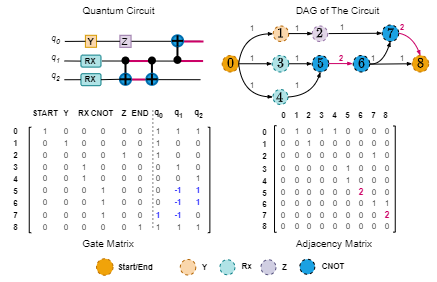
\includegraphics[width = \linewidth]{images/encoding3.drawio.png} %
    \caption{Architecture encoding scheme}
    \label{algorithm-1}
    \end{subfigure}
    \hfill
    \begin{subfigure}{0.5\linewidth}
    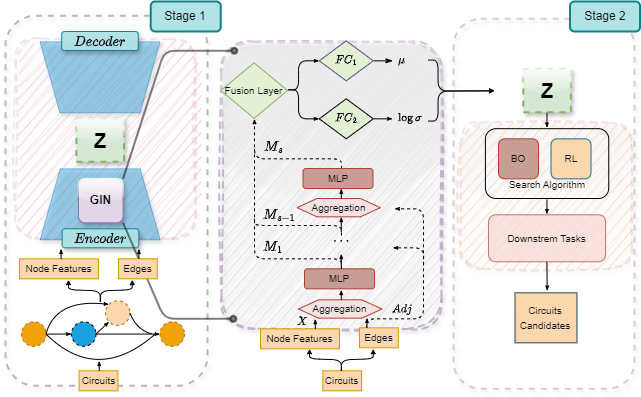
\includegraphics[width = \linewidth]{images/algo_test_2.drawio.png} %
    \caption{Representation learning and search process}
    \label{algorithm-2}
    \end{subfigure}

    \caption{Illustration of our algorithm. In Figure \ref{algorithm-1}, each circuit's architecture is first transformed into a DAG and represented by two matrices. Each row of the gate matrix corresponds to a node in the graph, with one-hot encoding used to indicate the node type, and additional columns encoding position information, such as the qubits the gate acts on. For two-qubit gates, $-1$ and $1$ represent the control and target qubits, respectively. The weights in the adjacency matrix reflect the number of qubits involved in each interaction. In Figure \ref{algorithm-2}, the left side depicts the process of representation learning, where $Z$ represents the latent space of circuit architectures. In the middle, the encoder is shown as the mechanism used to learn this latent space. On the right, Bayesian optimization (BO) and reinforcement learning (RL) are employed to explore the latent space for various quantum machine learning tasks. The algorithm ultimately outputs a set of candidate circuits.}
    \label{algorithm} 
\end{center}
\end{figure}
In this work, we present our method, as illustrated in Figure \ref{algorithm}, which consists of two independent learning components: an autoencoder for circuit architecture representation learning, and a search process that includes both search and evaluation strategies. The search space is defined by the number of gates in a circuit and an operation pool comprising general gate types such as ${\texttt{X, Y, Z, H, Rx, Ry, Rz, U3, CNOT, CY, CZ}}$. A random generator creates a set of circuit architectures based on predefined parameters, including the number of qubits, the number of gates, and the maximum circuit depth. These architectures are then encoded into two matrices and input into the autoencoder. The autoencoder independently learns a latent distribution from the search space and produces pre-trained architecture embeddings for the search algorithms. The evaluation strategy takes the circuit architectures generated by the search algorithm and returns a performance assessment. For evaluating circuit architectures, we use the ground state of a Hamiltonian for max-cut and quantum chemistry problems, and fidelity for quantum state preparation tasks.
%TODO: more introduction for fig 1, 1. search space(random circuits generator,) 2. operation pool, 3 estimation strategy
\subsection{Circuit Encoding Scheme}
We represent quantum circuits as DAGs using the circuit encoding scheme $\mathcal{E}^{GSQAS}$, as described in \citet{he2023gnn, he2023gsqas}. Each circuit is transformed into a DAG by mapping the gates on each qubit to a sequence of nodes, with two additional nodes added to indicate the input and output of circuits. The resulting DAG is described by an adjacency matrix, as shown in Figure \ref{algorithm-1}. The set of nodes is further characterized by a gate matrix, which shows the node features including position information. 

However, the encoding scheme $\mathcal{E}^{GSQAS}$ represents all occupied qubits as $1$ without distinguishing between the control and target positions of two-qubit gates, which limits the effectiveness of circuit representation learning and leads to confusion during circuit reconstruction. Additionally, the adjacency matrix weights do not accurately reflect the original gate connections. To address these limitations, we propose a new encoding scheme. In our method, we explicitly encode positional information for two-qubit gates, such as \texttt{CNOT} and \texttt{CZ}, by assigning $-1$ to the control qubit and $1$ to the target qubit. Furthermore, we represent the number of qubits involved in an edge as the connection weights in the adjacency matrix, as shown in Figure \ref{algorithm-1}. These modifications enhance circuit representation learning and improve the overall effectiveness of the search.
% \begin{figure}[ht]
% \begin{center}
%     \begin{subfigure}[b]{0.325\textwidth}
%     \centering
%     \includegraphics[width=\textwidth]{images/c2g.png} %
%     \caption{Circuit to Graph}
%     \label{c2g}
%     \end{subfigure}
%     \hspace{0.5cm}
%     \begin{subfigure}[b]{0.575\textwidth}
%     \centering
%     \includegraphics[width=\textwidth]{images/encoding-scheme-details.png} %
%     \caption{Gate matrix and adjacency matrix}
%     \label{matrices}
%     \end{subfigure}
%     \caption{Circuit encoding scheme}
%     \label{encodings} 
% \end{center}
% \end{figure}

\subsection{Variational Graph Isomorphism Autoencoder}
\subsubsection{Preliminaries}
The most common graph autoencoders (GAEs) consist of an encoder and a decoder, where the encoder maps a graph into a feature space, and the decoder reconstructs the graph from those features. One prominent example is the variational graph autoencoder (VGAE), a promising framework for unsupervised graph representation learning that utilizes a graph convolutional network as its encoder and a simple inner product as its decoder~\citep{kipf2016variational}. In this work, however, we do not employ the common VGAE as a framework for learning latent representations. Instead, we utilize a more powerful encoder GIN~\citep{xu2019powerful}.

\begin{definition} We are given a circuit created by $m$ gate types, $h$ gates and $g$ qubits. Then, the circuit can be described by a DAG $G=\{V, E\}$ with $n=h+2=|V|$ gate nodes including START and END. The adjacency matrix of graph $G$ is summarized in $n\times n$ matrix $A$ and its gate matrix $X$ is in size of $n \times (m+2+g)$. We further introduce $d$-dimensional latent variables $z_i$ composing latent matrix $Z=\{z_1,..,z_K\}^T$.
\end{definition}

\subsubsection{Encoder}
The encoder GIN maps the structure and node features to latent representations $Z$. An approximation of the posterior distribution $q(Z|X,A)$ is:
\begin{align}
    q(Z|X,A)=\prod^K_{i=1}q(z_i|X,A)\text{,}
\end{align}
where $q(z_i|X,A)=\mathcal{N}(z_i|\mu_i, \text{diag}(\sigma^2_i))$\text{.}
% The mean $\mu_i$ and standard deviation $\sigma_i$ compose the mean and standard deviation matrix:
% \begin{align}
%     \mu=\text{GIN}_\mu(X,\hat{A}),\log\sigma=\text{GIN}_\sigma(X,\hat{A}),
% \end{align}
% where $\hat{A}=A+A^T$.
The $L$-layer GIN generates the embedding matrix $M^{(s)}$ for $s$-layer by:
\begin{align}
    M^{(s)}=MLP^{(s)}((1+\epsilon^{(s)})\cdot M^{(s-1)}+\hat{A}M^{(s-1)}), s=1,2,...,L\text{,}
    \label{mlp}
\end{align}
Where $M^{(0)} = X$, and $\epsilon^{(s)}$ is a bias with a standard normal distribution for each layer. The $MLP$ is a multi-layer perceptron consisting of Linear-BatchNorm-LeakyReLU layers, and $\hat{A} = A + A^T$ transforms a directed graph into an undirected one to capture bi-directional information. In this work, we introduce a new fusion layer, a fully connected layer that aggregates feature information from all GIN layers, rather than just the last one. The mean $\mu = \text{GIN}_\mu(X, \hat{A}) = FC_1(M^{(L)})$ is computed using the fully connected layer $FC_1$, and similarly, the standard deviation $\sigma$ is computed via $FC_2$. We can then sample the latent matrix $Z \sim q(Z|X, A)$ by $z_i = \mu_i + \sigma_i \cdot \epsilon_i$.
For all experiments, we use $L = 5$ GIN layers, a 16-dimensional latent vector $z_i$, and a GIN encoder with hidden sizes of 128. More details on the hyperparameters can be found in Appendix \ref{pretraining_parameters}.
%16-dimensionalcode model line 75, where is the learnable bias $\epsilon$.

\subsubsection{Decoder}
The decoder takes the sampled latent variables $Z$ as input to reconstruct both the adjacency matrix $A$ and the gate matrix $X = [X^t, X^q]$, where $X^t$ encodes the gate types and $X^q$ encodes the qubits on which the gates act. The generative process is summarized as follows:
\begin{align}
     p(A|Z)&=\prod^{K}_{i=1}\prod^{K}_{j=1}p(A_{ij}|z_i,z_j), \text{ with } p(A_{ij}|z_i,z_j)=\text{ReLU}_j(F_{1}(z^T_iz_j))\text{,}\\
     p(X|Z)&=\prod^K_{i=1}p(x_i|z_i)\text{,}
     \text{ with } p(x^t_i|z_i)=\text{softmax}(F_{2}(z_i))\text{, } p(x^q_i|z_i)=\text{tanh}(F_{2}(z_i))\text{,}
\end{align}
where both $F_{1}$ and $F_{2}$ are trainable linear functions.

%\begin{align}
%p(A|Z)&=\prod^{K}_{i=1}\prod^{K}_{j=1}p(A_{ij}|z_i,z_j), \text{ %with } p(A_{ij}=1|z_i,z_j)=\text{ReLU}_j(F_{\text{adj}}%(z^T_iz_j))\text{,}
%\end{align}
%where $F_{\text{adj}}$ is trainable linear function. A similar process applies for $X$.

\subsubsection{Objective Function}
The weights in the encoder and decoder are optimized by maximizing the evidence lower bound (ELBO) $\mathcal{L}$, which is defined as:
\begin{align}
    \mathcal{L}=E_{q(Z|X,A)}[\log p(X^{\text{type}},X^{\text{qubit}},A|Z)]-\text{KL}[(q(Z|X,A))||p(Z)]\text{,}
\end{align}
where KL$[q(\cdot)||p(\cdot)]$ represents the Kullback-Leibler (KL) divergence between $q(\cdot)$ and $p(\cdot)$. We further adopt a Gaussian prior $p(Z)=\prod_i \mathcal{N}(z_i|0,I)$. The weights are optimized using minibatch gradient descent, with a batch size of 32.
\subsection{Architecture Search Strategies}
\subsubsection{Reinforcement Learning (RL)}
%TODO check with zixin REINFORCE, latent vector, check layer LSTM
After conducting initial trials with PPO~\citep{schulman2017proximal} and A2C~\citep{huang2022a2c}, we adopt REINFORCE~\citep{Williams:92} as a more effective reinforcement learning algorithm for architecture search. In this approach, the environment's state space consists of pre-trained embeddings, and the agent uses a one-cell LSTM as its policy network. The agent selects an action, corresponding to a sampled latent vector based on the distribution of the current state, and transitions to the next state based on the chosen action. The reward for max-cut and quantum chemistry tasks is defined as the ratio of energy to ground energy, with values outside the range [0, 1] clipped to 0 or 1. For the state preparation task, circuit fidelity is used as the reward.
We employ an adaptive batch size, with the number of steps per training epoch determined by the average reward of the previous epoch. Additionally, we use a linear adaptive baseline, defined by the formula $B = \alpha \cdot B + (1 - \alpha) \cdot R_{avg}$, where $B$ denotes the baseline, $\alpha$ is a predefined value in the range [0,1], and $R_{avg}$ is the average reward. Each run in this work involves 1000 searches.

\subsubsection{Bayesian Optimization (BO)}
As another search strategy used in this work without labeling, we employ Deep Networks for Global Optimization (DNGO)\citep{snoek2015scalable} in the context of BO. We adopt a one-layer adaptive BO regression model with a basis function extracted from a feed-forward neural network, consisting of 128 units in the hidden layer, to model distributions over functions. Expected Improvement (EI)\citep{conf/ifip/Mockus77} is selected as the acquisition function. EI identifies the top-k embeddings for each training epoch, with a default objective value of 0.9. The training begins with an initial set of 16 samples, and in each subsequent epoch, the top-k architectures proposed by EI are added to the batch. The network is retrained for 100 epochs using the architectures from the updated batch. This process is iterated until the predefined number of search iterations is reached.

\section{Experimental Results}
To demonstrate the effectiveness and generalization capability of our approach, we conduct experiments on three well-known quantum computing applications: quantum state preparation, max-cut, and quantum chemistry. For each application, we start with a simple example involving 4 qubits and then progress to a more complex example with 8 qubits. We utilize a random generator to create 100,000 circuits as the search space, and all experiments are performed on a noise-free simulator during the search process. Detailed settings are provided in Appendix \ref{application_setting}. We begin by evaluating the model's pre-training performance for unsupervised representation learning (§\ref{pretraning_performance}), followed by an assessment of QAS performance based on the pre-trained latent representations (§\ref{qas_performance}).

\subsection{Pre-training Performance}
\label{pretraning_performance}
\textbf{Observation (1):} GAE and VGAE \citep{kipf2016variational} are two popular baselines for NAS. In an attempt to find models capable of capturing superior latent representations of quantum circuit architectures, we initially applied these two well-known models. However, due to the increased complexity of quantum circuit architectures compared to neural network architectures, these models failed to deliver the expected results. In contrast, models based on GINs \citep{xu2019powerful} successfully obtained valid latent representations, attributed to their more effective neighbor aggregation scheme.
Table \ref{model_performance} presents a performance comparison between the original model using the $\mathcal{E}^{GSQAS}$ encoding and the improved model with our enhanced encoding for 4, 8, and 12 qubit circuits, evaluated across five metrics: Accuracy${ops}$, which measures the reconstruction accuracy of gate types in the gate matrix for the held-out test set; Accuracy${qubit}$, which reflects the reconstruction accuracy of qubits that the gates act on; Accuracy${adj}$, which measures the reconstruction accuracy of the adjacency matrix; Falpos${mean}$, which represents the mean false positives in the reconstructed adjacency matrix; and KLD (KL divergence), which indicates the continuity and smoothness of the latent representation.
The results in the table indicate that the improved model with our enhanced encoding achieves comparable or better than the original. This improvement can be attributed to two factors: first, the new encoding better captures the specific characteristics of the circuits, and second, the fusion of outputs from multiple layers of GIN helps retain shallow information, resulting in more stable training.
\begin{table} [ht]
    \footnotesize
    \centering
    \begin{tabular}{ l l|l l l l l}
    \hline
    \multirow{2}{*}{Qubit}&
    \multirow{2}{*}{Model}&
    \multicolumn{5}{c}{Metric}\\
    \cline{3-7}
    & & Accuracy$_{ops}$ & Accuracy$_{qubit}$ & Accuracy$_{adj}$ & Falpos$_{mean}$ & KLD\\
    \hline
    4 & GSQAS & 99.99 & 99.99 & 99.91 & 100.00 & 0.061\\
    \hline
    4 & Ours & \textbf{100} & 99.97 & 98.89 & \textbf{23.41} & \textbf{0.045}\\
    \hline
    8 & GSQAS & 86.69 & 99.98 & 99.82 & 100.00 & 0.038\\
    \hline
    8 & Ours & \textbf{100} & 98.65 & 97.34 & \textbf{7.35} & \textbf{0.029}\\
    \hline
    12 & GSQAS & 86.69 & 99.94 & 99.70 & 100.00 & 0.028\\
    \hline
    12 & Ours & \textbf{98.67} & 99.14 & 97.79 & \textbf{4.75} & \textbf{0.022}\\
    \hline
    \end{tabular}
    \caption{Pretraining model performance of 4-, 8-, and 12-qubit circuits across the four metrics.}
    \label{model_performance}
\end{table}

\textbf{Observation (2):} In Figure \ref{2D-Visu}, we employ two popular techniques, PCA \citep{shlens2014tutorial} and t-SNE \citep{van2008visualizing}, to visualize the high-dimensional latent representations of 4- and 12-qubit quantum machine learning (QML) applications based on our pre-trained models. The results highlight the effectiveness of our new encoding approach for unsupervised clustering and high-dimensional data visualization. The figures show that the latent representation space of quantum circuits is smooth and compact, with architectures of similar performance clustering together when the search space is limited to 4 qubits. Notably, high-performance quantum circuit architectures are concentrated on the right side of the visualizations. In particular, PCA yields exceptionally smooth and compact representations with strong clustering effects, making it easier and more efficient to conduct QAS within such a structured latent space. This provides a robust foundation for our QAS algorithms.

For the 12-qubit latent space, high-performance circuits (shown in red) are less prominent, likely due to the fact that the 100,000 circuit structures represent only a finite subset of the possibilities for 12-qubit circuit. As a result, the number of circuits that can be learned is limited. Most high-performance circuits are distributed along the left edge of the latent space, with a color gradient transitioning from dark to light as one moves from right to left.

Compared with subfigures \ref{fig:Prev PCA-4 QC}, \ref{fig:Prev PCA-4 Maxcut}, \ref{fig:Prev PCA-4 Fidelity}, \ref{fig: Prev t-SNE-4 vqe}, \ref{fig:Prev t-SNE 4 maxcut}, and \ref{fig:Prev PCA-4 Fidelity}, which utilize the encoding scheme $\mathcal{E}^{GSQAS}$ and show more loosely distributed red points, our new encoding results in a more concentrated and smoother latent representation, as demonstrated in subfigures \ref{fig:PCA-4}, \ref{fig:PCA-4-Max-cut} and \ref{fig:PCA-4-Fidelity}.

\begin{figure}[ht]
    \centering
    % First row
    
    \begin{subfigure}{0.23\textwidth}
        \centering
        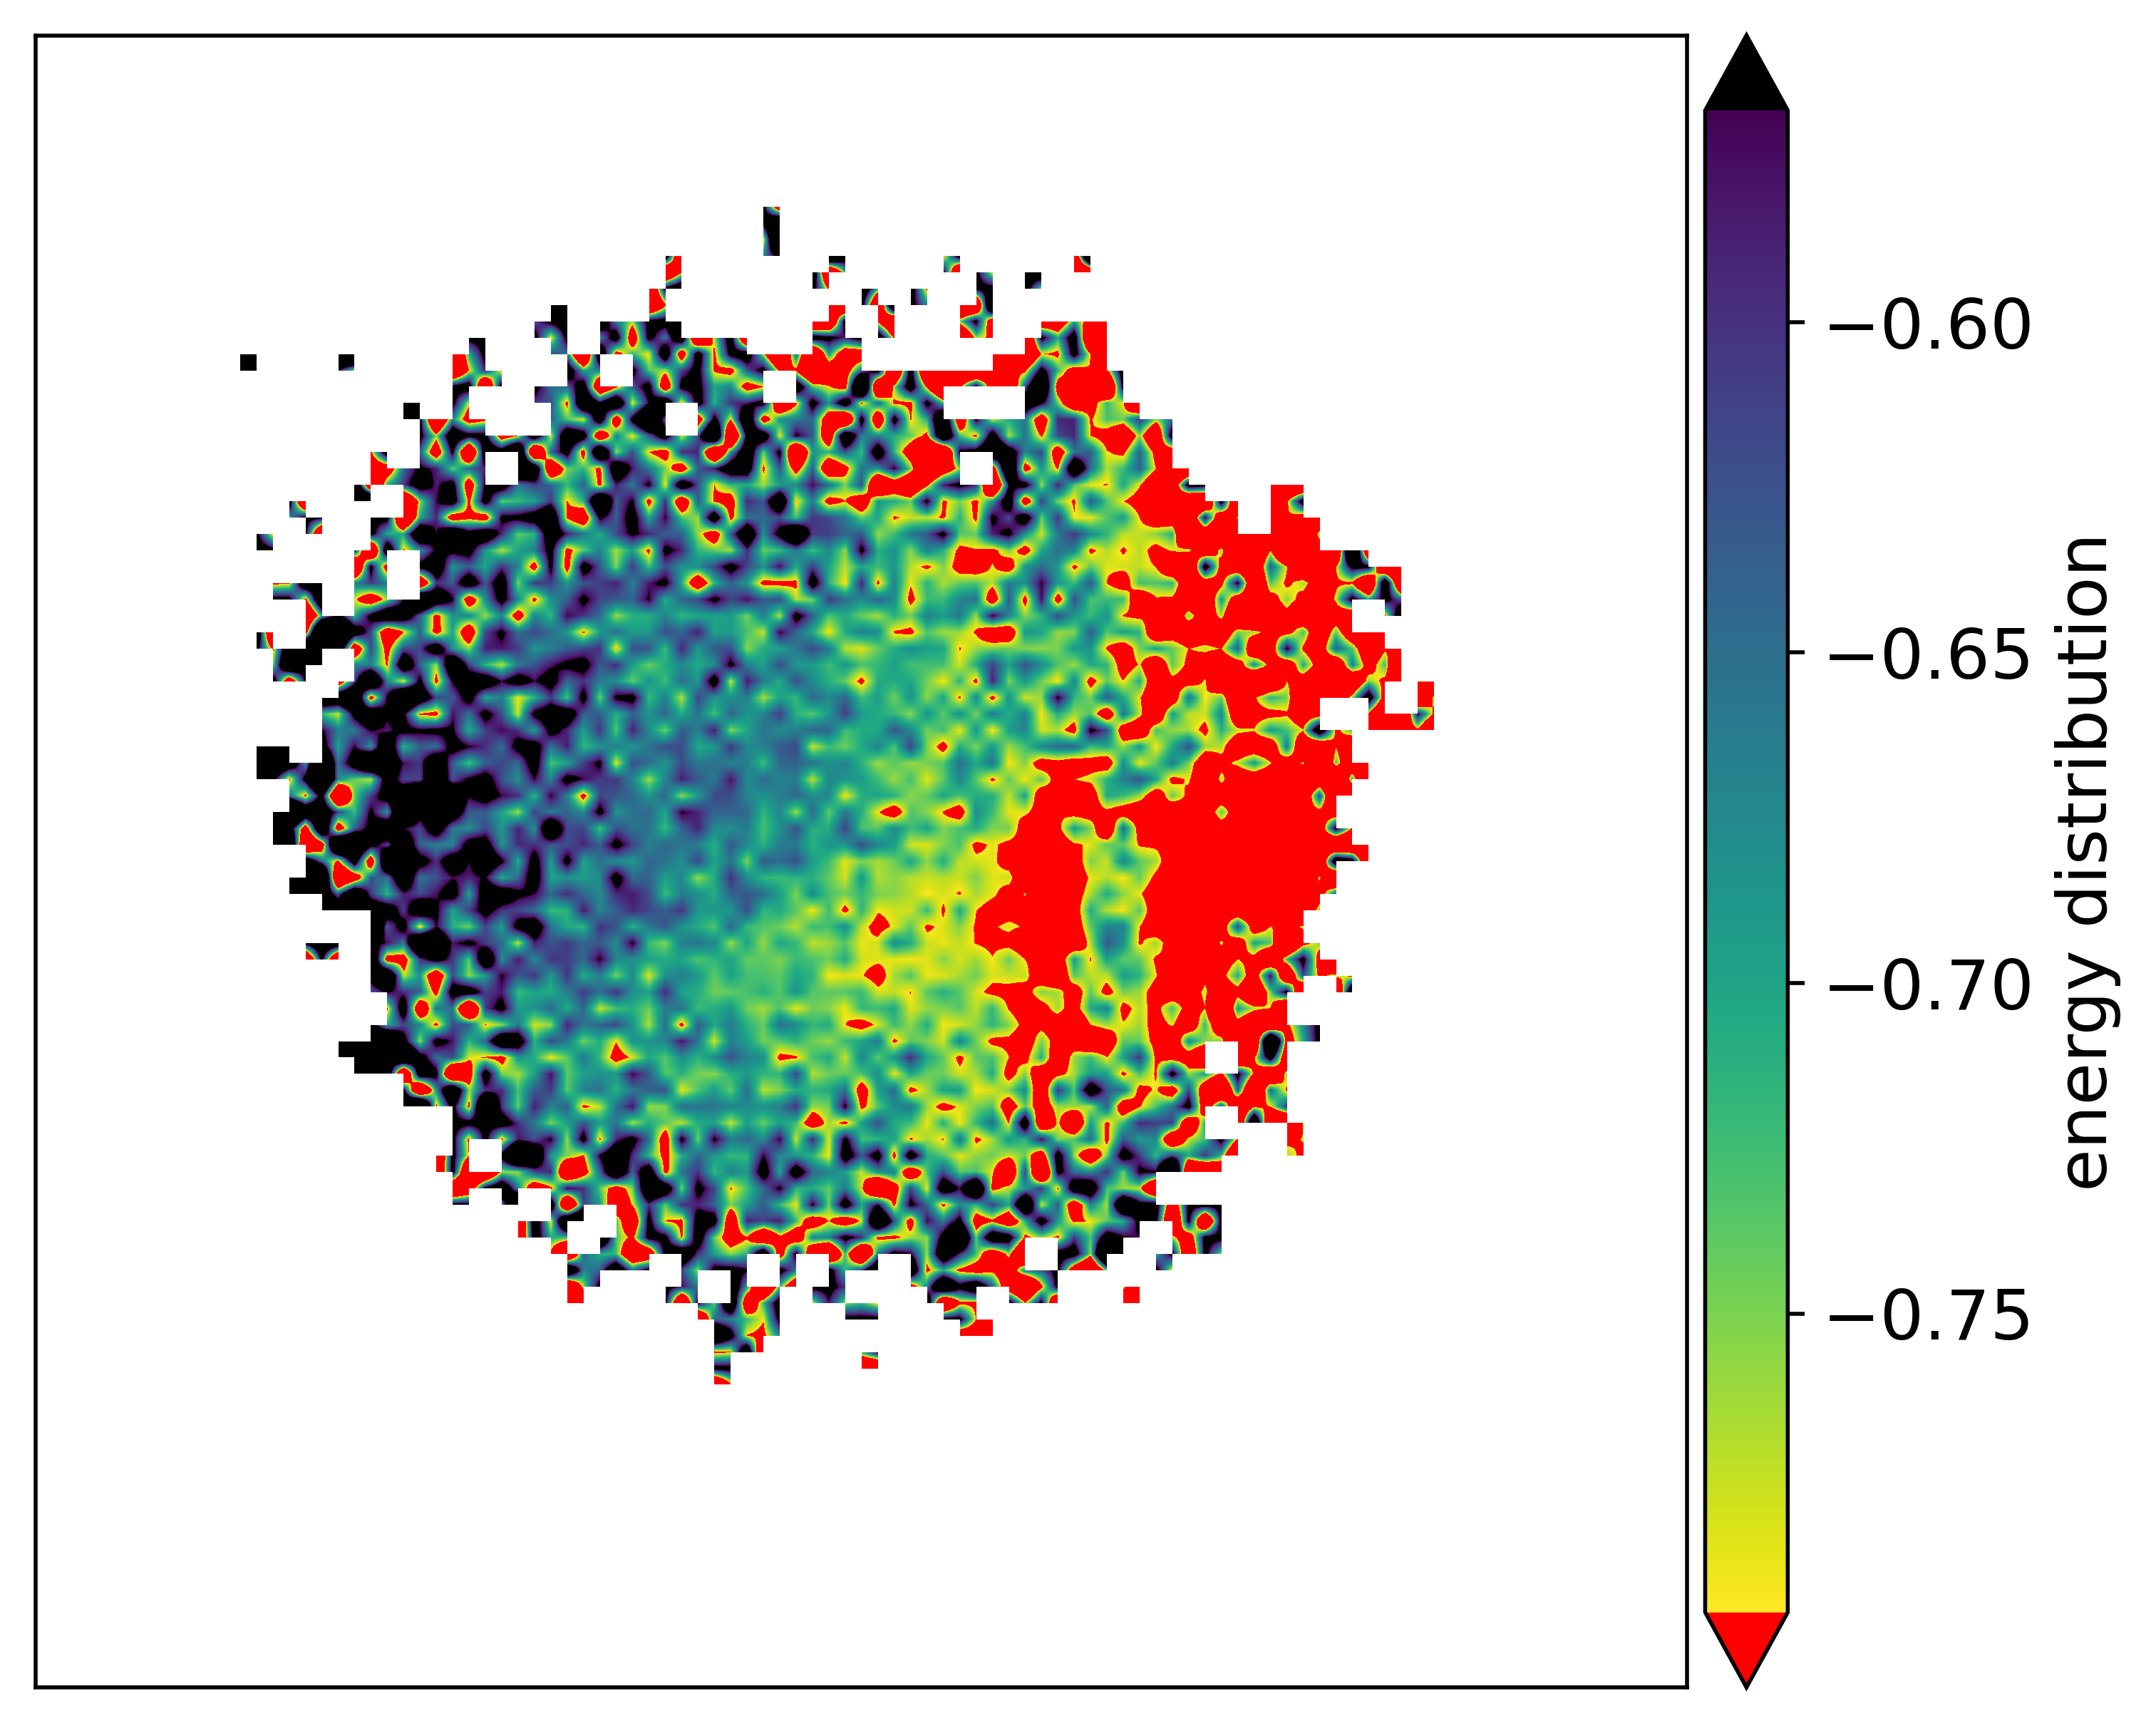
\includegraphics[width=\textwidth]{images/vqe-model-circuits_4_qubits_quantum_arch2vec_full_embedding_full_embedding_smooth.png}
        \caption{PCA$_4$ QC$_{H_2}$}
        \label{fig:PCA-4}
    \end{subfigure}
    %\hspace{0.02\textwidth}
    \begin{subfigure}{0.23\textwidth}
        \centering
        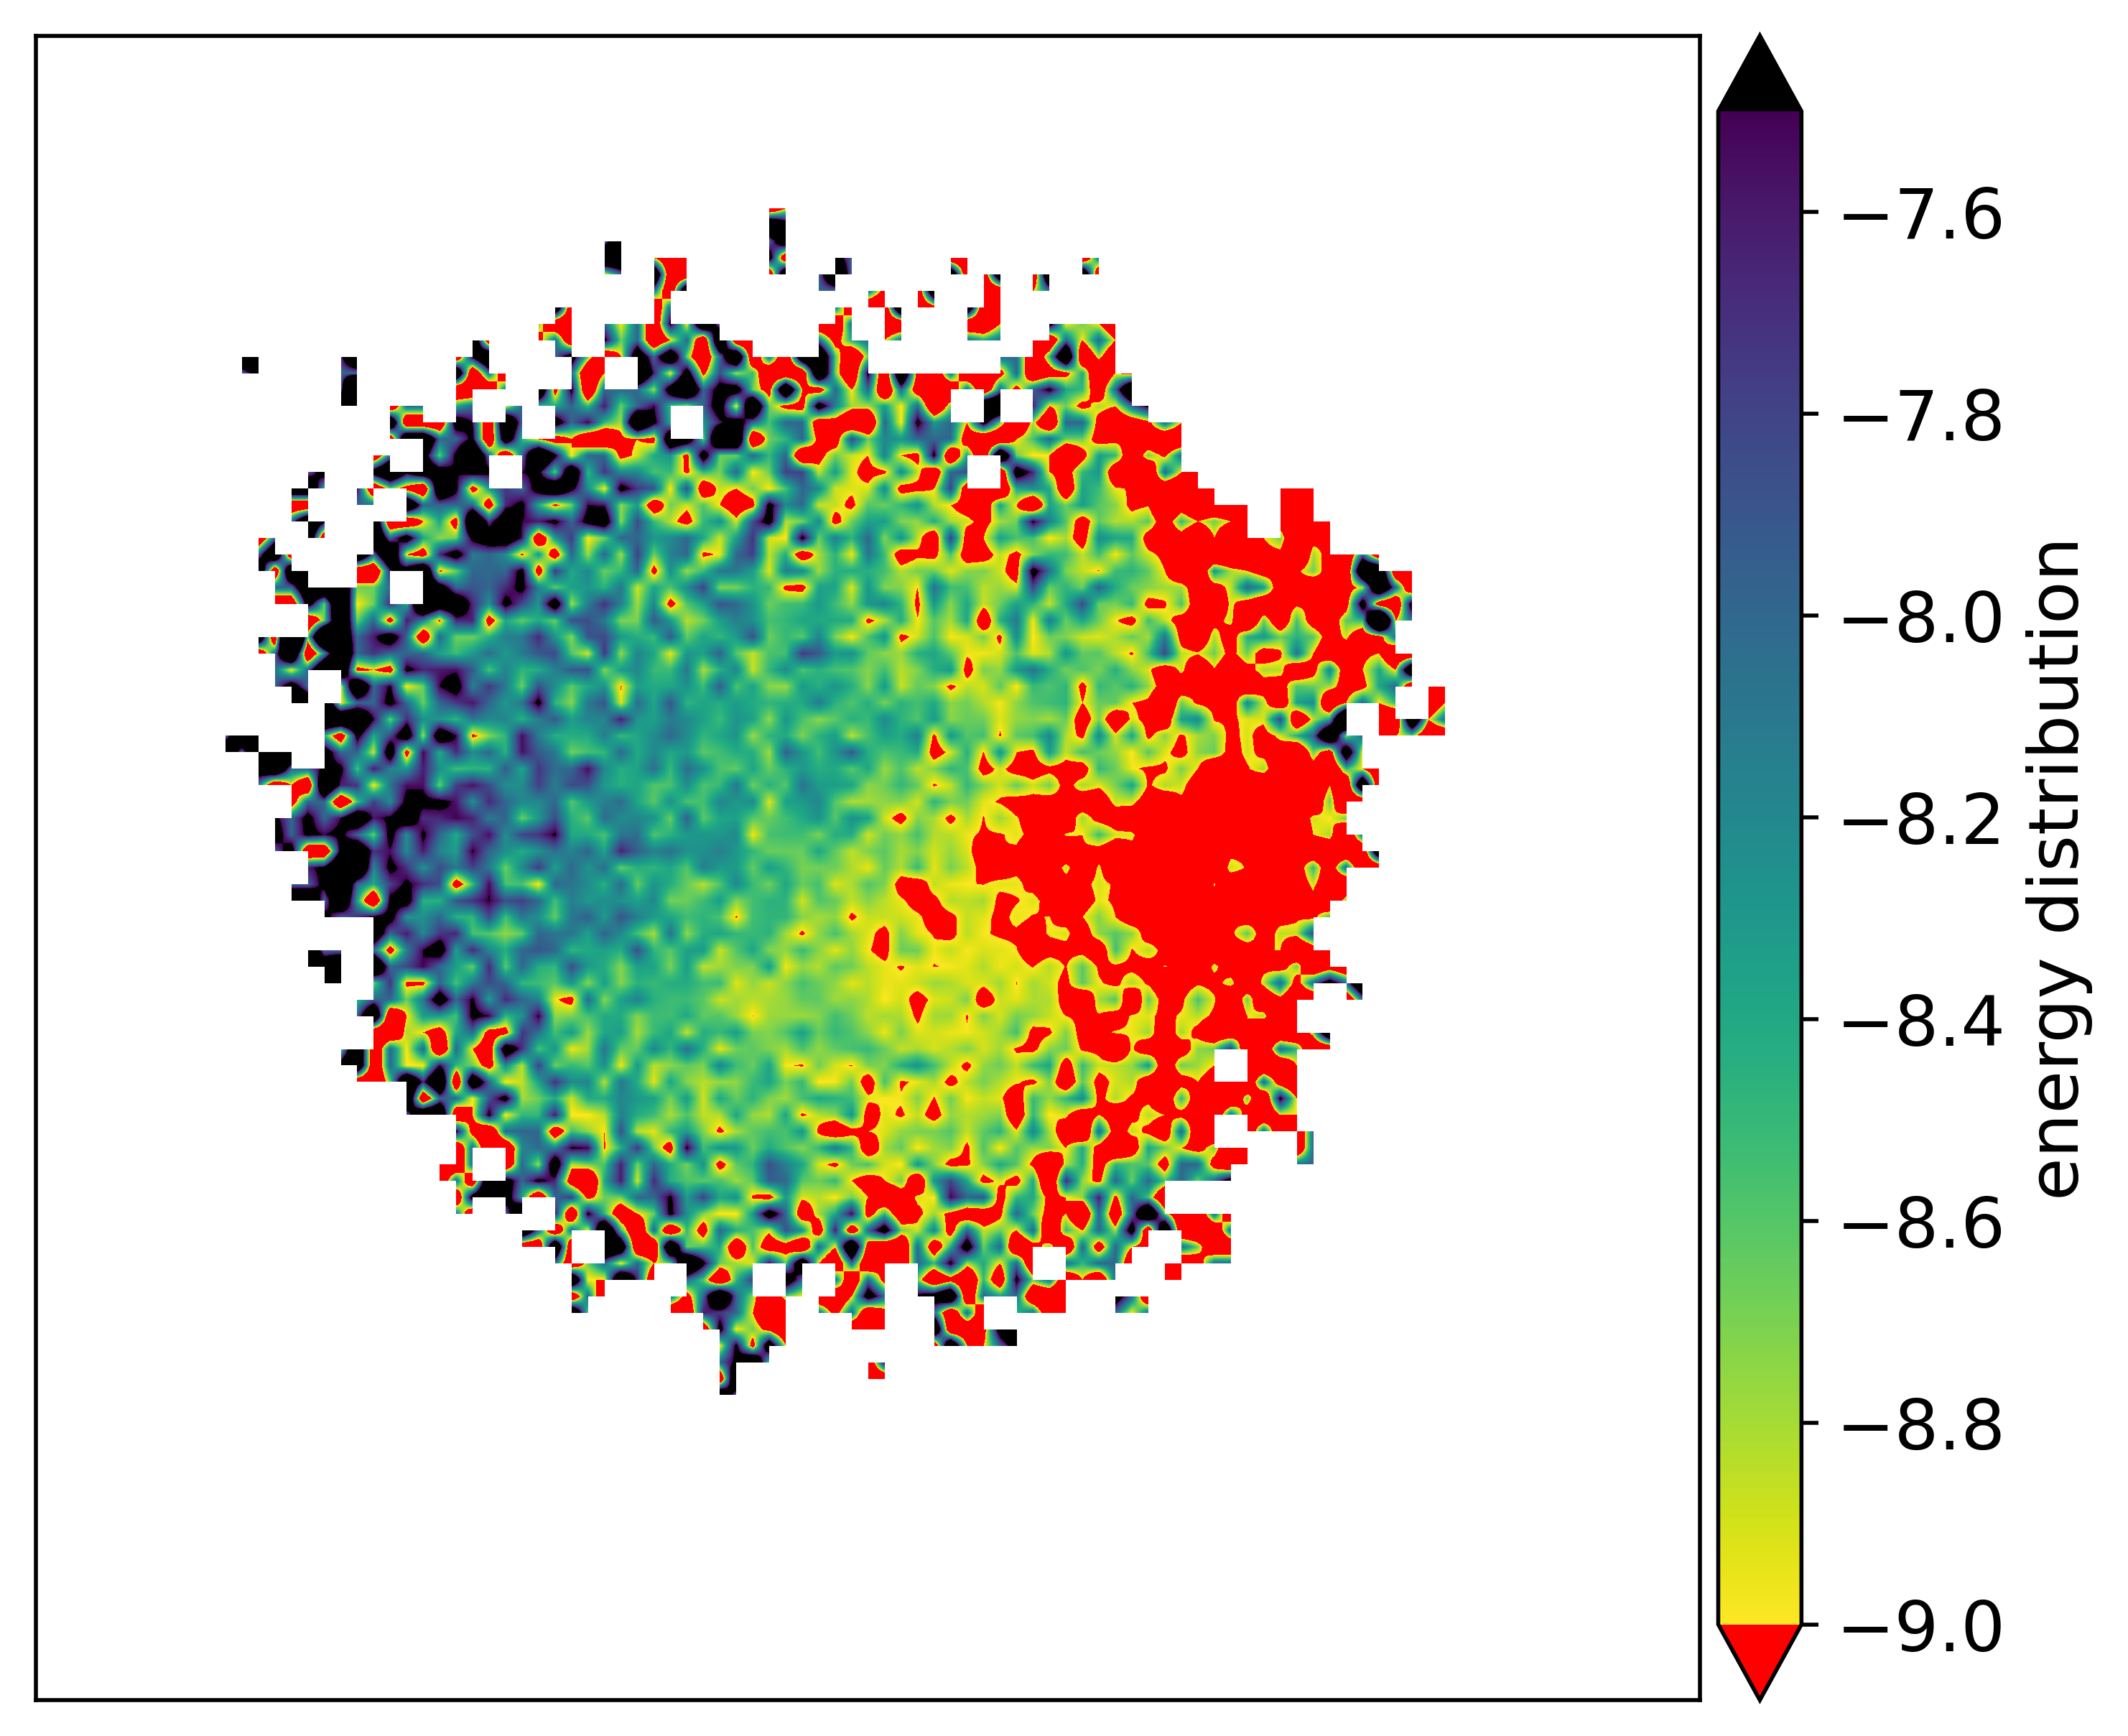
\includegraphics[width=\textwidth]{images/maxcut-model-circuits_4_qubits_quantum_arch2vec_full_embedding_full_embedding_smooth.png}
        \caption{PCA$_4$ Max-cut}
        \label{fig:PCA-4-Max-cut}
    \end{subfigure}
    \begin{subfigure}{0.23\textwidth}
        \centering
        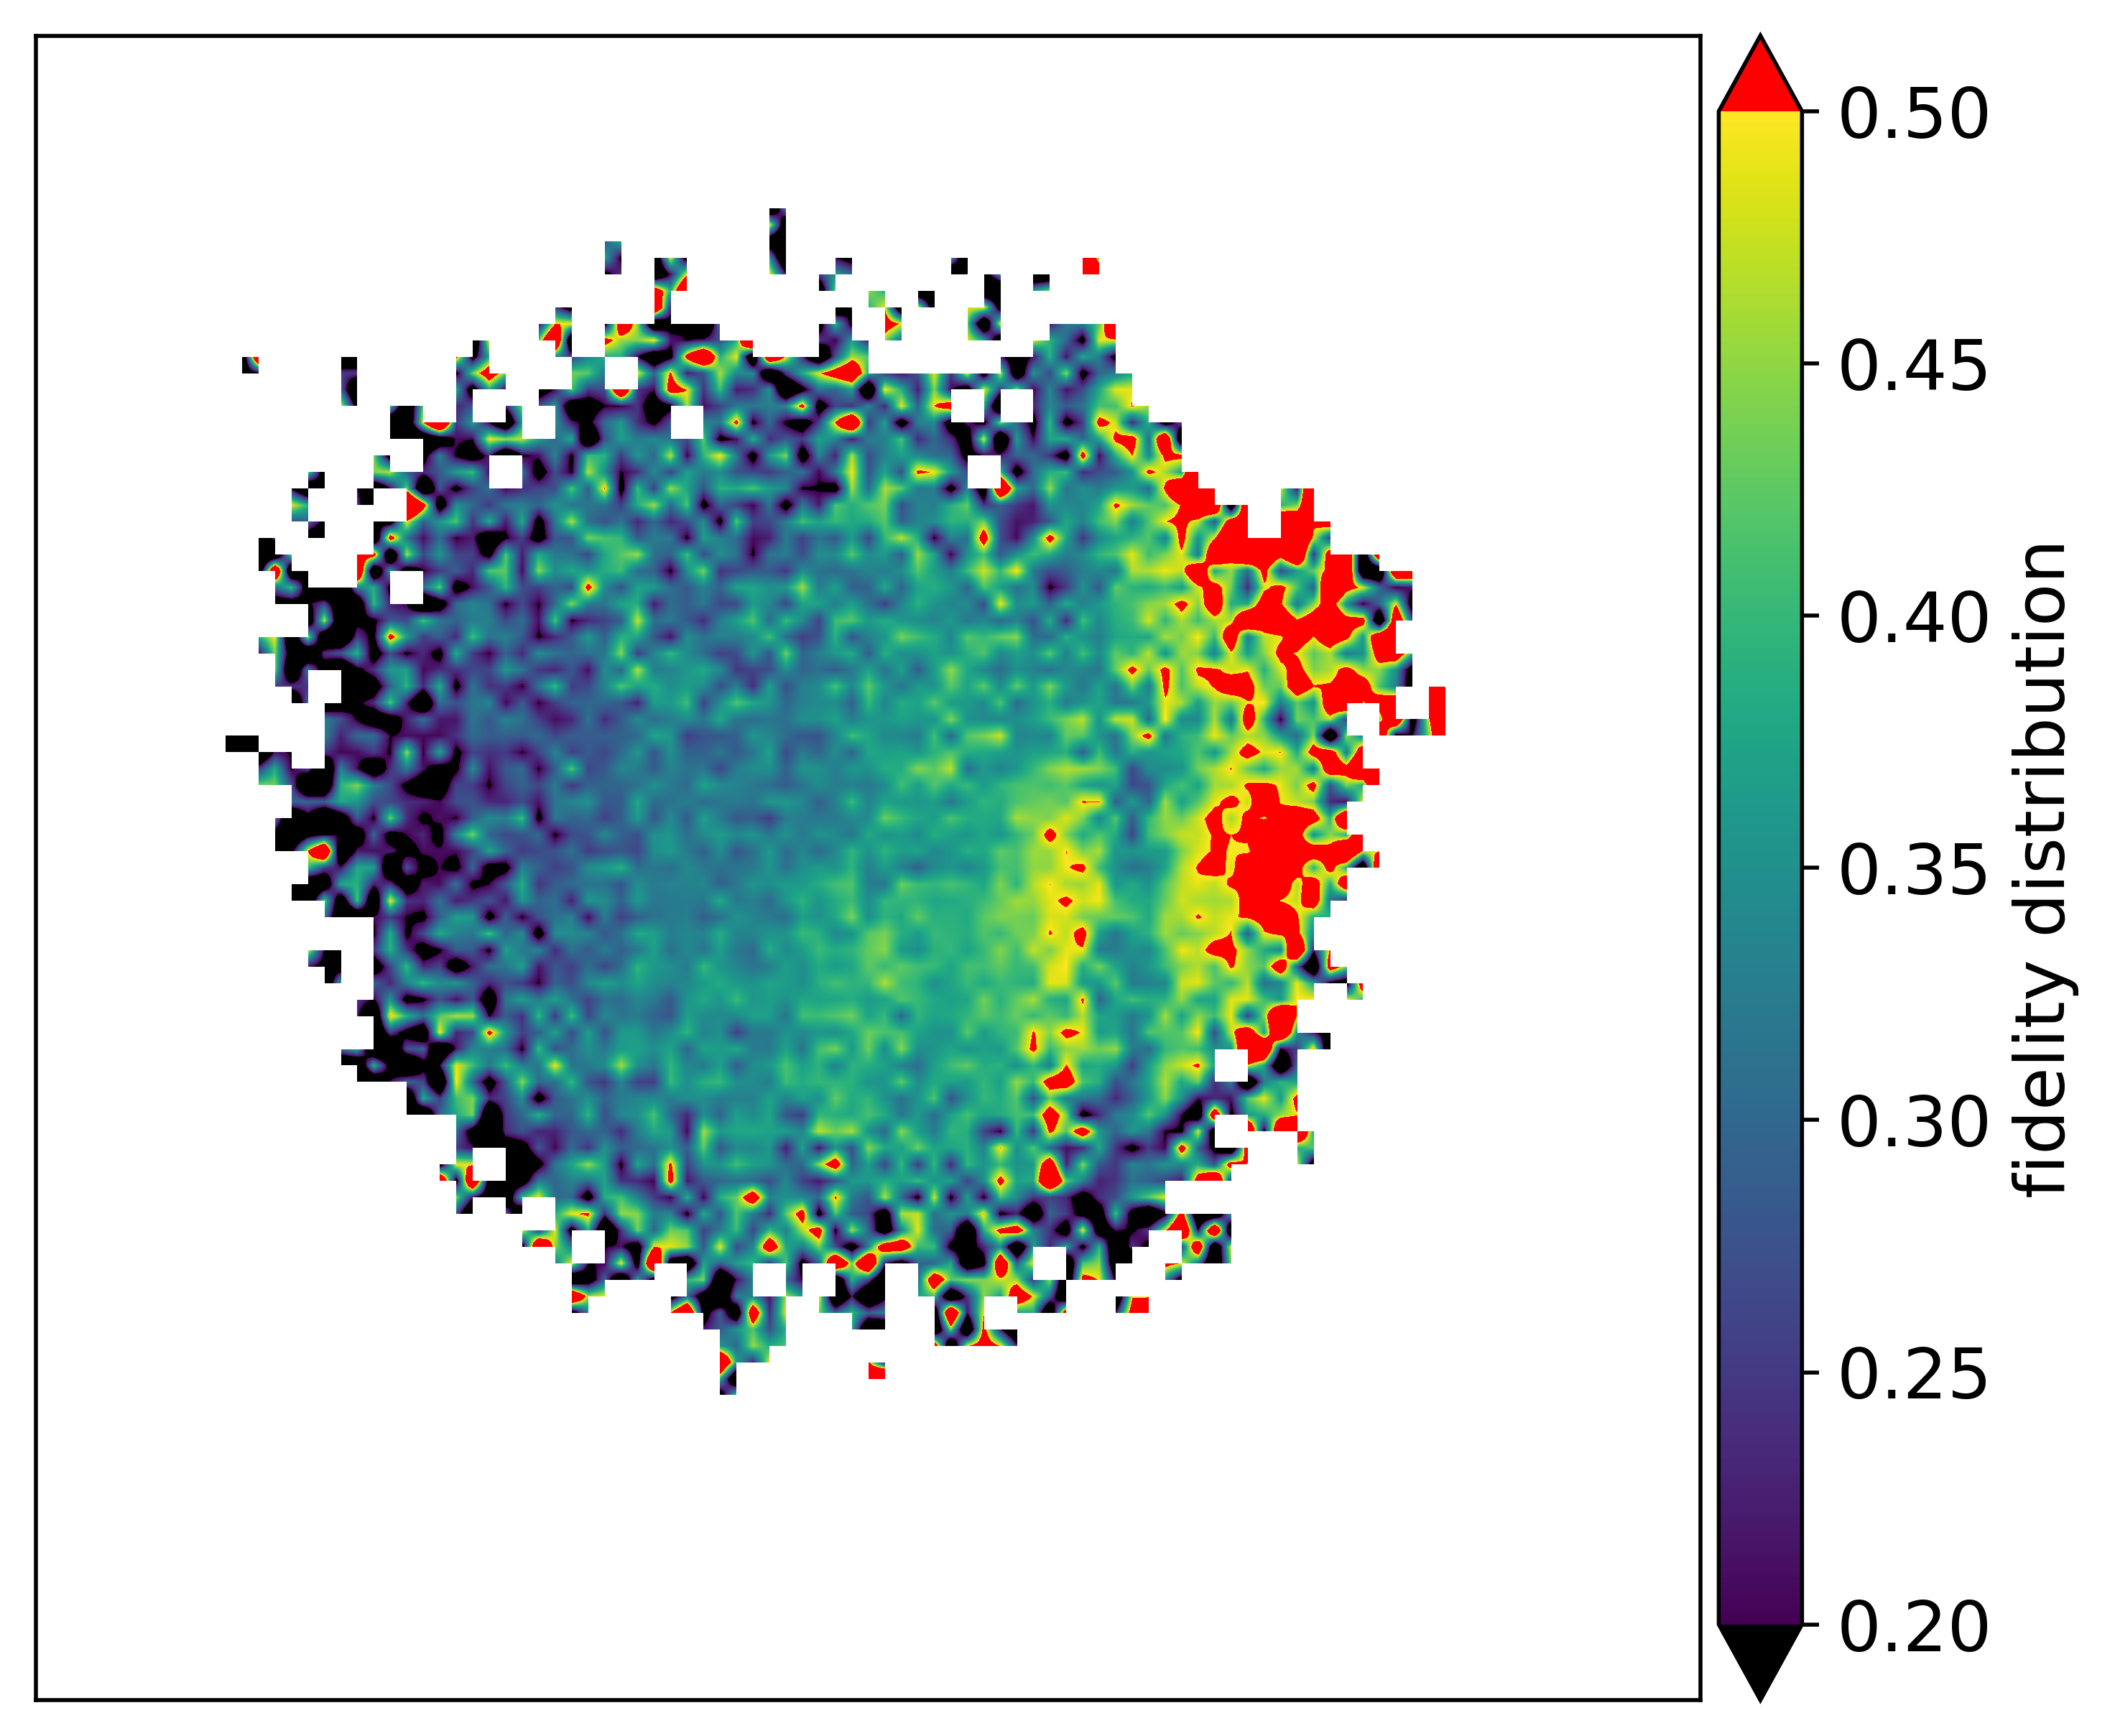
\includegraphics[width=\textwidth]{images/fidelity-model-circuits_4_qubits_quantum_arch2vec_full_embedding_full_embedding_smooth.png}
        \caption{PCA$_4$ Fidelity}
        \label{fig:PCA-4-Fidelity}
    \end{subfigure}
    \begin{subfigure}{0.23\textwidth}
        \centering
        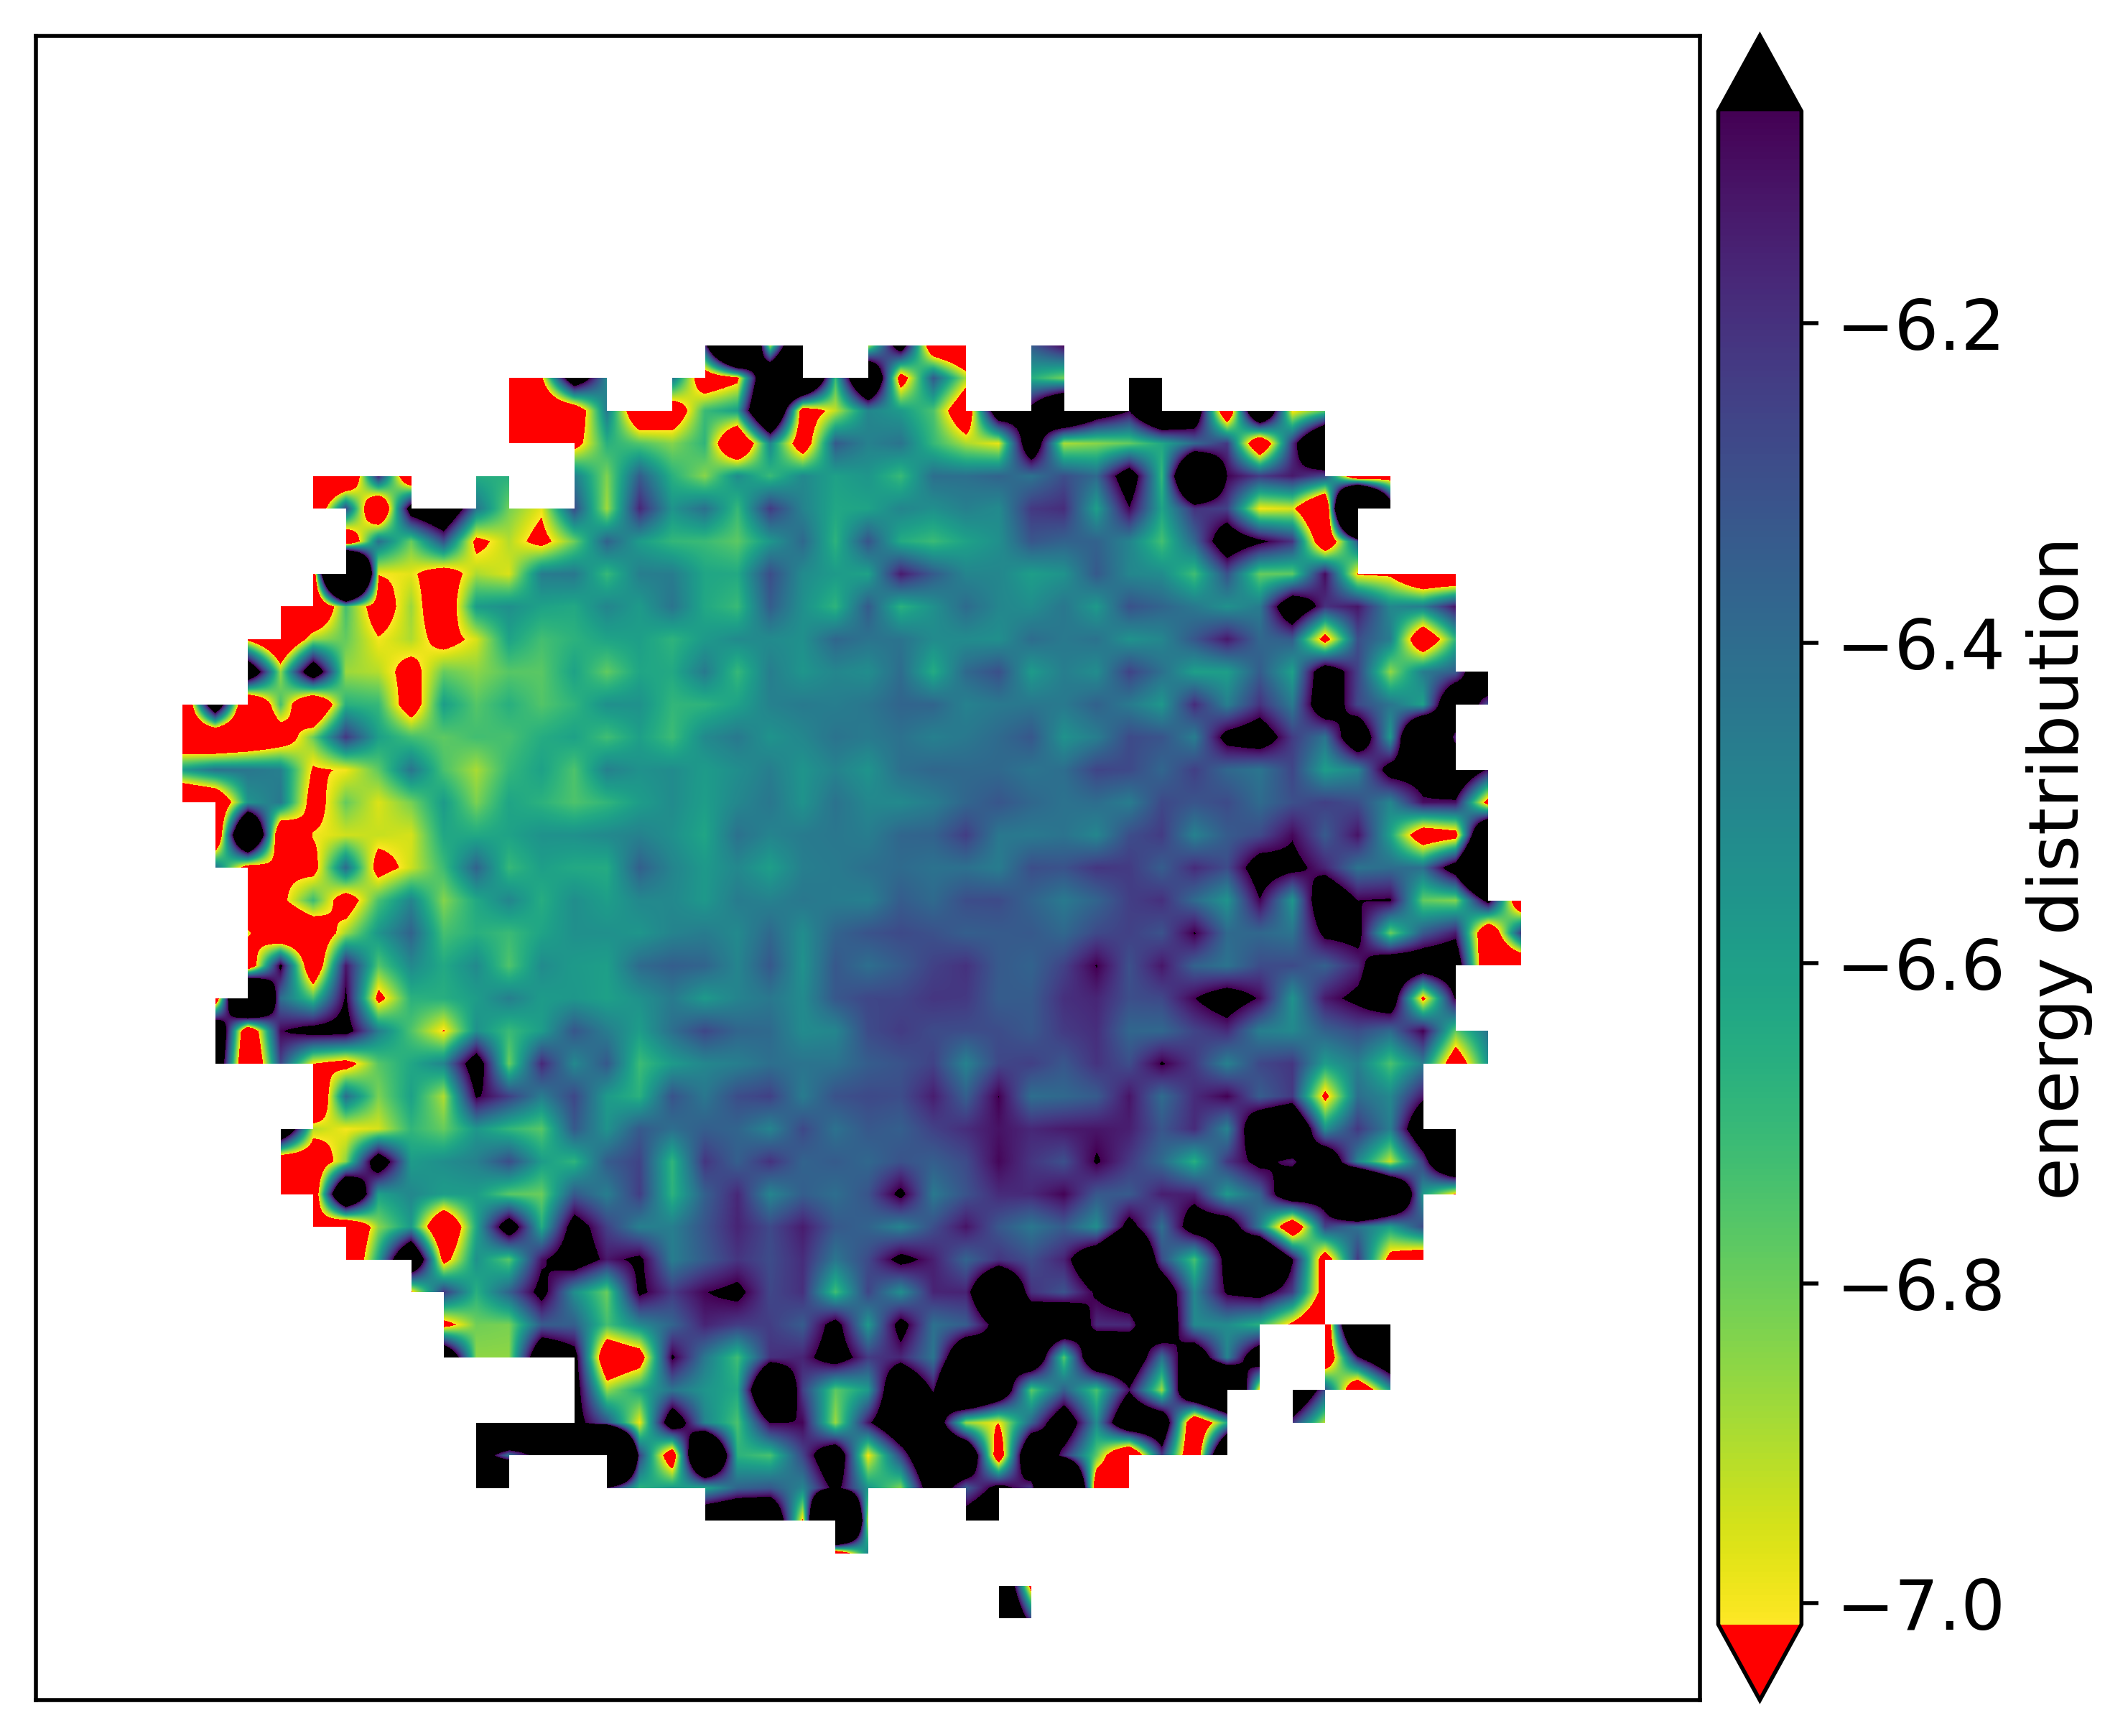
\includegraphics[width=\textwidth]{images/vqe-model-circuits_12_qubits_quantum_arch2vec_full_embedding_full_embedding_smooth.png}
        \caption{PCA$_{12}$ QC$_{LiH}$}
        \label{fig:PCA-12}
    \end{subfigure}
    
    % Second row
    \begin{subfigure}{0.23\textwidth}
        \centering
        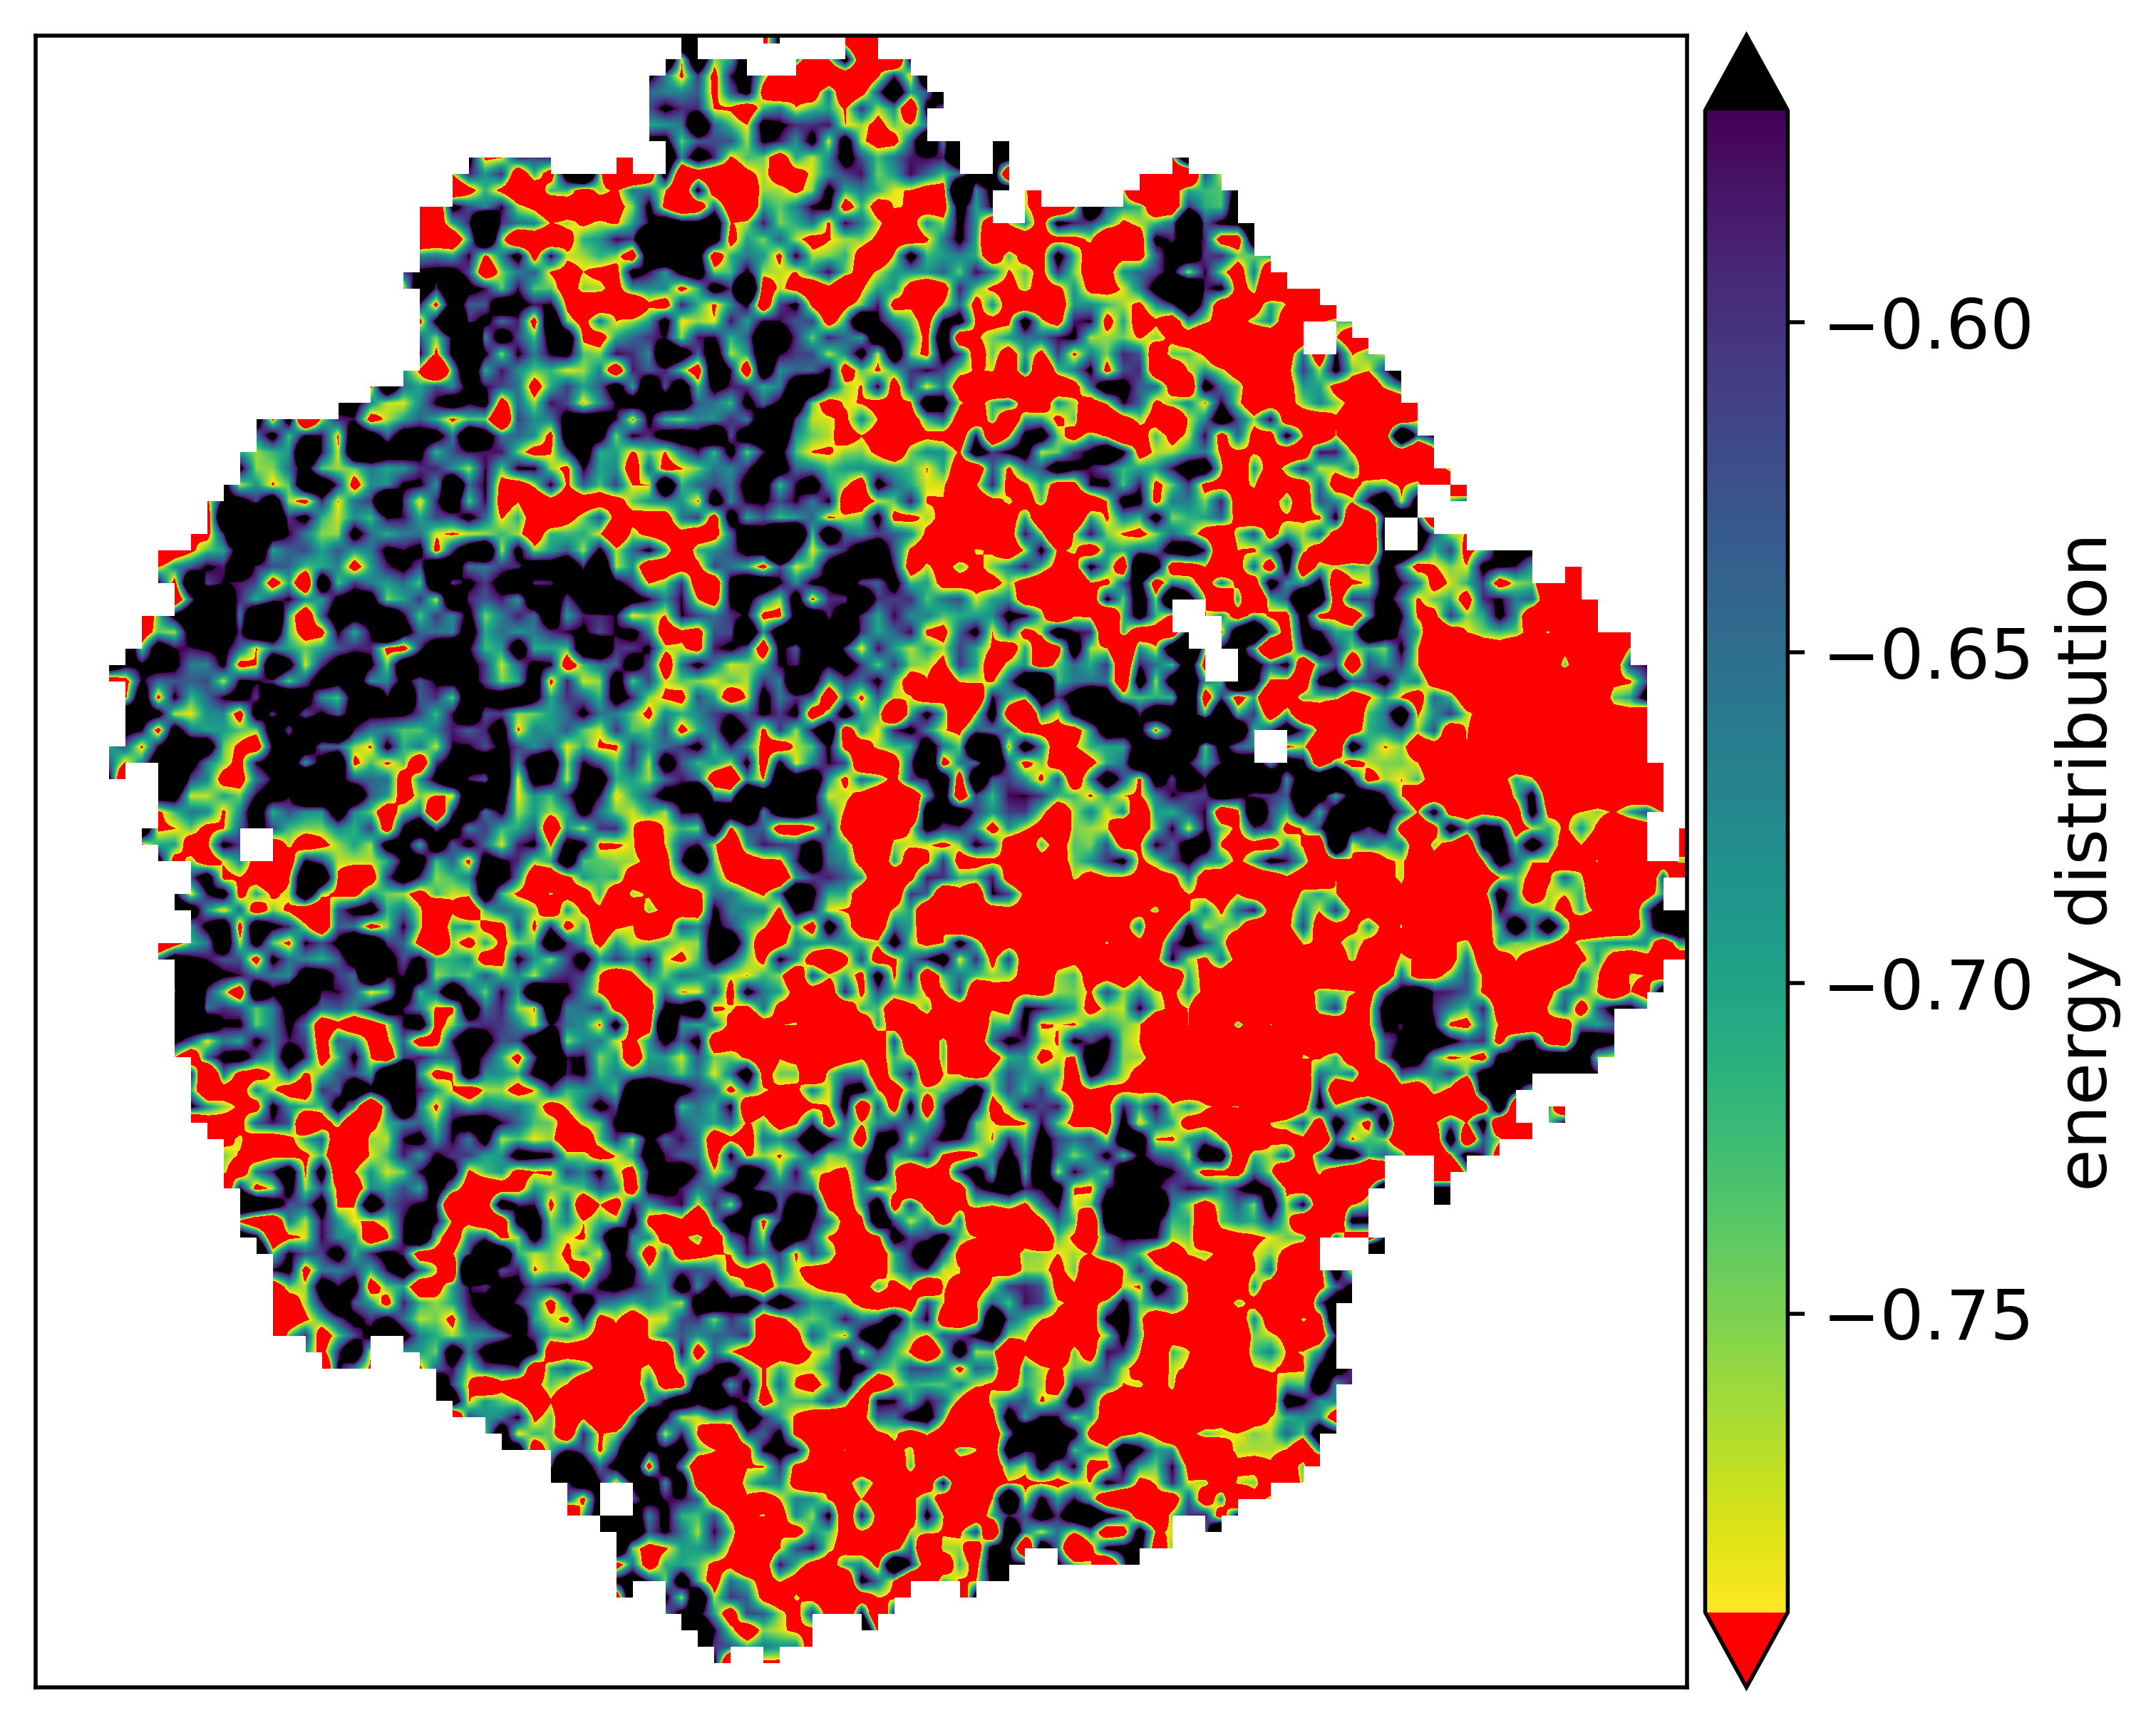
\includegraphics[width=\textwidth]{images/tsqe/vqe-model-circuits_4_qubits_quantum_arch2vec_full_embedding_full_embedding_smooth.png}
        \caption{t-SNE$_4$ QC$_{H_2}$}
        \label{fig:t-SNE-4}
    \end{subfigure}
    %\hspace{0.02\textwidth}
    \begin{subfigure}{0.23\textwidth}
        \centering
        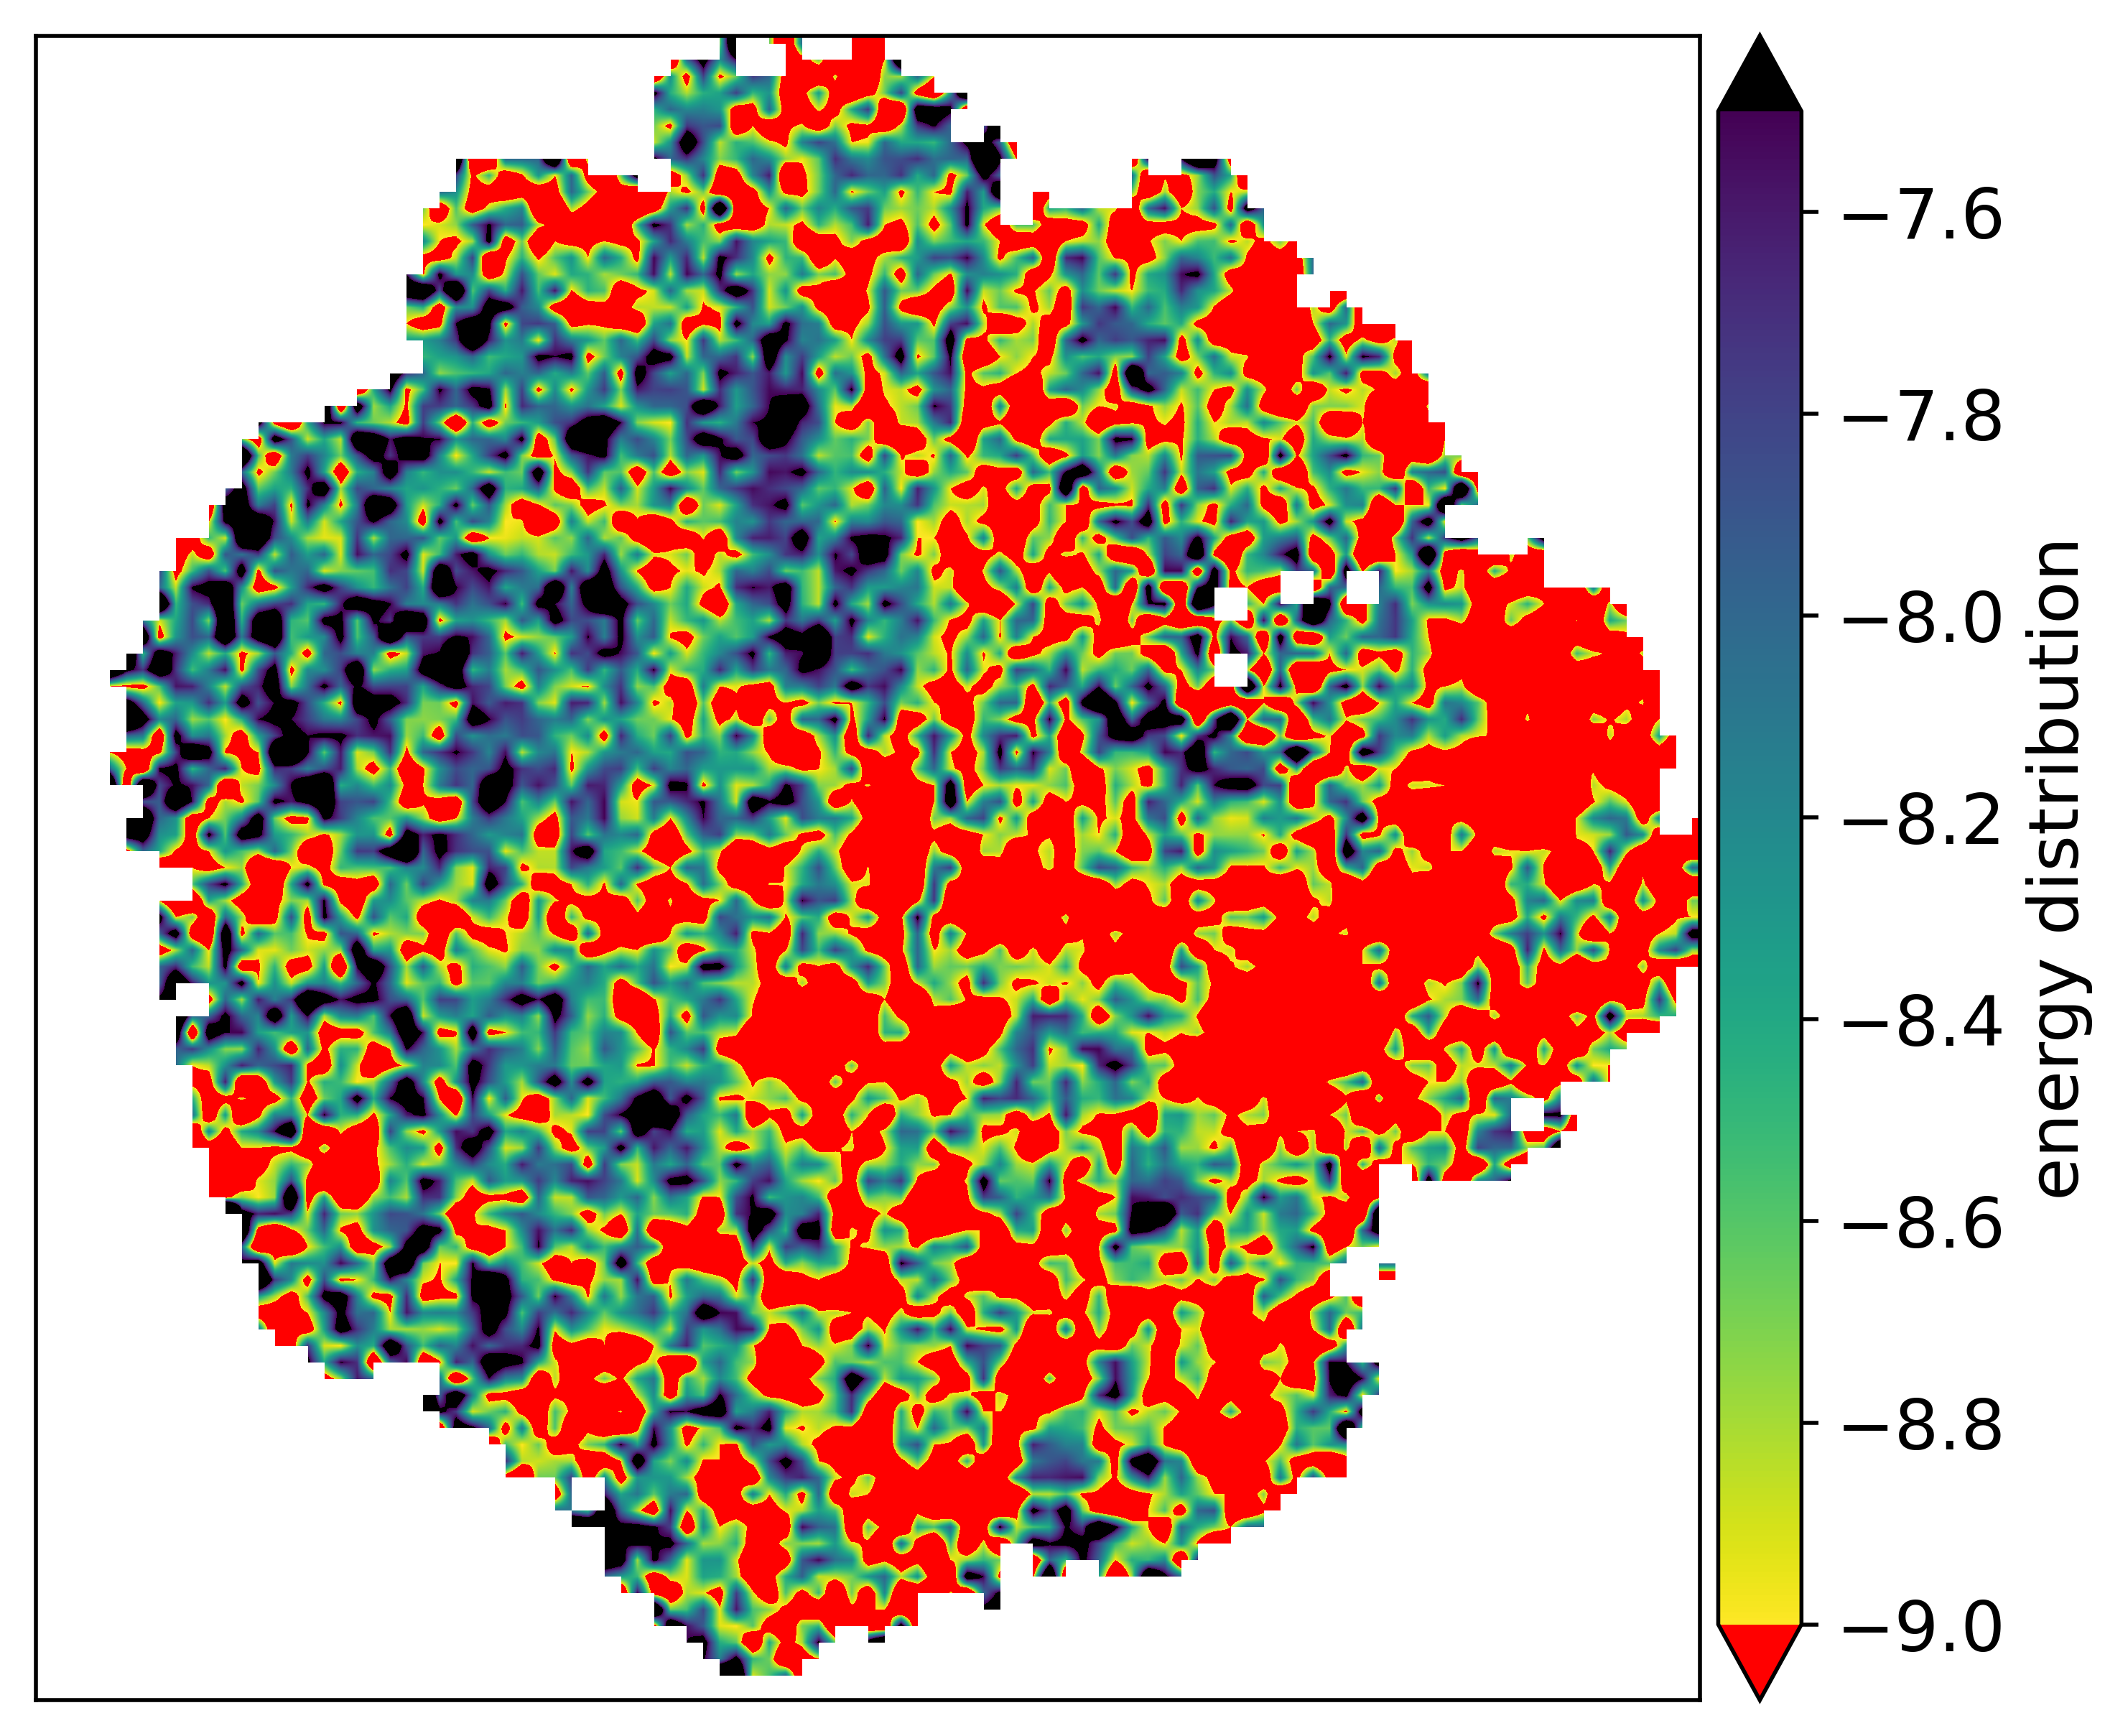
\includegraphics[width=\textwidth]{images/tsqe/maxcut-model-circuits_4_qubits_quantum_arch2vec_full_embedding_full_embedding_smooth.png}
        \caption{t-SNE$_4$ Max-cut}
        \label{fig:t-SNE4 Maxcut}
    \end{subfigure}
    \begin{subfigure}{0.23\textwidth}
        \centering
        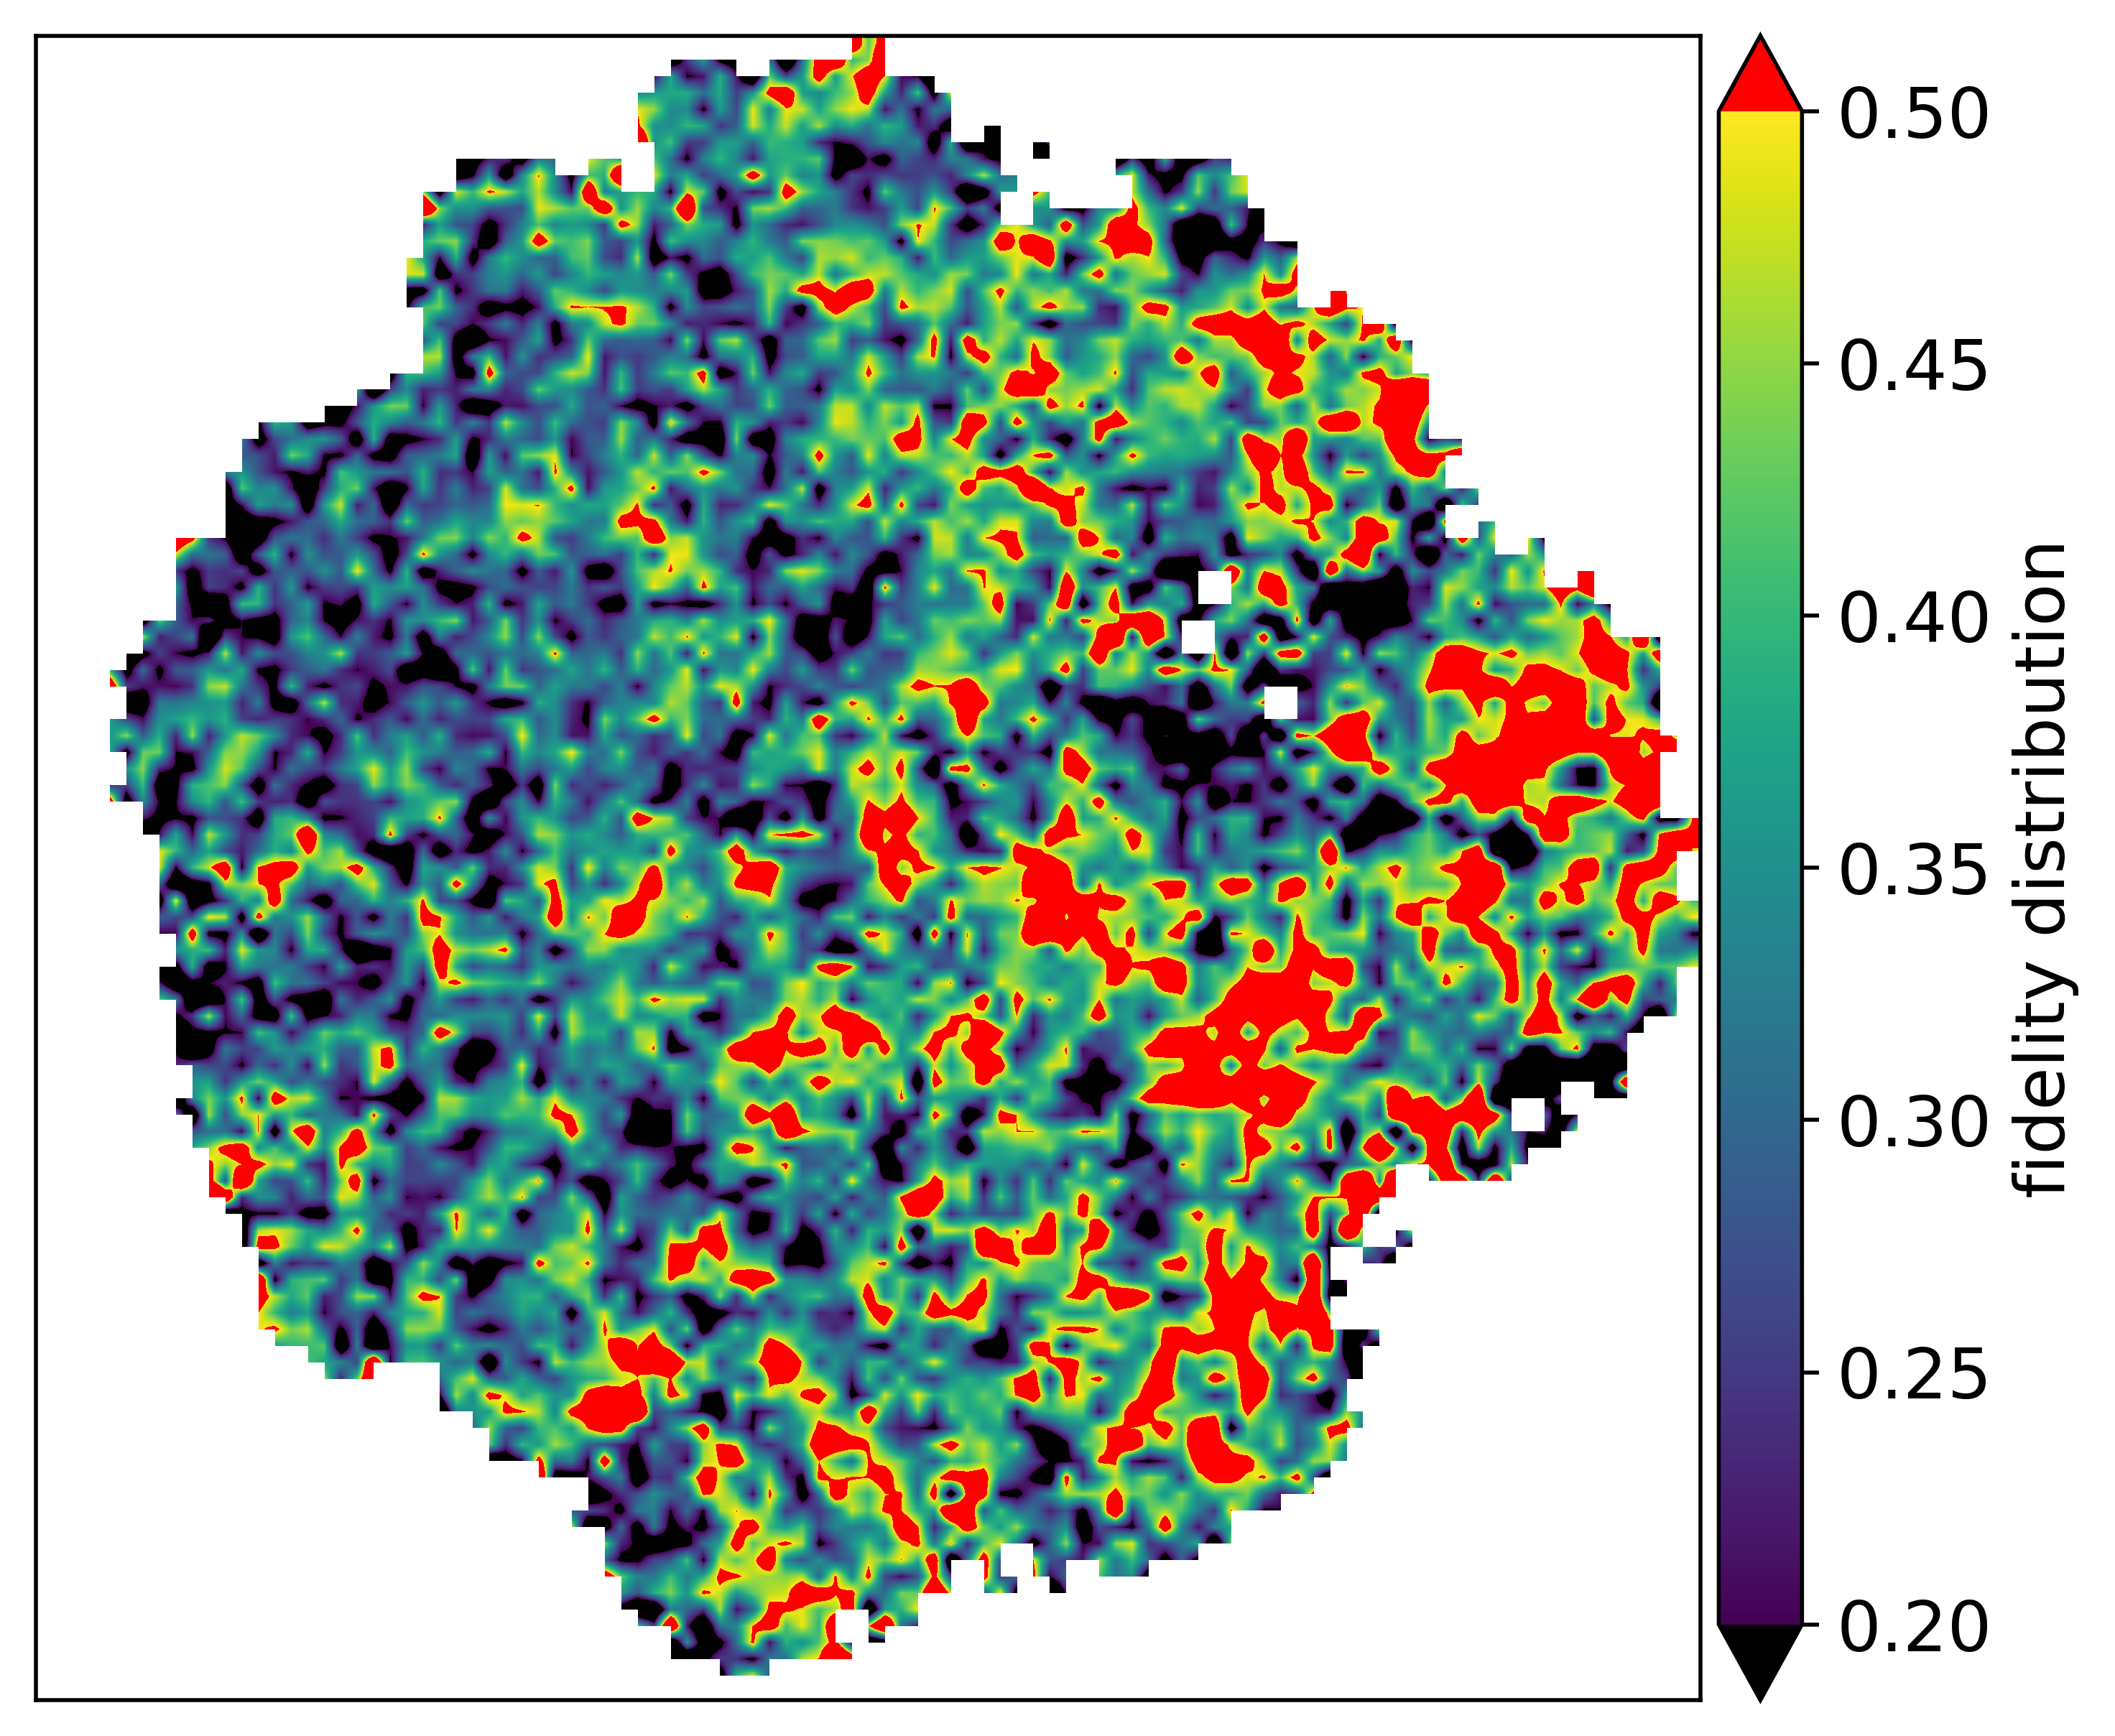
\includegraphics[width=\textwidth]{images/tsqe/fidelity-model-circuits_4_qubits_quantum_arch2vec_full_embedding_full_embedding_smooth.png}
        \caption{t-SNE$_4$ Fidelity}
        \label{fig:t-SNE4 Prev}
    \end{subfigure}
    \begin{subfigure}{0.23\textwidth}
        \centering
        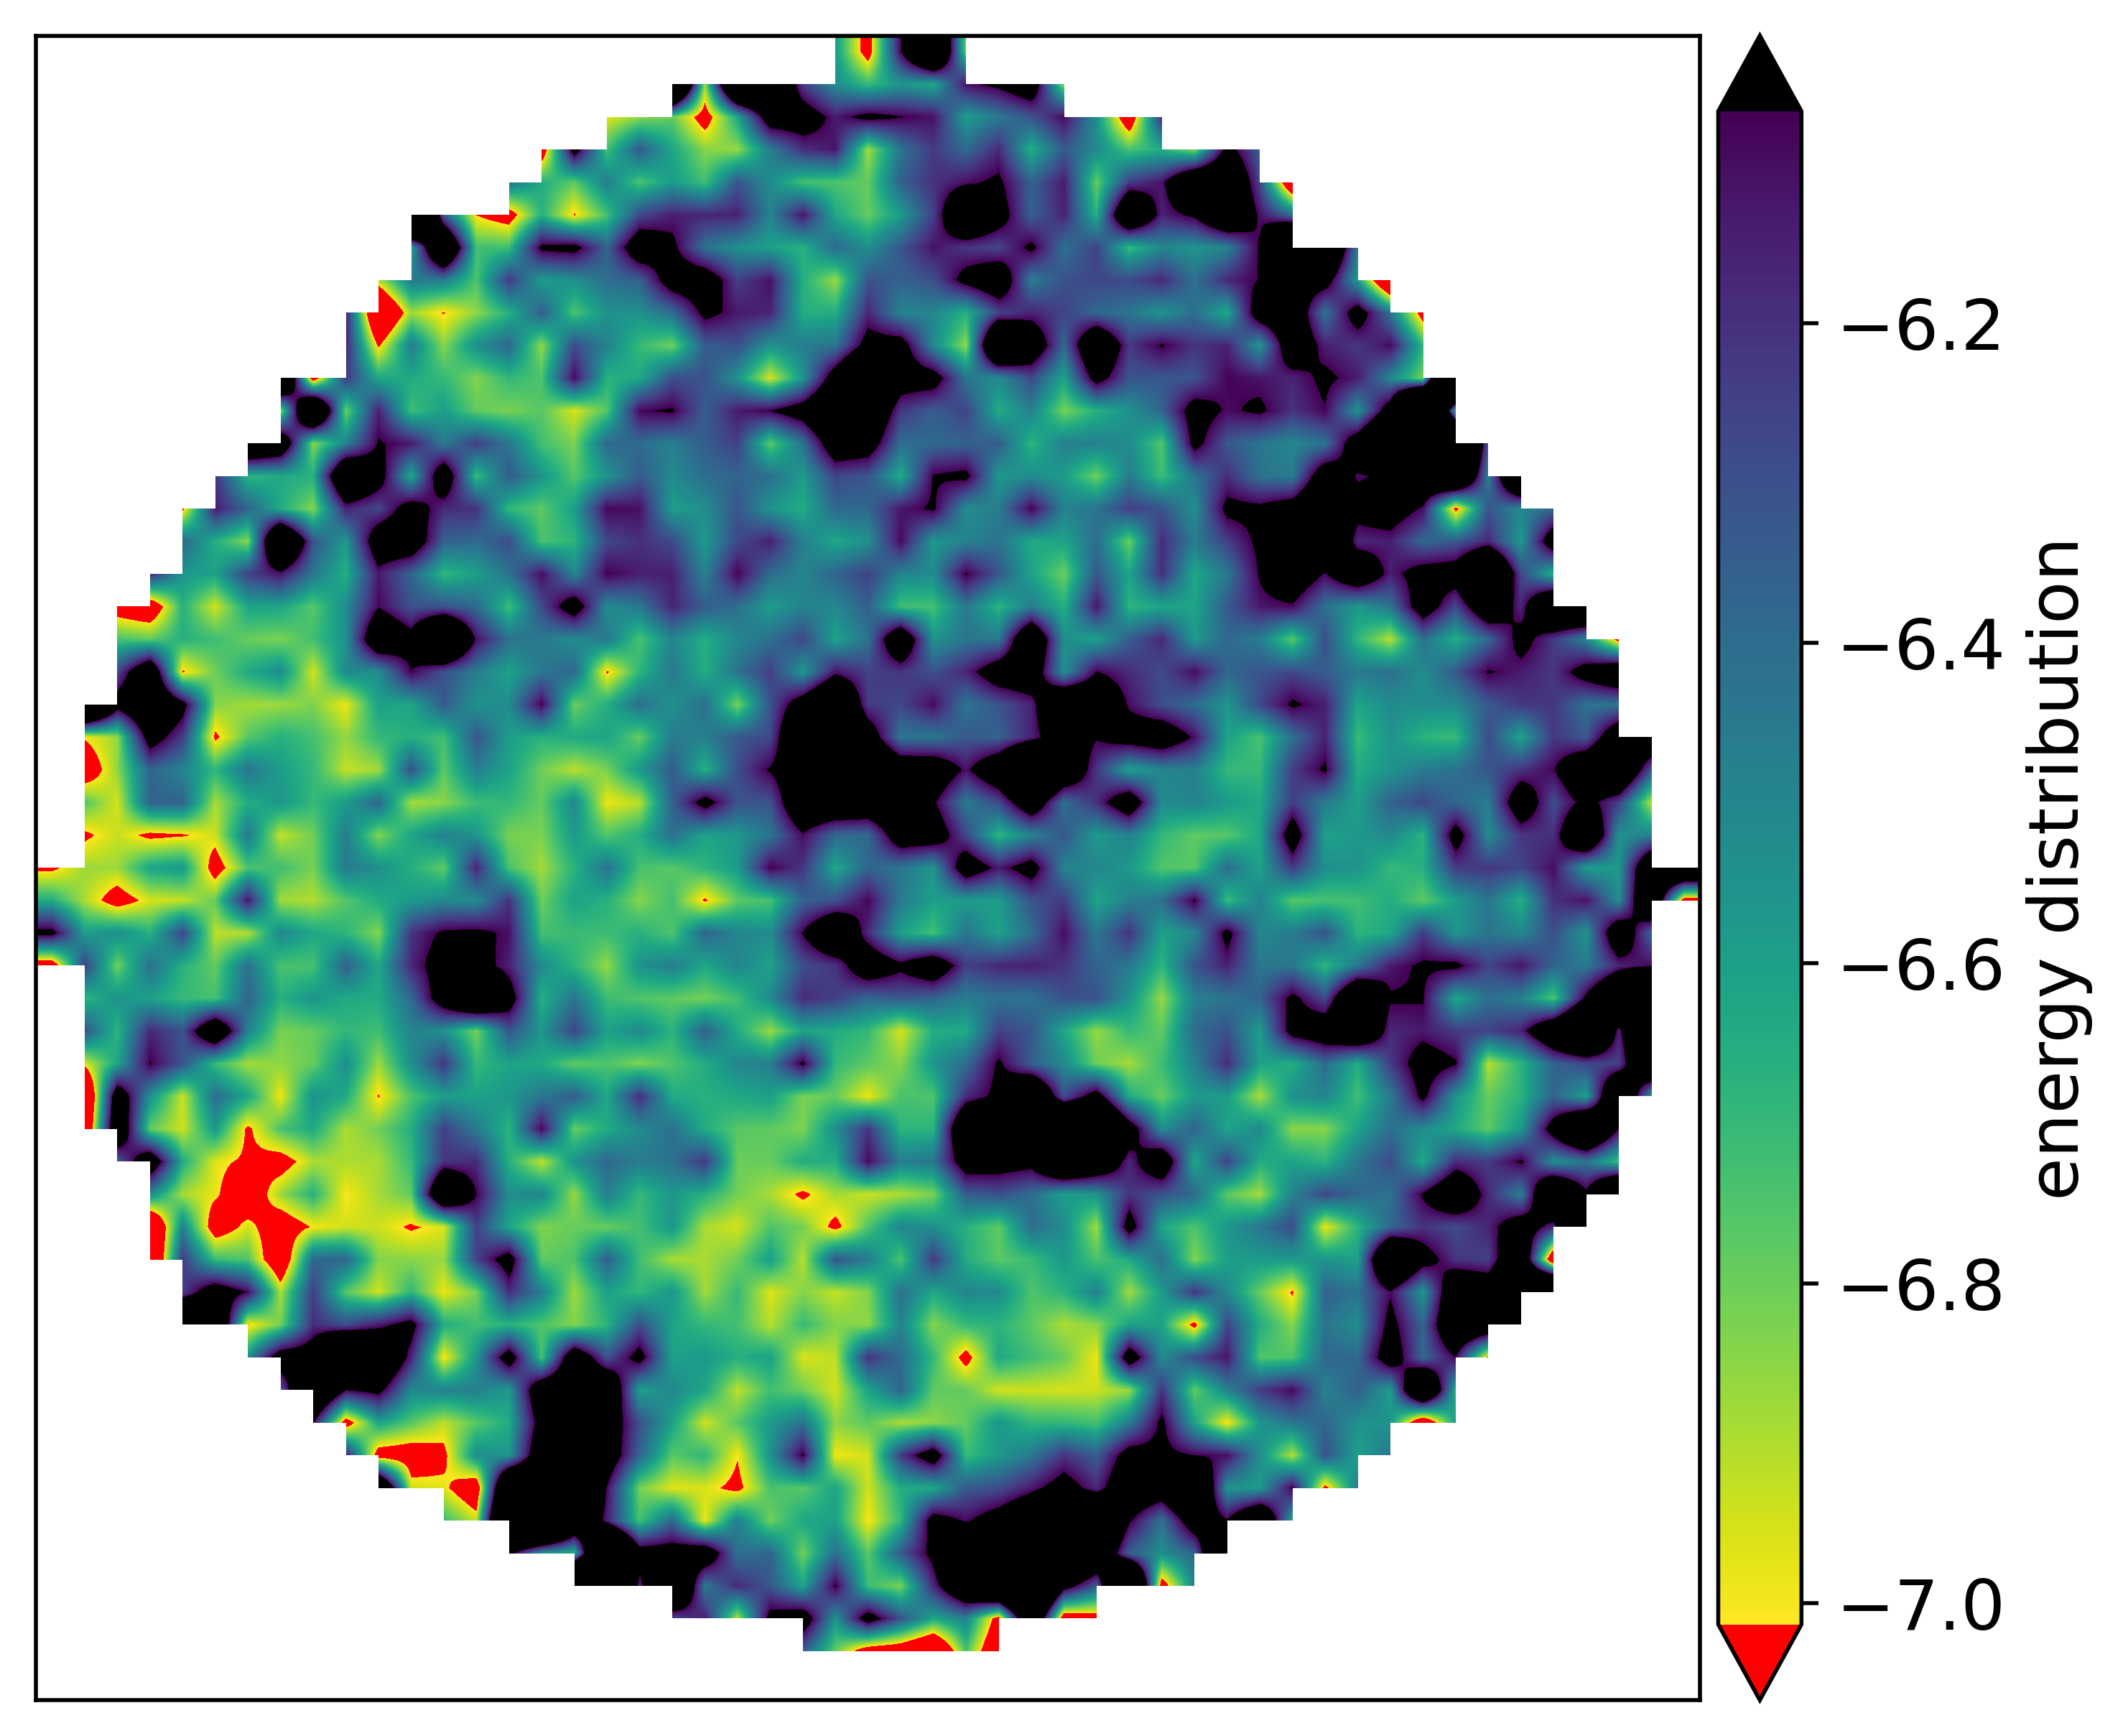
\includegraphics[width=\textwidth]{images/tsqe/vqe-model-circuits_12_qubits_quantum_arch2vec_full_embedding_full_embedding_smooth.png}
        \caption{t-SNE$_{12}$ QC$_{LiH}$}
        \label{fig:t-SNE-12}
    \end{subfigure}

    % Thrid row
    \begin{subfigure}{0.14\textwidth}
        \centering
        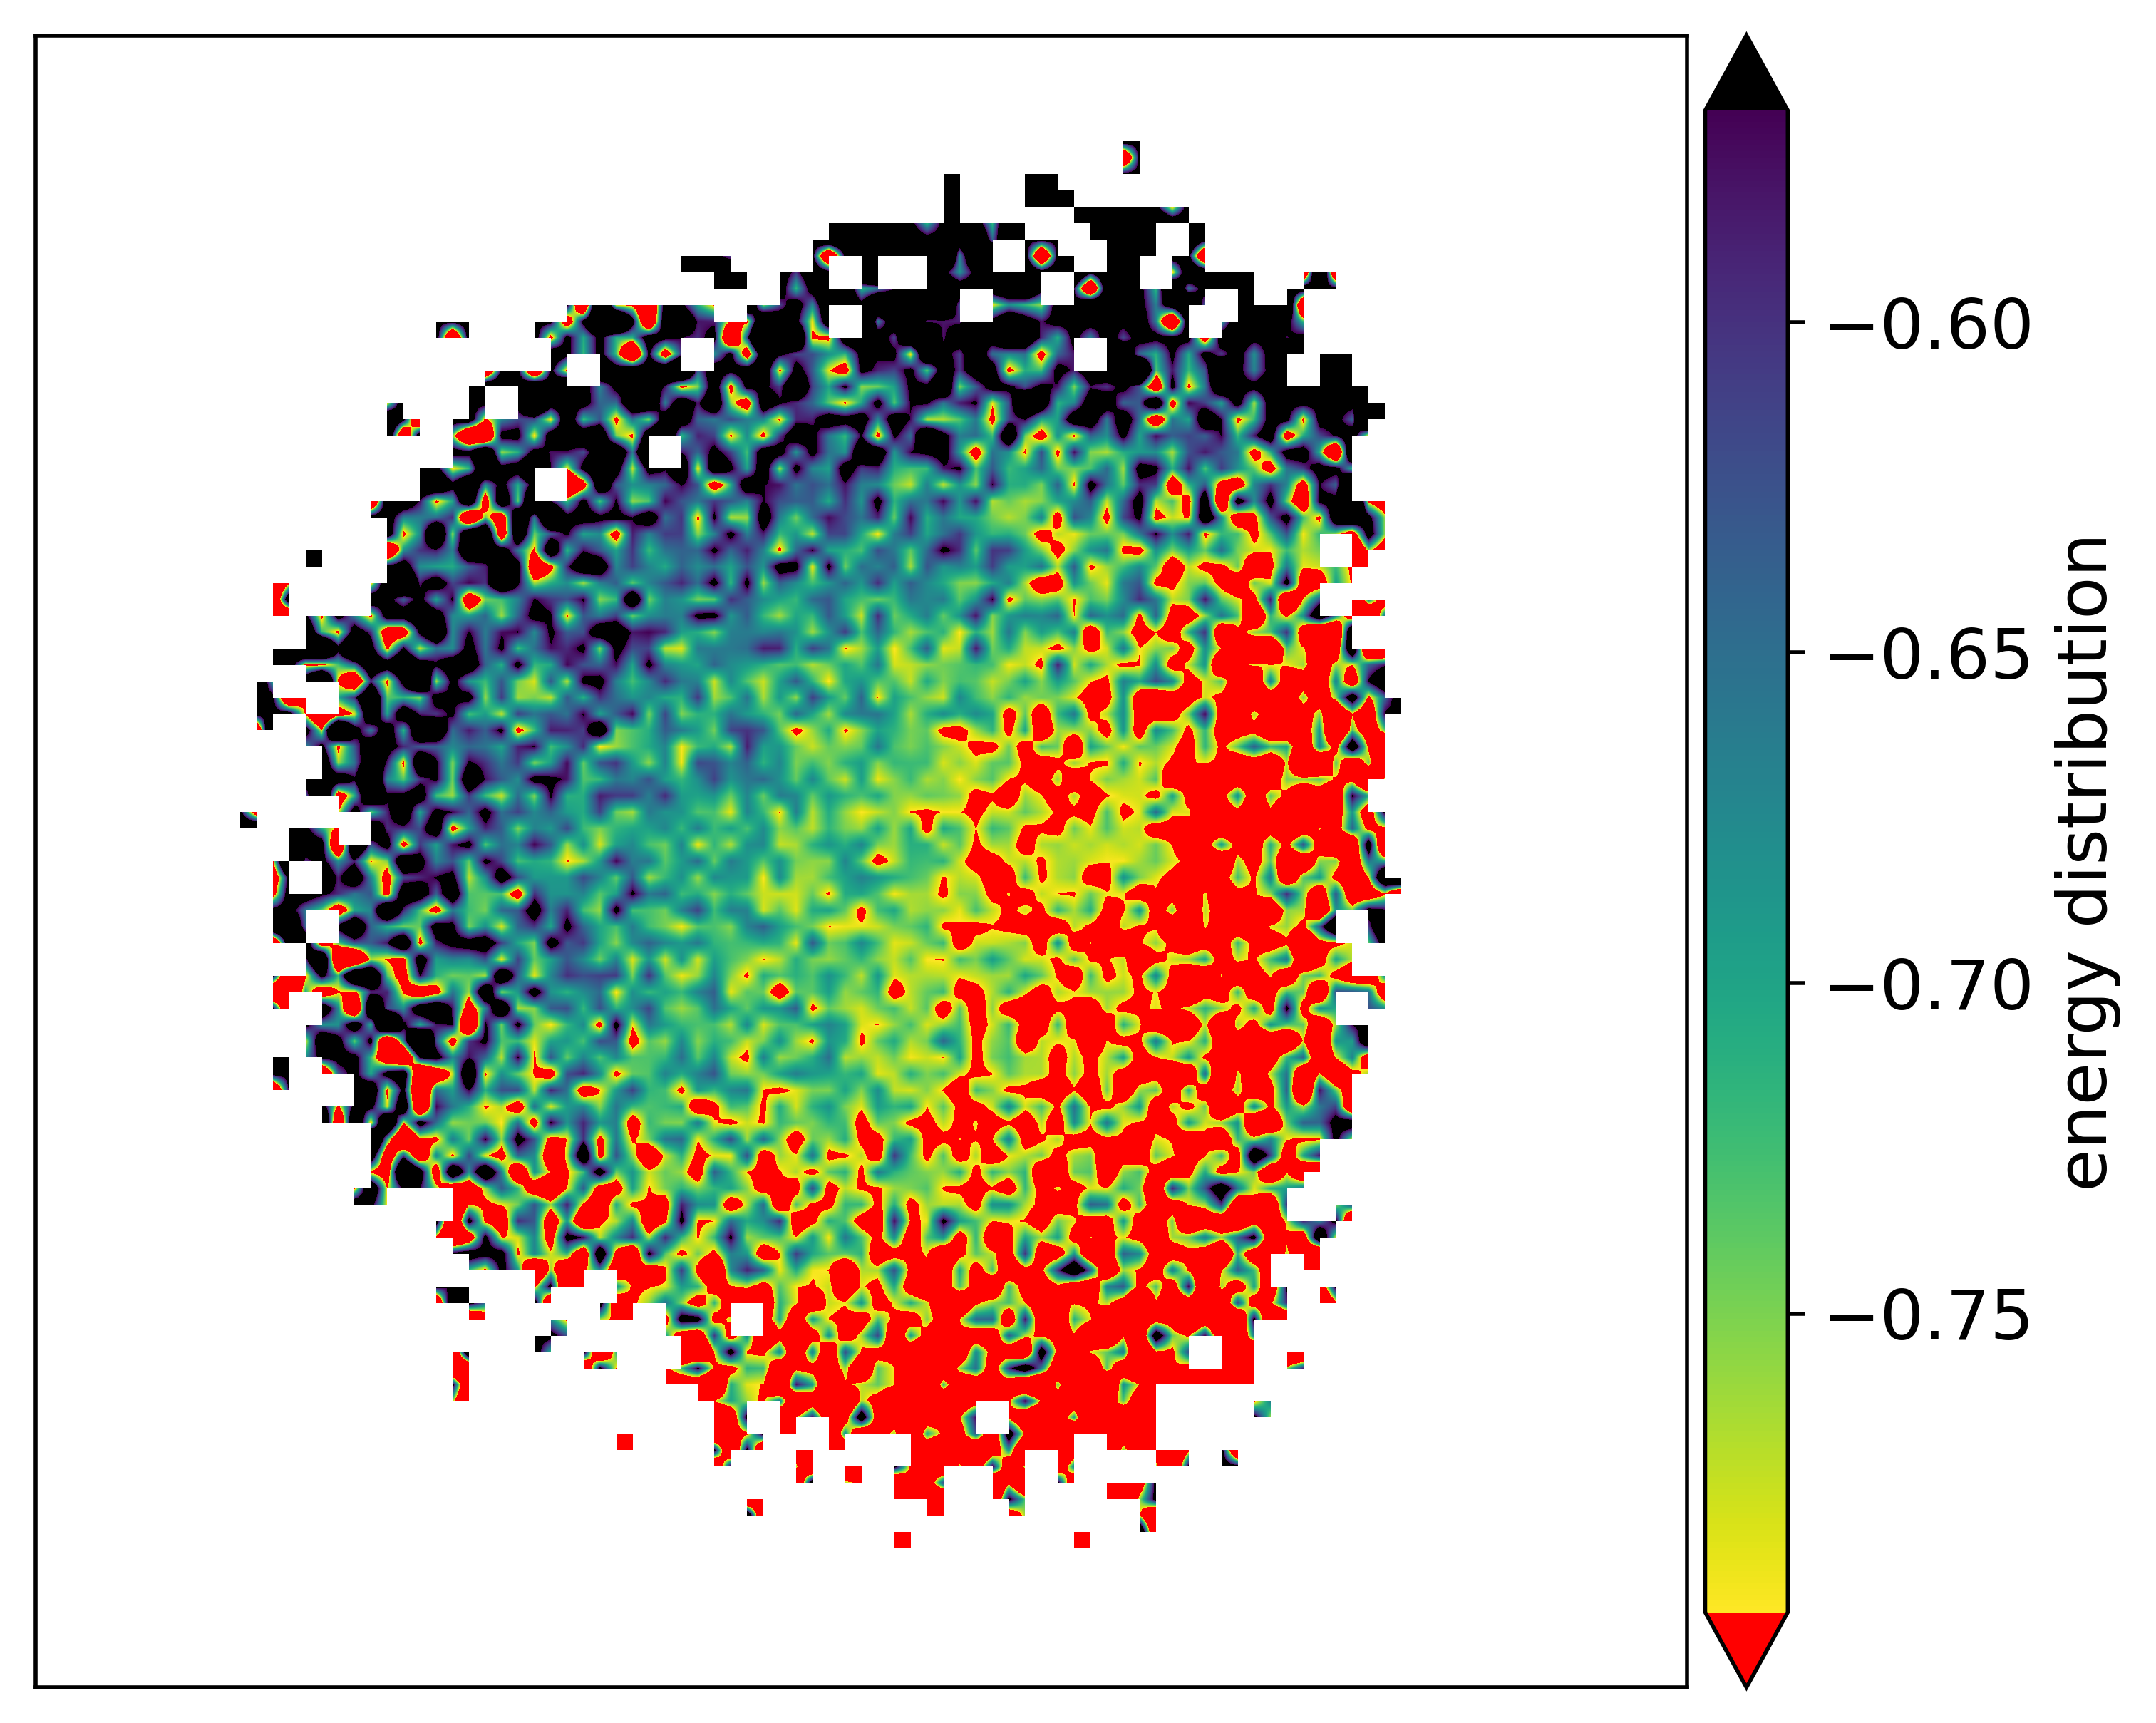
\includegraphics[width=\textwidth]{images/vqe-model-circuits_4_qubits_gsqas_full_embedding_full_embedding_smooth.png}
        \caption{PCA$_4$ Q}
        \label{fig:Prev PCA-4 QC}
    \end{subfigure}
    %\hspace{0.02\textwidth}
    \begin{subfigure}{0.14\textwidth}
        \centering
        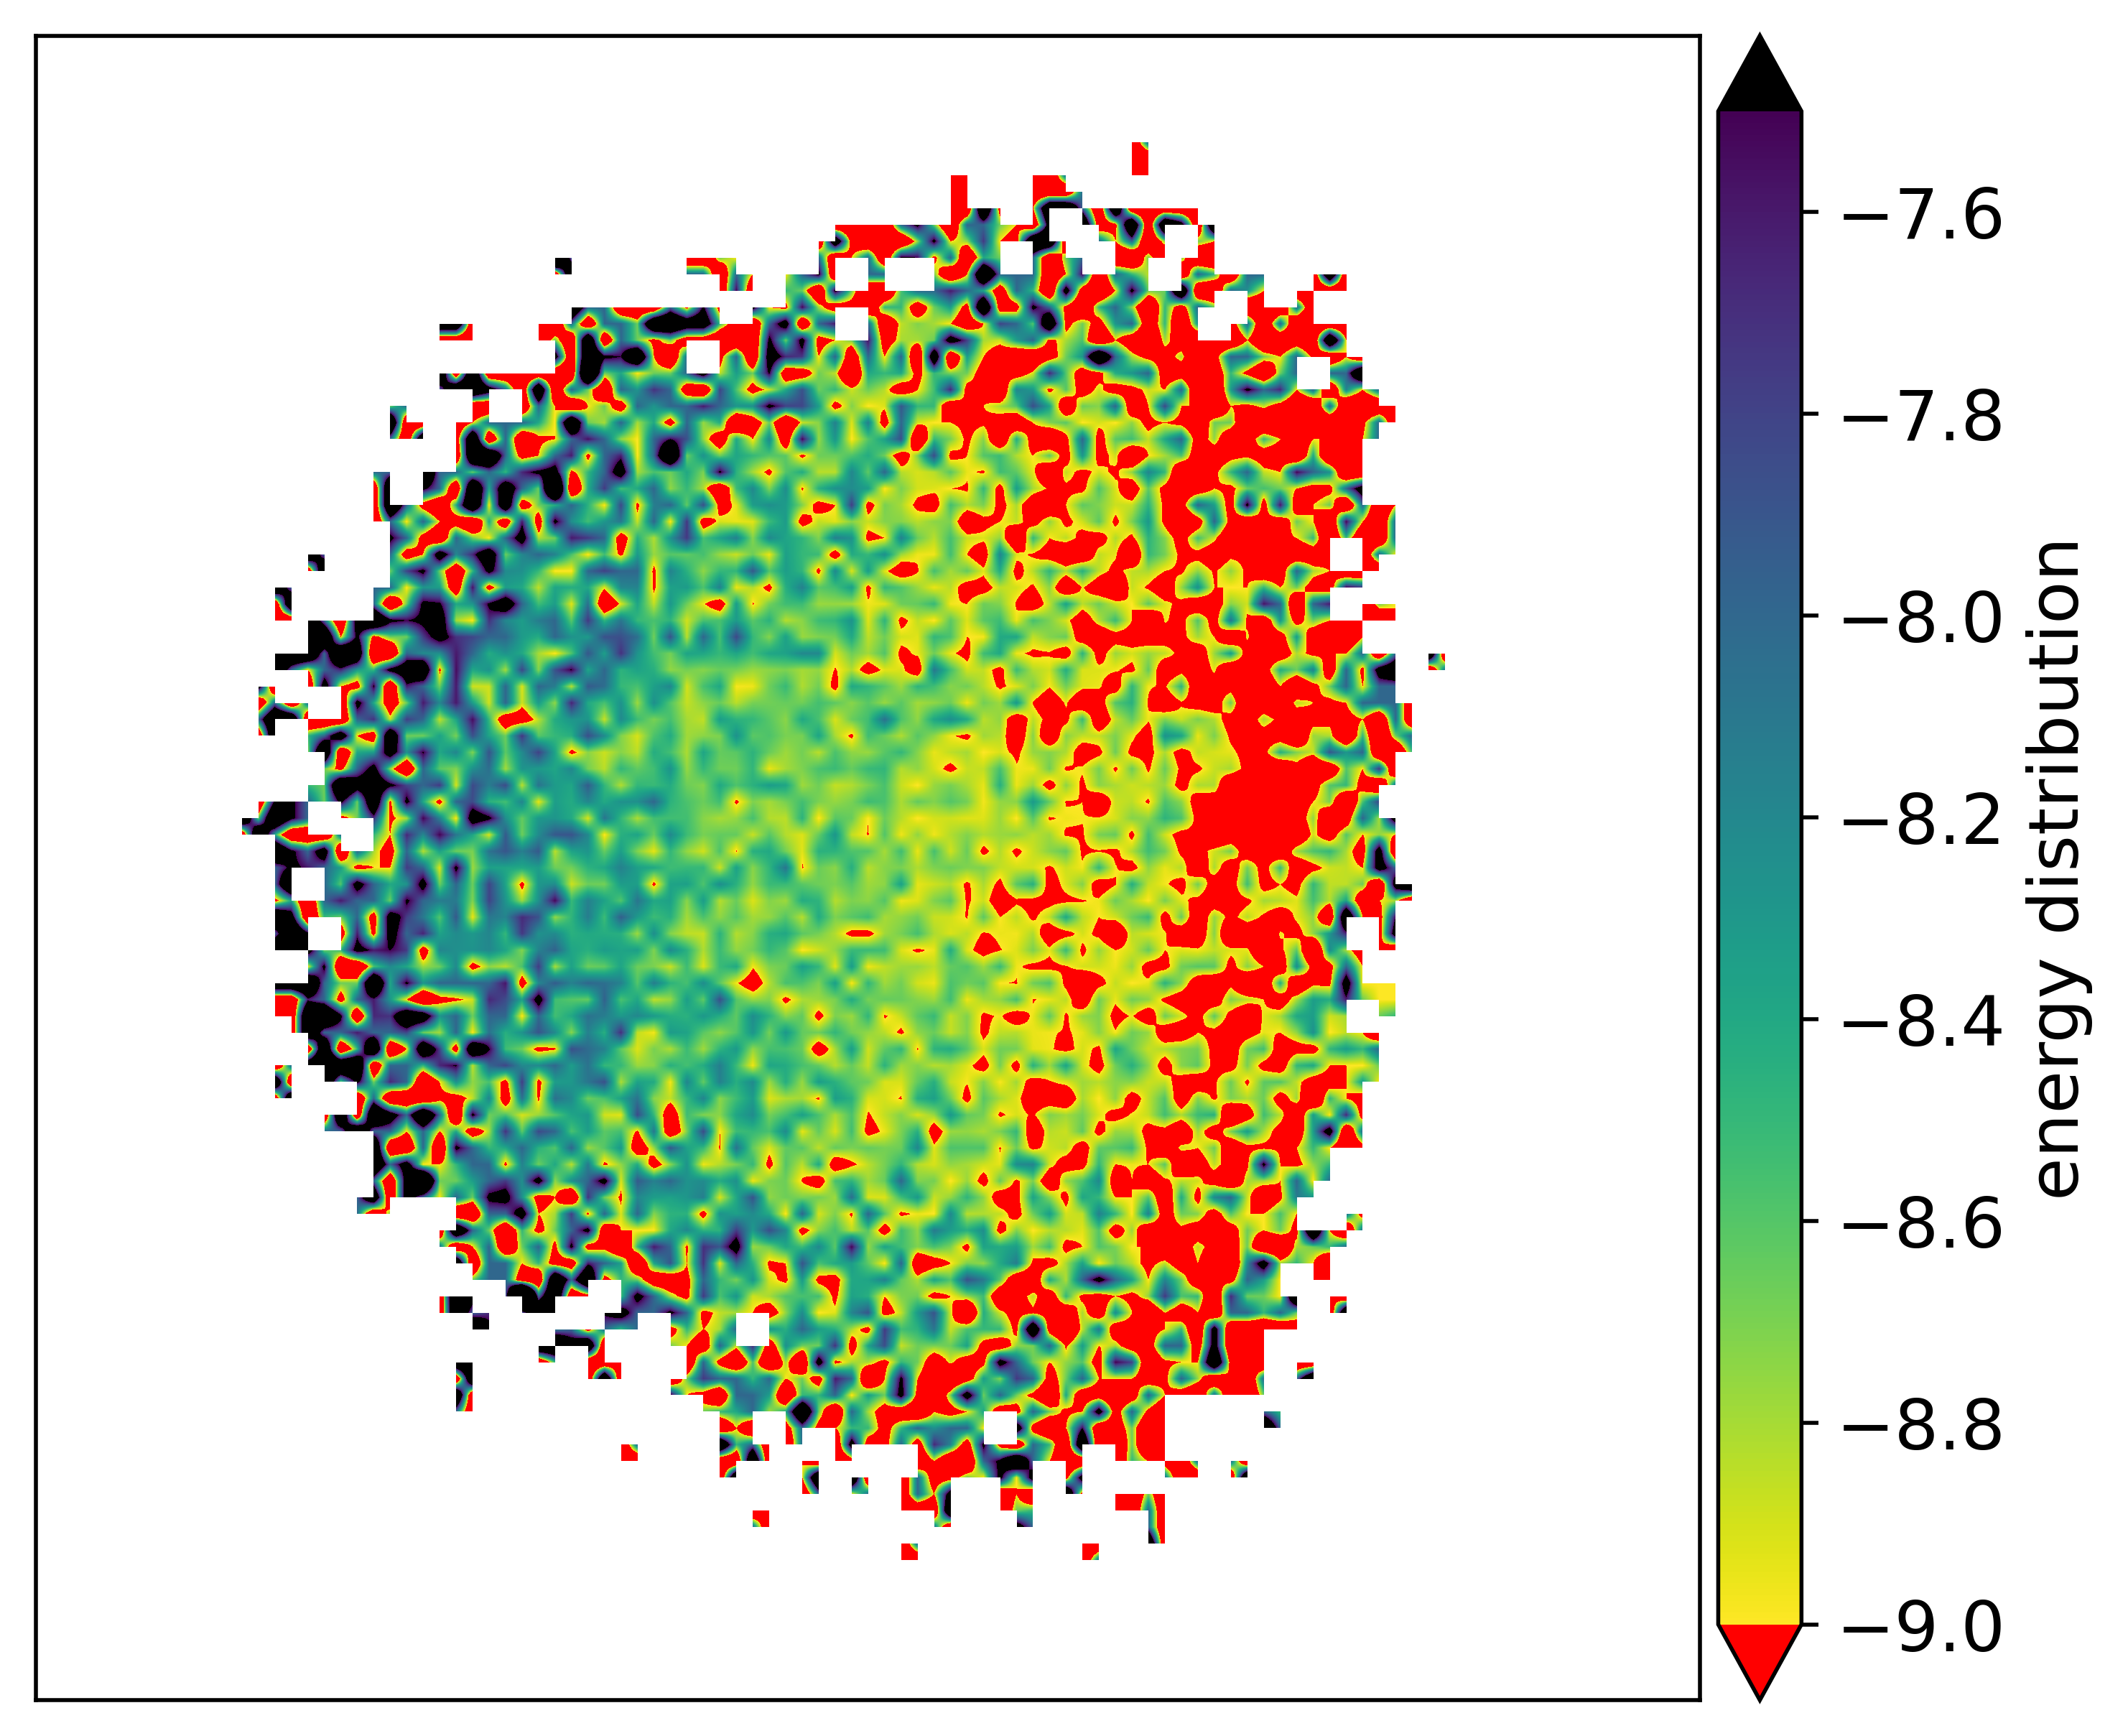
\includegraphics[width=\textwidth]{images/maxcut-model-circuits_4_qubits_gsqas_full_embedding_full_embedding_smooth.png}
        \caption{PCA$_4$ M}
        \label{fig:Prev PCA-4 Maxcut}
    \end{subfigure}
    \begin{subfigure}{0.14\textwidth}
        \centering
        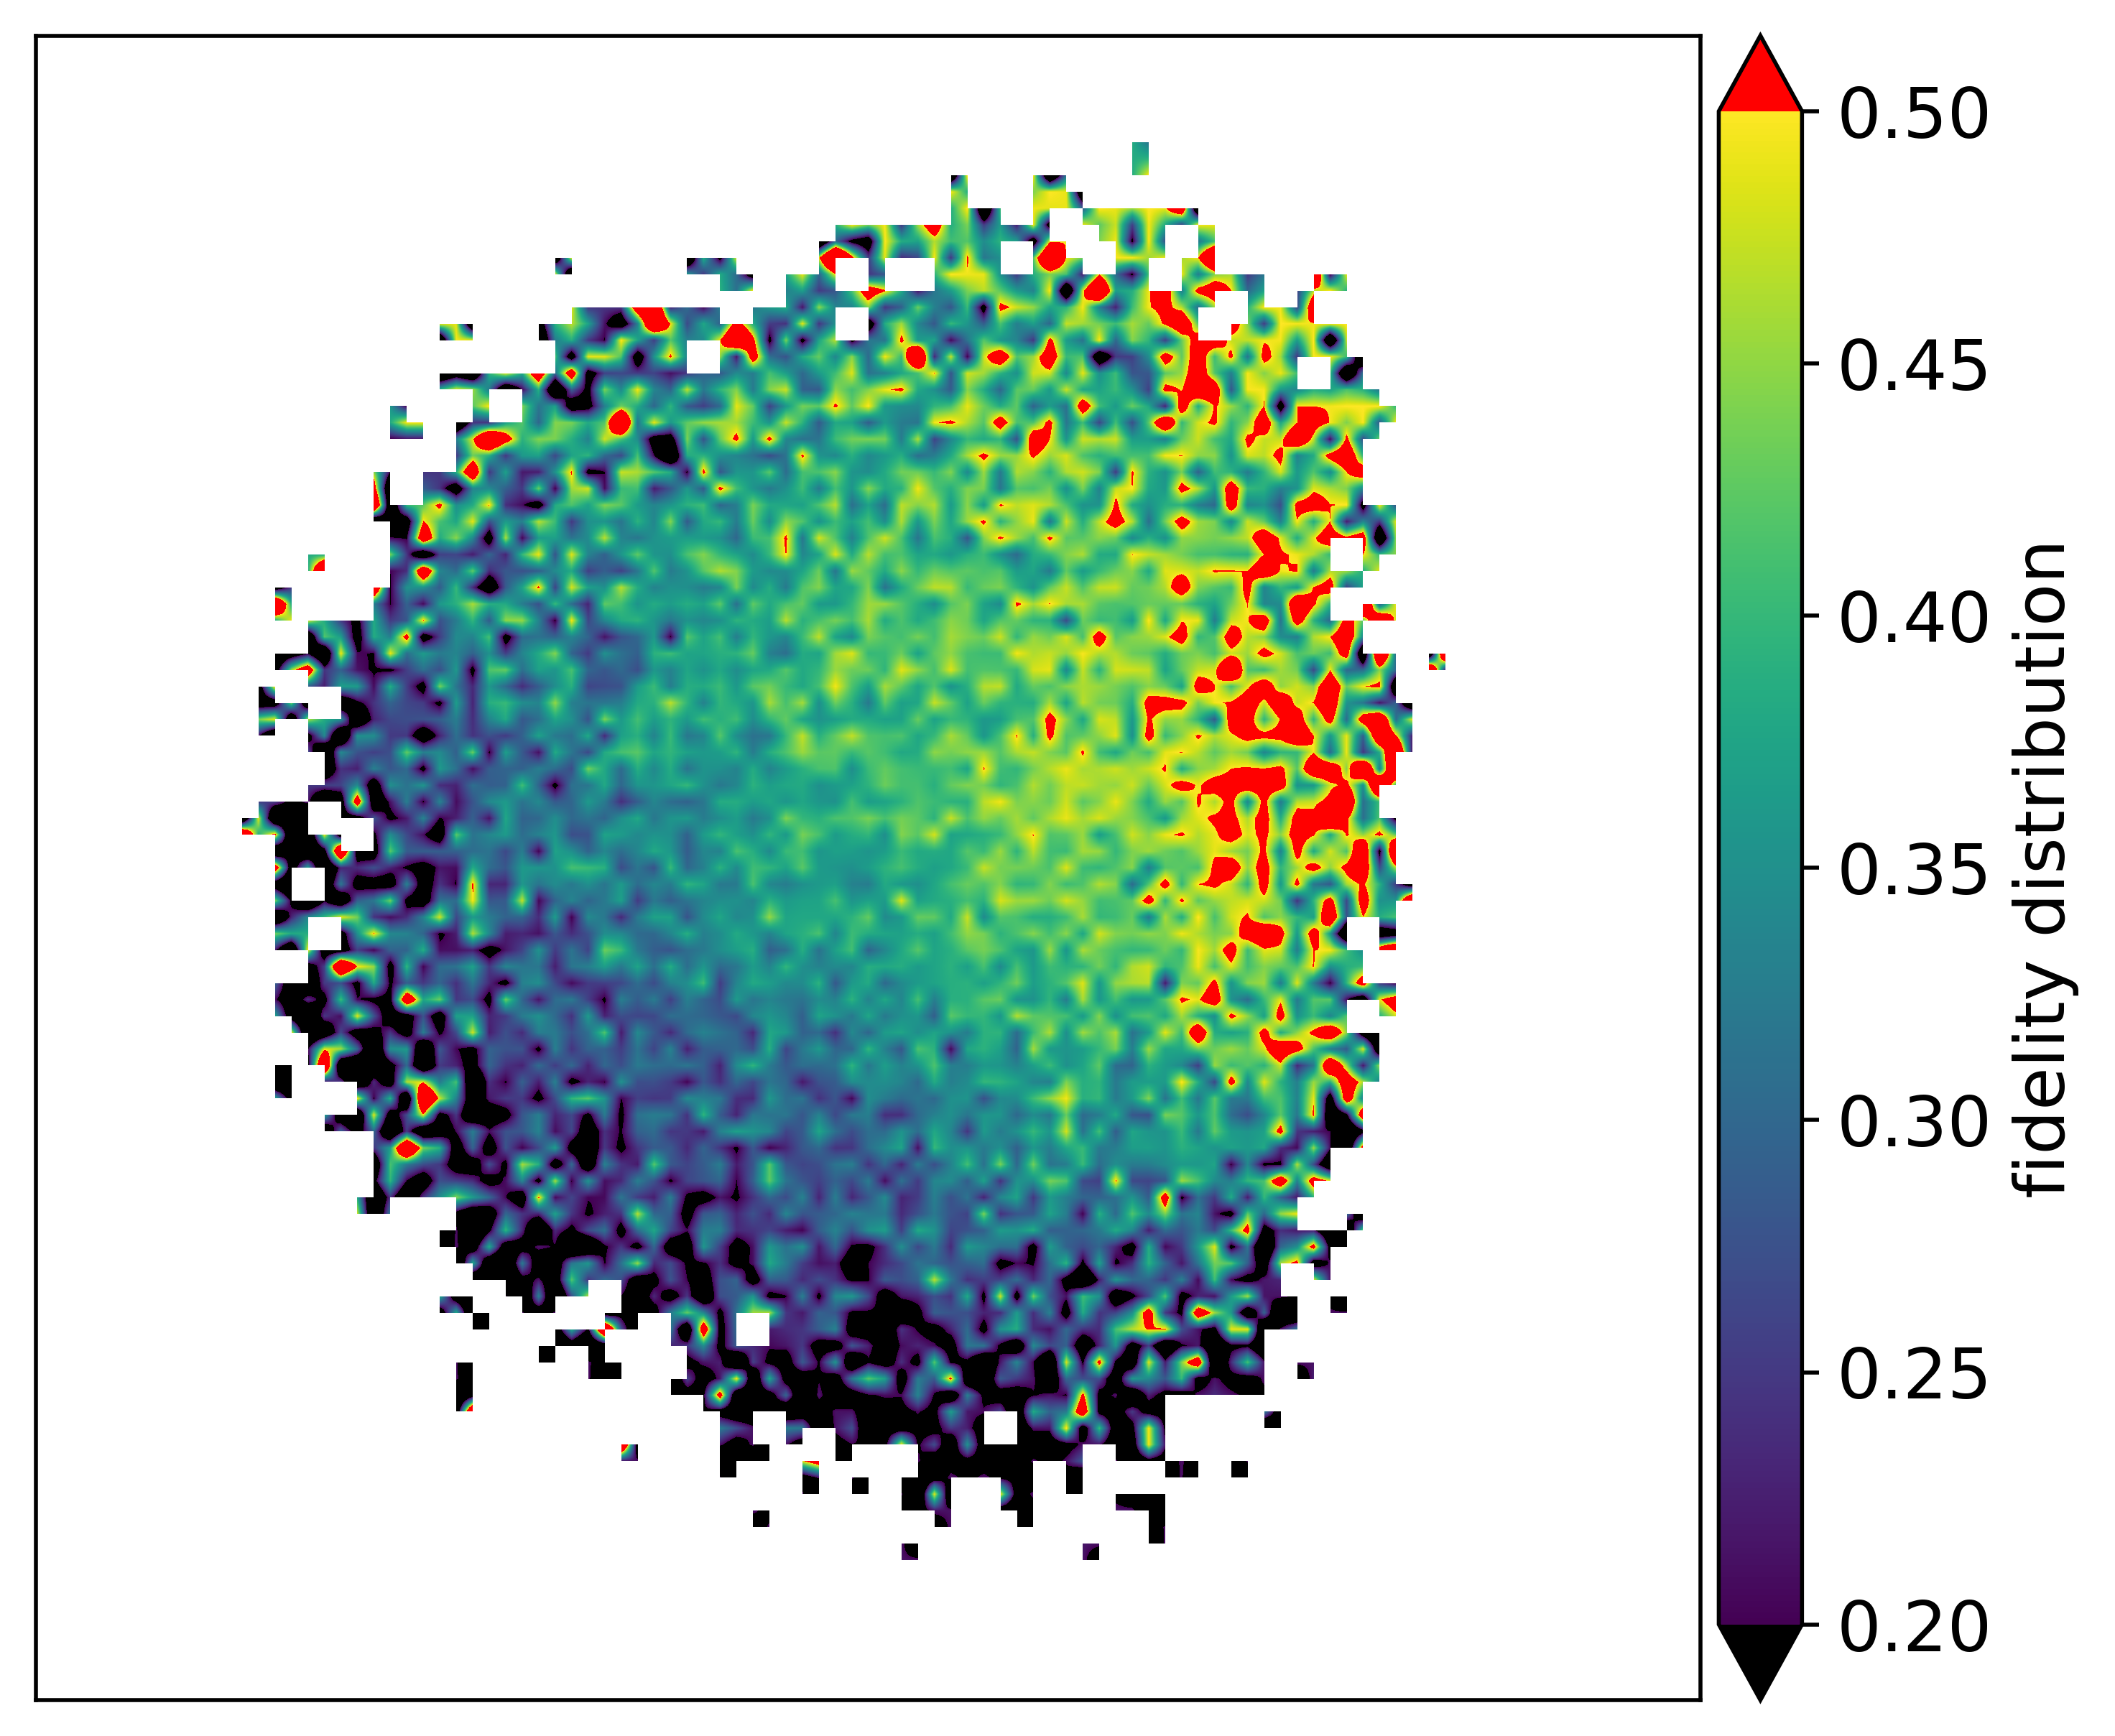
\includegraphics[width=\textwidth]{images/fidelity-model-circuits_4_qubits_gsqas_full_embedding_full_embedding_smooth.png}
        \caption{PCA$_4$ F}
        \label{fig:Prev PCA-4 Fidelity}
    \end{subfigure}
    \begin{subfigure}{0.14\textwidth}
        \centering
        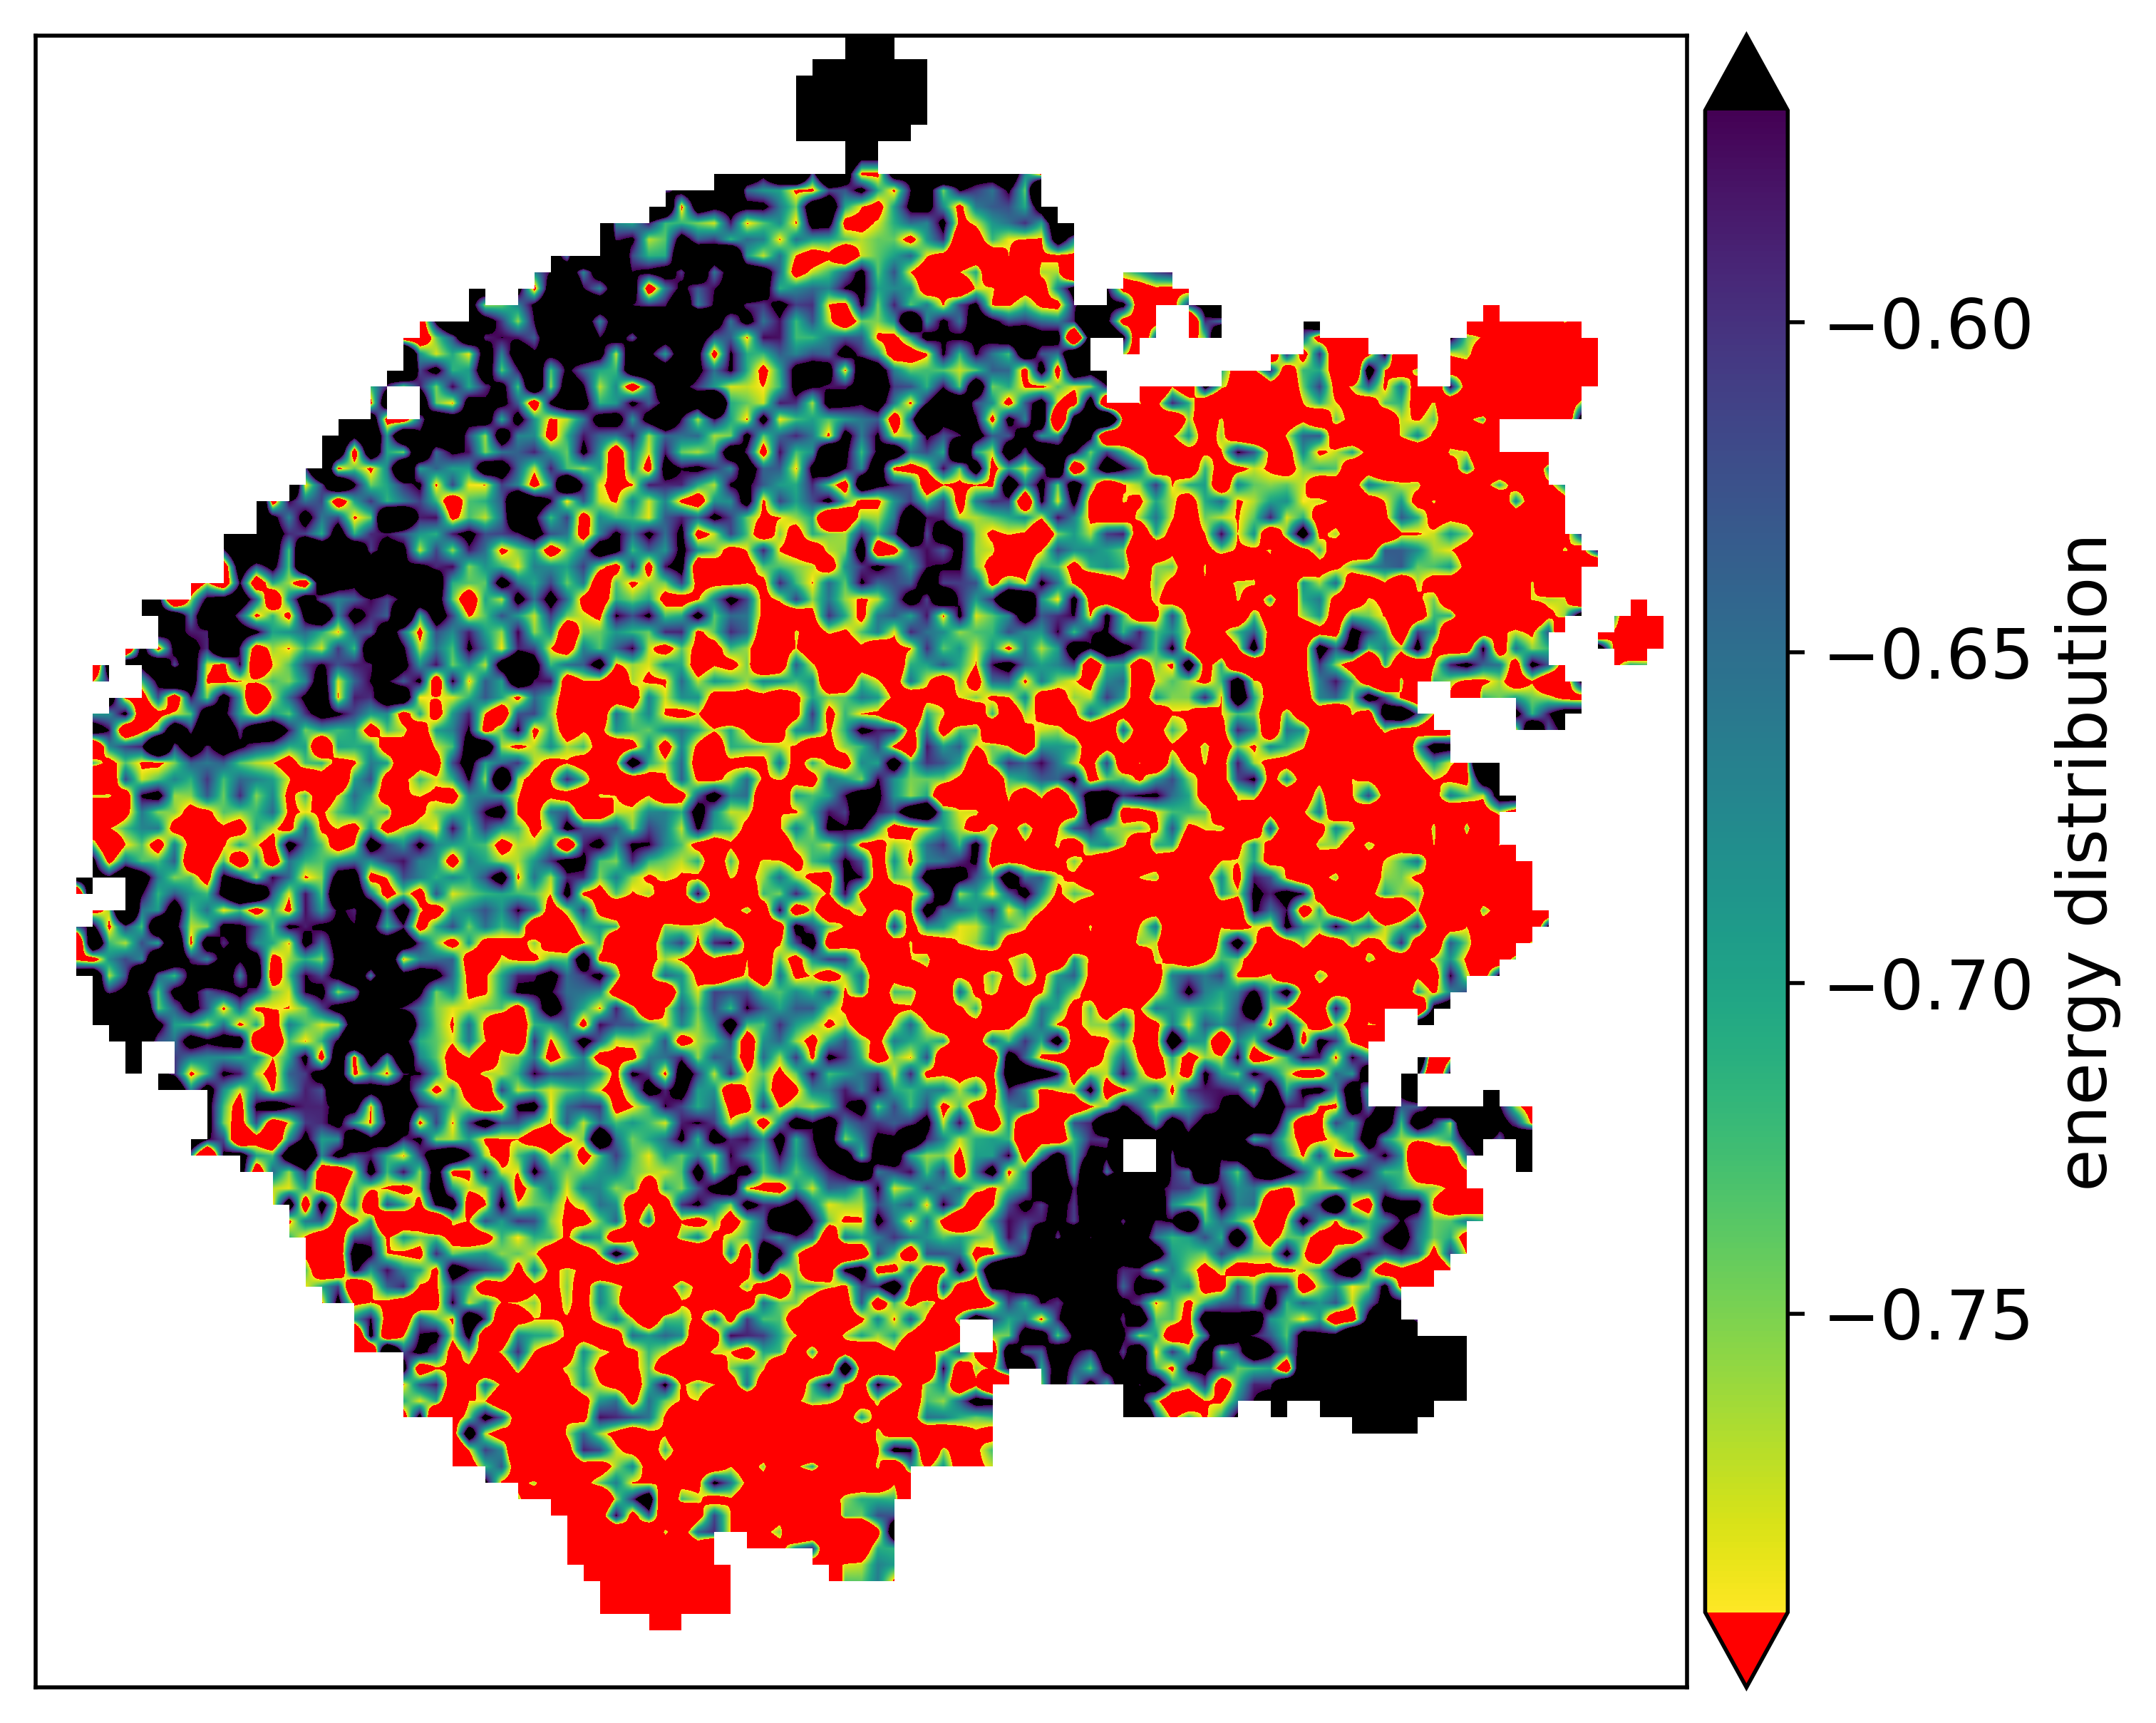
\includegraphics[width=\textwidth]{images/tsqe/vqe-model-circuits_4_qubits_gsqas_full_embedding_full_embedding_smooth.png}
        \caption{t-SNE$_4$ Q}
        \label{fig: Prev t-SNE-4 vqe}
    \end{subfigure}
    \begin{subfigure}{0.14\textwidth}
        \centering
        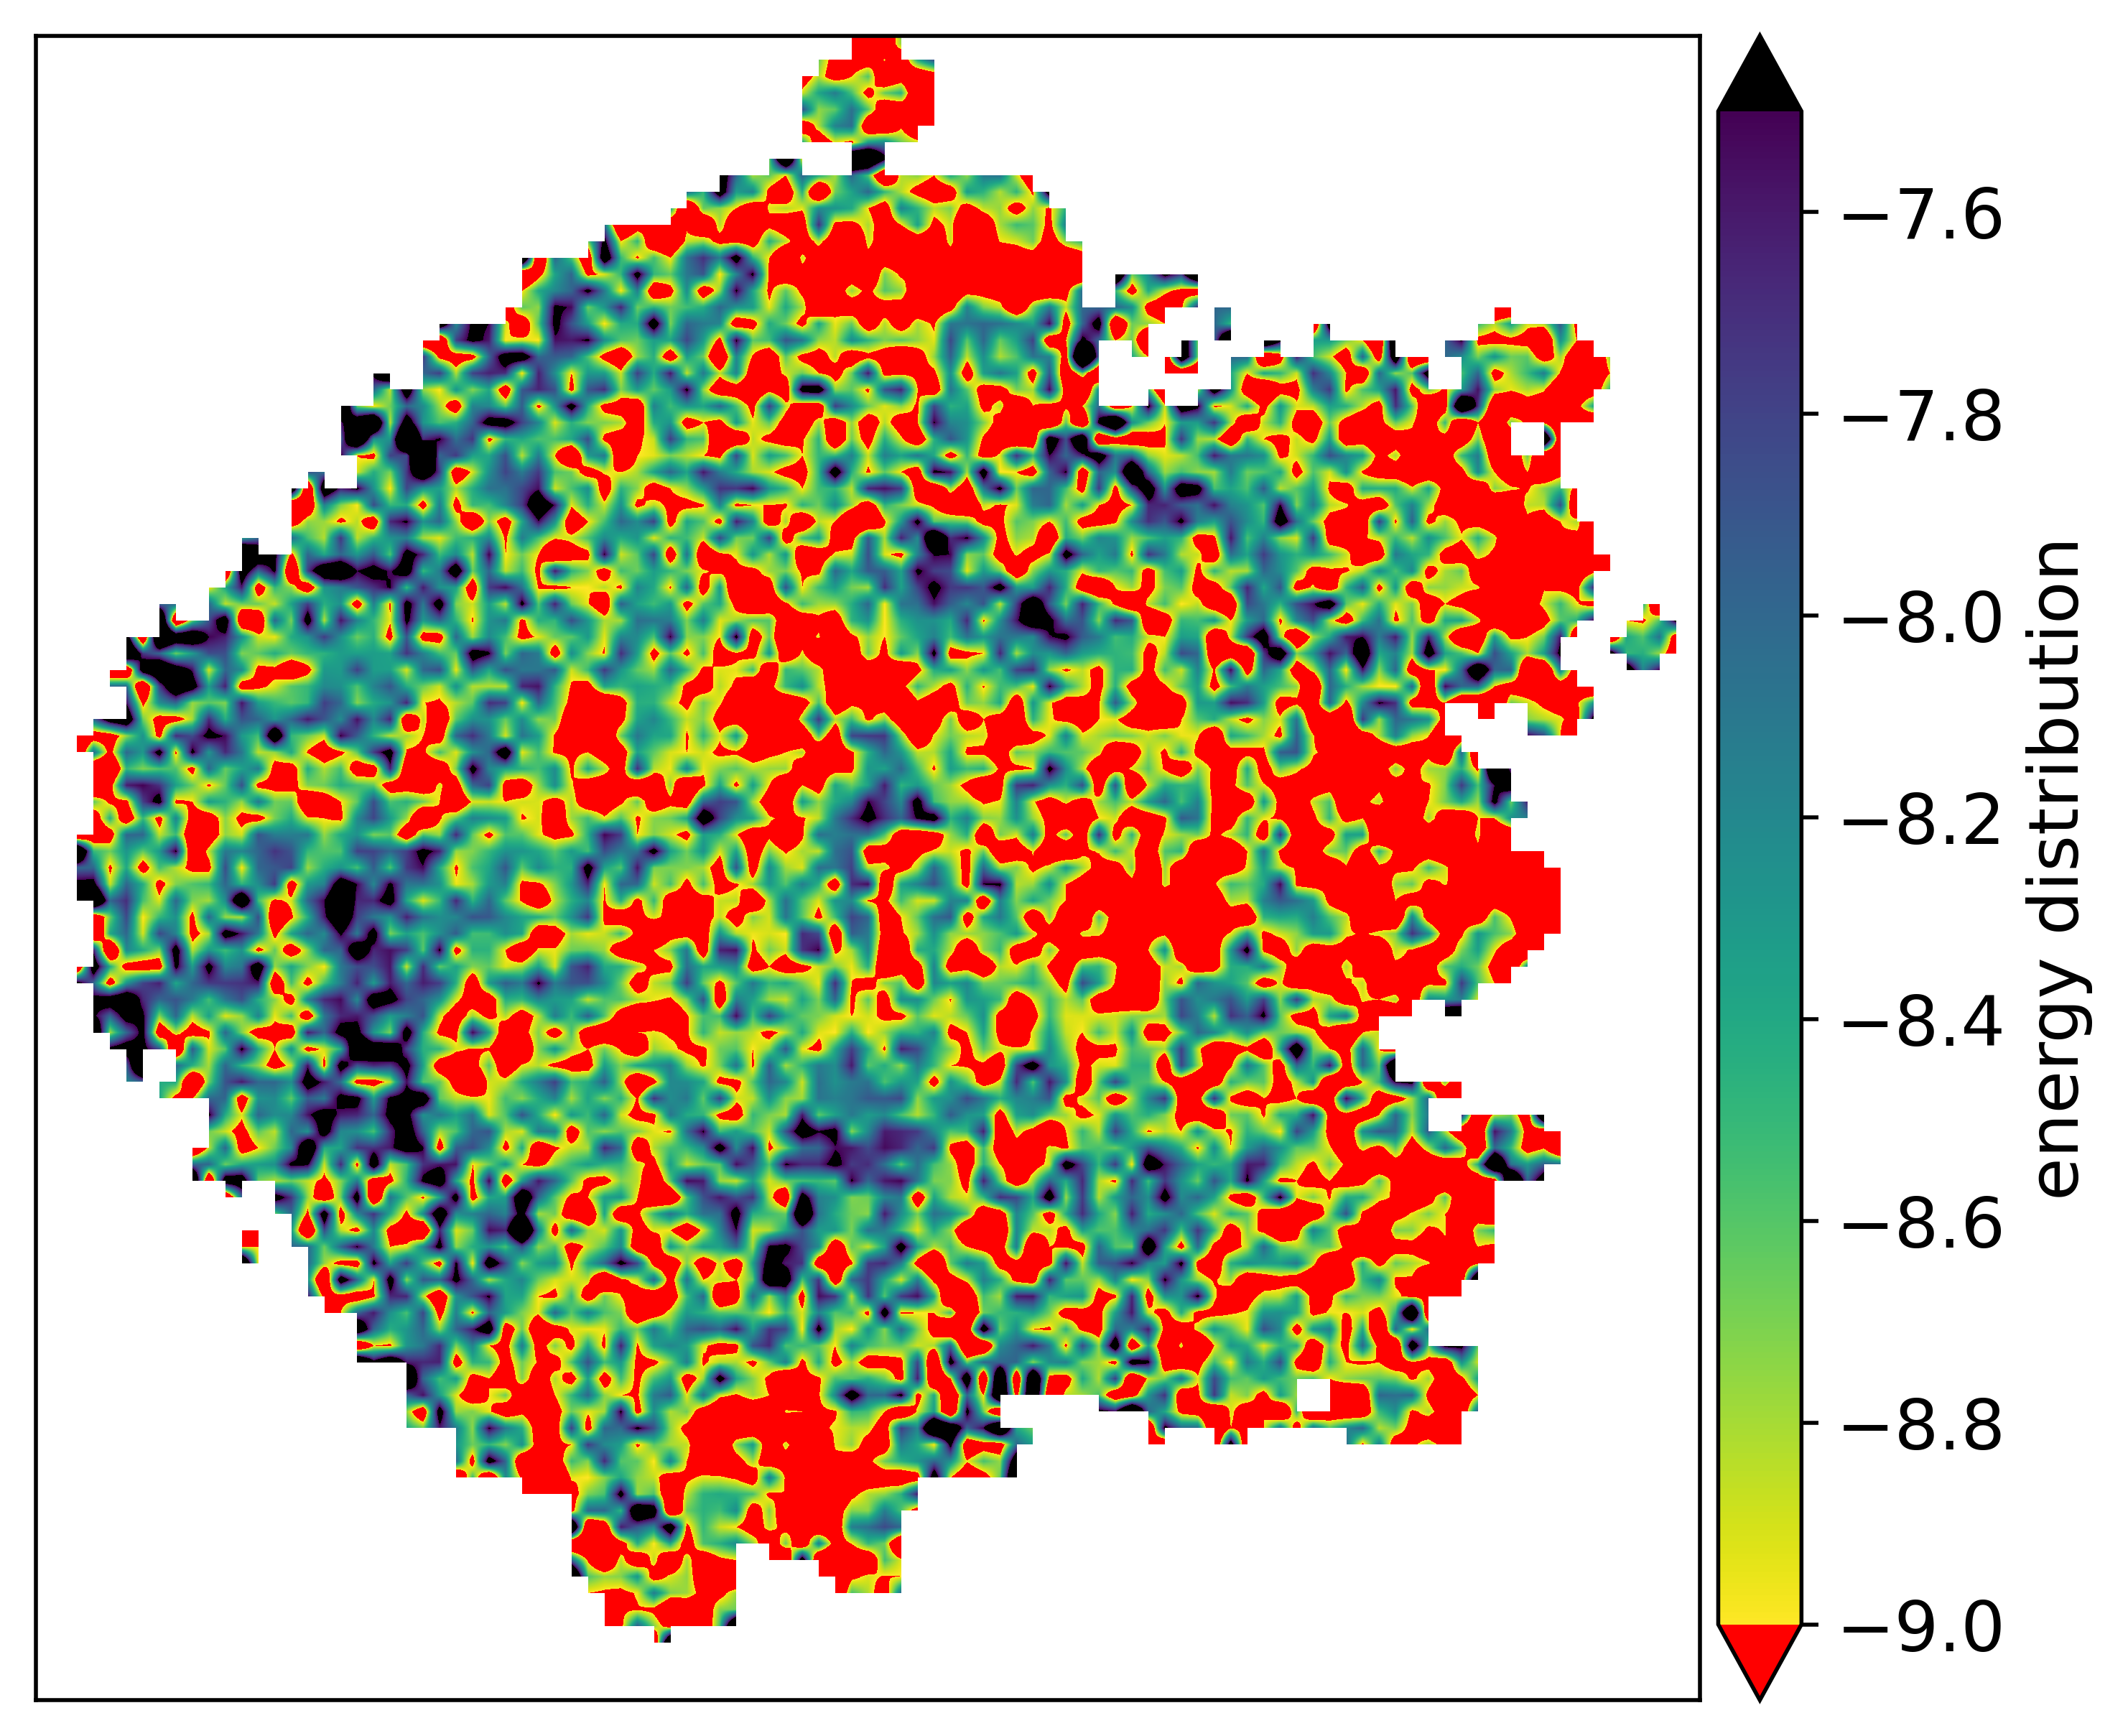
\includegraphics[width=\textwidth]{images/tsqe/maxcut-model-circuits_4_qubits_gsqas_full_embedding_full_embedding_smooth.png}
        \caption{t-SNE$_4$ M}
        \label{fig:Prev t-SNE 4 maxcut}
    \end{subfigure}
    \begin{subfigure}{0.14\textwidth}
        \centering
        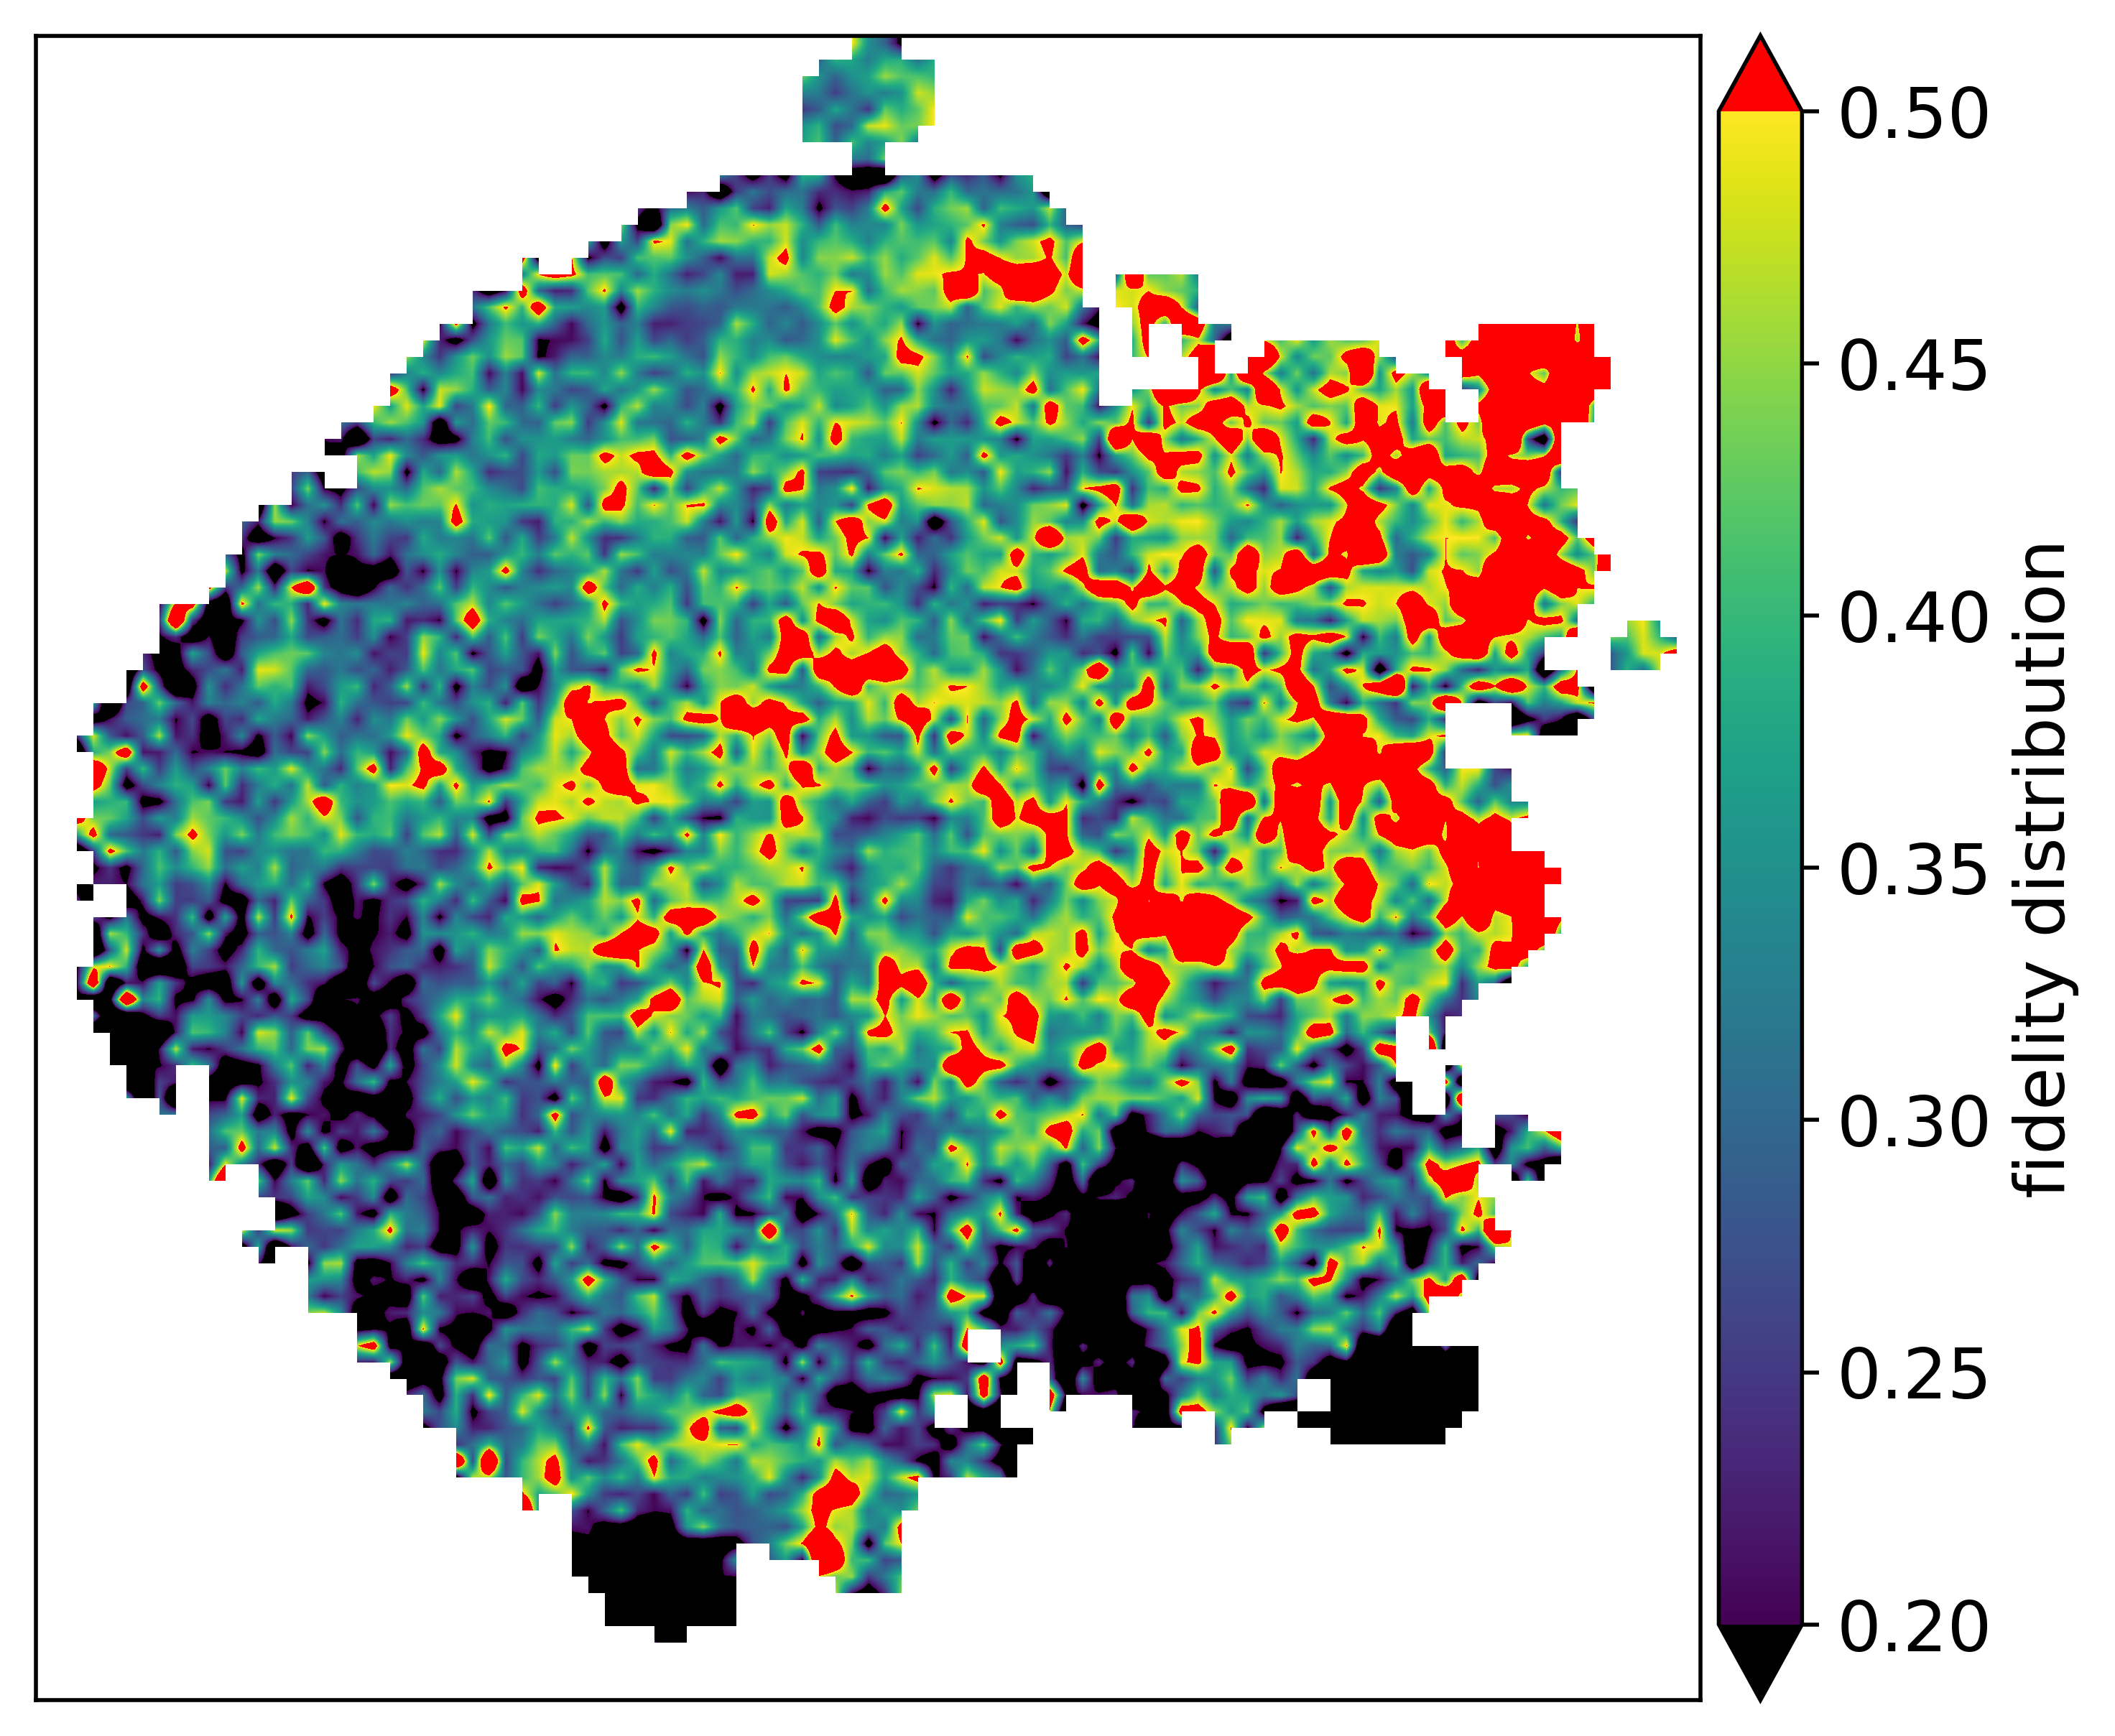
\includegraphics[width=\textwidth]{images/tsqe/fidelity-model-circuits_4_qubits_gsqas_full_embedding_full_embedding_smooth.png}
        \caption{t-SNE$_4$ F}
        \label{fig:prev t-sne4 fidelity}
    \end{subfigure}
    
    \caption{The 2D smooth visualizations of the latent representations for the 4- and 12-qubit cases, using PCA and t-SNE. The color encoding reflects the achieved energy of 100,000 randomly generated circuits. These latent representations are introduced for three QML tasks: Quantum Chemistry, Max-cut, and fidelity. The graphs illustrate the energy or fidelity distribution of the circuits, where red denotes circuits with an energy lower than $-0.80/-0.90/-7.01 , \text{Ha}$ or a fidelity higher than 0.5. The subfigures in the first two rows display the results of our model with KL divergence, while the subfigures at the bottom visualize the 4-qubit latent space using the existing encoding scheme $\mathcal{E}^{GSQAS}$.}
    \label{2D-Visu}
\end{figure}

% \begin{figure}[ht]
% \begin{center}
%     \begin{subfigure}[b]{0.475\textwidth}
%     \centering
%     \includegraphics[width=0.49\textwidth]
%     {images/maxcut-model-circuits_4_qubits_full_embedding_smooth_pca.png}
%     %{pca.drawio.png}%
%     \includegraphics[width=0.49\textwidth]{images/maxcut-model-circuits_4_qubits_wokl_full_embedding_smooth_pca.png} %
%     \caption{PCA result}
%     \label{pca}
%     \end{subfigure}
%     \hspace{0.25cm}
%     \begin{subfigure}[b]{0.475\textwidth}
%     \centering
%     \includegraphics[width=0.49\textwidth]{images/maxcut-model-circuits_4_qubits_full_embedding_smooth_tsne.png}
%     \includegraphics[width=0.49\textwidth]{images/maxcut-model-circuits_4_qubits_wokl_full_embedding_smooth_tsne.png}
%     \caption{t-SNE result} 
%     \label{tsne}
%     \end{subfigure}
%     \caption{The 2D smooth visualization for the latent representation of 4-qubit max-cut with PCA and t-SNE. Color encodes the achieved energy of the randomly generated 100,000 circuits. These graphs show the energy distribution of the 100,000 circuits. Only when the achieved energy is lower than $-9.0 \ Ha$, it is encoded in red. In (a) and (b), the left one is the result of our model with KL divergence and the other is without KL divergence.}
%     \label{embedding}   
% \end{center}
% \end{figure}

\subsection{Quantum Architecture Search (QAS) Performance}
\label{qas_performance}
\textbf{Observation (1):} In Figure \ref{average_reward}, we present the average reward per 100 searches for each experiment. The results show that both the REINFORCE and BO methods effectively learn to navigate the latent representation, leading to noticeable improvements in average reward during the early stages. In contrast, Random Search fails to achieve similar improvements. Furthermore, although the plots indicate slightly higher variance in the average reward for the REINFORCE and BO methods compared to Random Search, their overall average reward is significantly higher than that of Random Search.
\begin{figure}[ht]
\begin{center}
    \begin{subfigure}[b]{0.325\textwidth}
    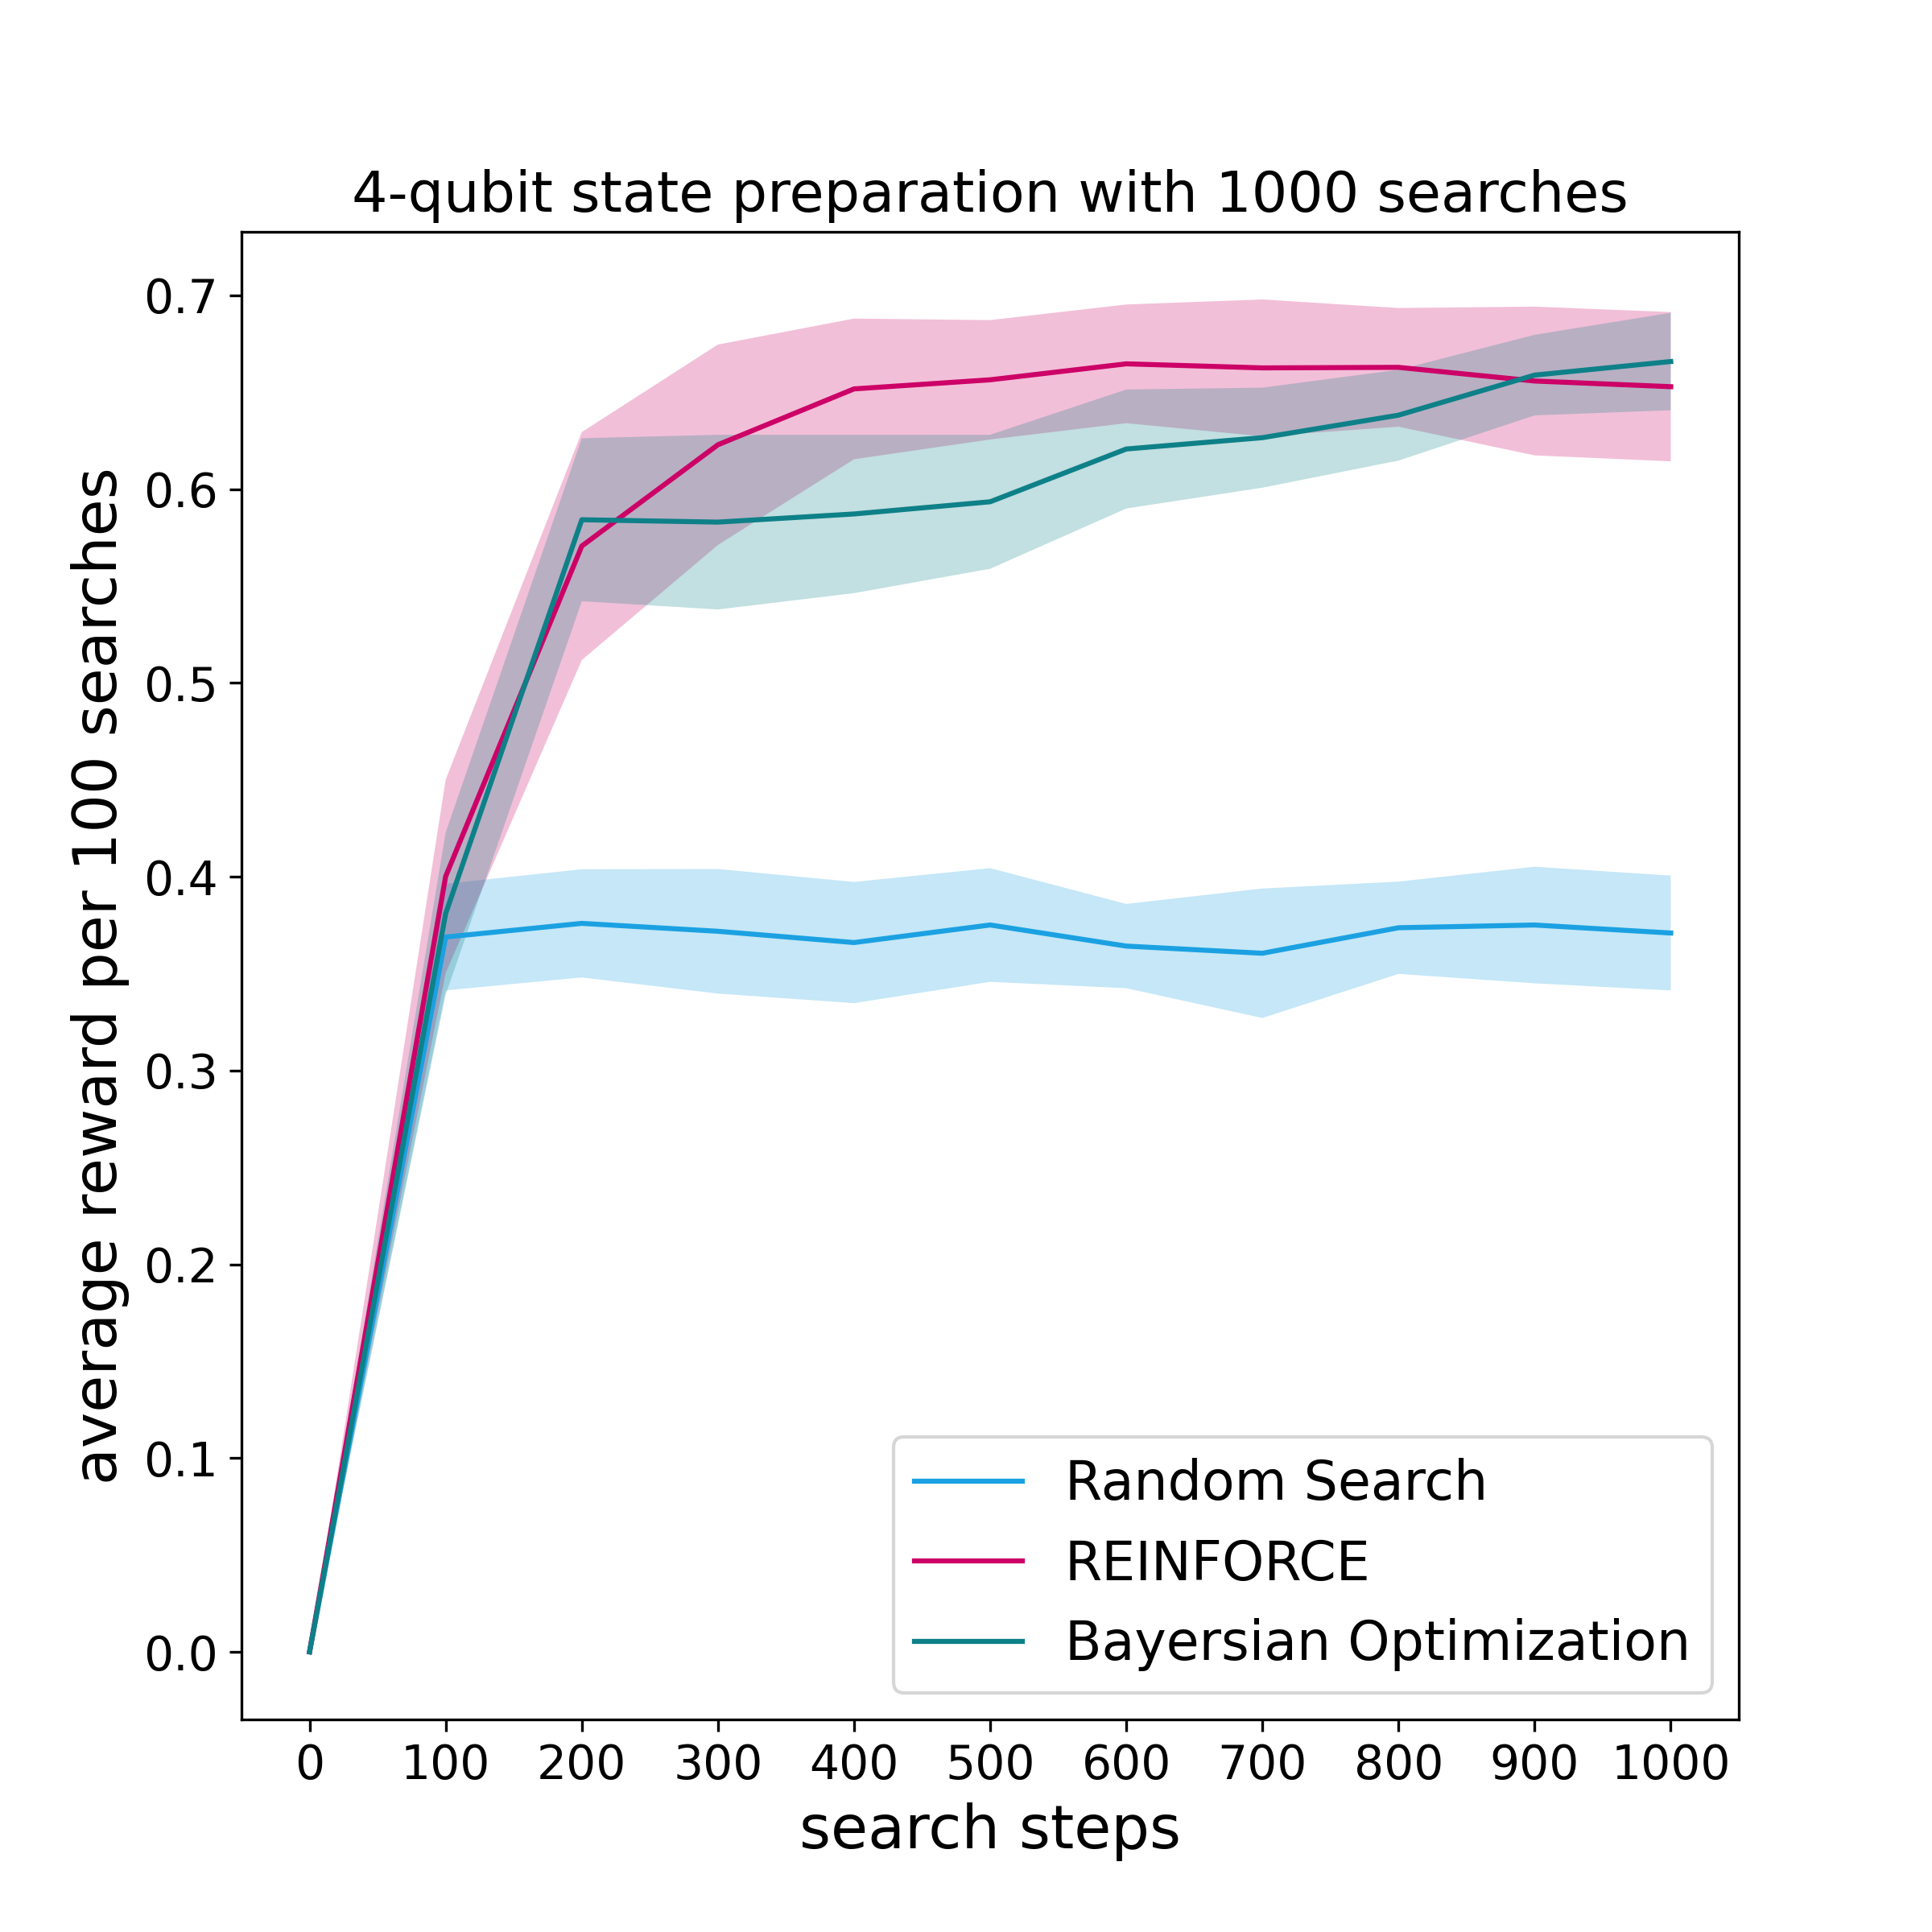
\includegraphics[width=0.49\textwidth]{images/4-qubits-fidelity_avg_reward_per_100_with_var_filling.png} %
    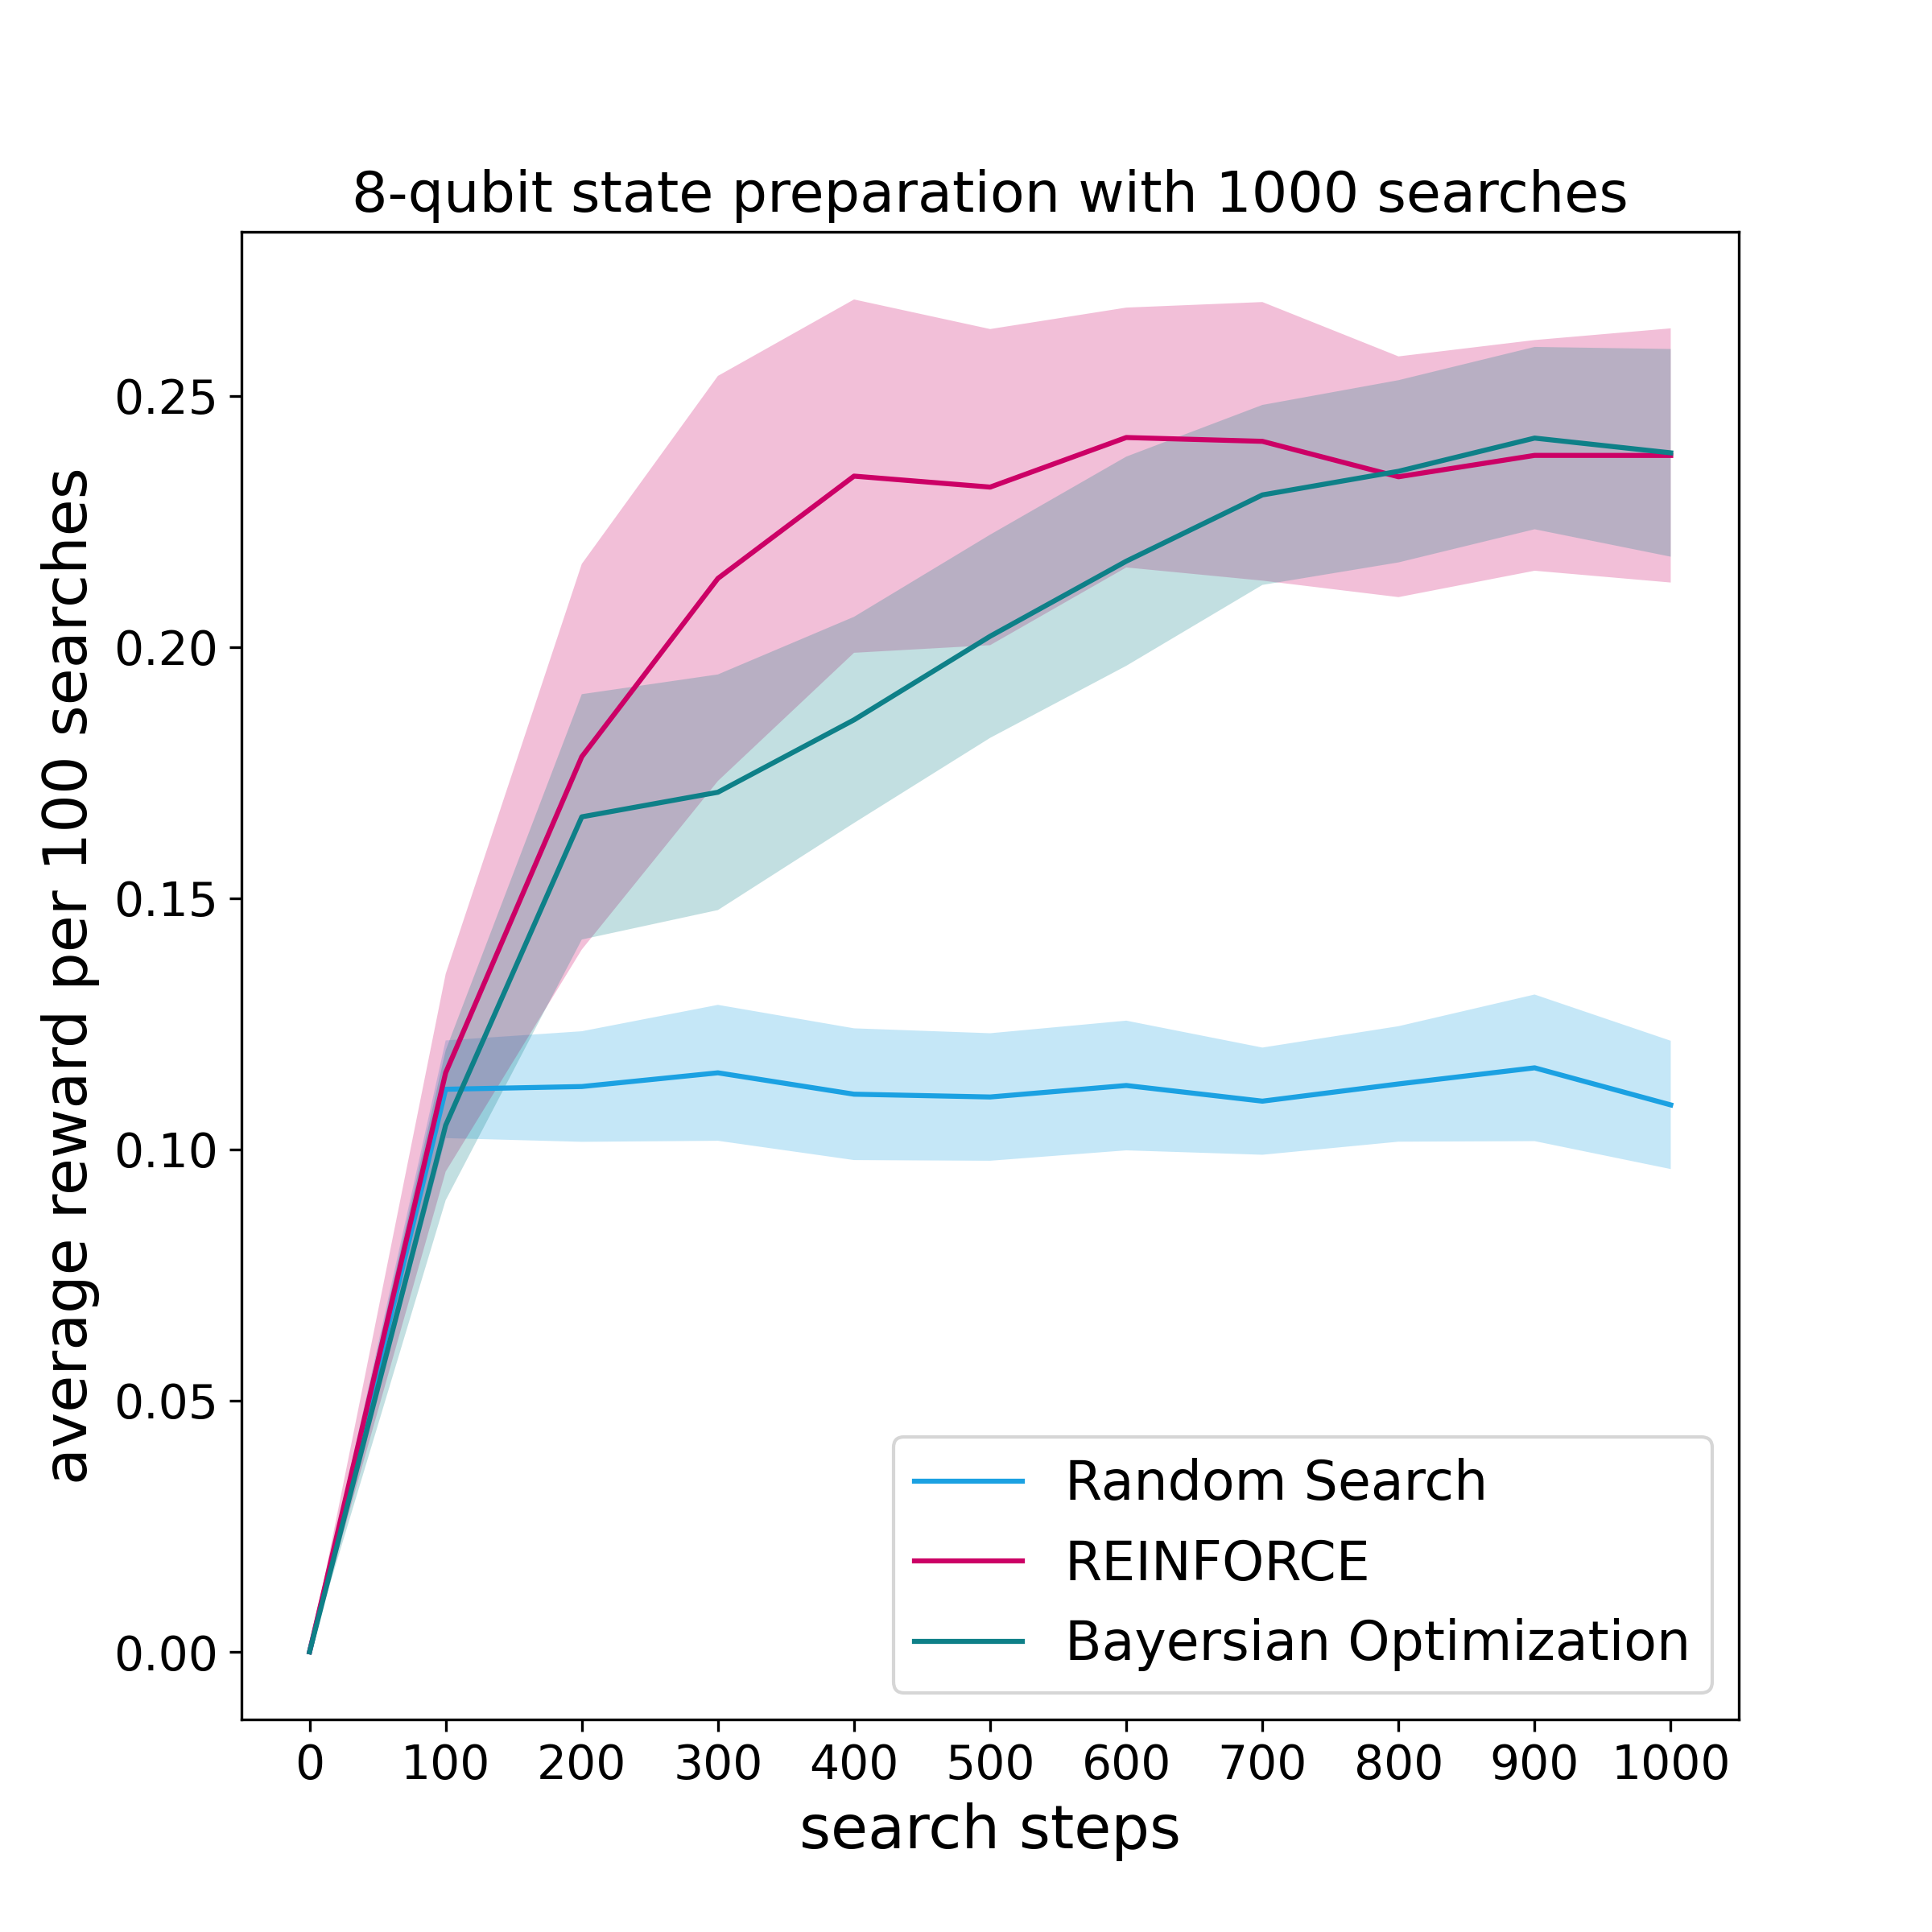
\includegraphics[width=0.49\textwidth]{images/8-qubits-fidelity_avg_reward_per_100_with_var_filling.png} %
    \caption{State preparation}
    \label{state_preparation}
    \end{subfigure}
    \hspace{0.01cm}
    \begin{subfigure}[b]{0.325\textwidth}
    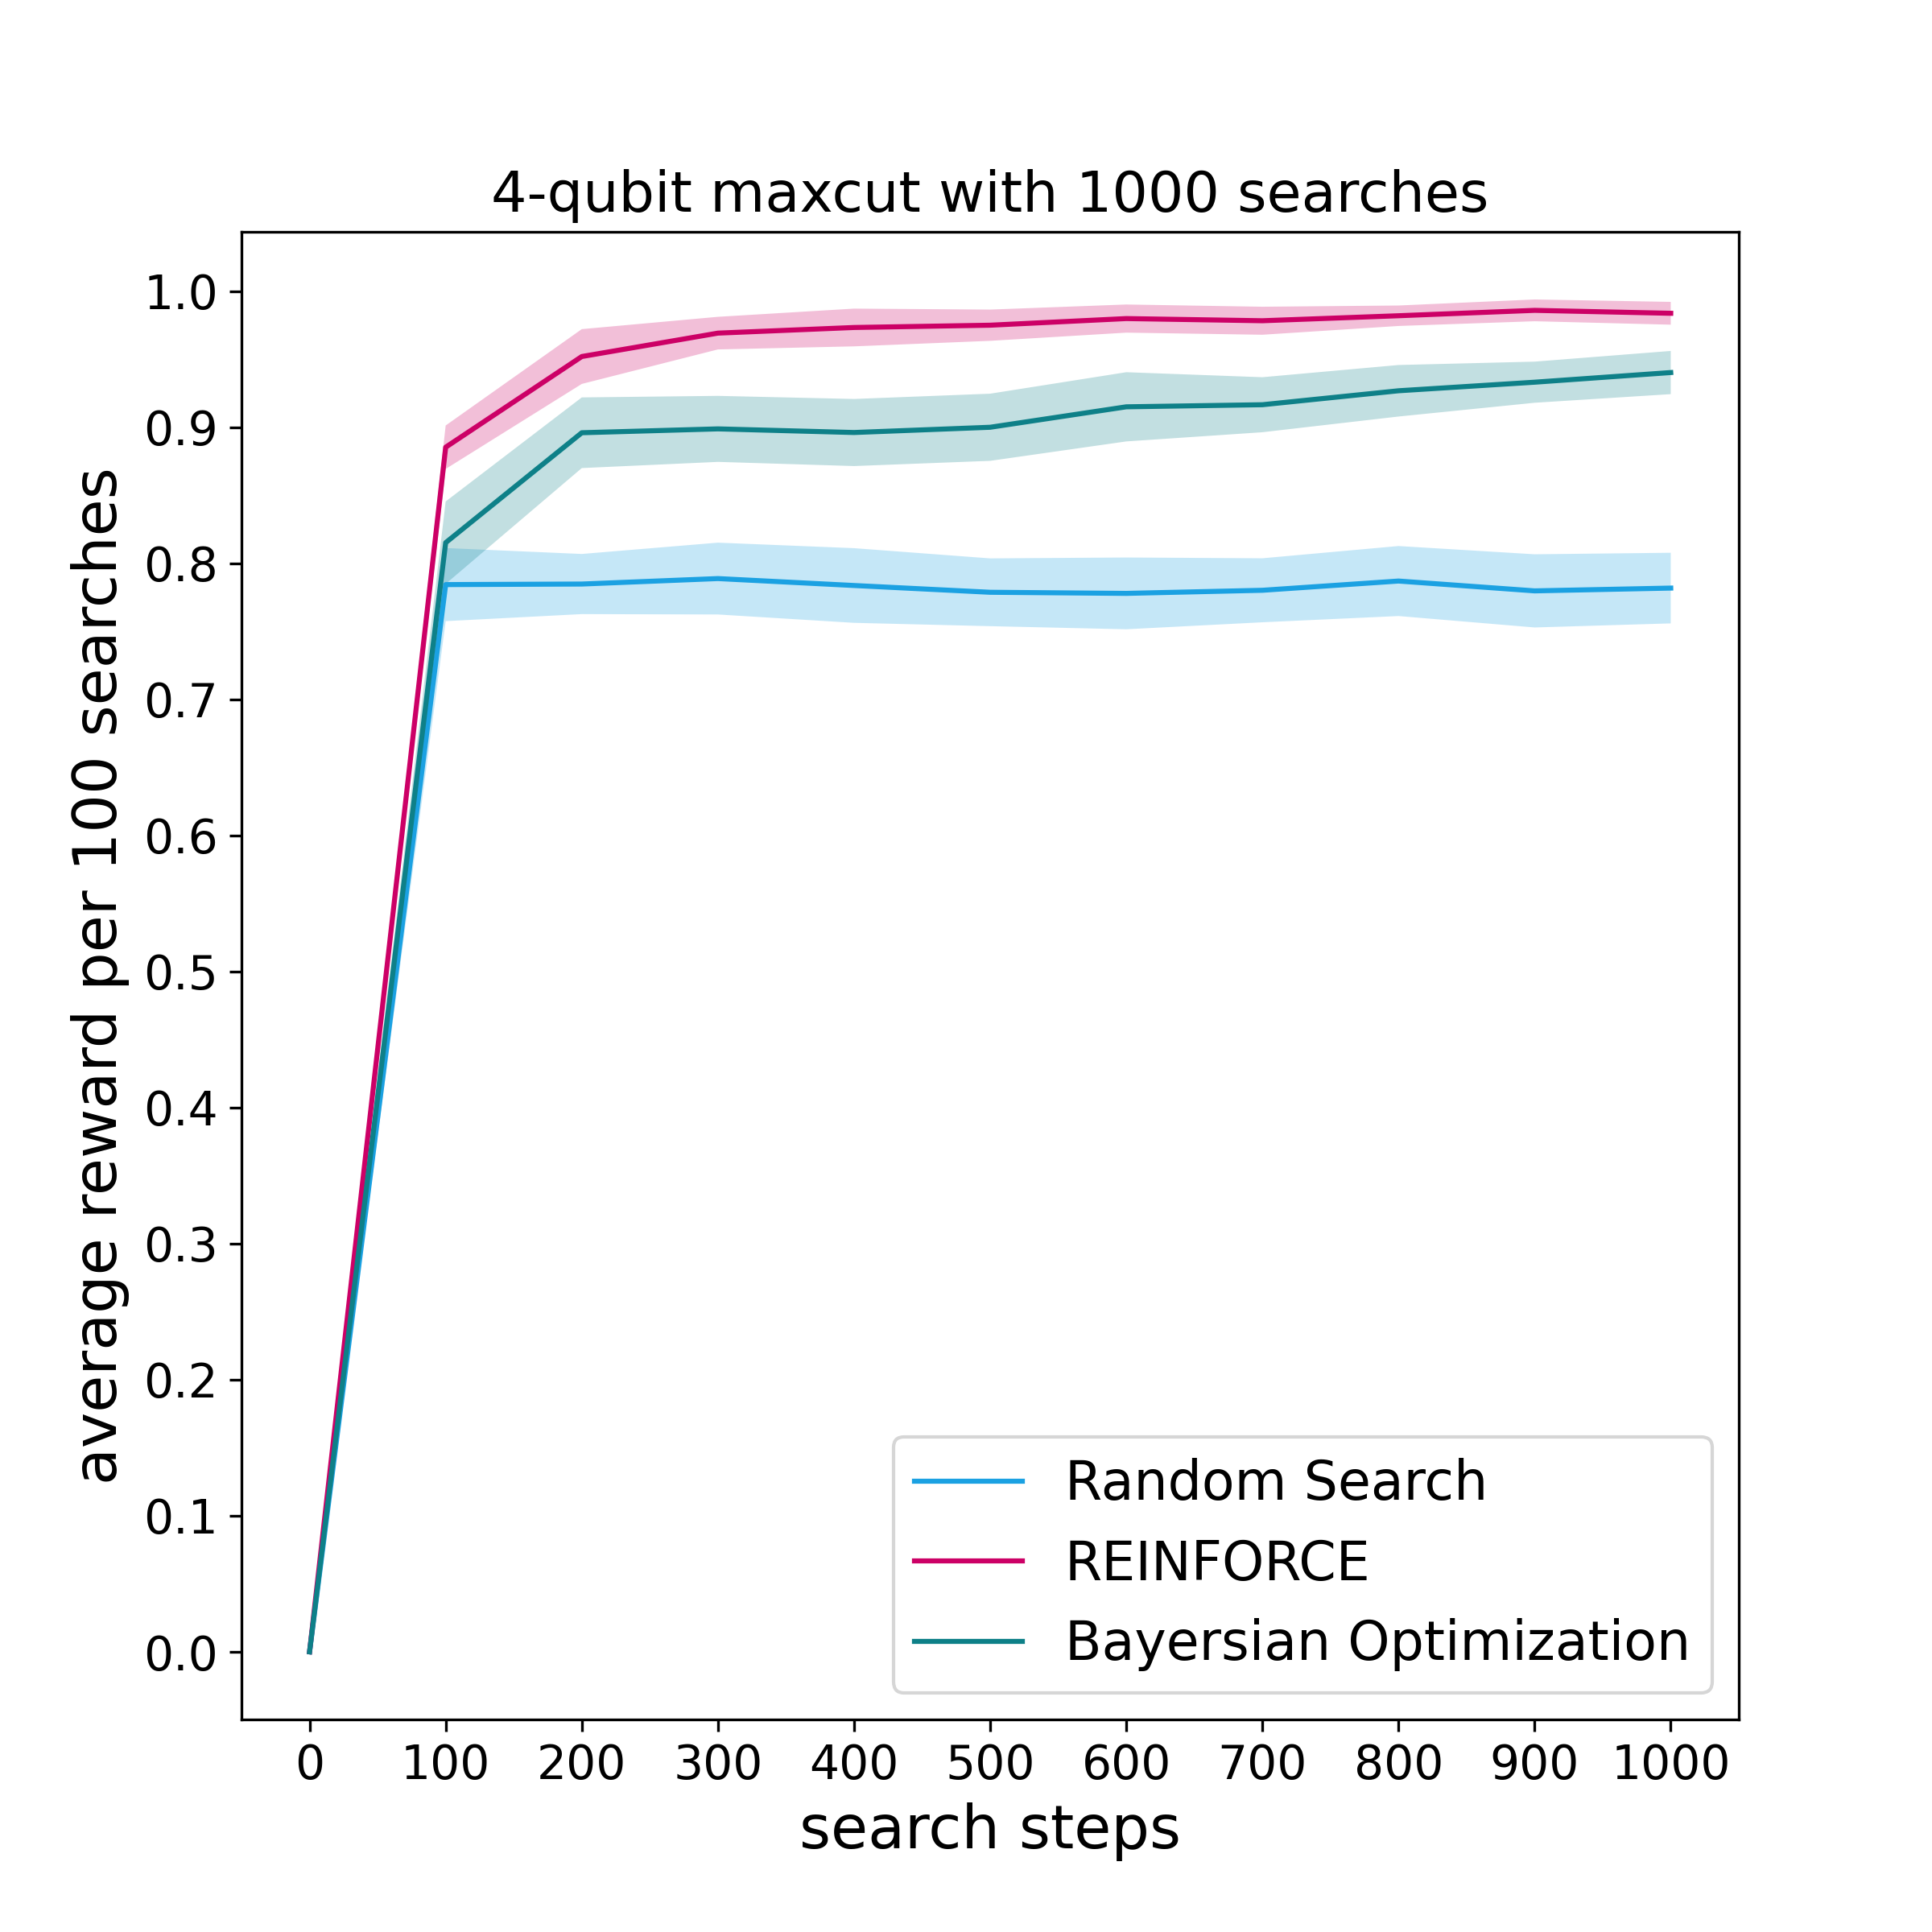
\includegraphics[width=0.49\textwidth]{images/4-qubits-maxcut_avg_reward_per_100_with_var_filling.png}
    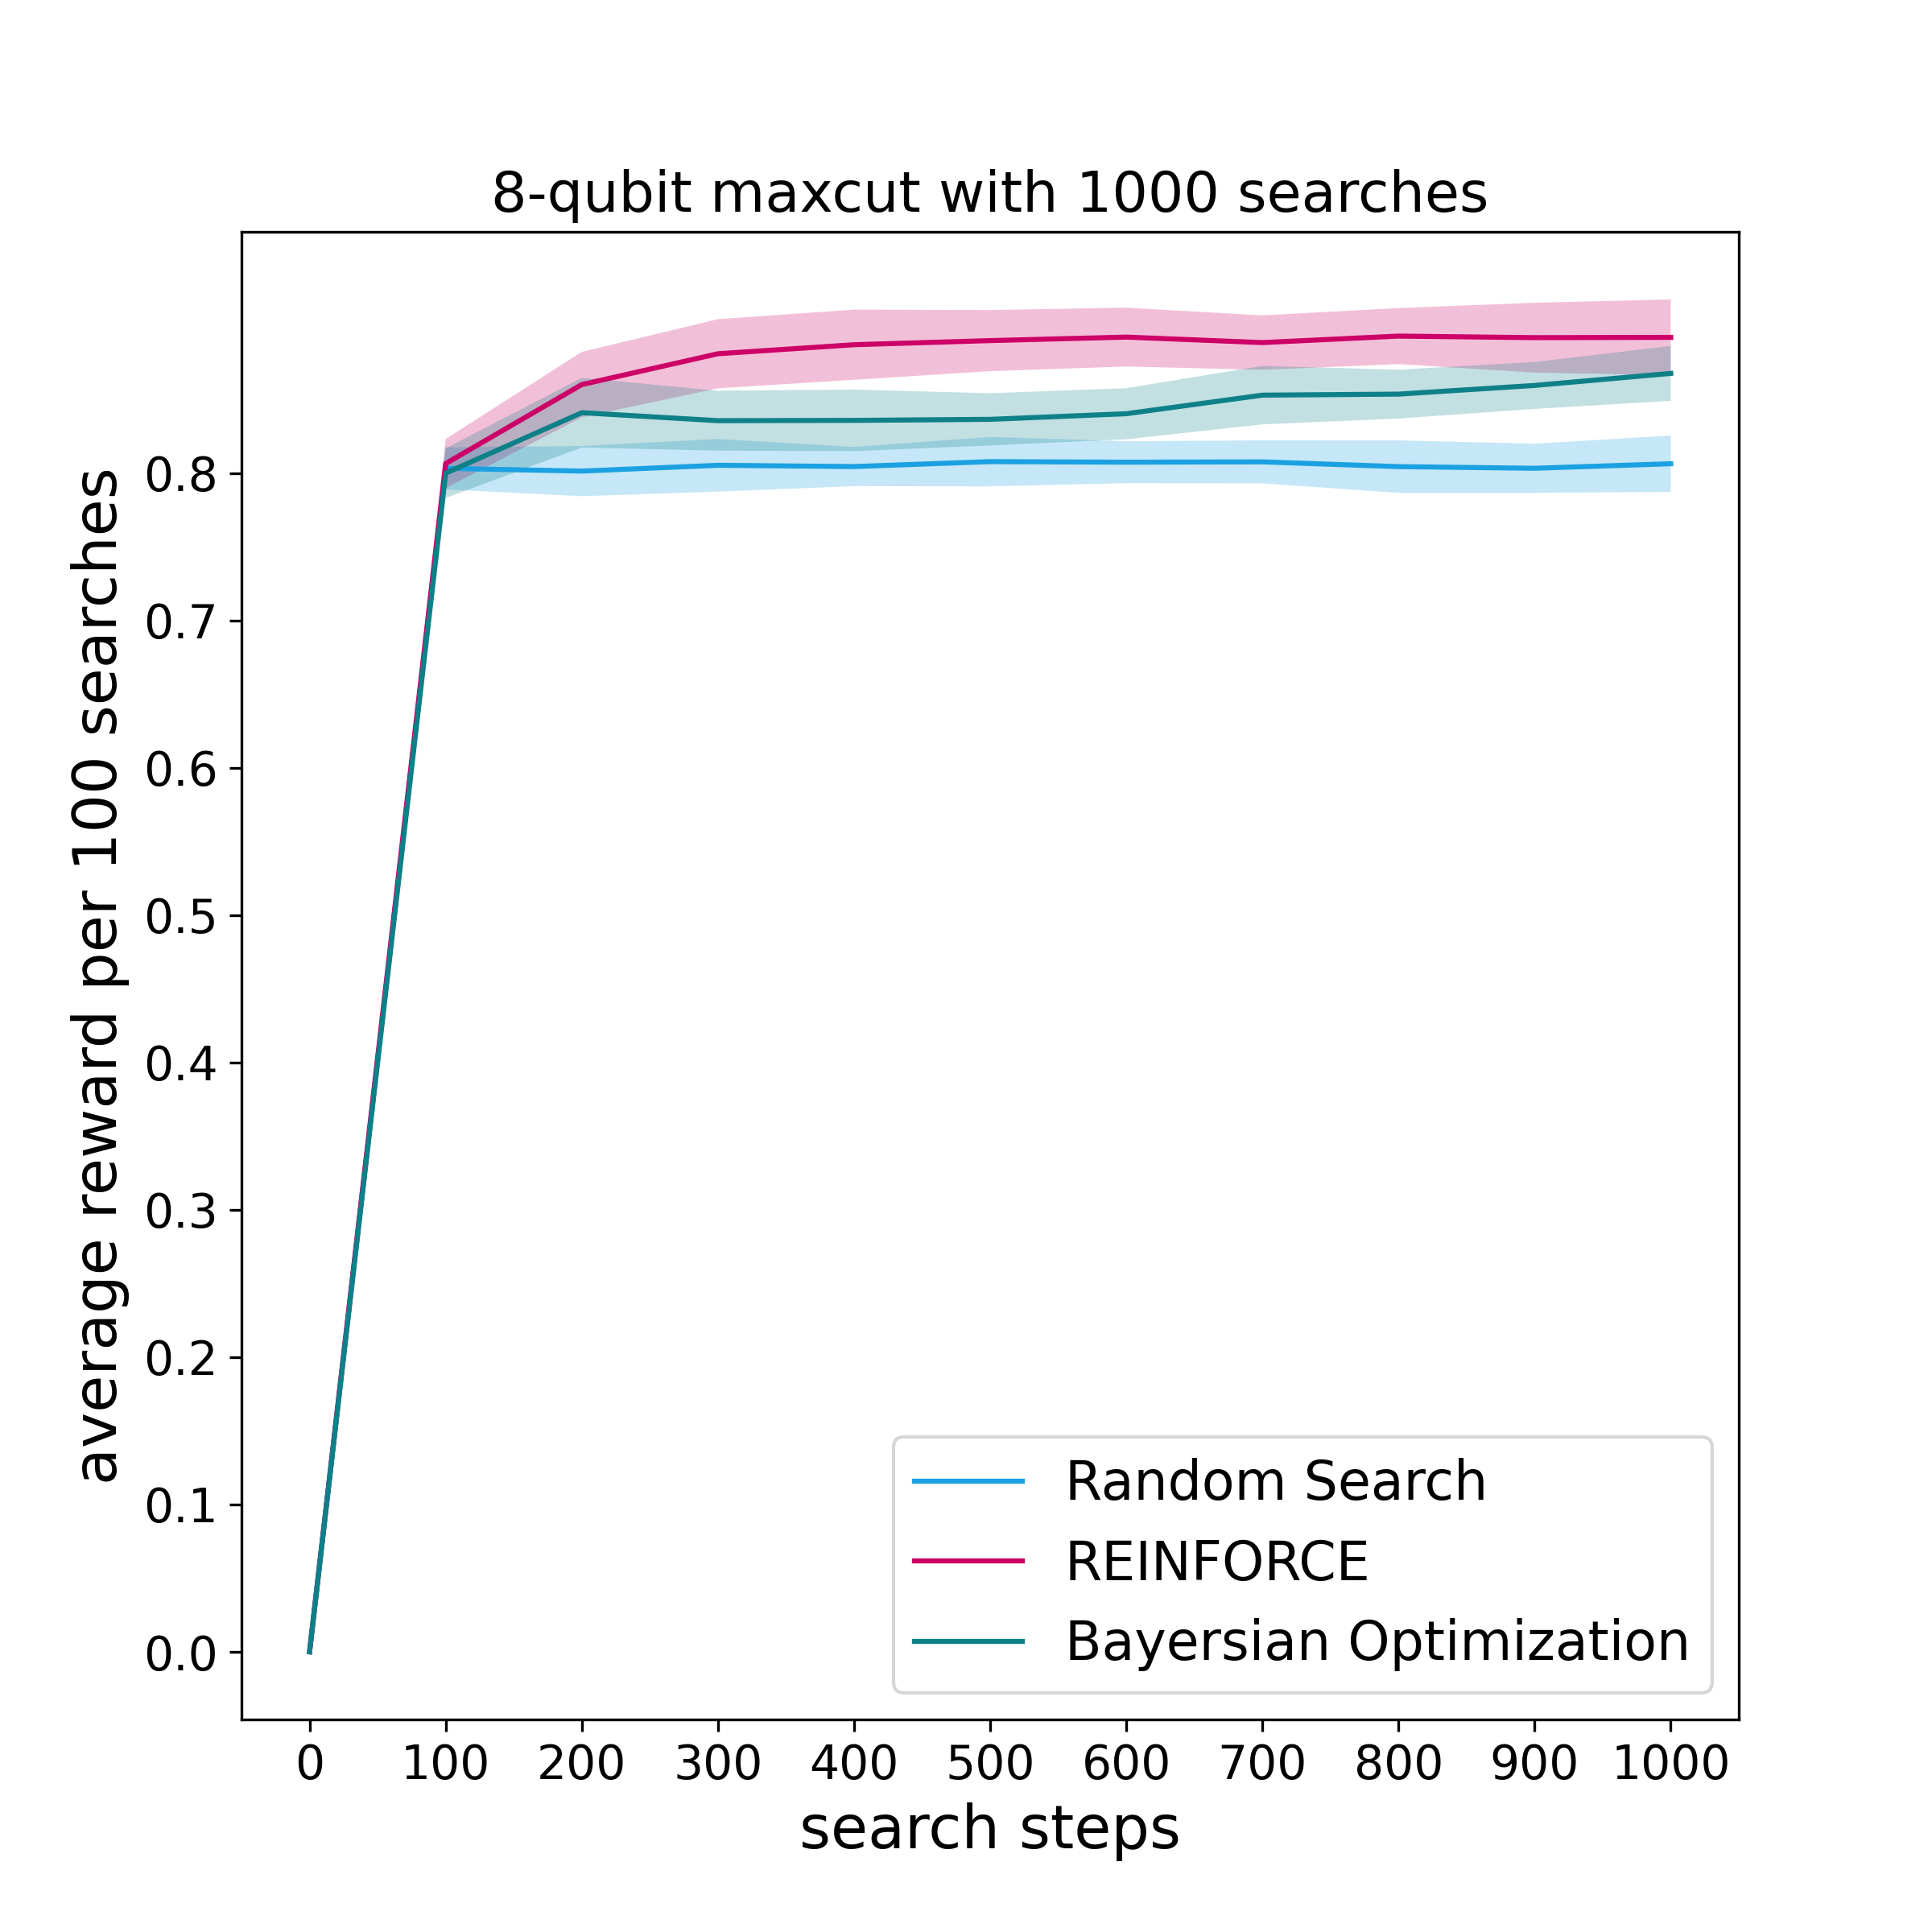
\includegraphics[width=0.49\textwidth]{images/8-qubits-maxcut_avg_reward_per_100_with_var_filling.png}
    \caption{Max-cut}
    \label{max-cut}
    \end{subfigure}
    \hspace{0.01cm}
    \begin{subfigure}[b]{0.325\textwidth}
    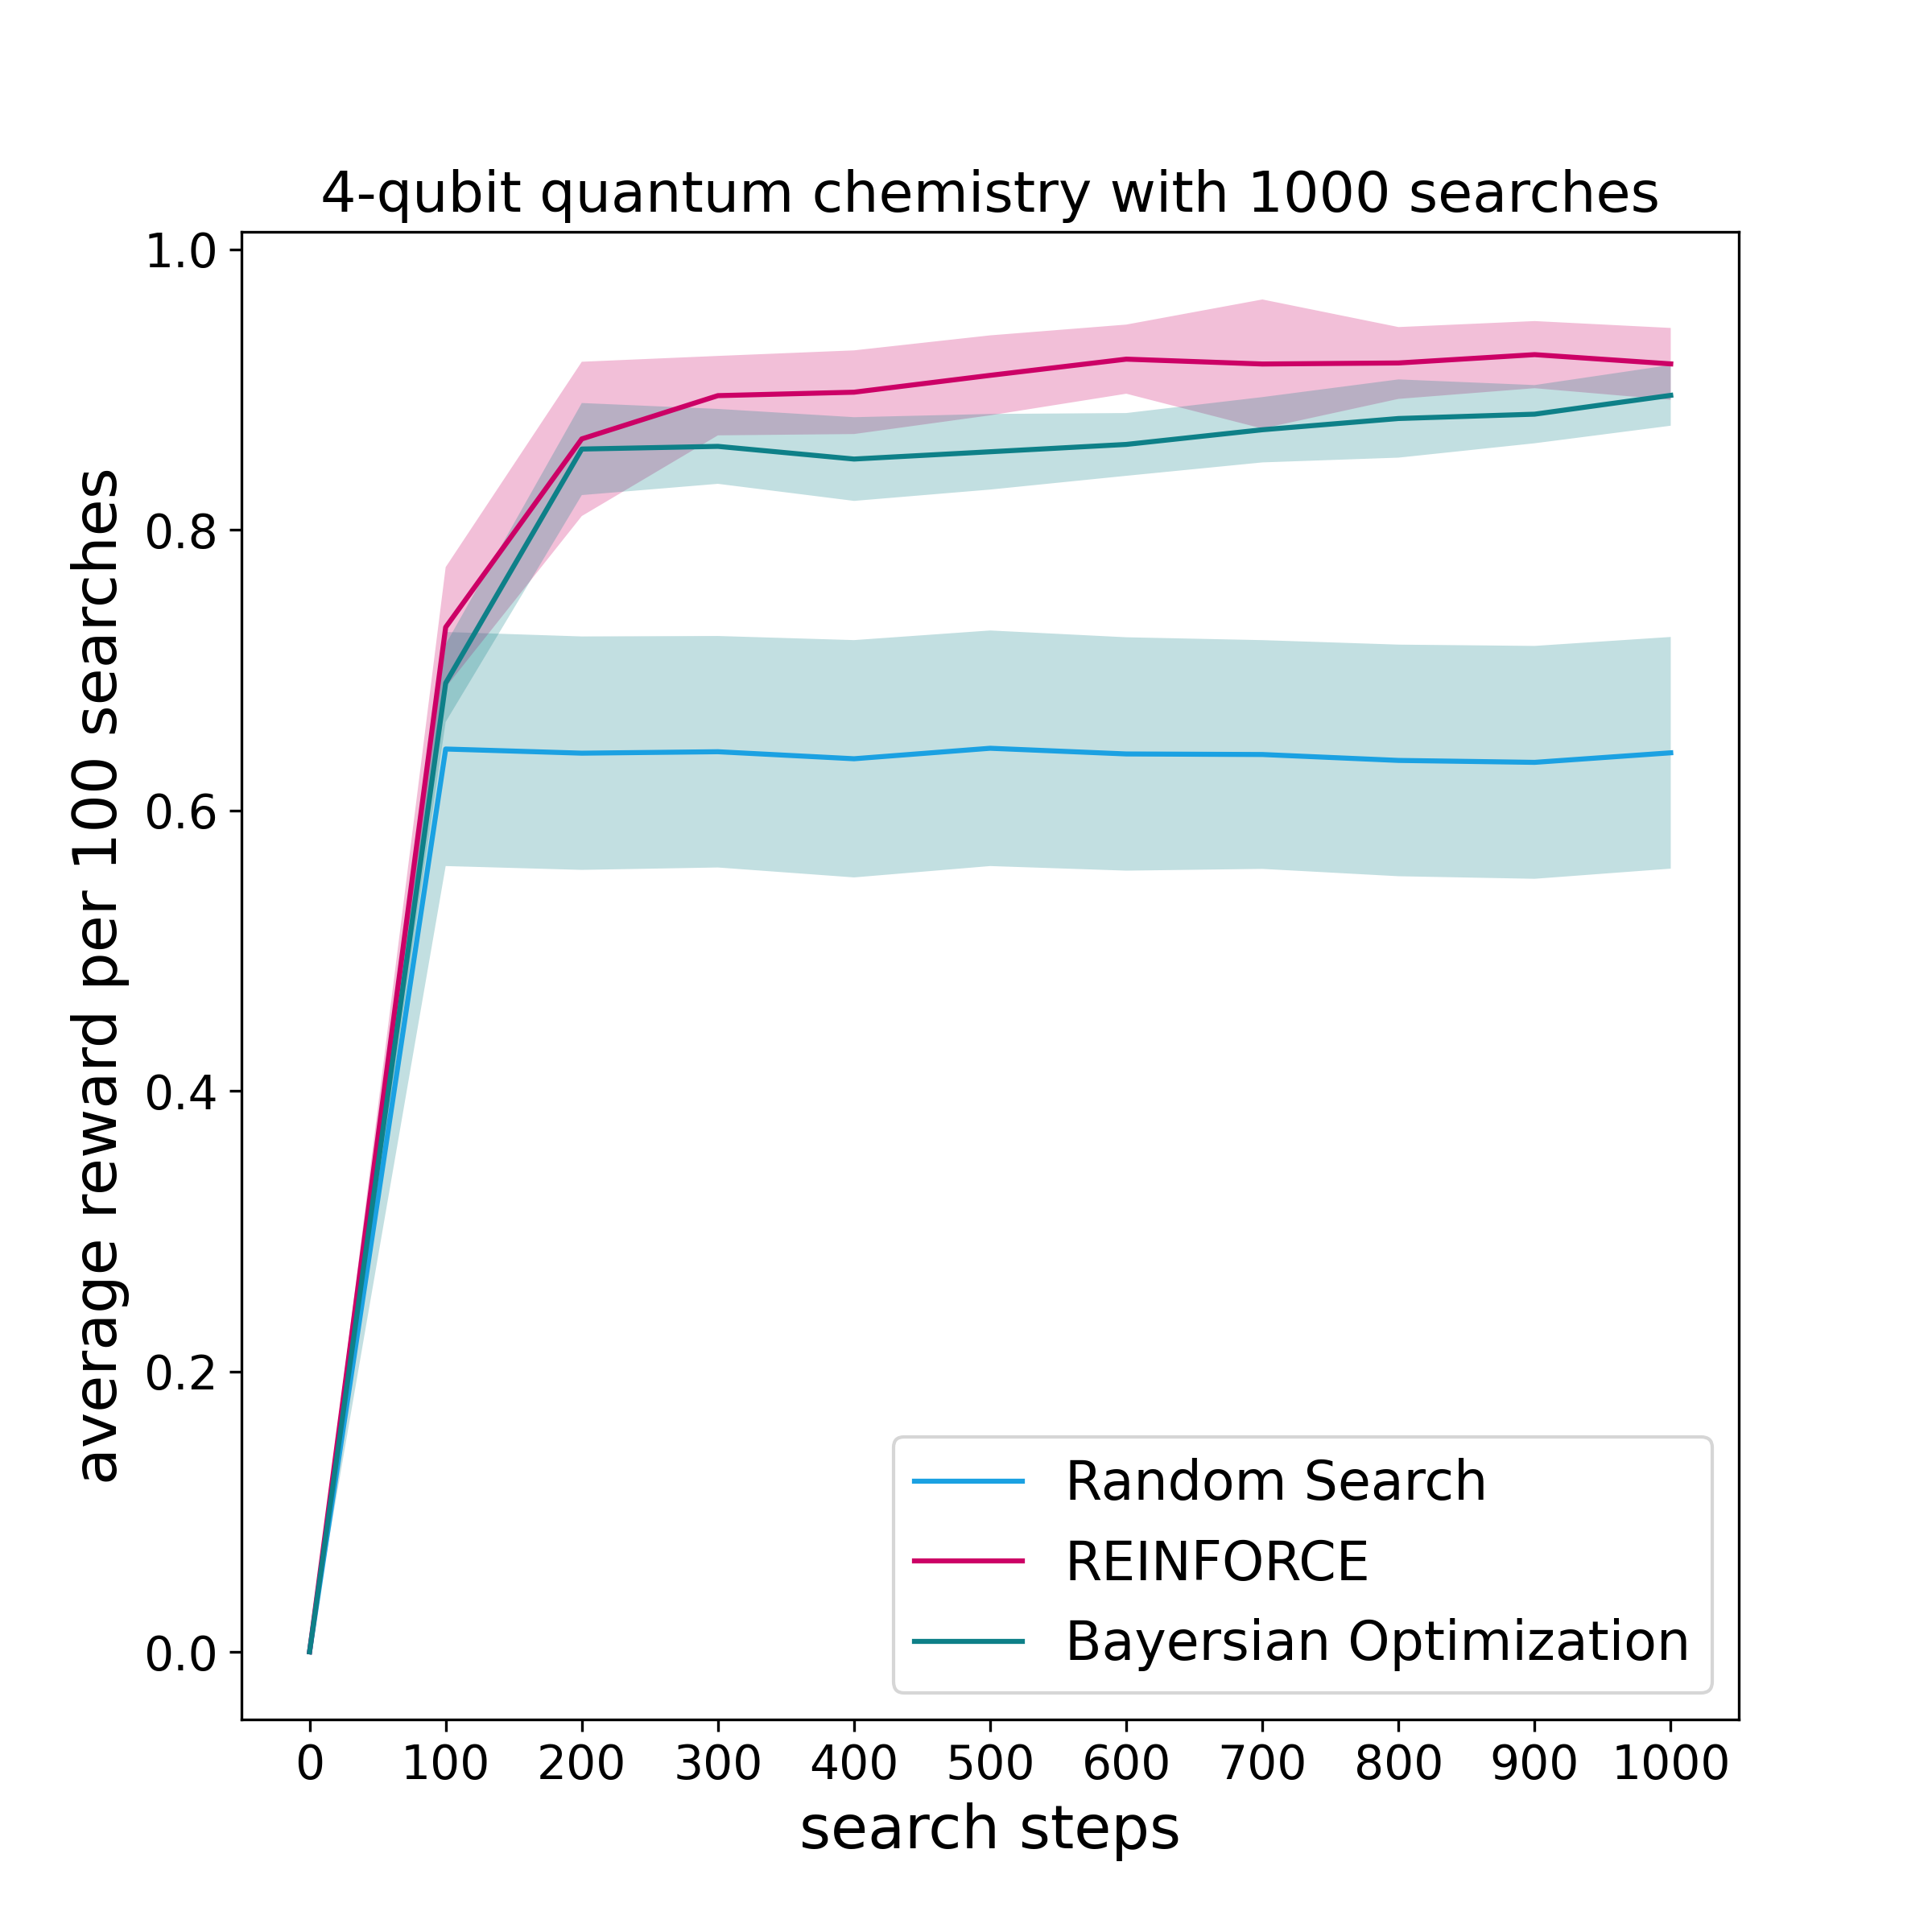
\includegraphics[width=0.49\textwidth]{images/4-qubits-vqe_avg_reward_per_100_with_var_filling.png}
    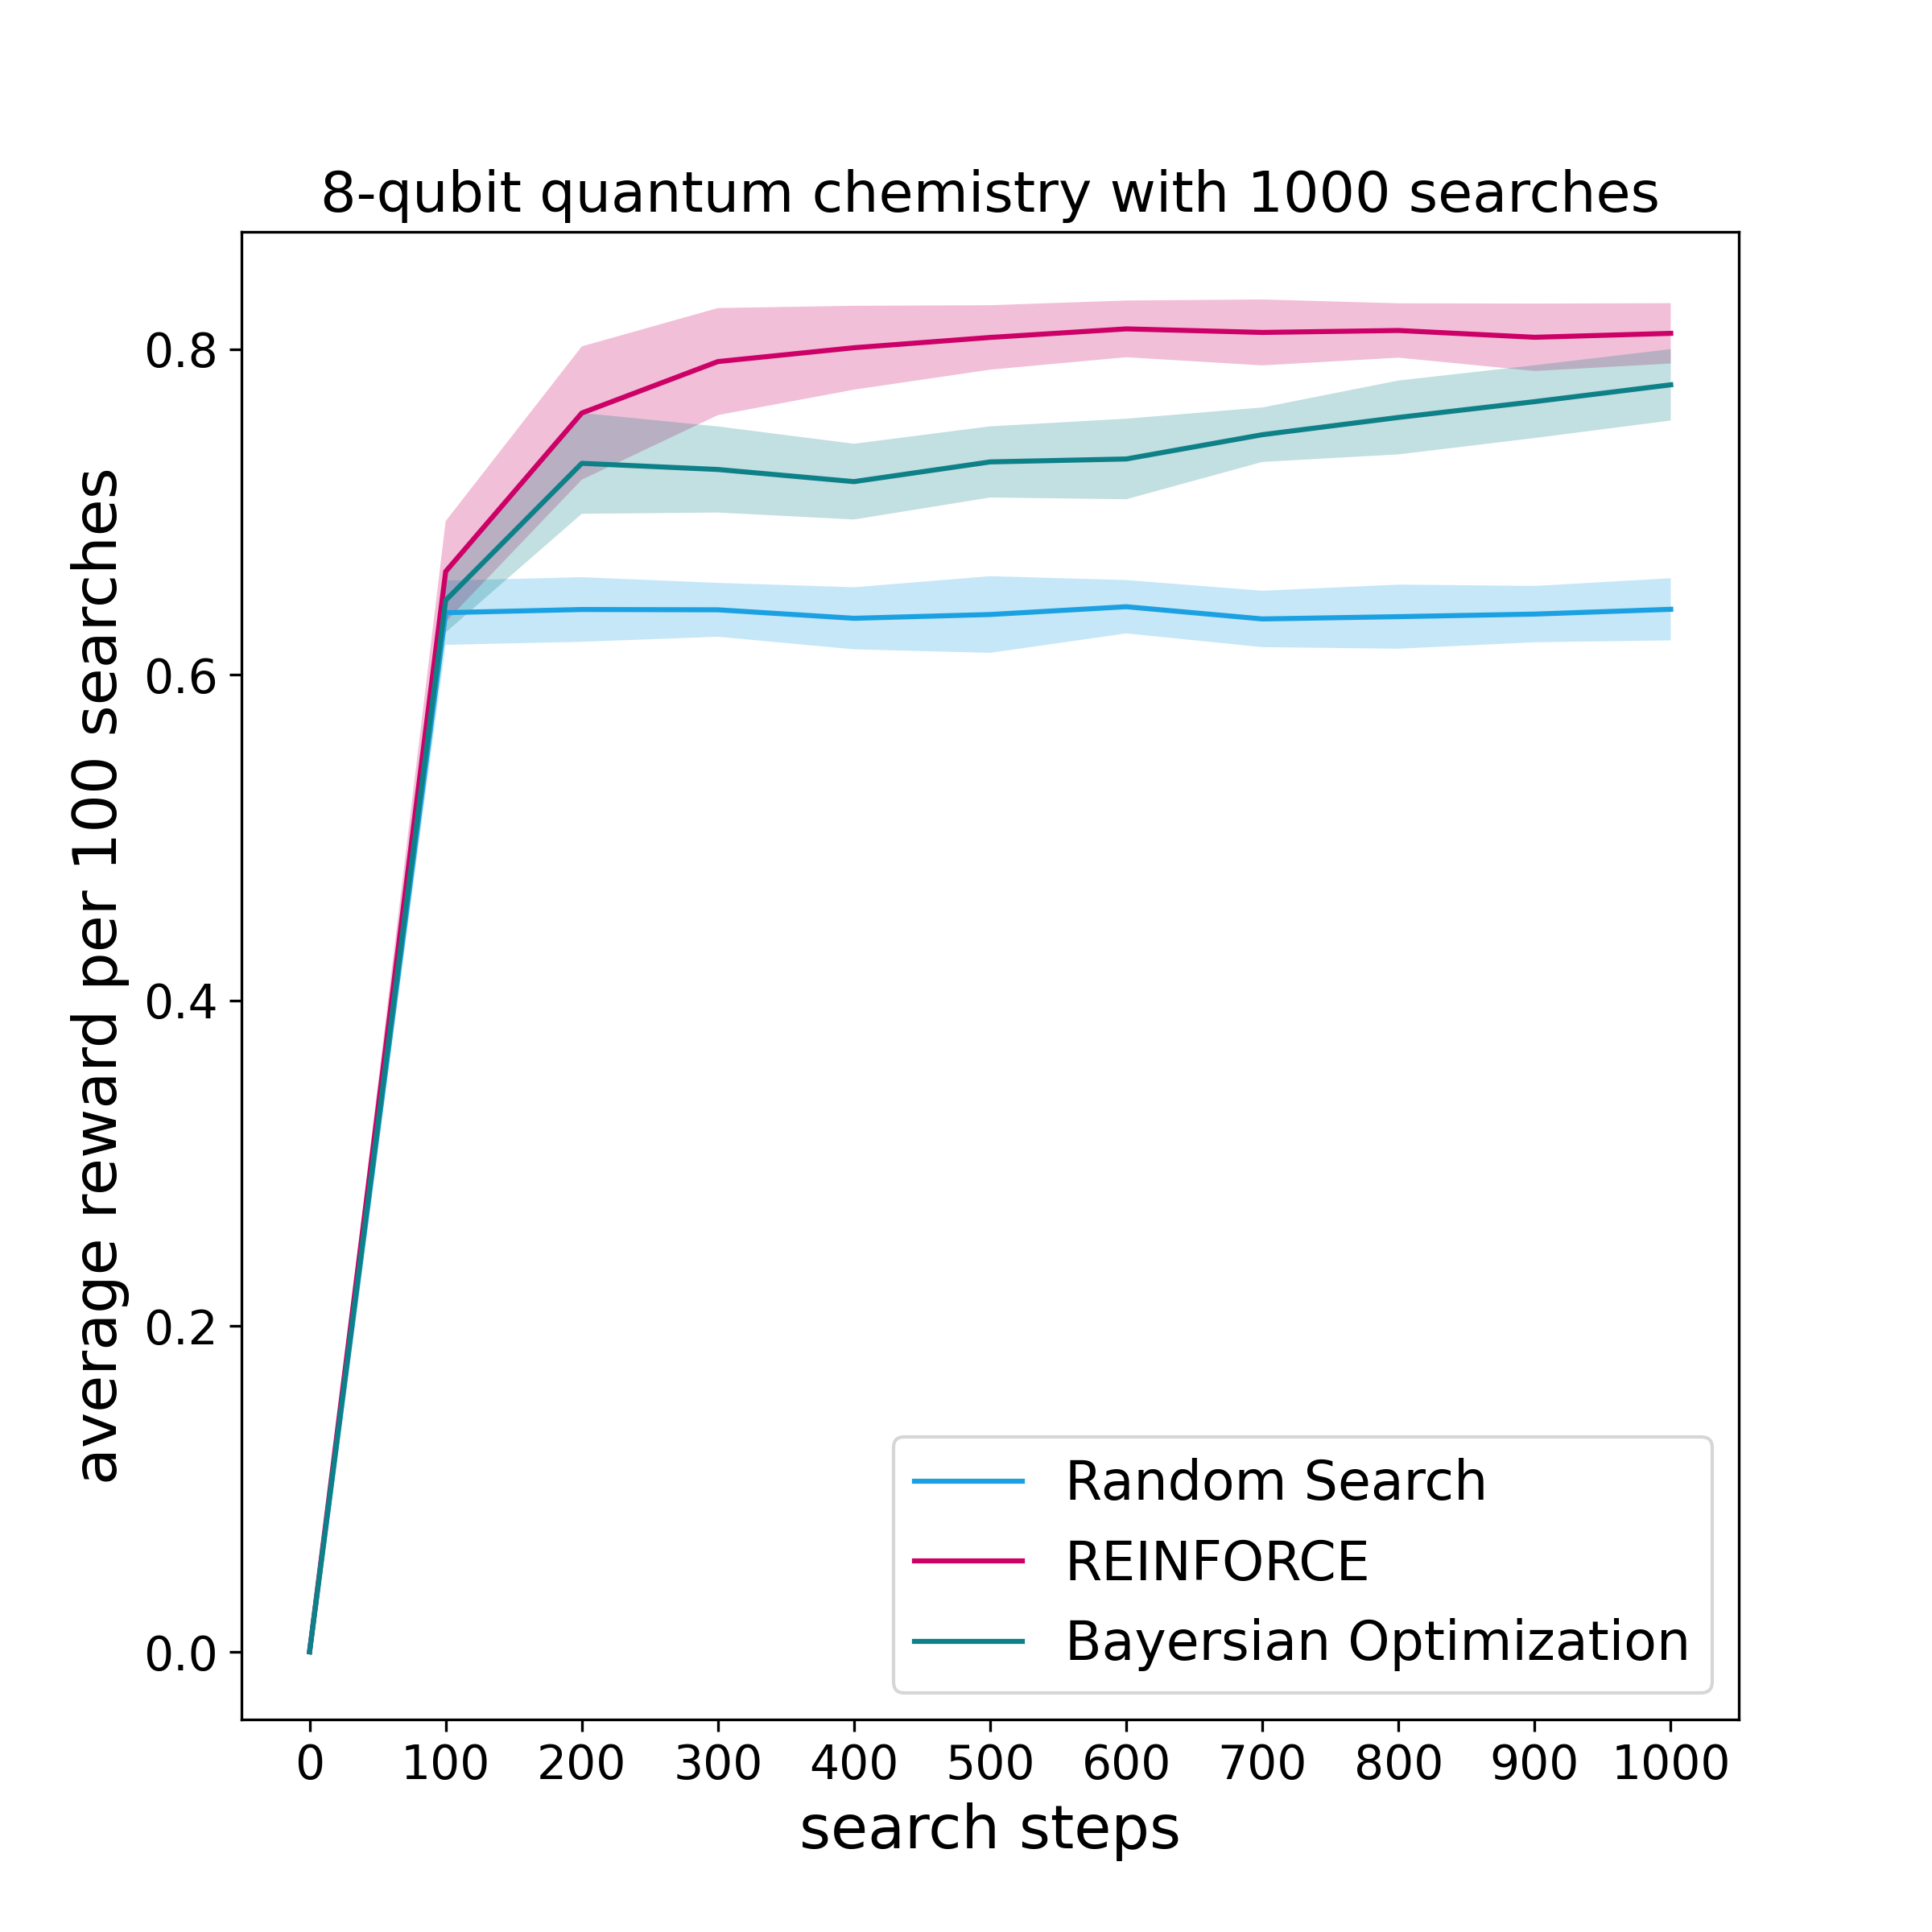
\includegraphics[width=0.49\textwidth]{images/8-qubits-vqe_avg_reward_per_100_with_var_filling.png}
    \caption{Quantum chemistry} 
    \label{quantum_chemistry}
    \end{subfigure}
    \caption{Average rewards from the six sets of experiments. In subfigures (a), (b), and (c), the left panels show results from the 4-qubit experiments, while the right panels show results from the 8-qubit experiments. Each plot presents the average reward across 50 independent runs (each with different random seeds) given 1000 search queries. The shaded areas in the plots represent the standard deviation of the average rewards.}
    \label{average_reward}
\end{center}
\end{figure}

\begin{comment}
\begin{figure}[ht]
\begin{center}
    \begin{subfigure}[b]{0.49\textwidth}
    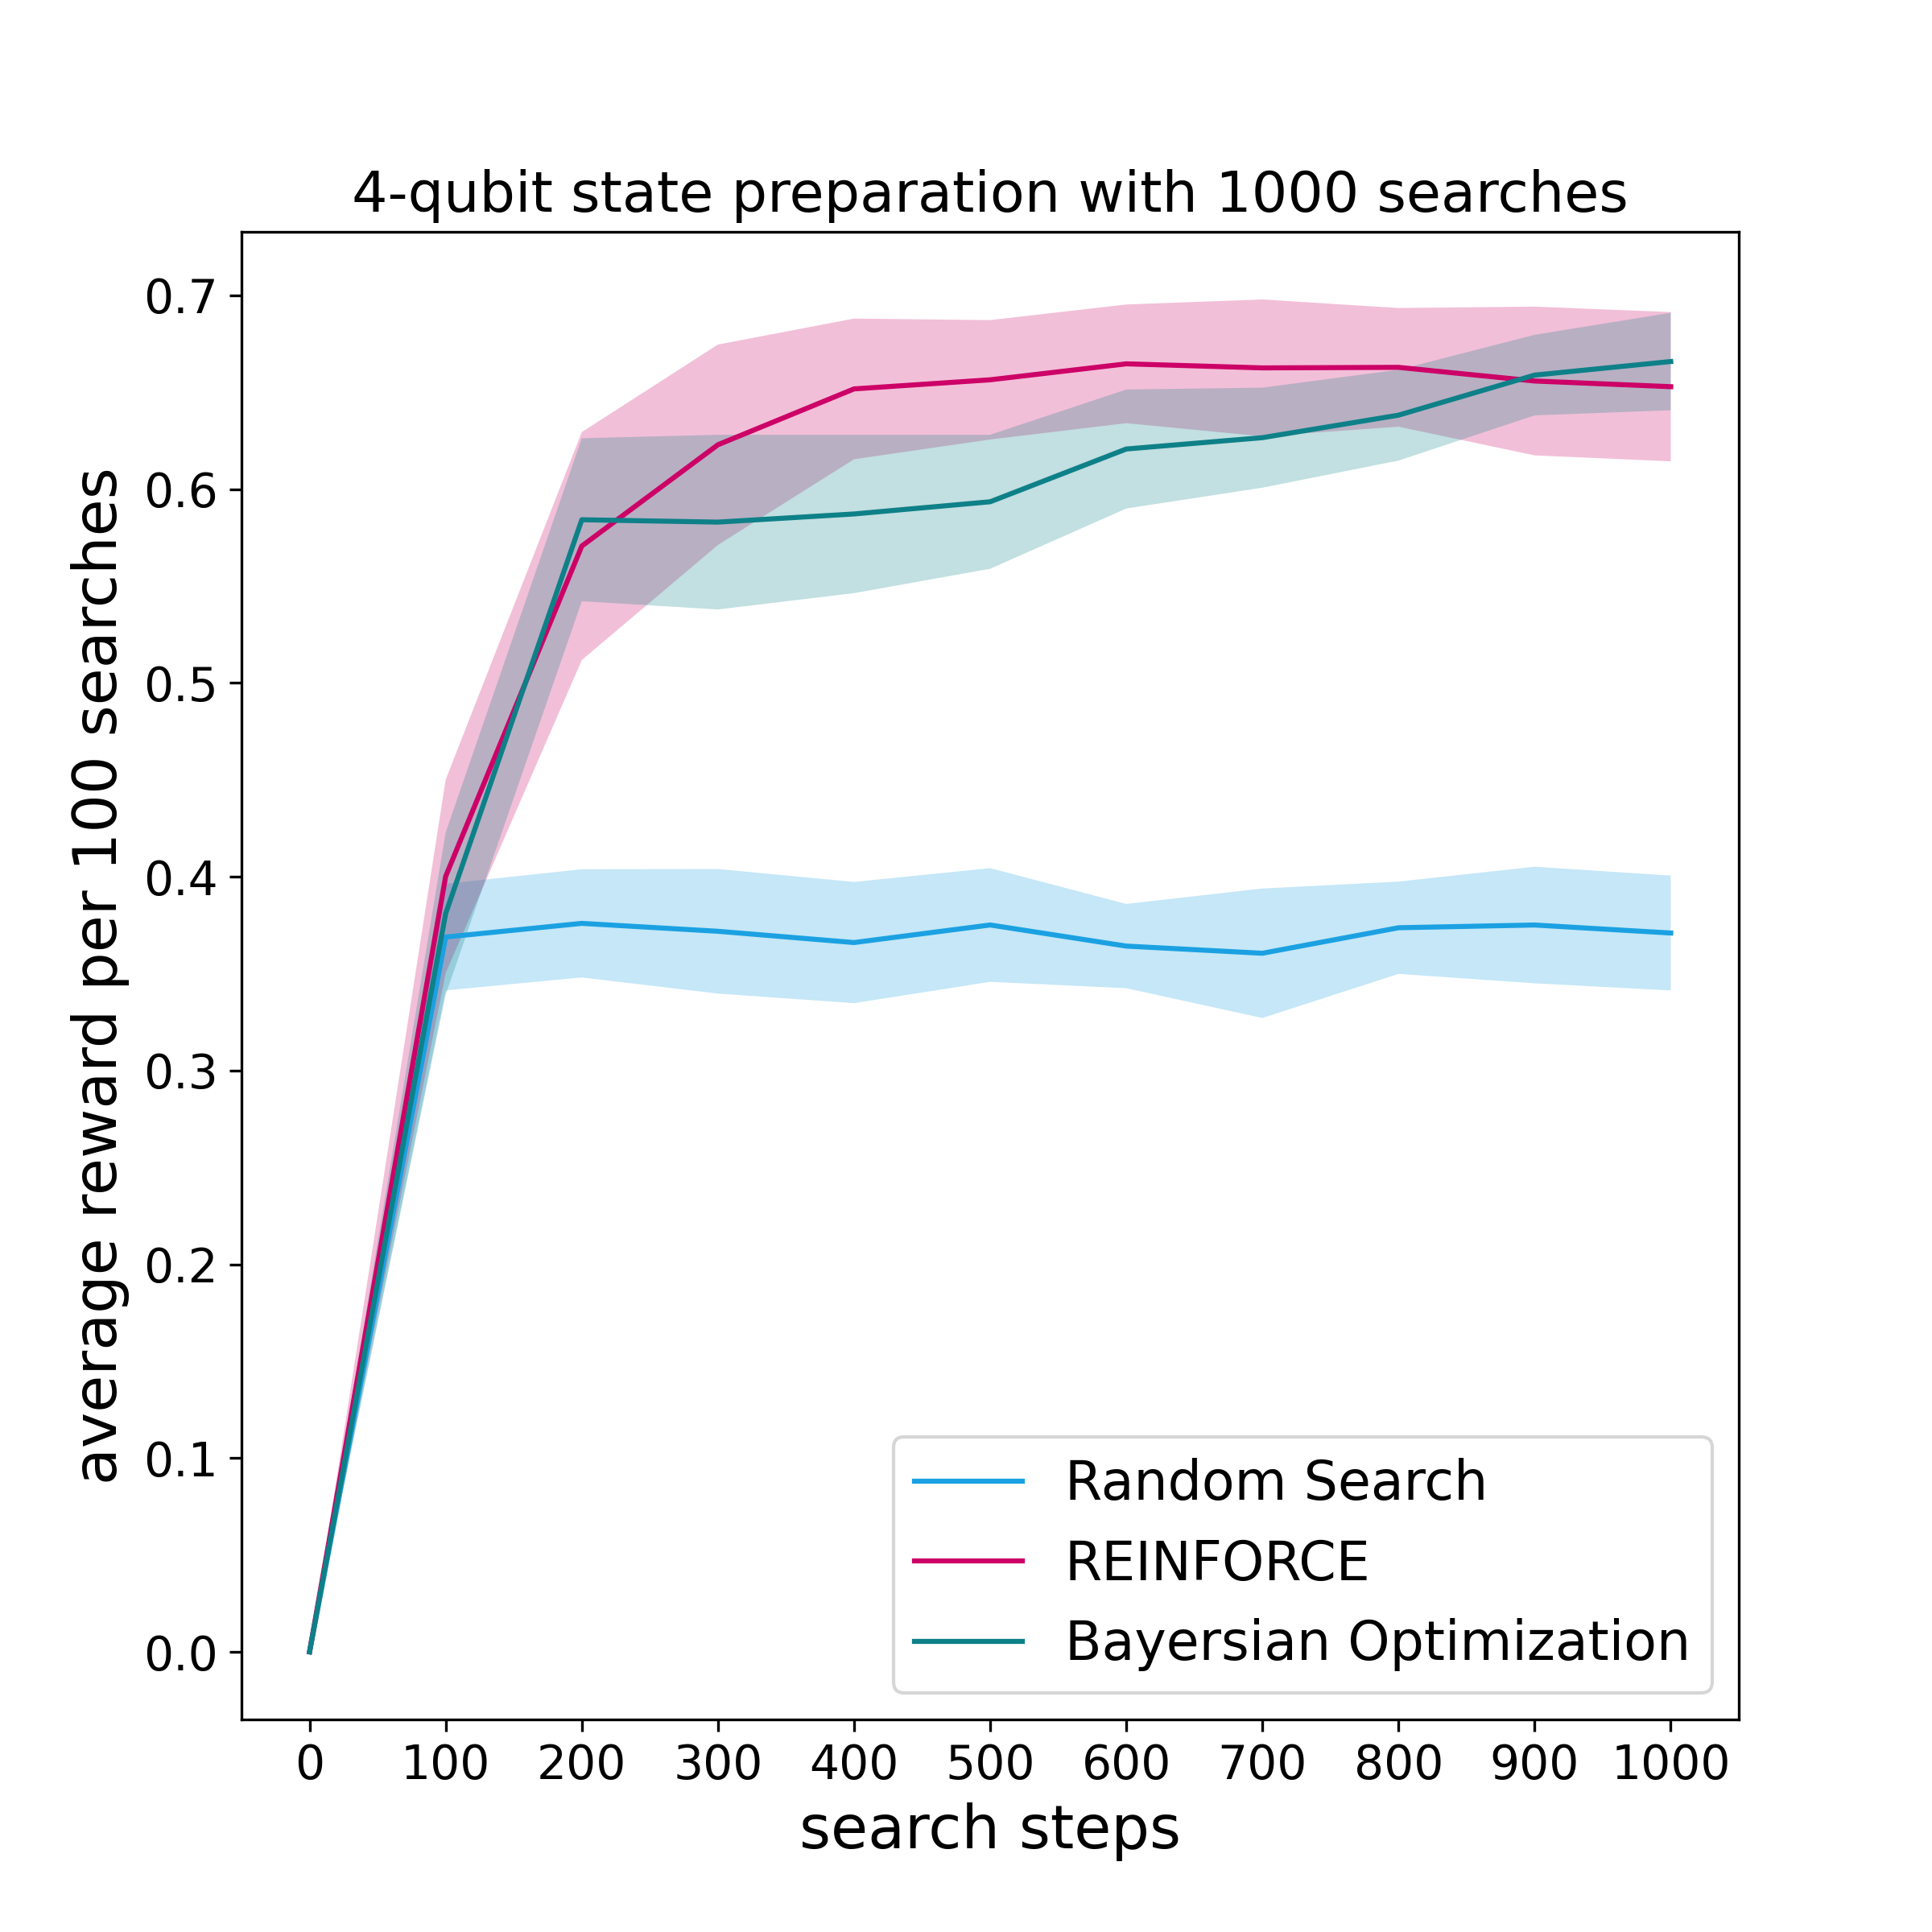
\includegraphics[width=0.49\textwidth]{images/4-qubits-fidelity_avg_reward_per_100_with_var_filling.png} %
    \includegraphics[width=0.49\textwidth]{images/4-qubits-fidelity_regret_fidelity_from_200_with_var_willing.png} %
    \label{4-qubit_fidelity_regret}
    \caption{4-qubit state preparation}
    \label{4-qubit_fidelity}
    \end{subfigure}
    \hfill
    \begin{subfigure}[b]{0.49\textwidth}
    \centering
    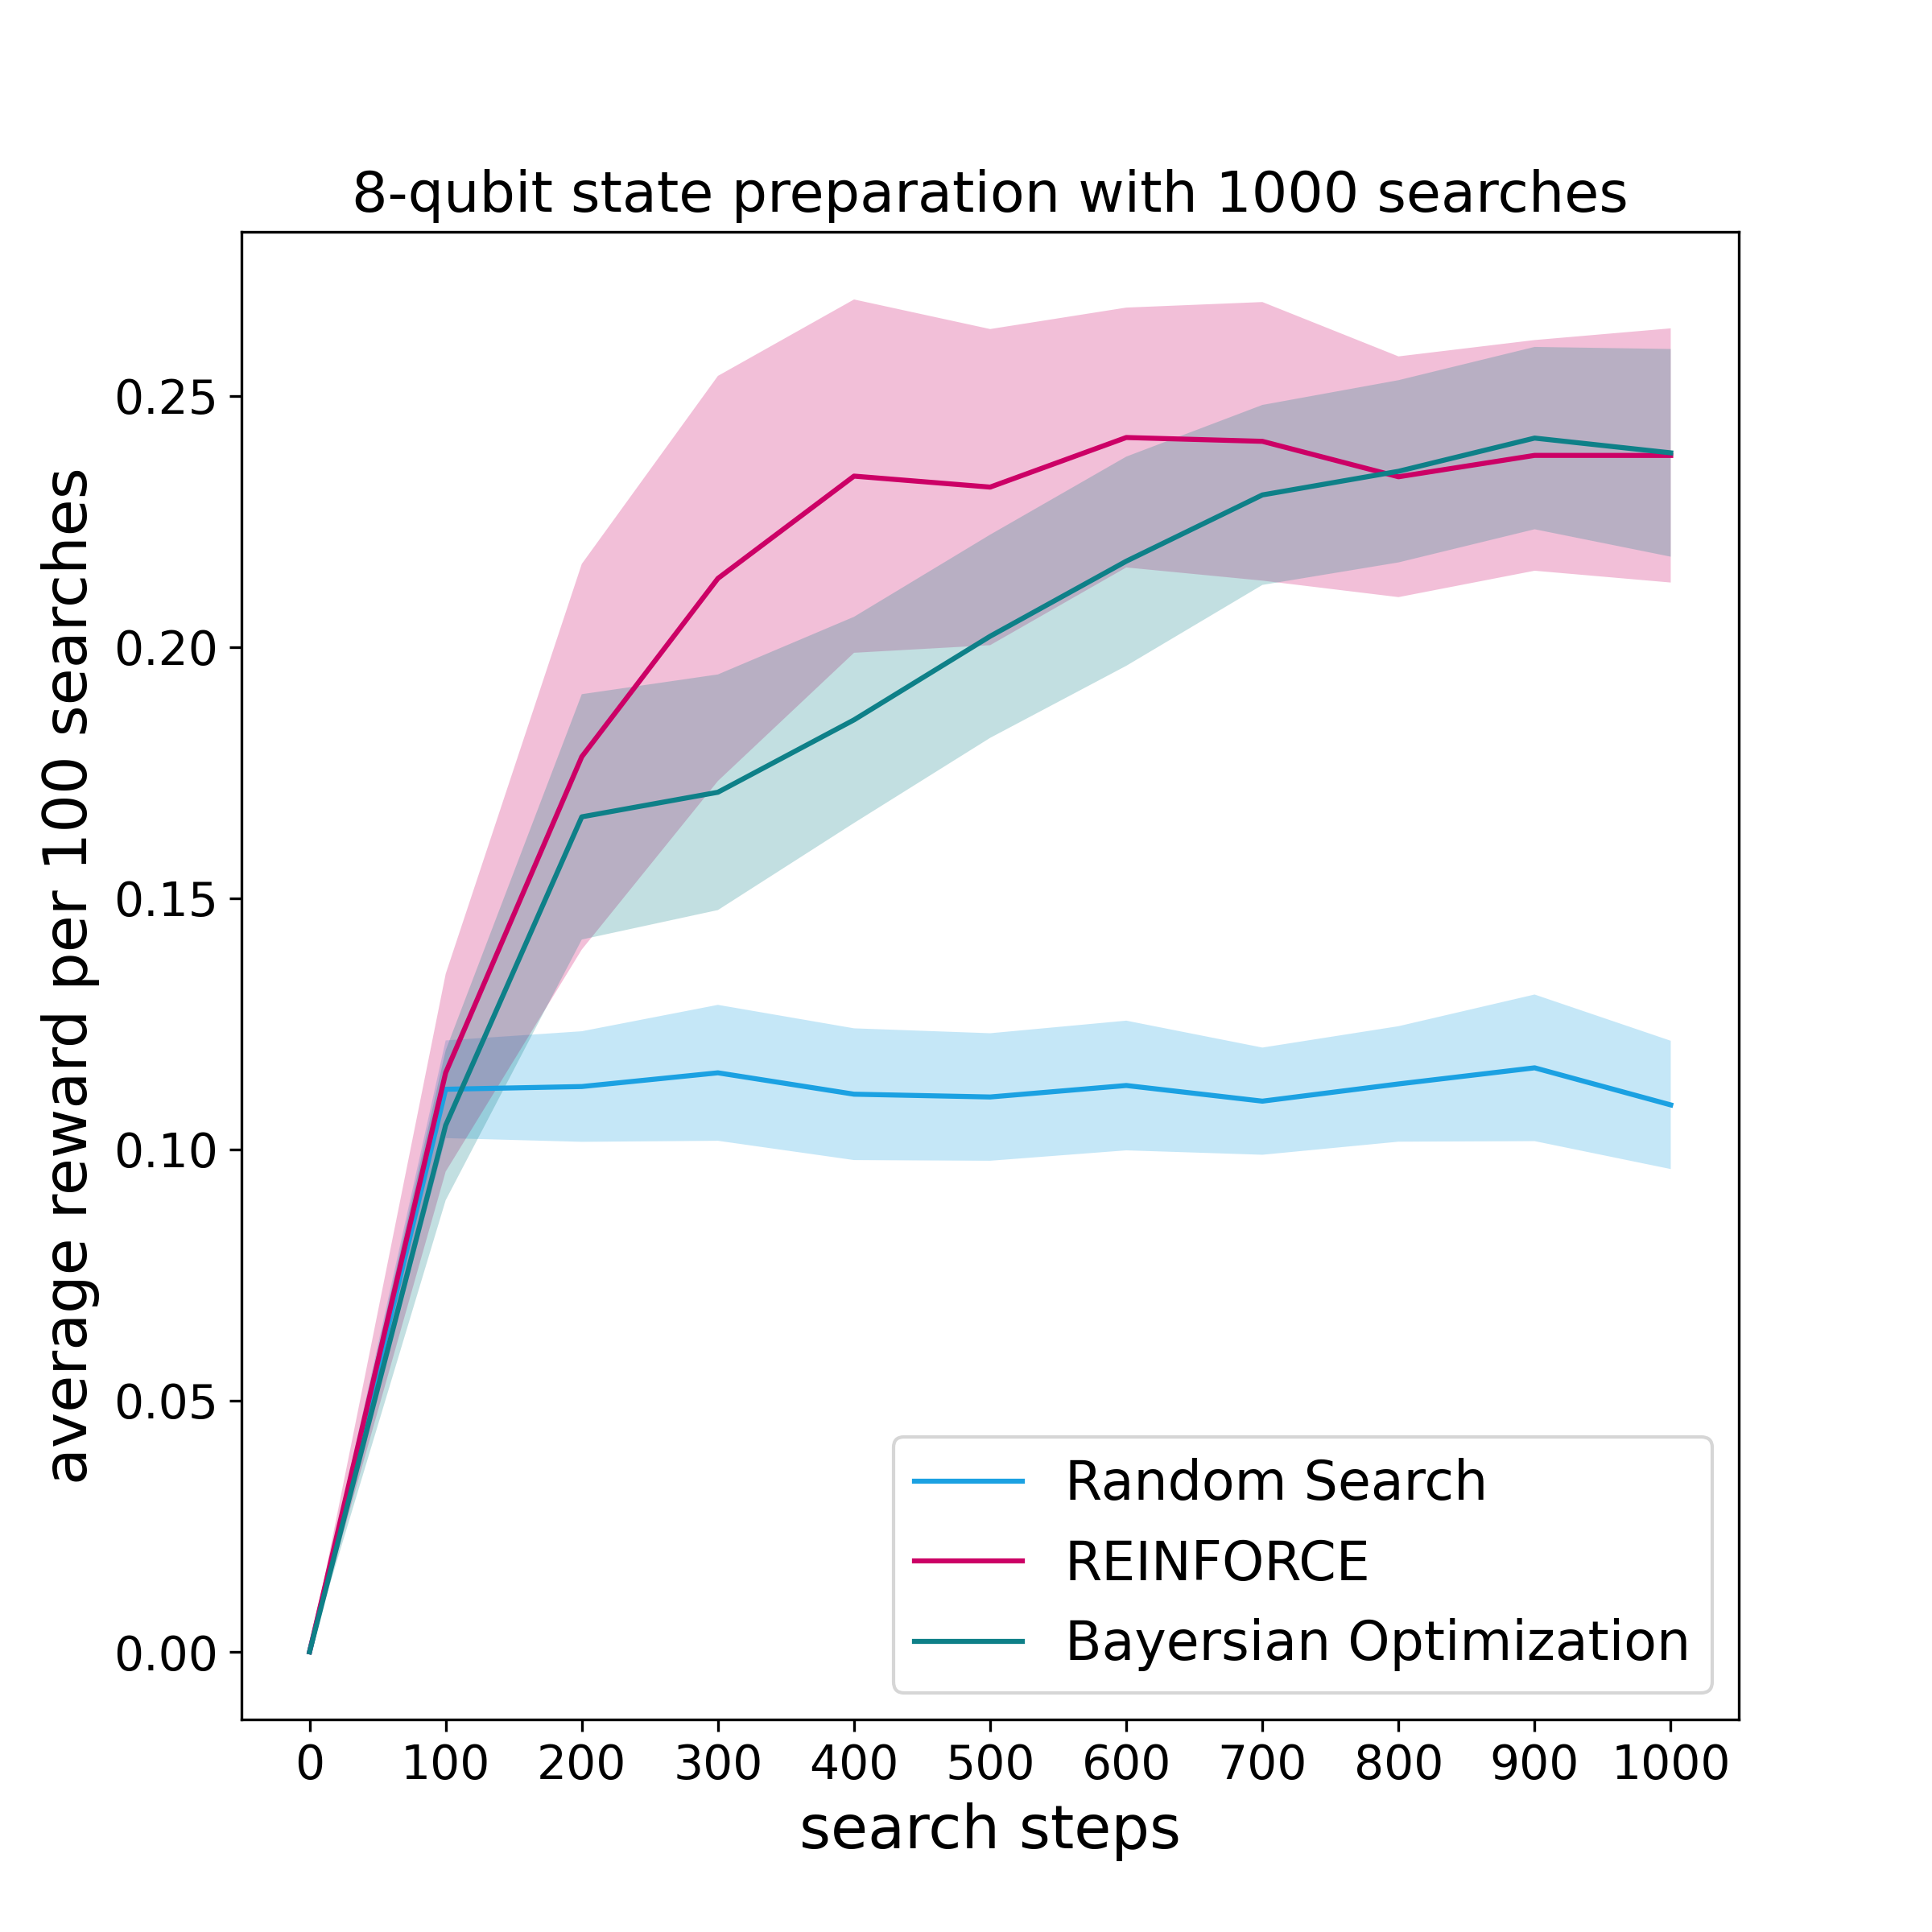
\includegraphics[width=0.49\textwidth]{images/8-qubits-fidelity_avg_reward_per_100_with_var_filling.png} %
    \includegraphics[width=0.49\textwidth]{images/8-qubits-fidelity_regret_fidelity_from_200_with_var_willing.png} %
    \caption{8-qubit state preparation}
    \label{8-qubit_fidelity}
    \end{subfigure}

    \begin{subfigure}[b]{0.49\textwidth}
    \centering
    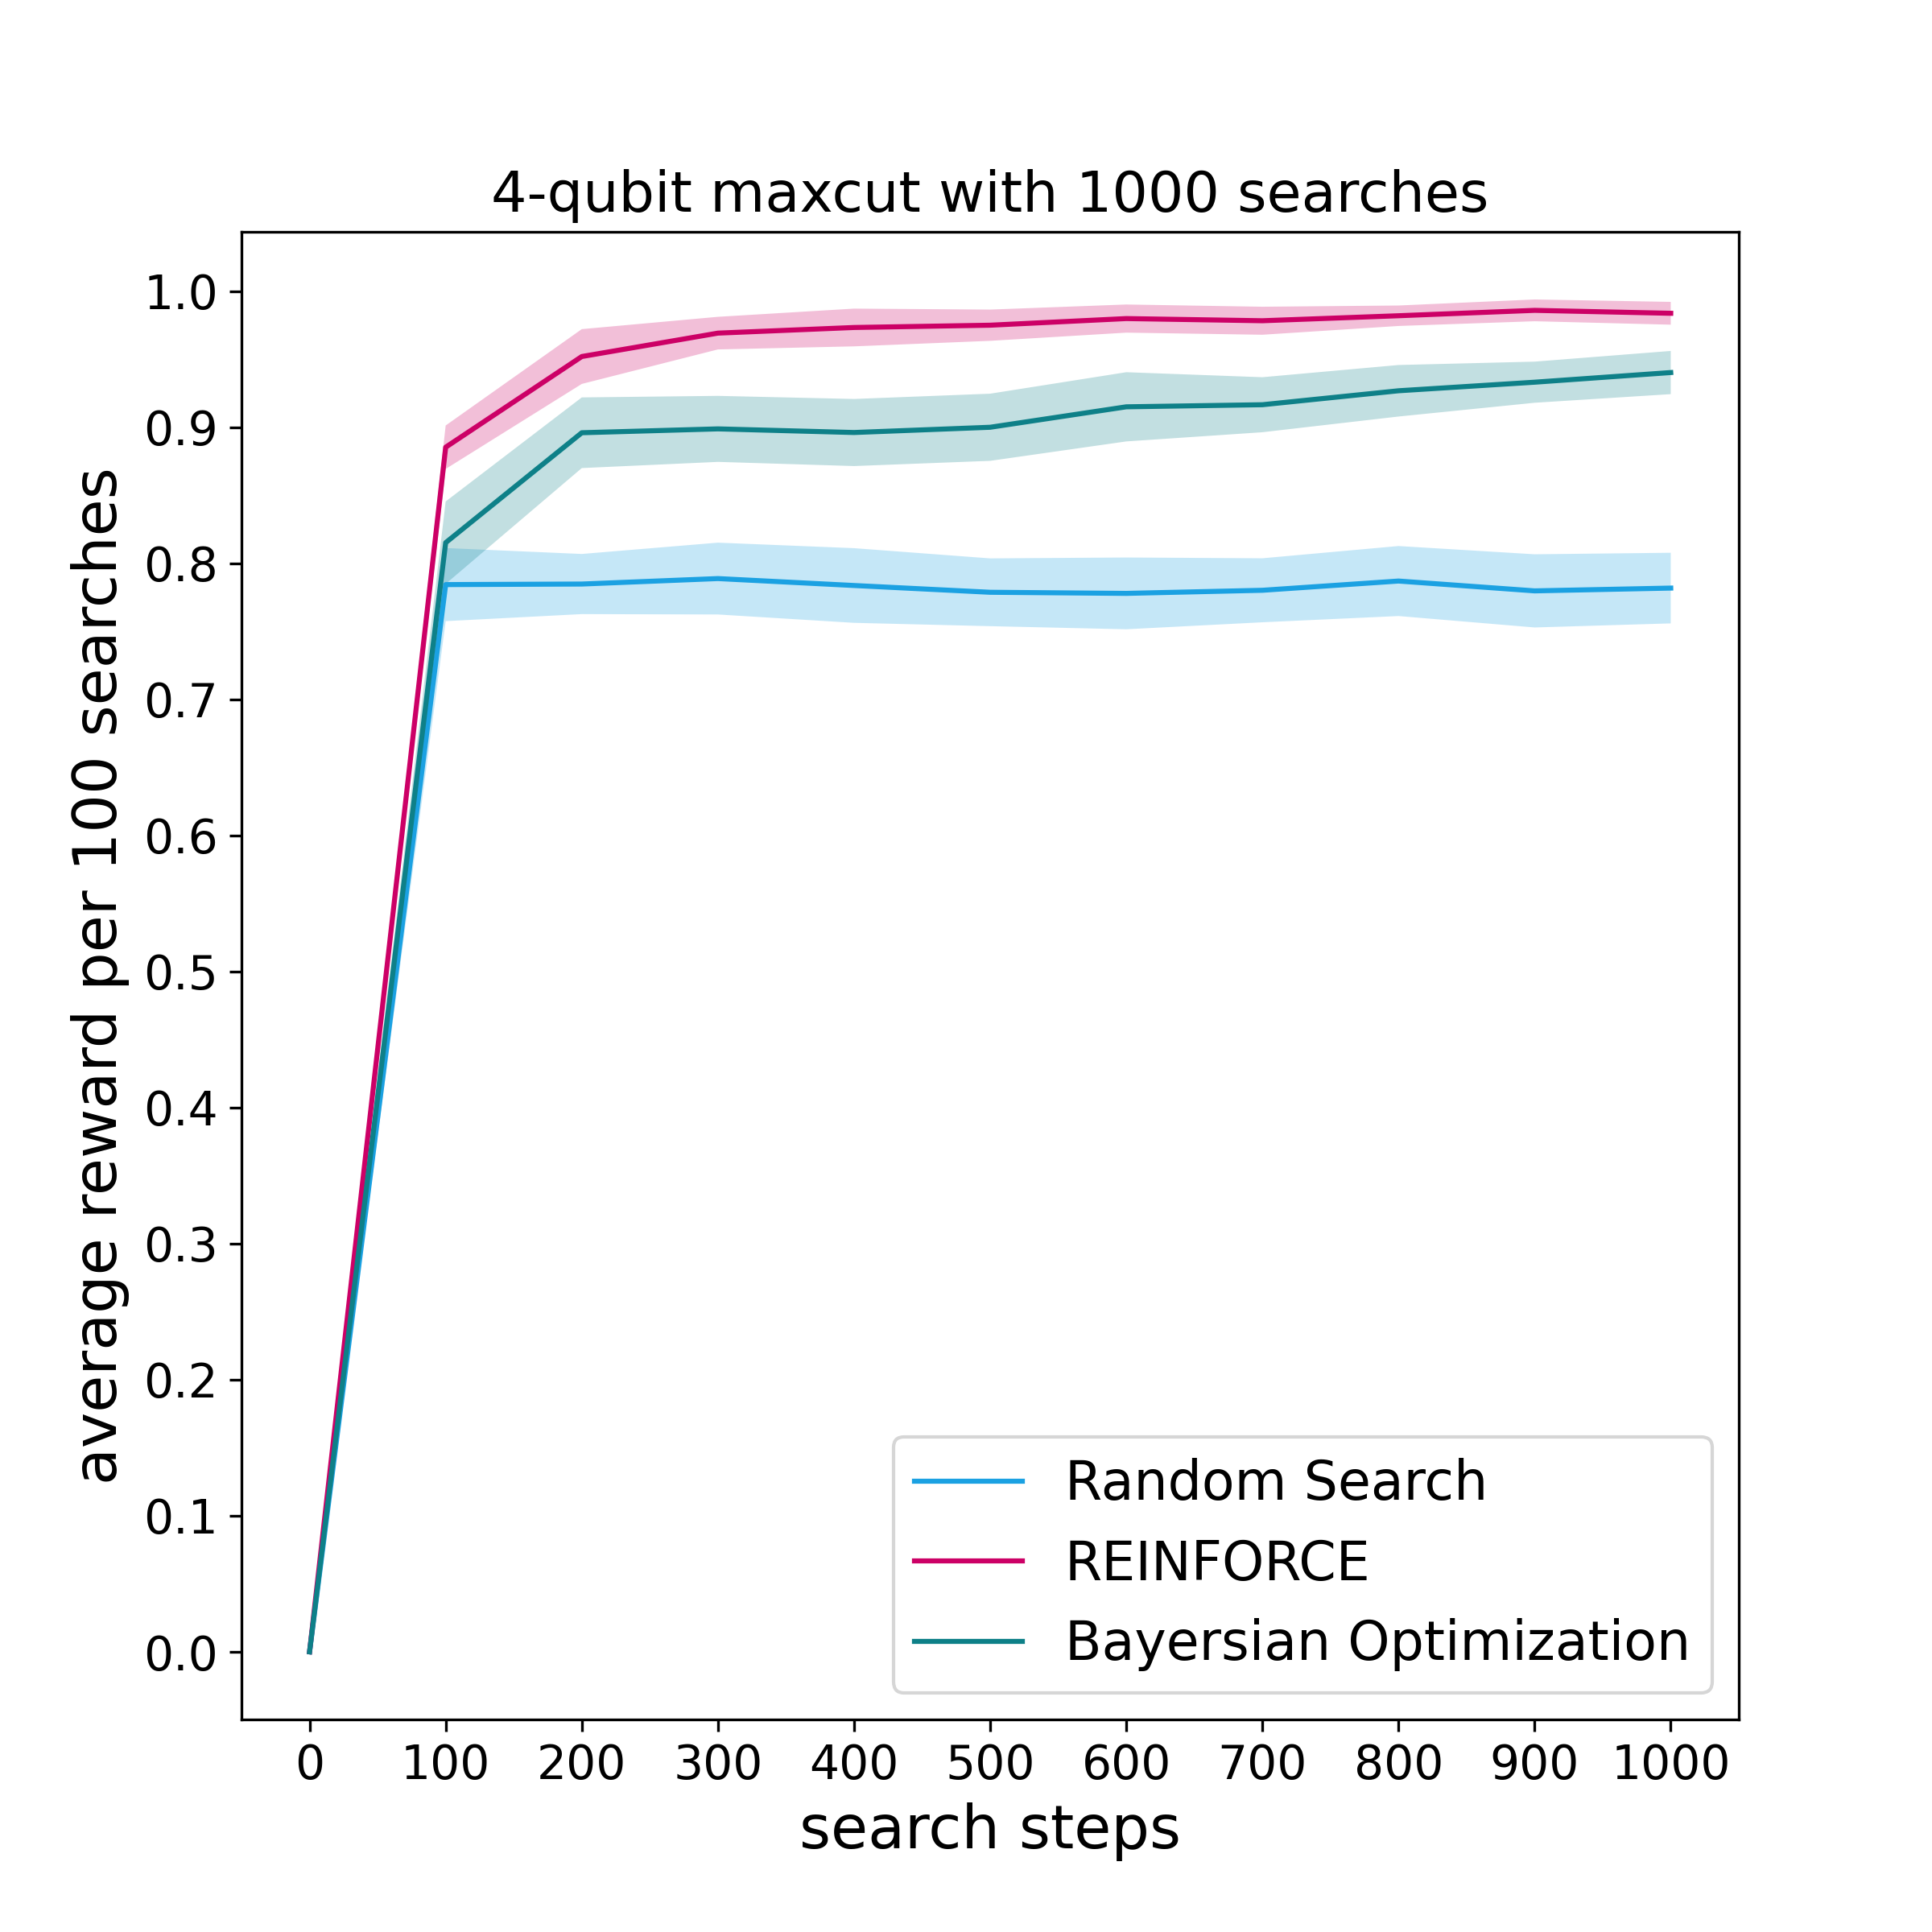
\includegraphics[width=0.49\textwidth]{images/4-qubits-maxcut_avg_reward_per_100_with_var_filling.png}
    \includegraphics[width=0.49\textwidth]{images/4-qubits-maxcut_regret_energy_from_100_with_var_willing.png}
    \caption{4-qubit max-cut} 
    \label{4-qubit_maxcut}
    \end{subfigure}
    \hfill
    \begin{subfigure}[b]{0.49\textwidth}
    \centering
    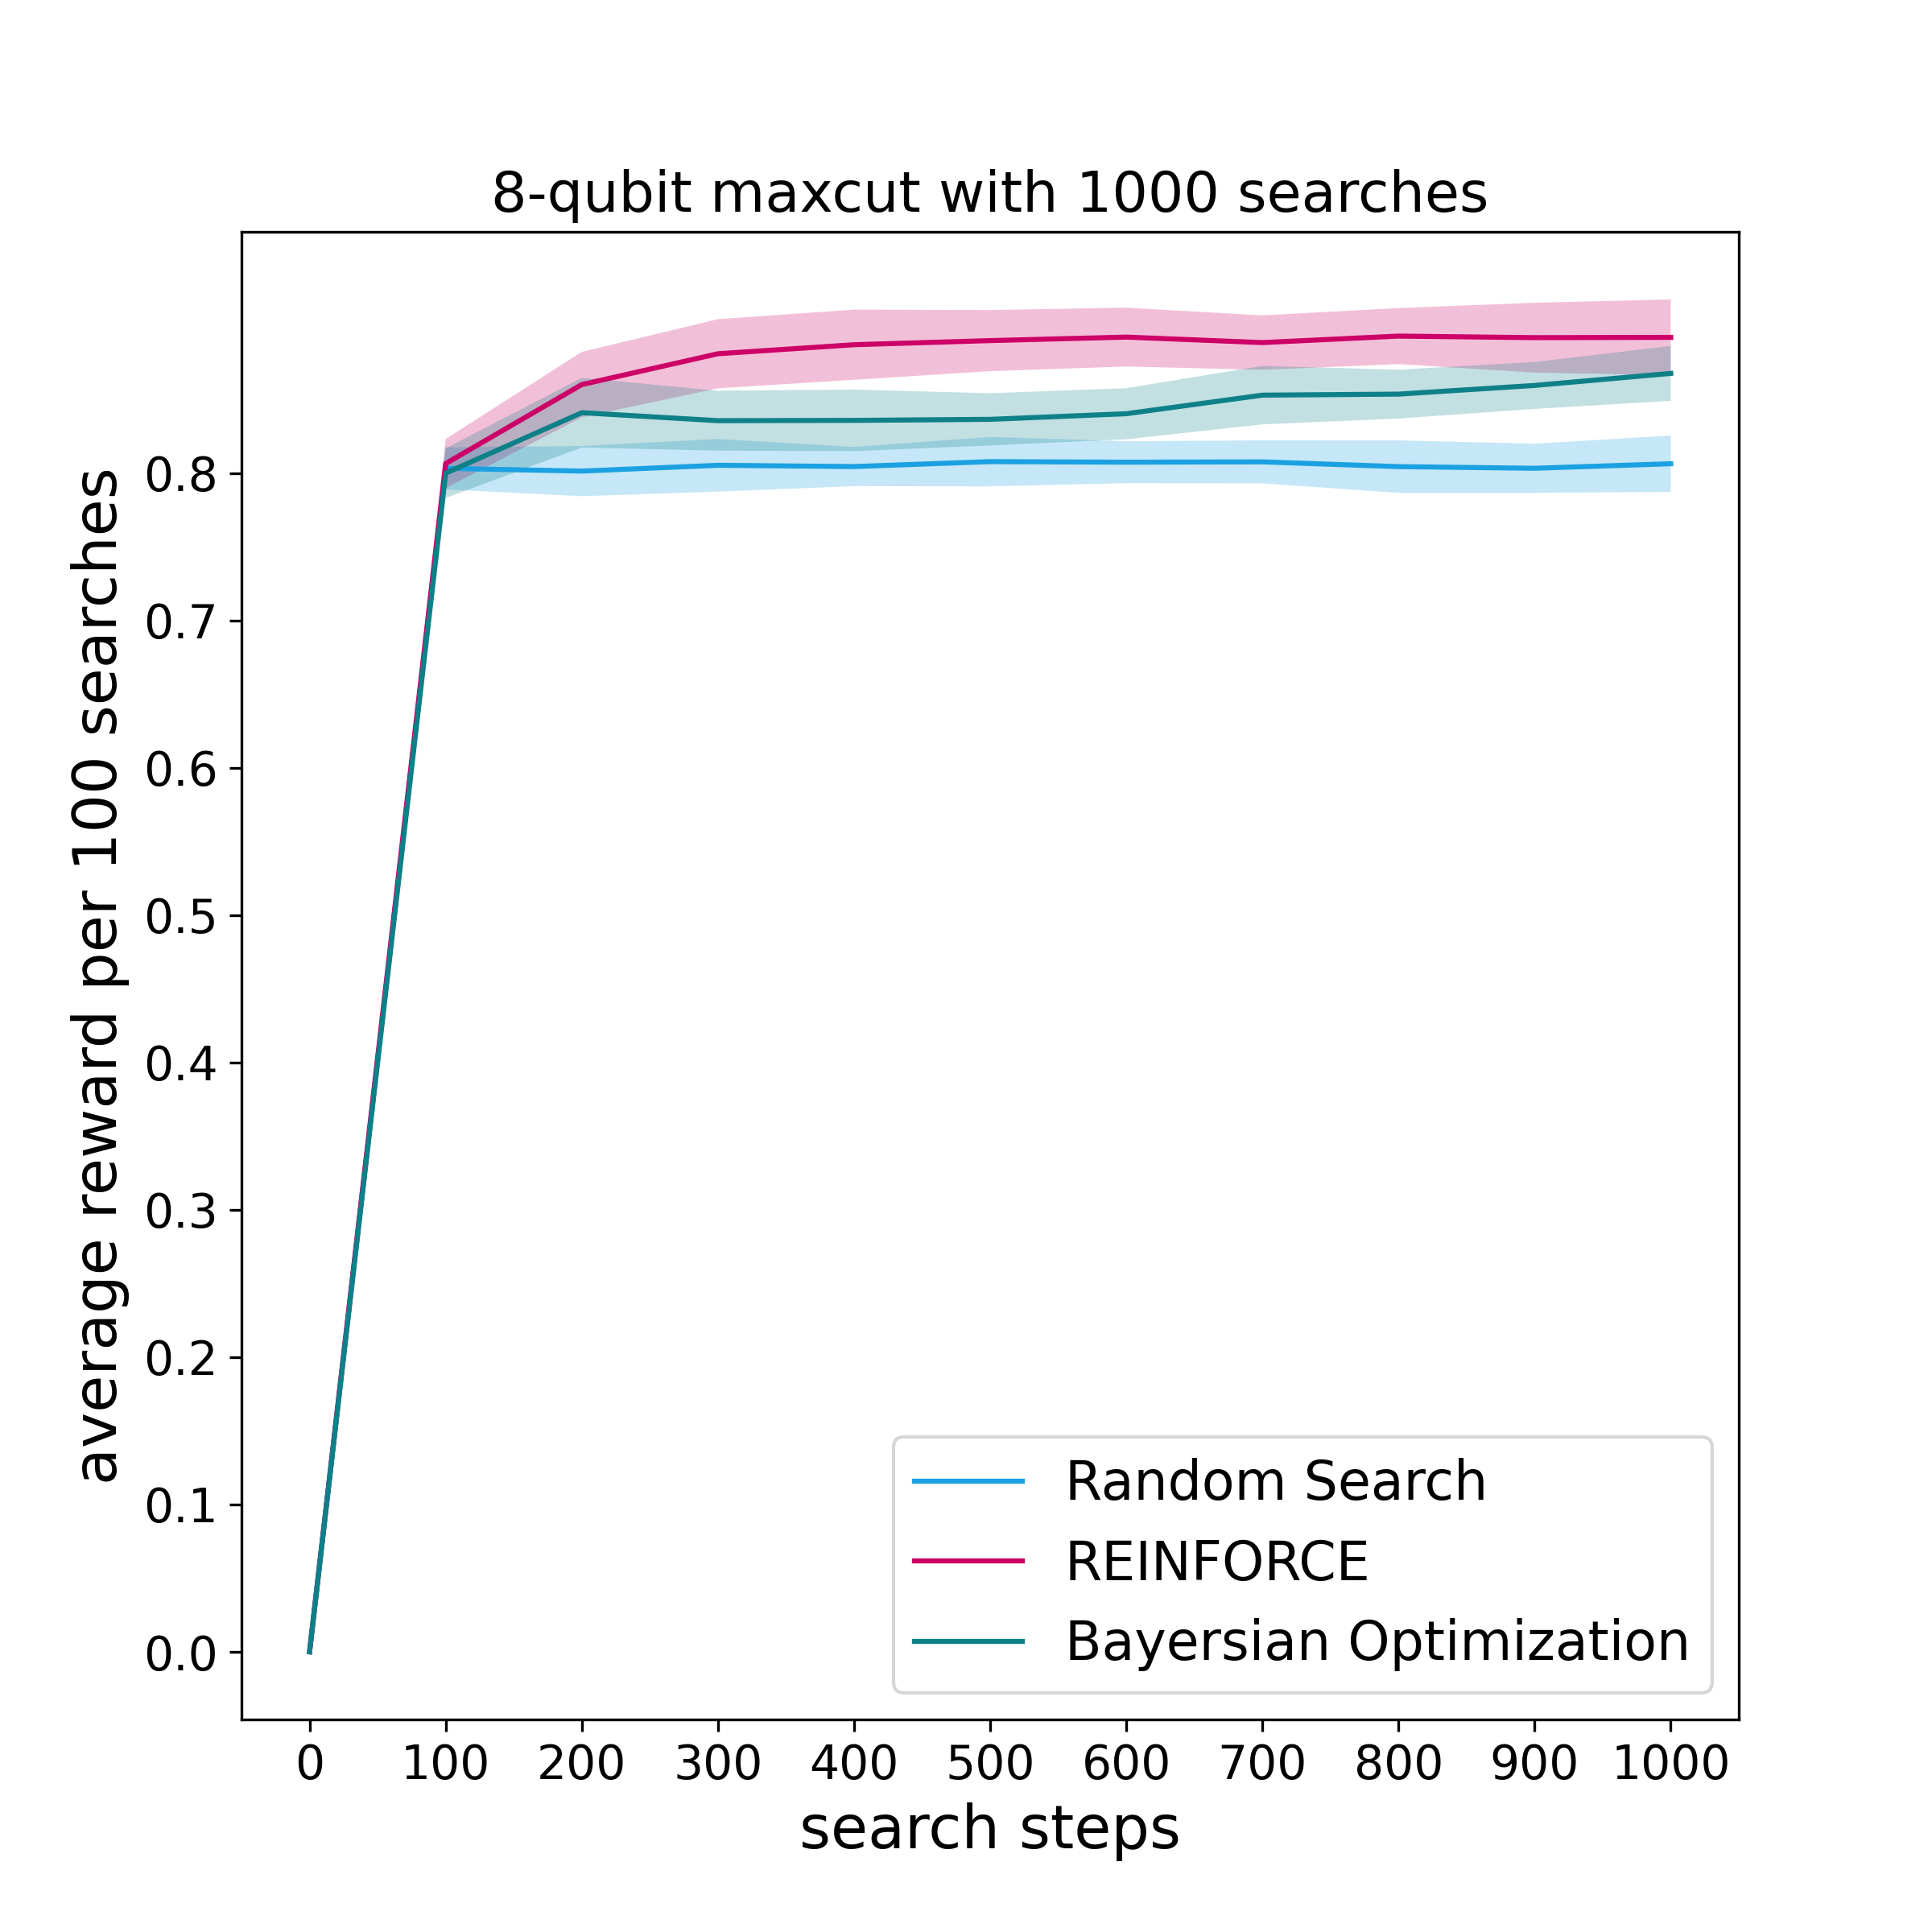
\includegraphics[width=0.49\textwidth]{images/8-qubits-maxcut_avg_reward_per_100_with_var_filling.png}
    \includegraphics[width=0.49\textwidth]{images/8-qubits-maxcut_regret_energy_from_100_with_var_willing.png}
    \caption{8-qubit max-cut} 
    \label{8-qubits_maxcut}
    \end{subfigure}
    
    \begin{subfigure}[b]{0.49\textwidth}
    \centering
    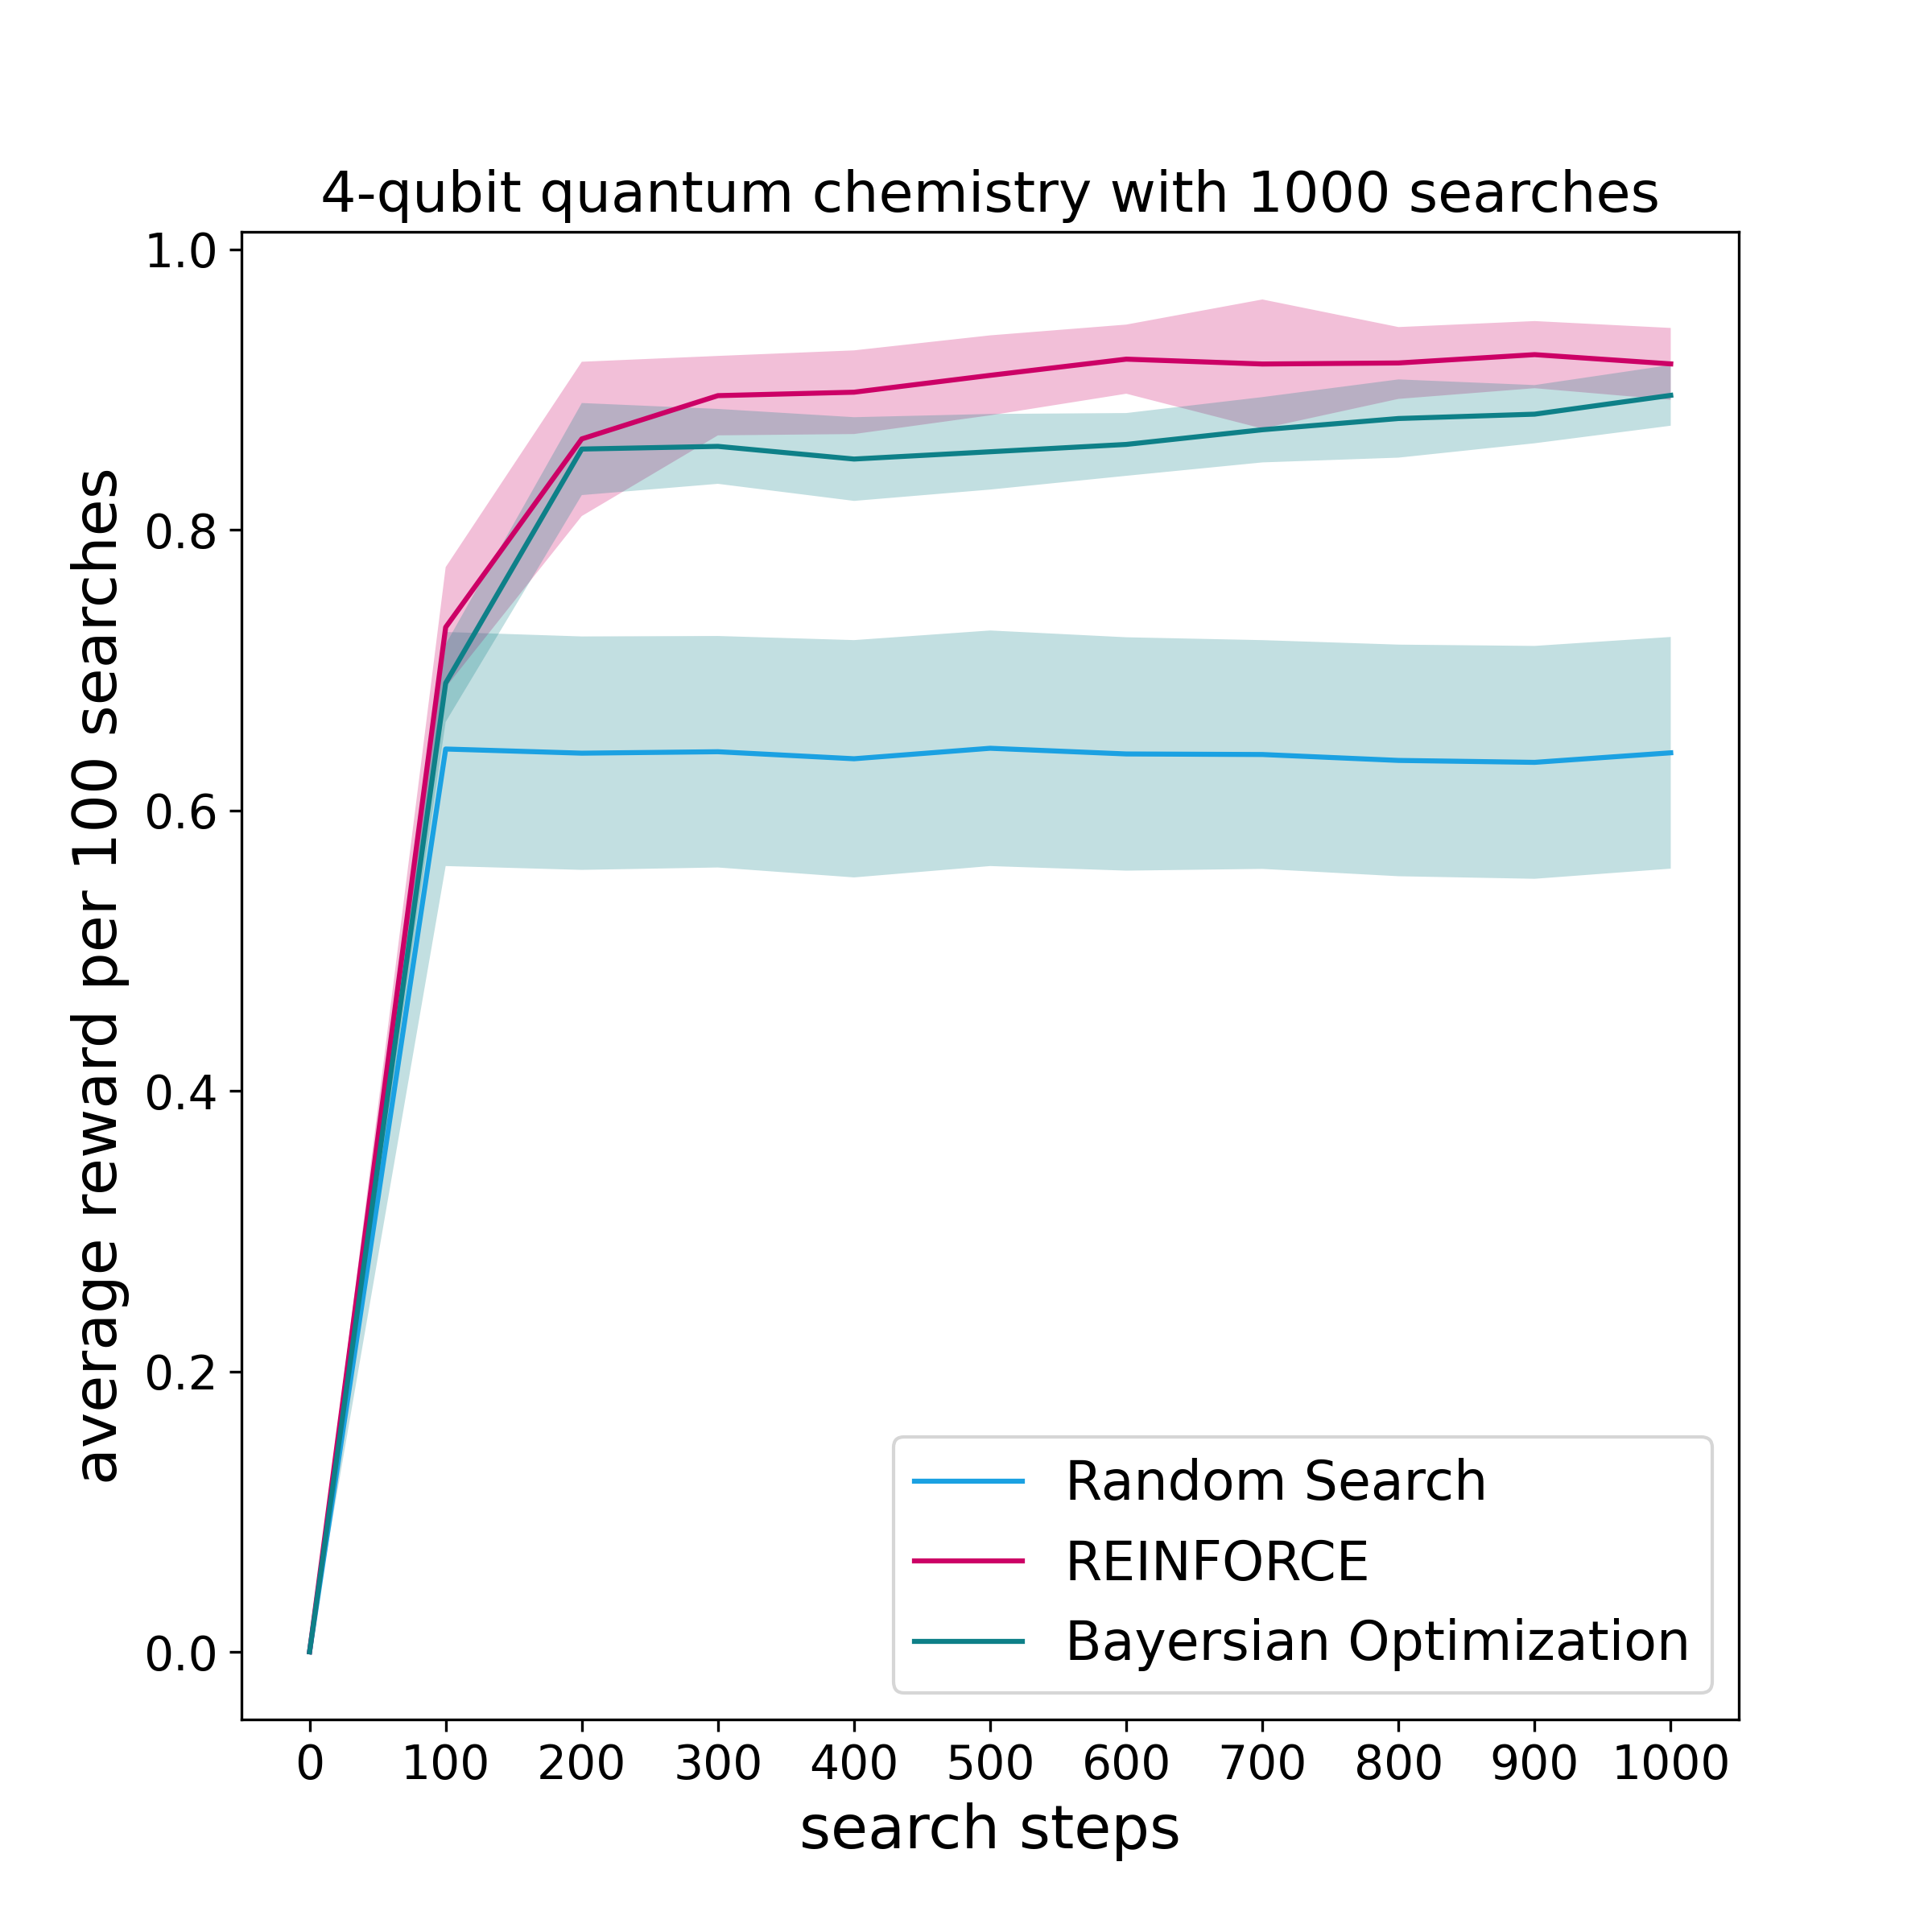
\includegraphics[width=0.49\textwidth]{images/4-qubits-vqe_avg_reward_per_100_with_var_filling.png}
    \includegraphics[width=0.49\textwidth]{images/4-qubits-vqe_regret_energy_from_100_with_var_willing.png}
    \caption{4-qubit quantum chemistry} 
    \label{4-qubit_vqe}
    \end{subfigure}
    \hfill
    \begin{subfigure}[b]{0.49\textwidth}
    \centering
    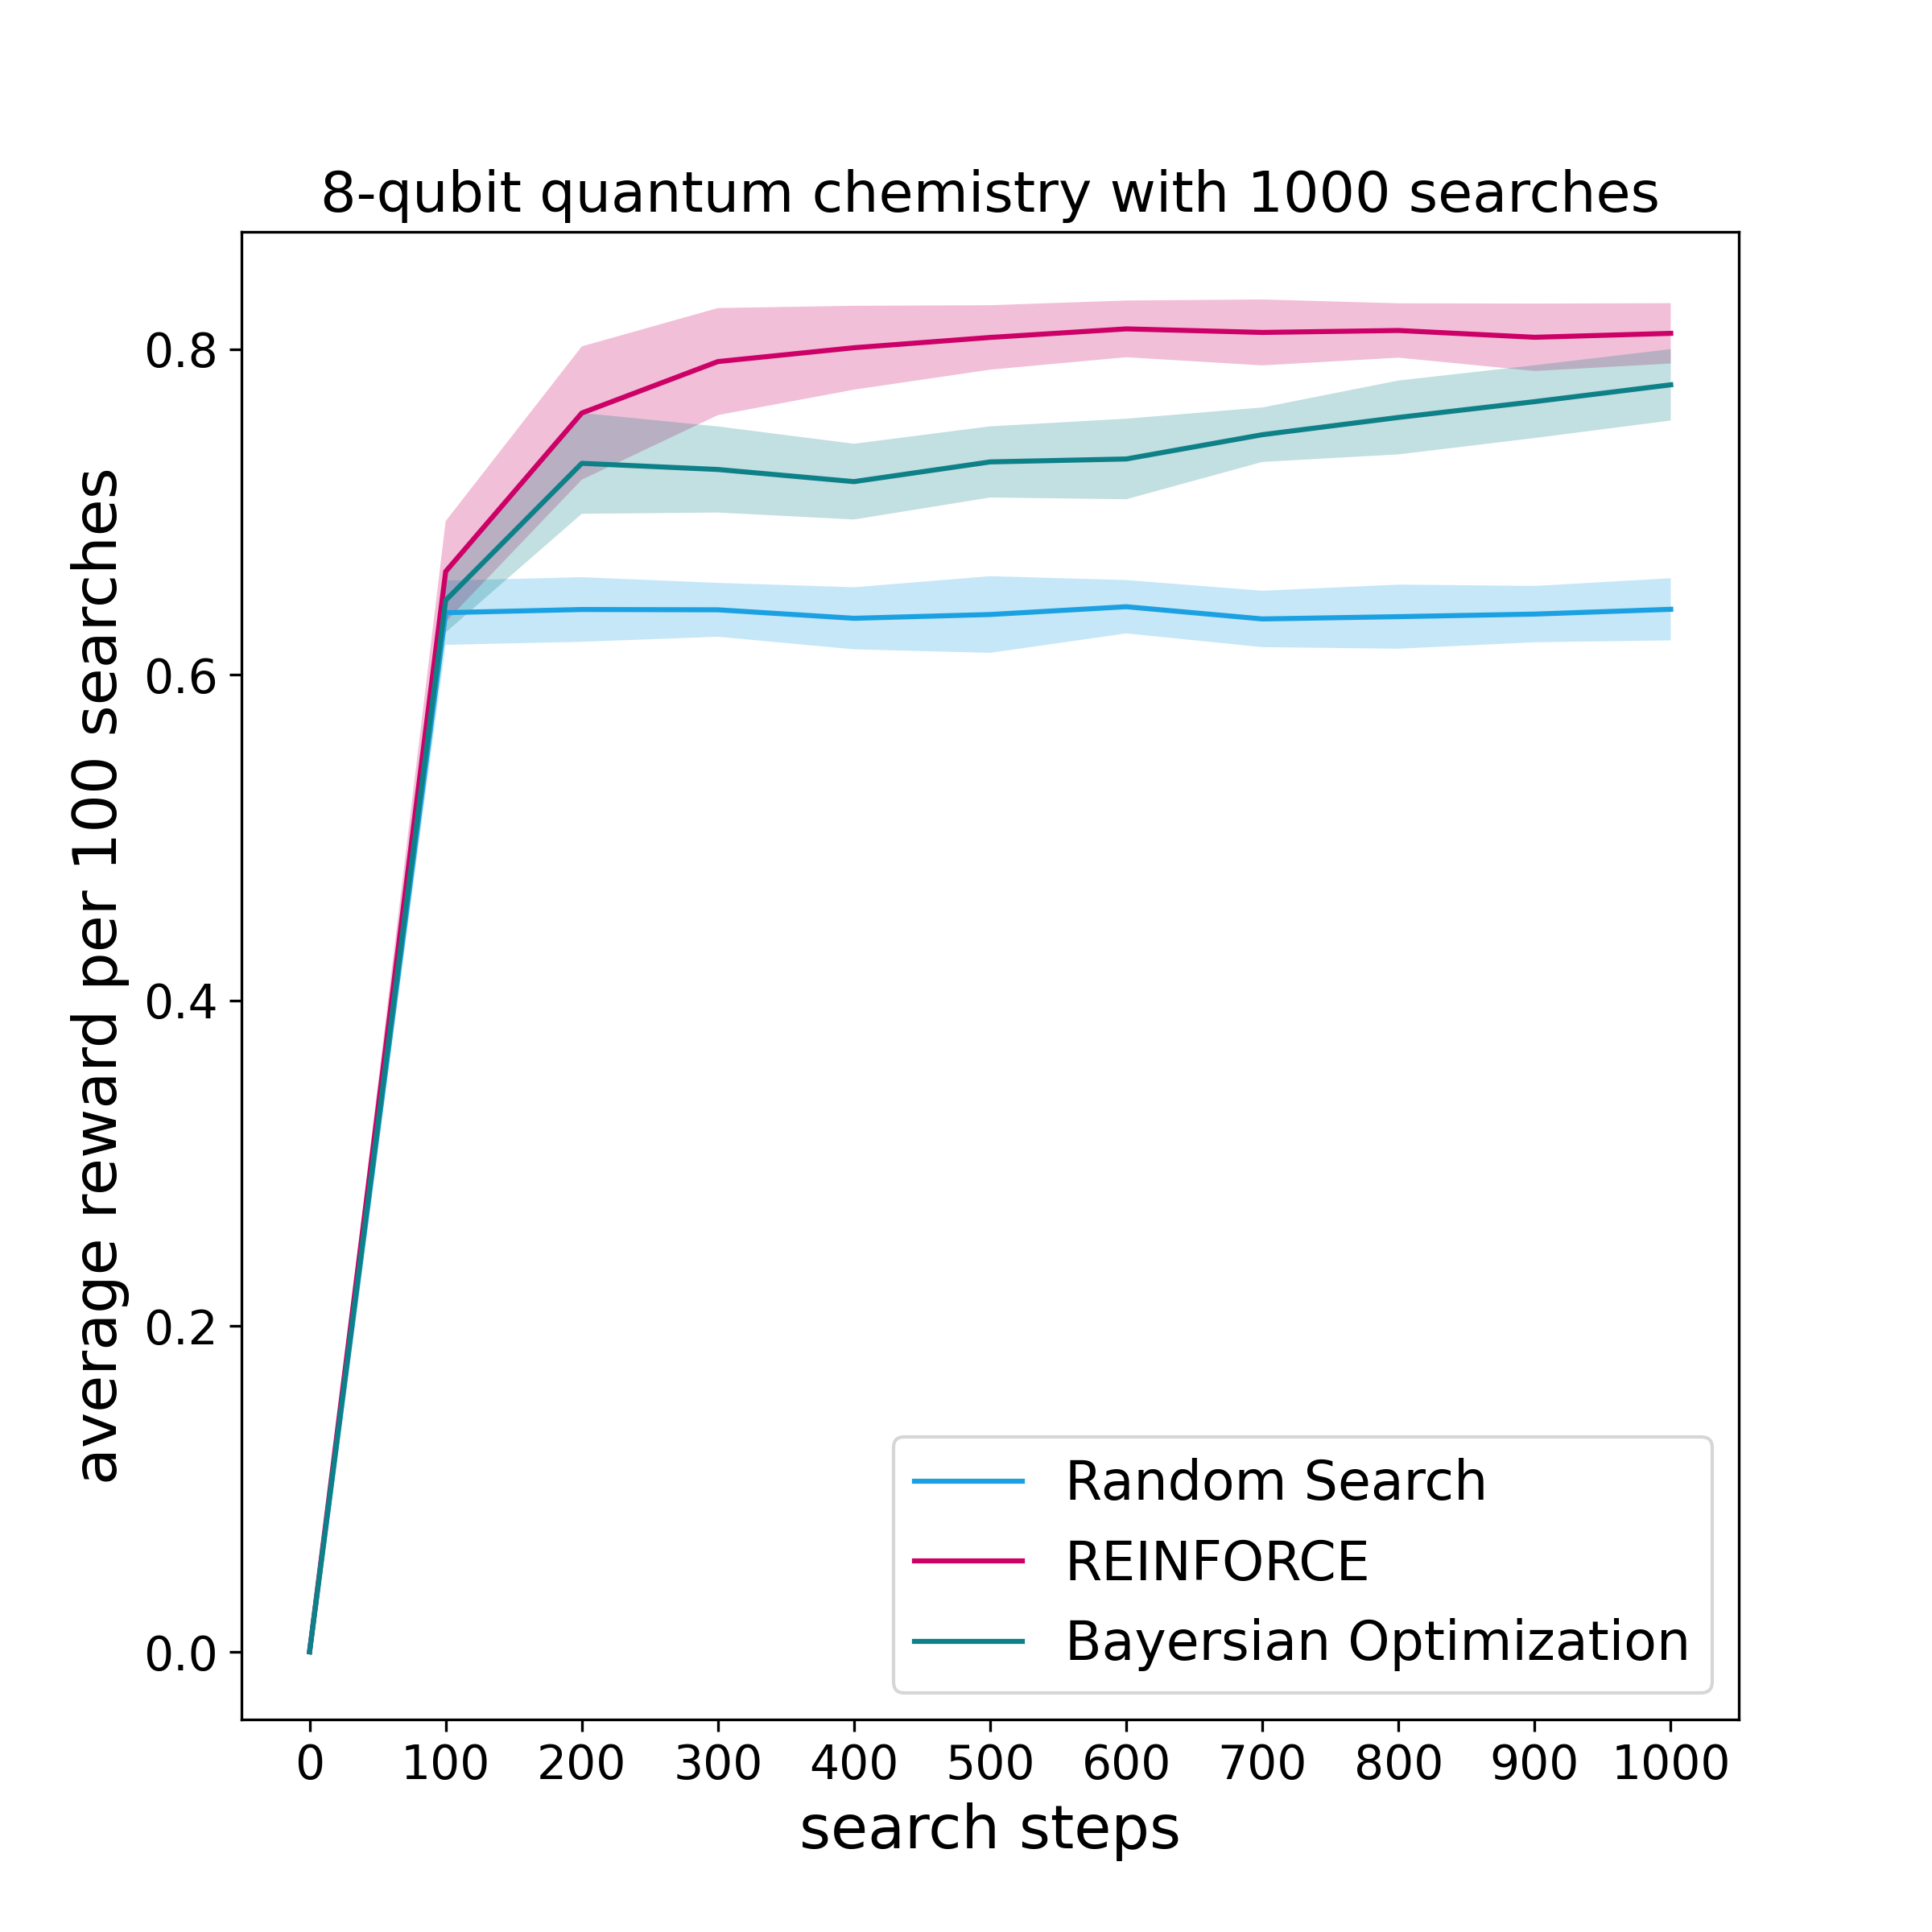
\includegraphics[width=0.49\textwidth]{images/8-qubits-vqe_avg_reward_per_100_with_var_filling.png}
    \includegraphics[width=0.49\textwidth]{images/8-qubits-vqe_regret_energy_from_100_with_var_willing.png}
    \caption{8-qubit quantum chemistry} 
    \label{8-qubits_vqe}
    \end{subfigure}
    \caption{Average rewards and regret values of the 6 sets of experiments. The left side is the 4-qubit experiments and the right side is the 8-qubit experiments. In each set of experiments, the left plot shows the average reward and the right one shows the regret value. The left plots in each set of experiments show the average reward of 50 independent runs (with different random seeds) given 1000 search queries. The right plots in each set of experiments show the mean regret of 50 independent runs (with different random seeds) given 1000 search queries. The shaded areas in the plots demonstrate the standard deviation of the average rewards and the regret values respectively.}
    \label{average_reward_and_regret}
\end{center}
\end{figure}
\end{comment}

\textbf{Observation (2):} In Figure \ref{candidates}, we illustrate the number of candidate circuits found to achieve a preset threshold after performing 1000 searches using the three search methods. The results show that the 8-qubit experiments are more complex, resulting in fewer circuits meeting the requirements within the search space. Additionally, within a limited number of search iterations, both the REINFORCE and BO methods are able to discover a greater number of candidate circuits that meet the threshold, even in the worst case, i.e., when comparing the minimal number of candidates. Notably, their performance significantly surpasses that of the Random Search method, especially REINFORCE, despite the fact that the difference between the minimal and maximal number of candidates indicates that REINFORCE is more sensitive to the initial conditions compared to the other two approaches. These findings highlight the clear improvements and advantages introduced by QAS based on the latent representation, which enables the efficient discovery of numerous high-performance candidate circuits while reducing the number of searches required.
\begin{figure}[htbp]
    \centering
    % Left side (a)
    \begin{subfigure}[b]{0.48\textwidth}
        \centering
        \begin{minipage}[b]{0.7\textwidth}
            \centering
            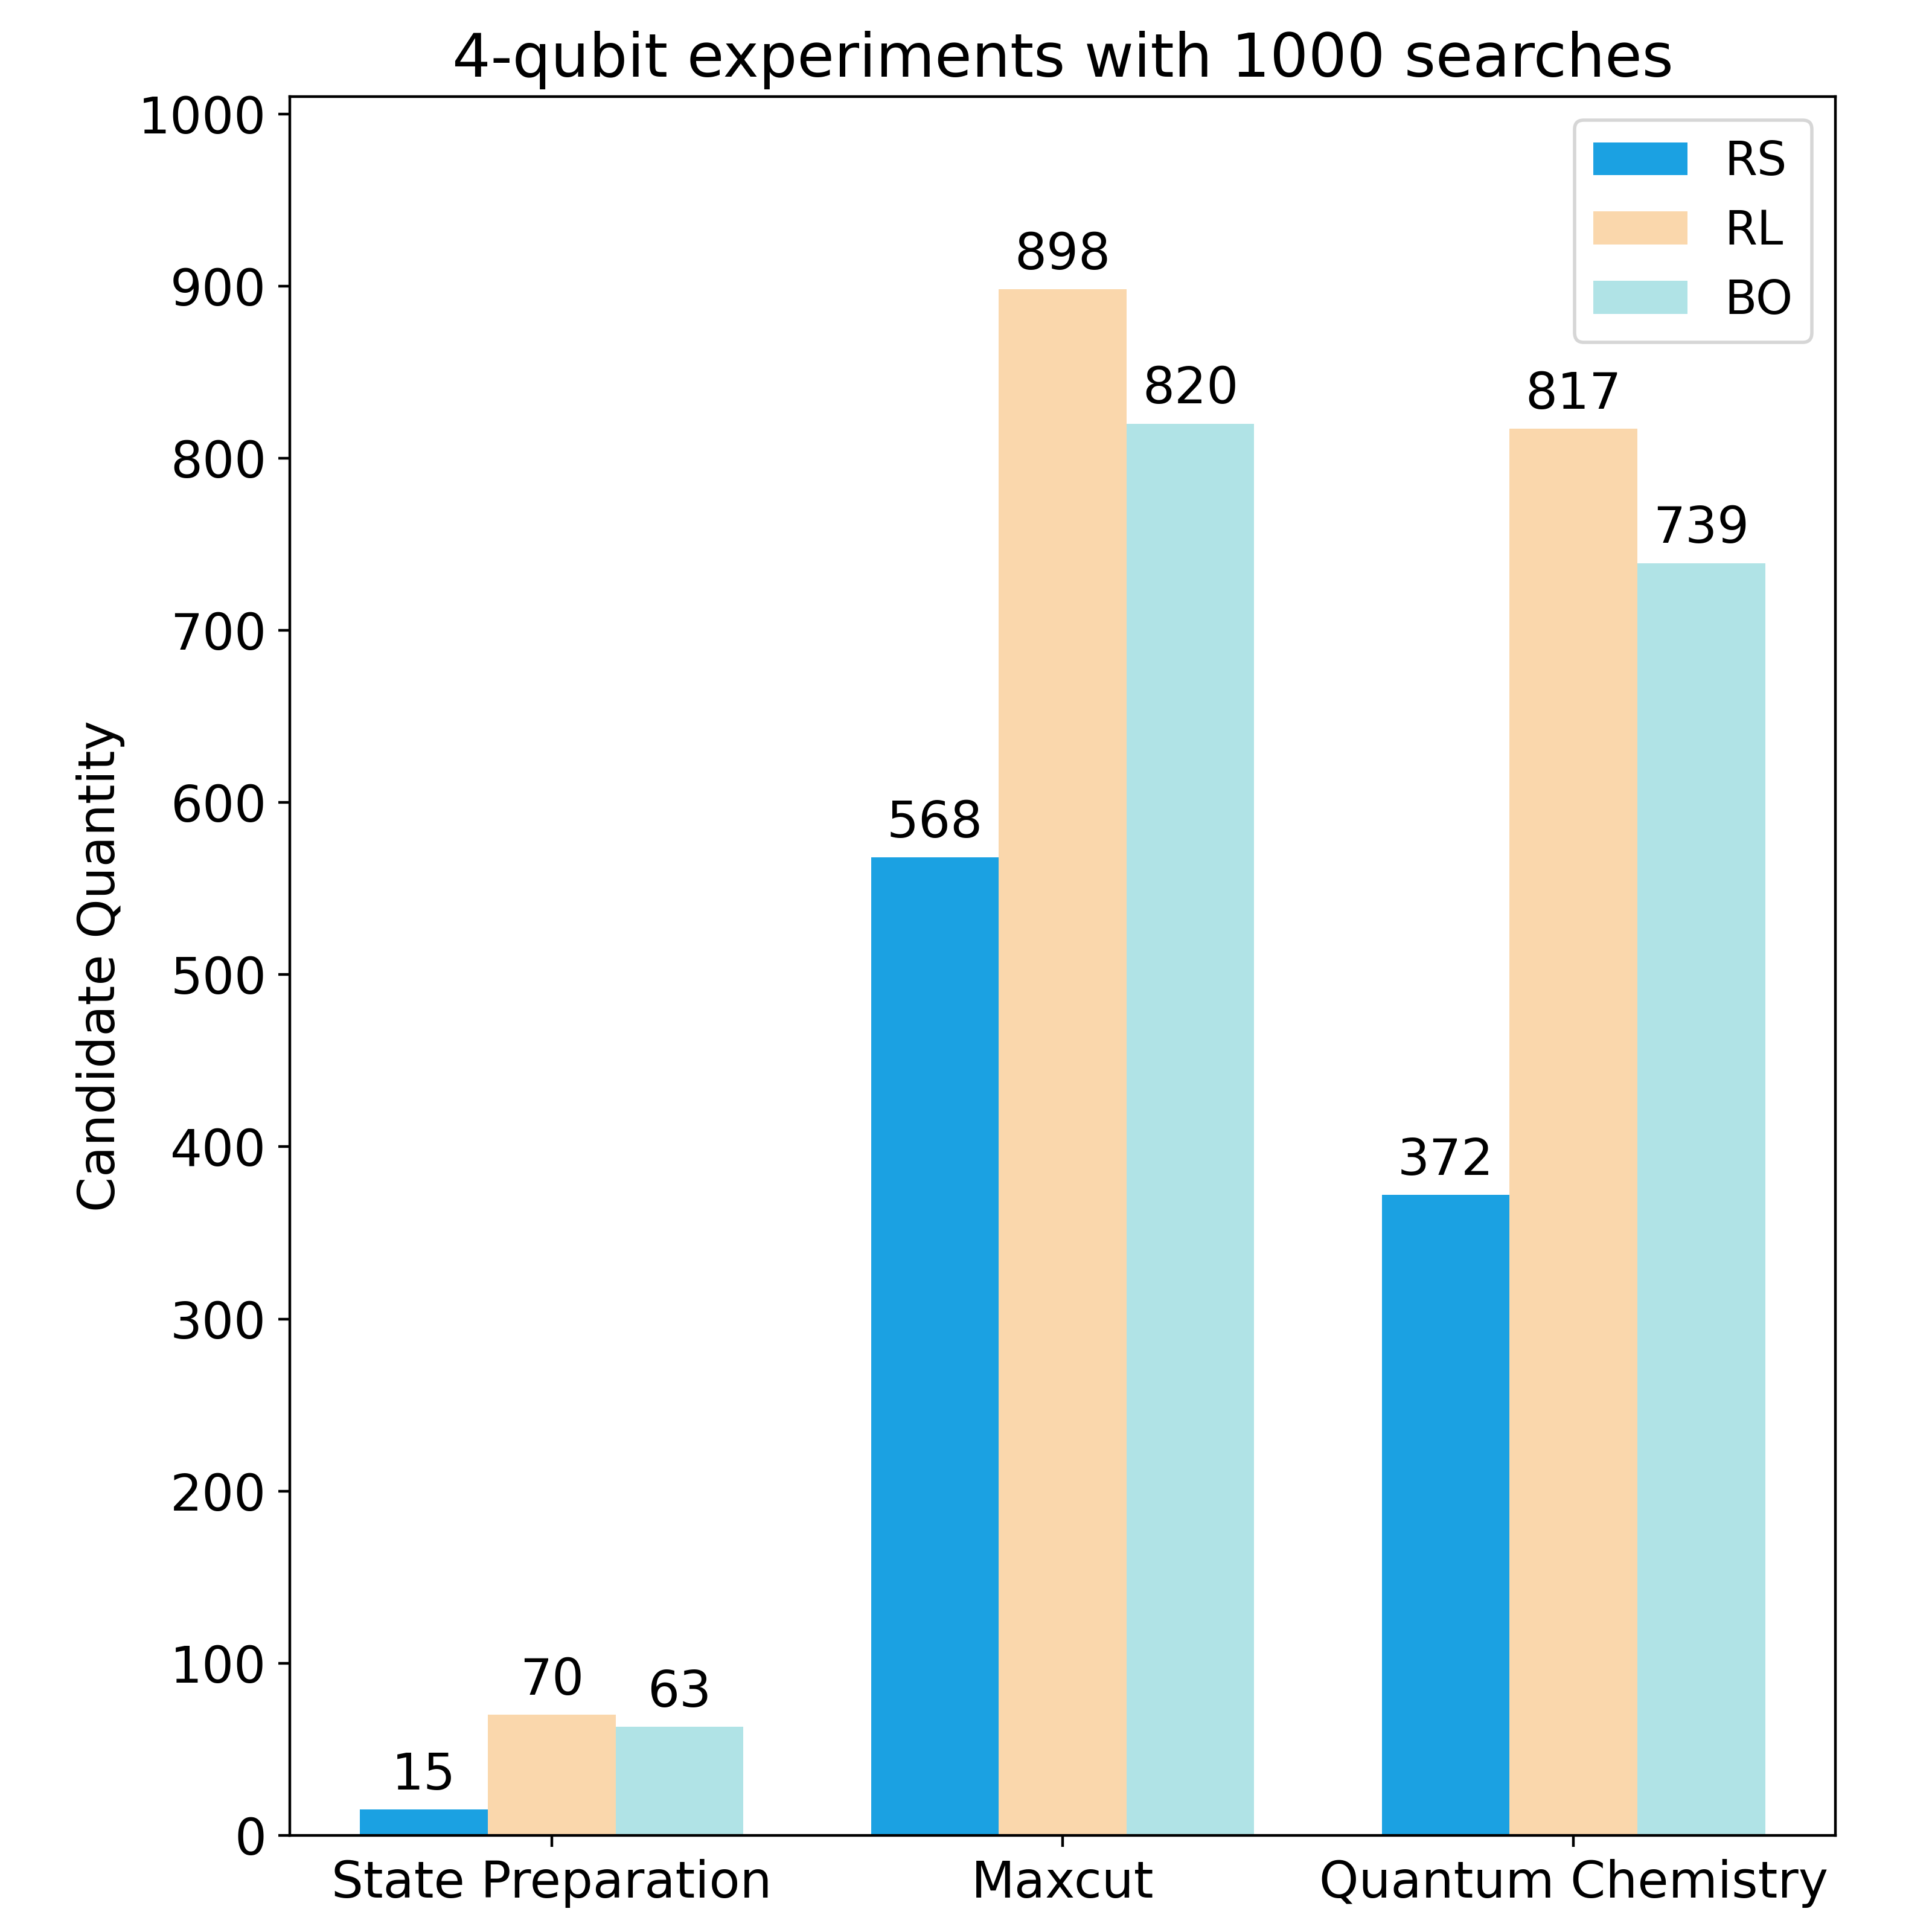
\includegraphics[width=0.8\textwidth]{images/4-qubits_experiments_candidates.png}
        \end{minipage}
        \hspace{-1em}
        \begin{minipage}[b]{0.28\textwidth}
            \centering
            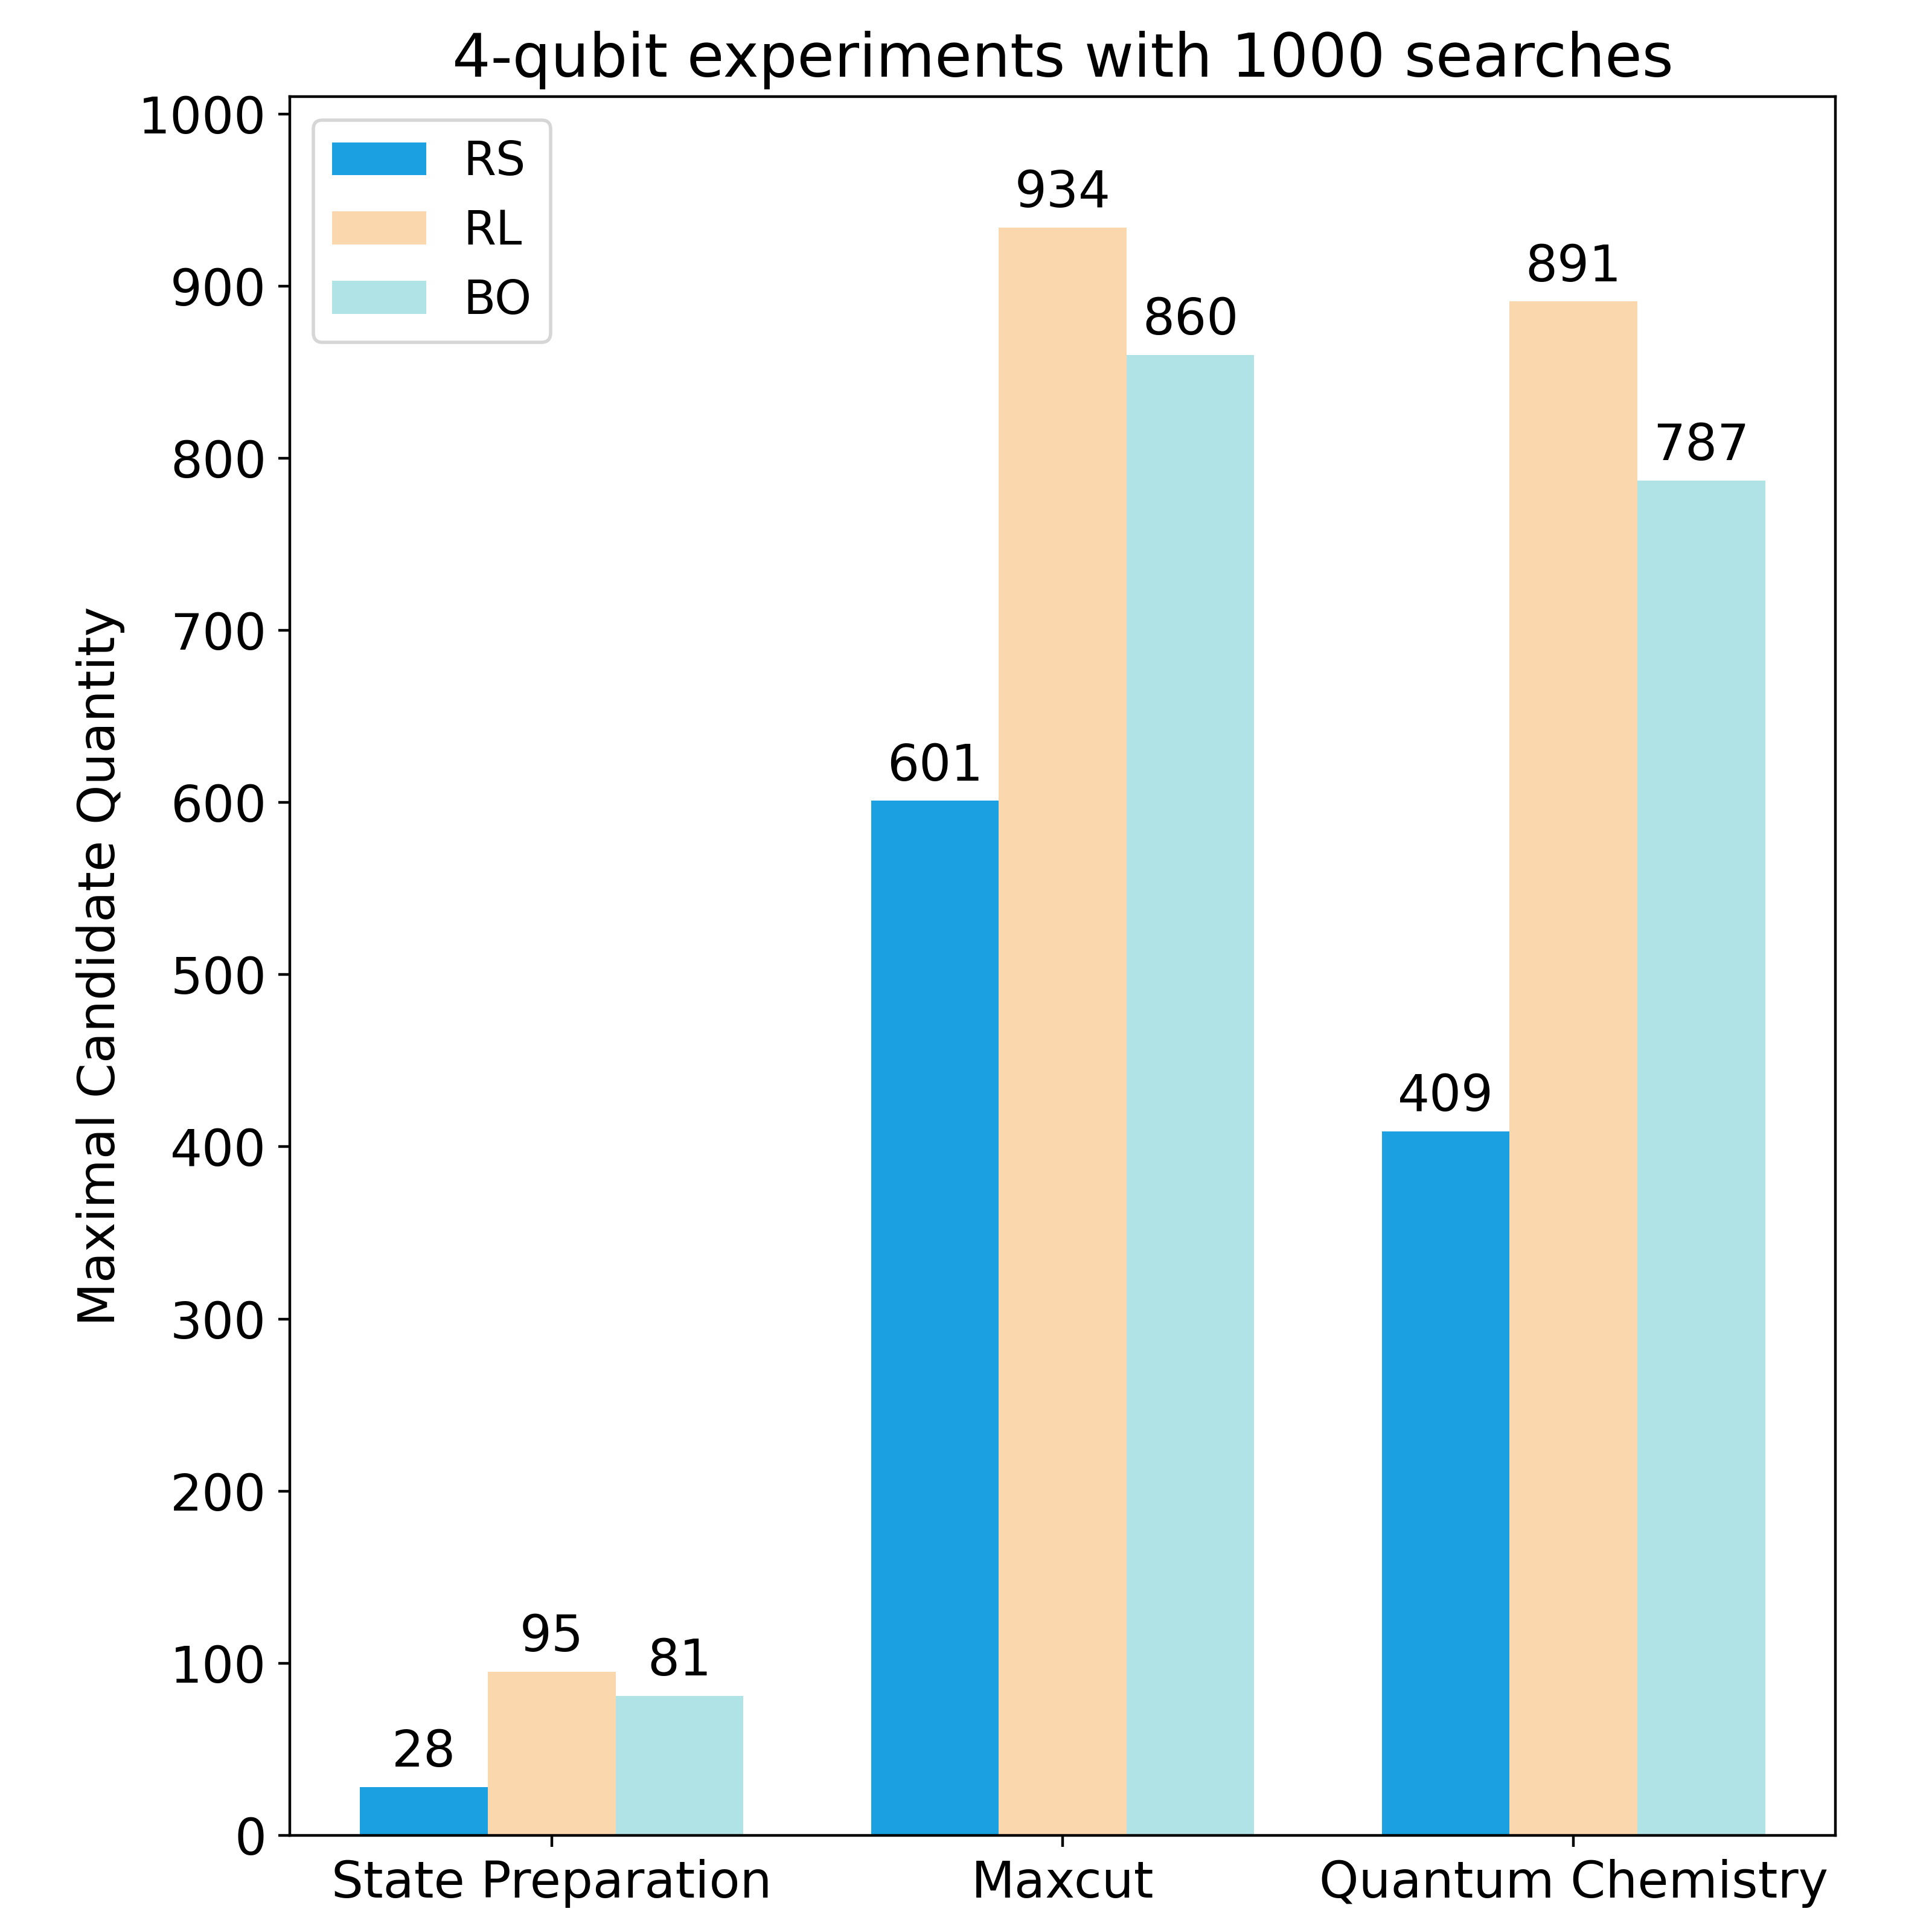
\includegraphics[width=\textwidth]{images/4-qubits_experiments_candidates_max.png}
            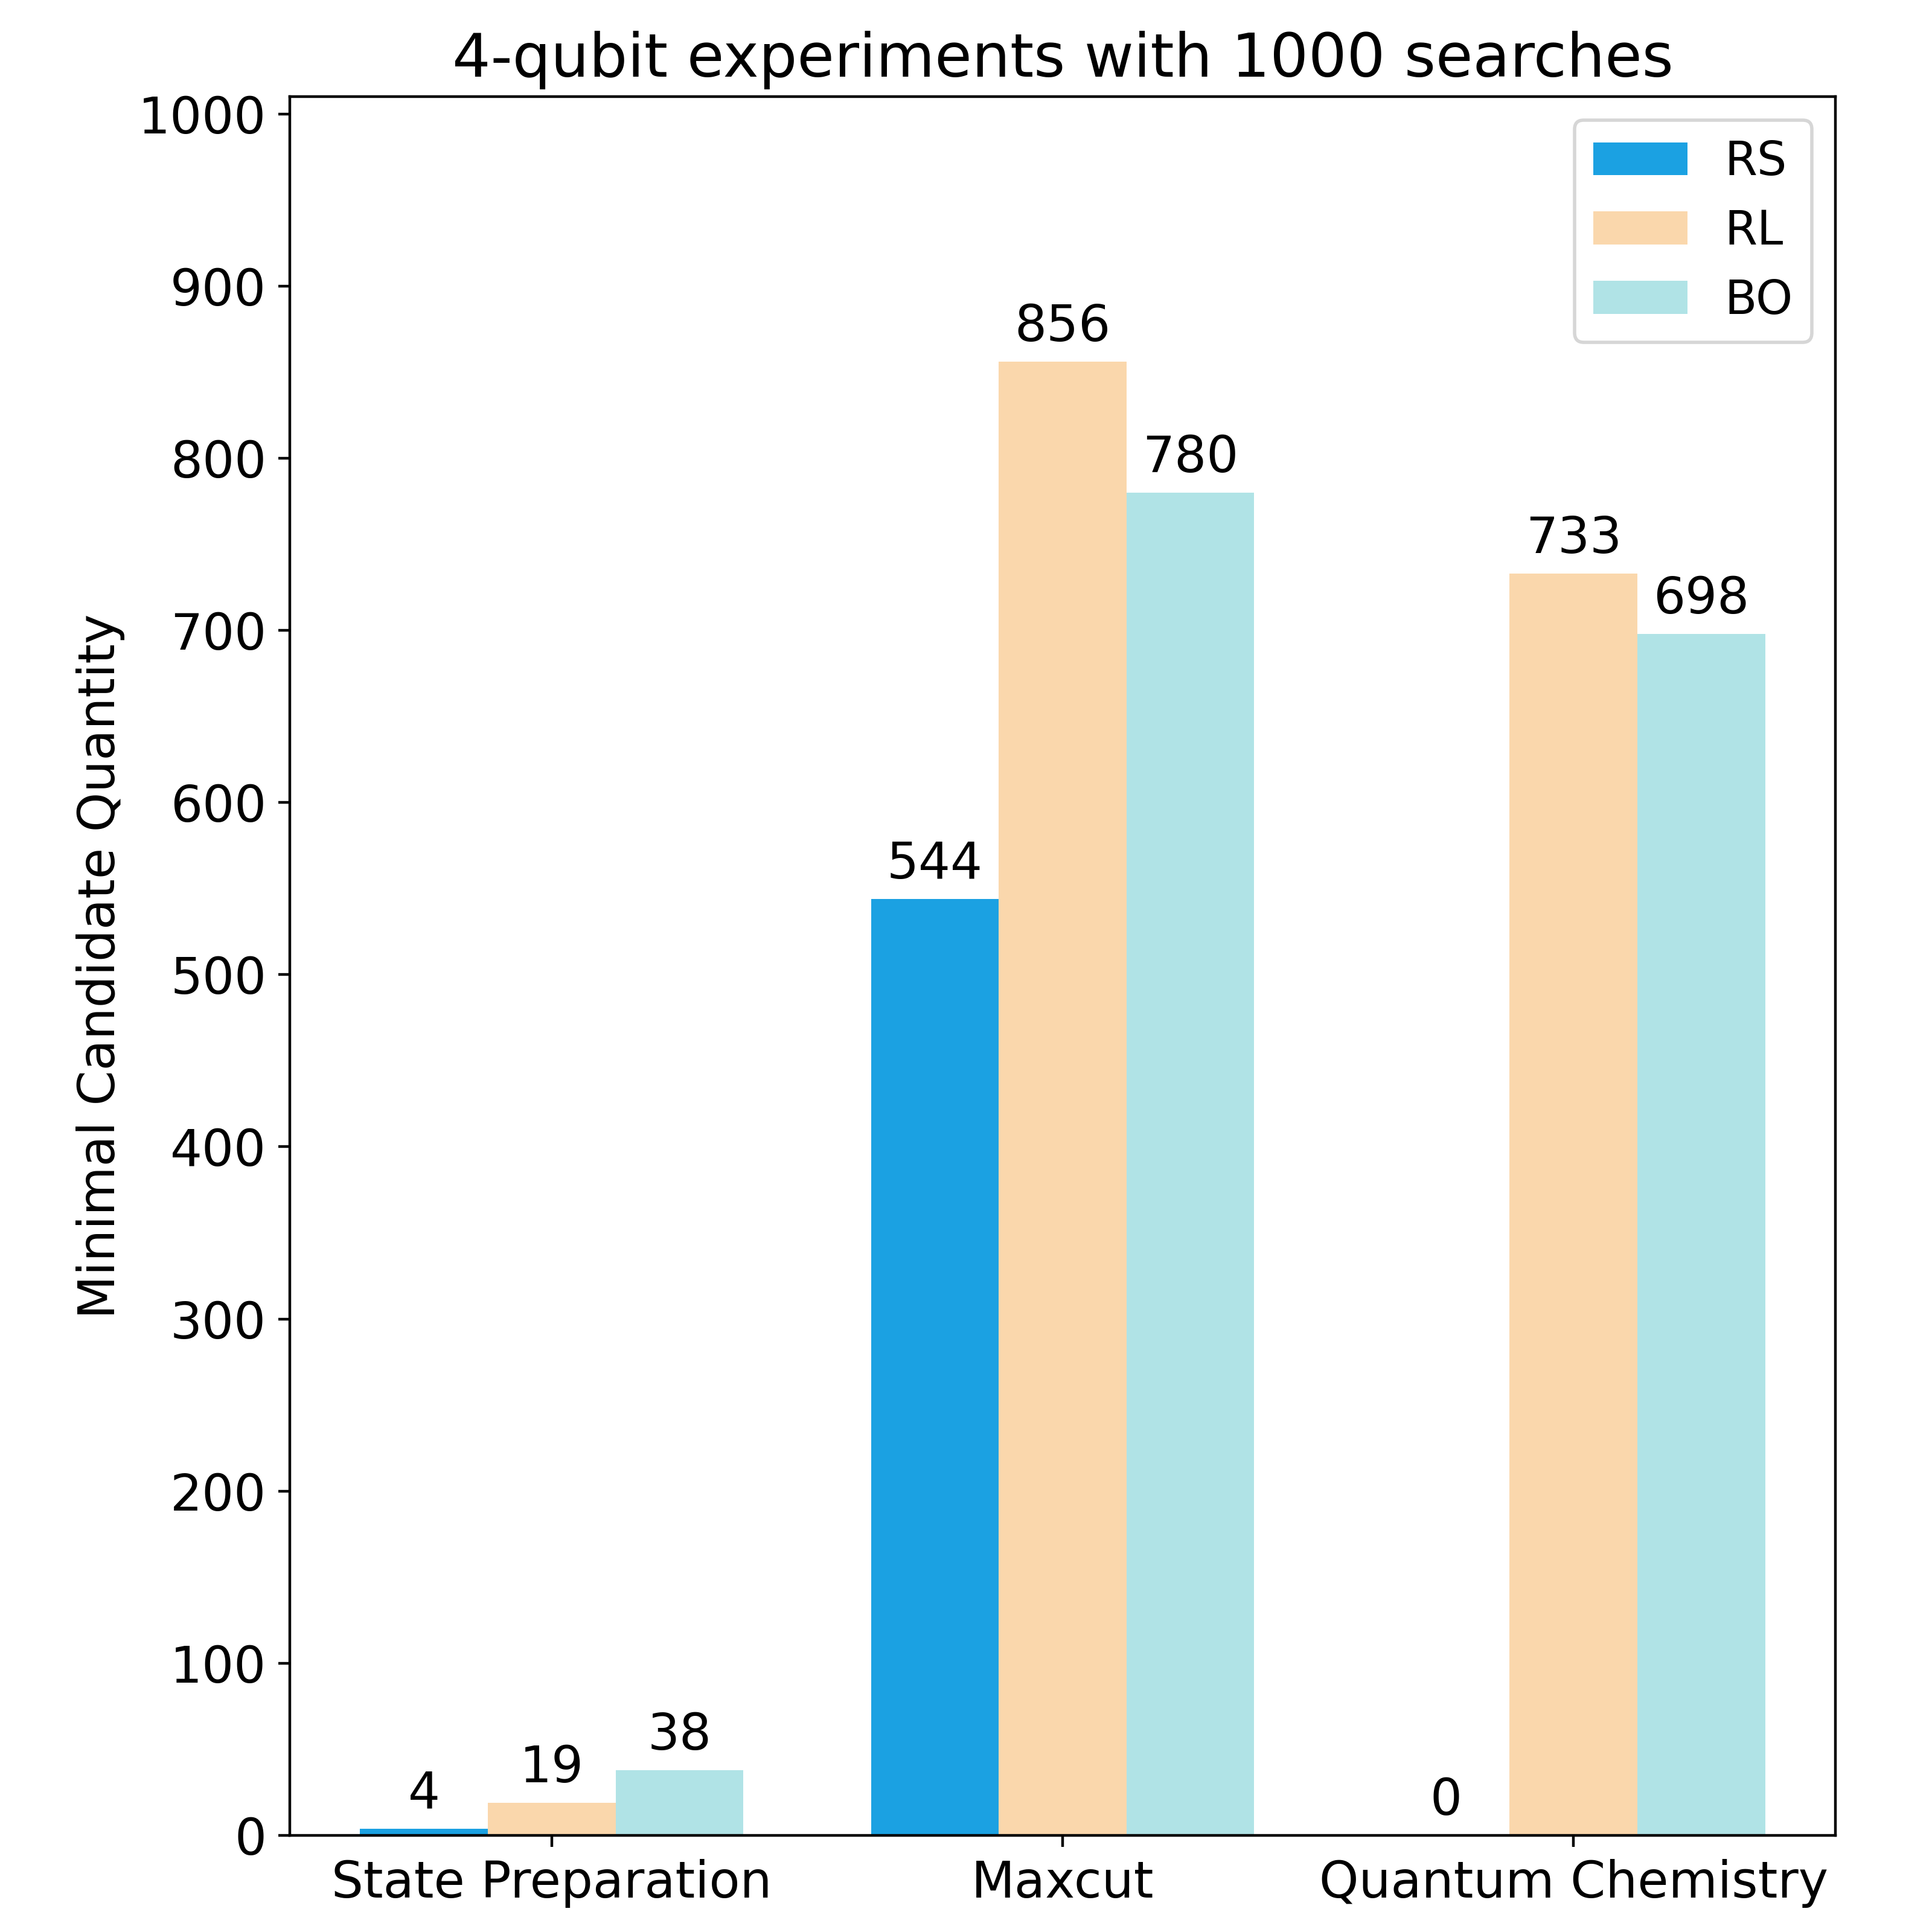
\includegraphics[width=\textwidth]{images/4-qubits_experiments_candidates_min.png}  % replace with actual inset image file path
        \end{minipage}
    \caption{4-qubit experiments}
    \label{4-qubits_candidates}
    \end{subfigure}
    \hspace{-1.5em}
    %\hfill
    \begin{subfigure}[b]{0.48\textwidth}
        \centering
        % Inset figures for (b)
        \begin{minipage}[b]{0.7\textwidth}
            \centering
            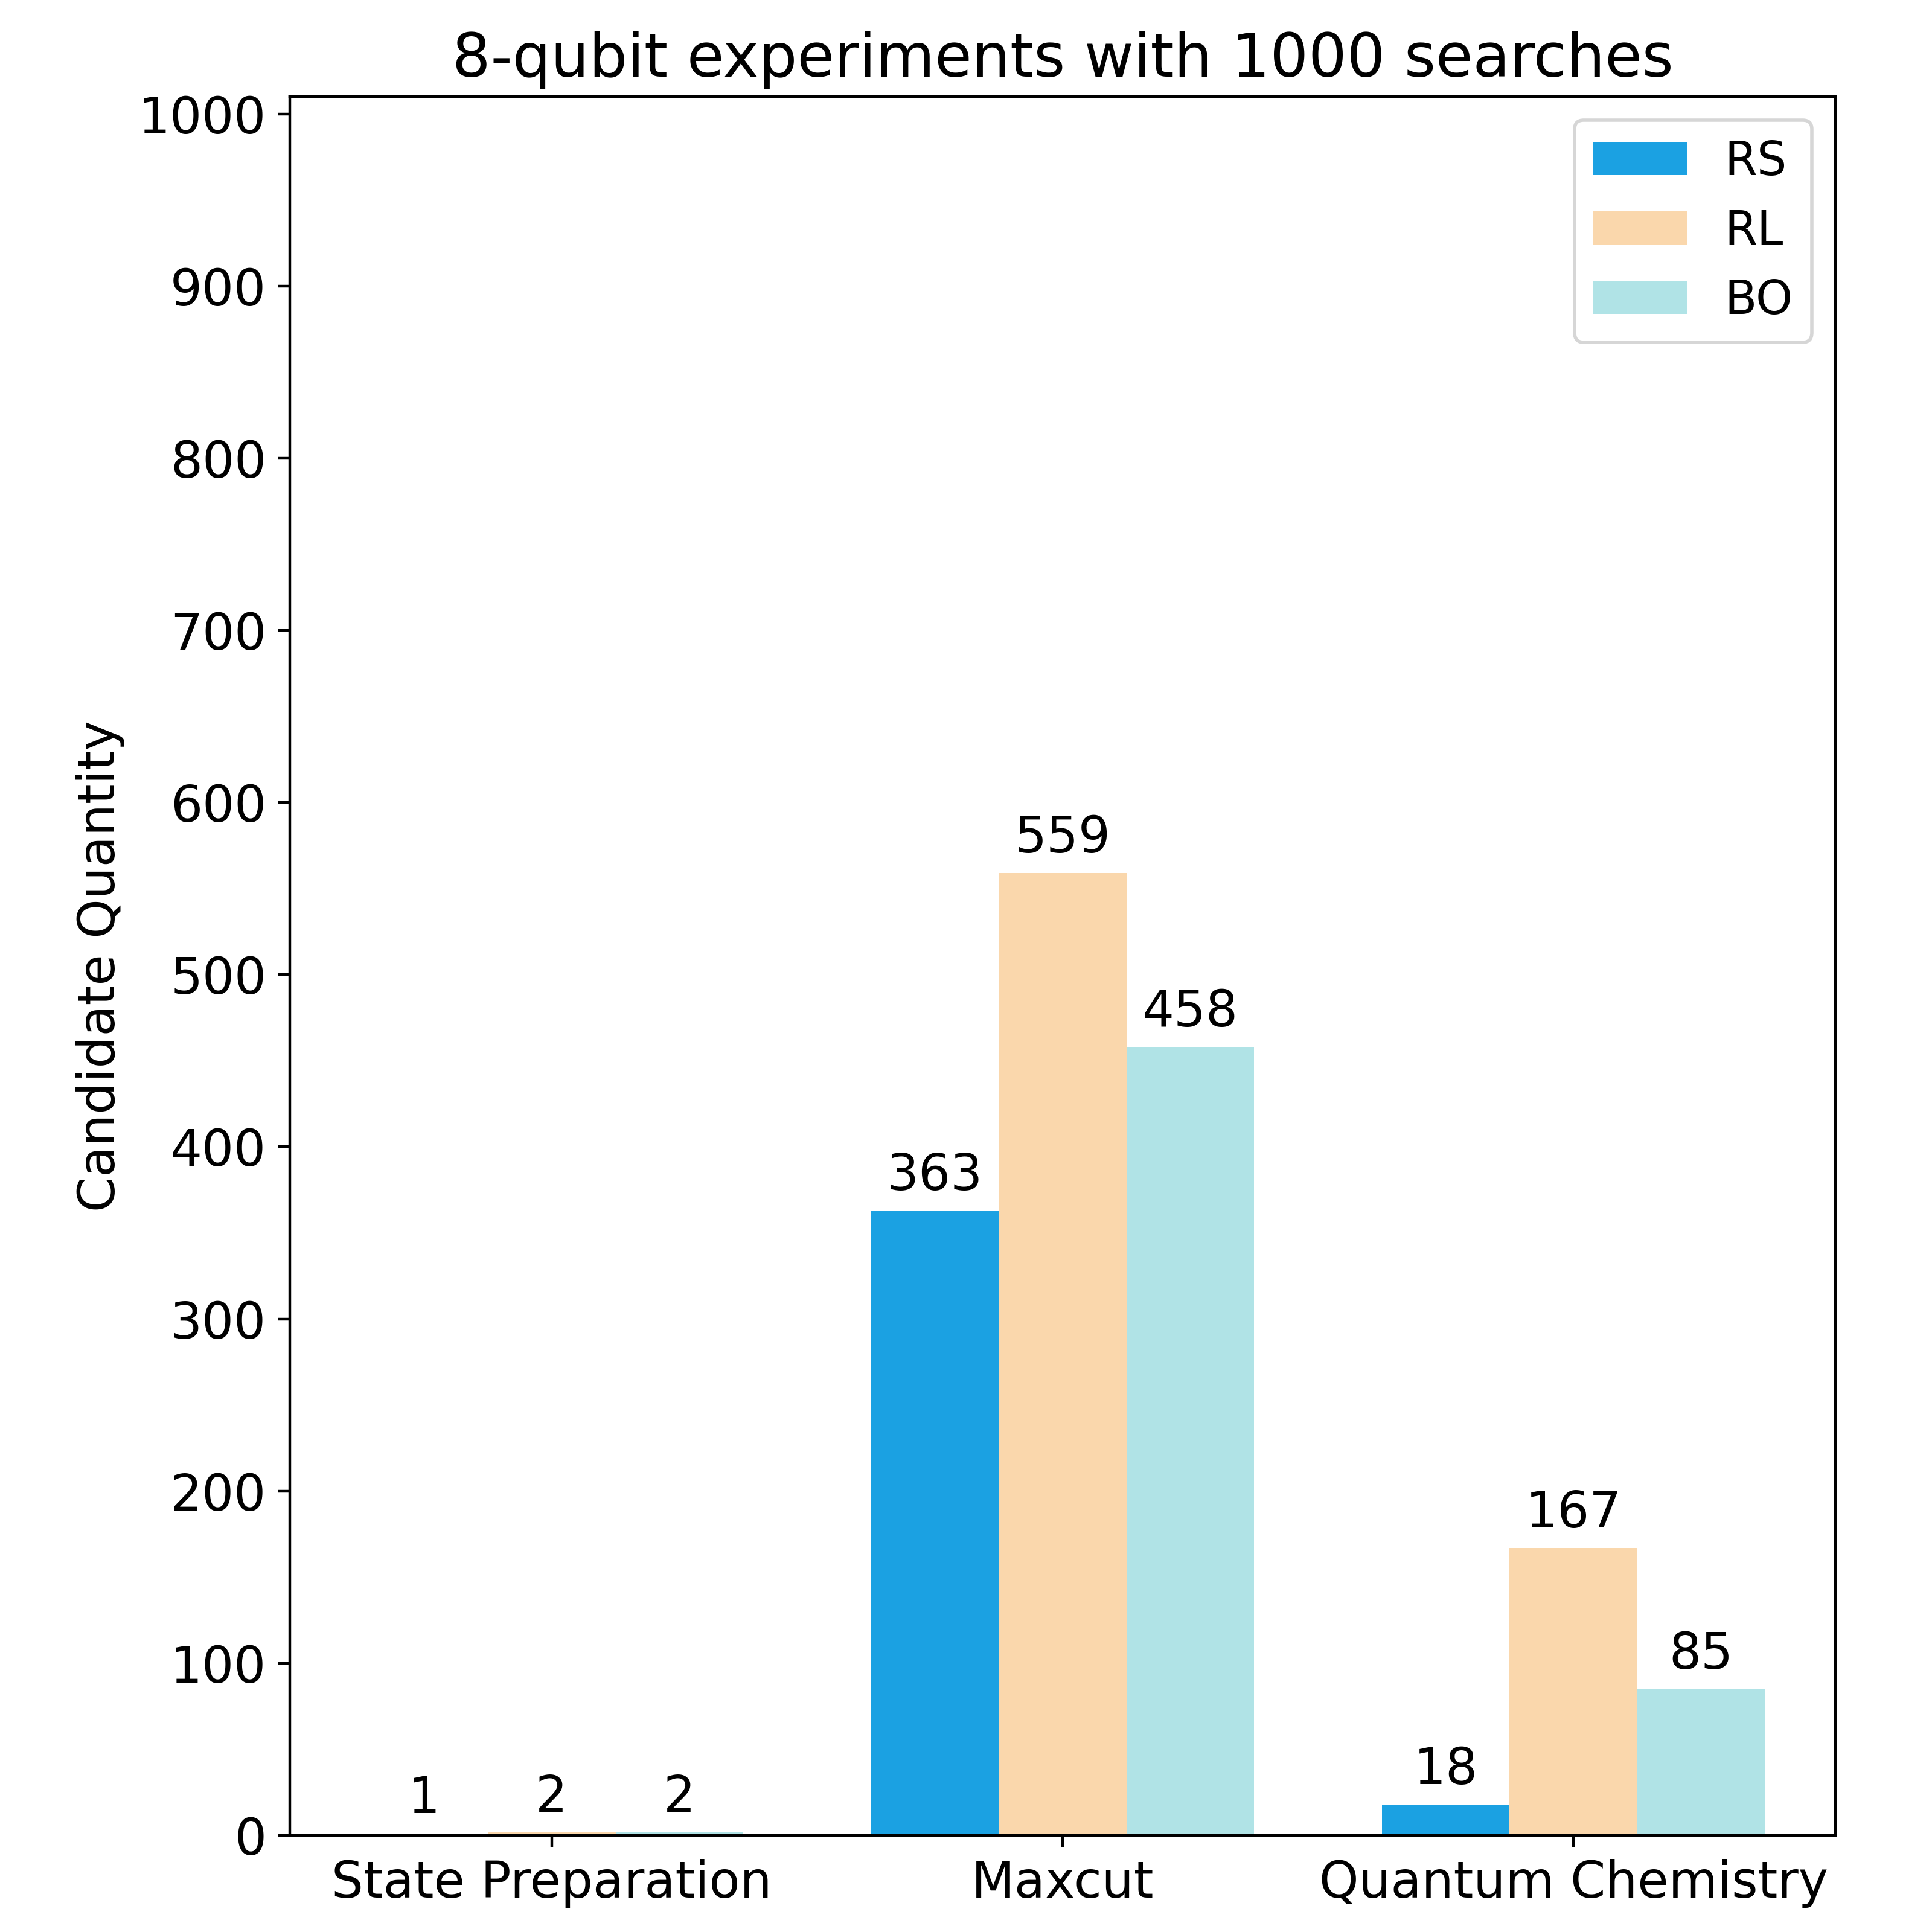
\includegraphics[width=0.8\textwidth]{images/8-qubits_experiments_candidates.png}
        \end{minipage}
        \hspace{-1em}
        \begin{minipage}[b]{0.28\textwidth}
            \centering
            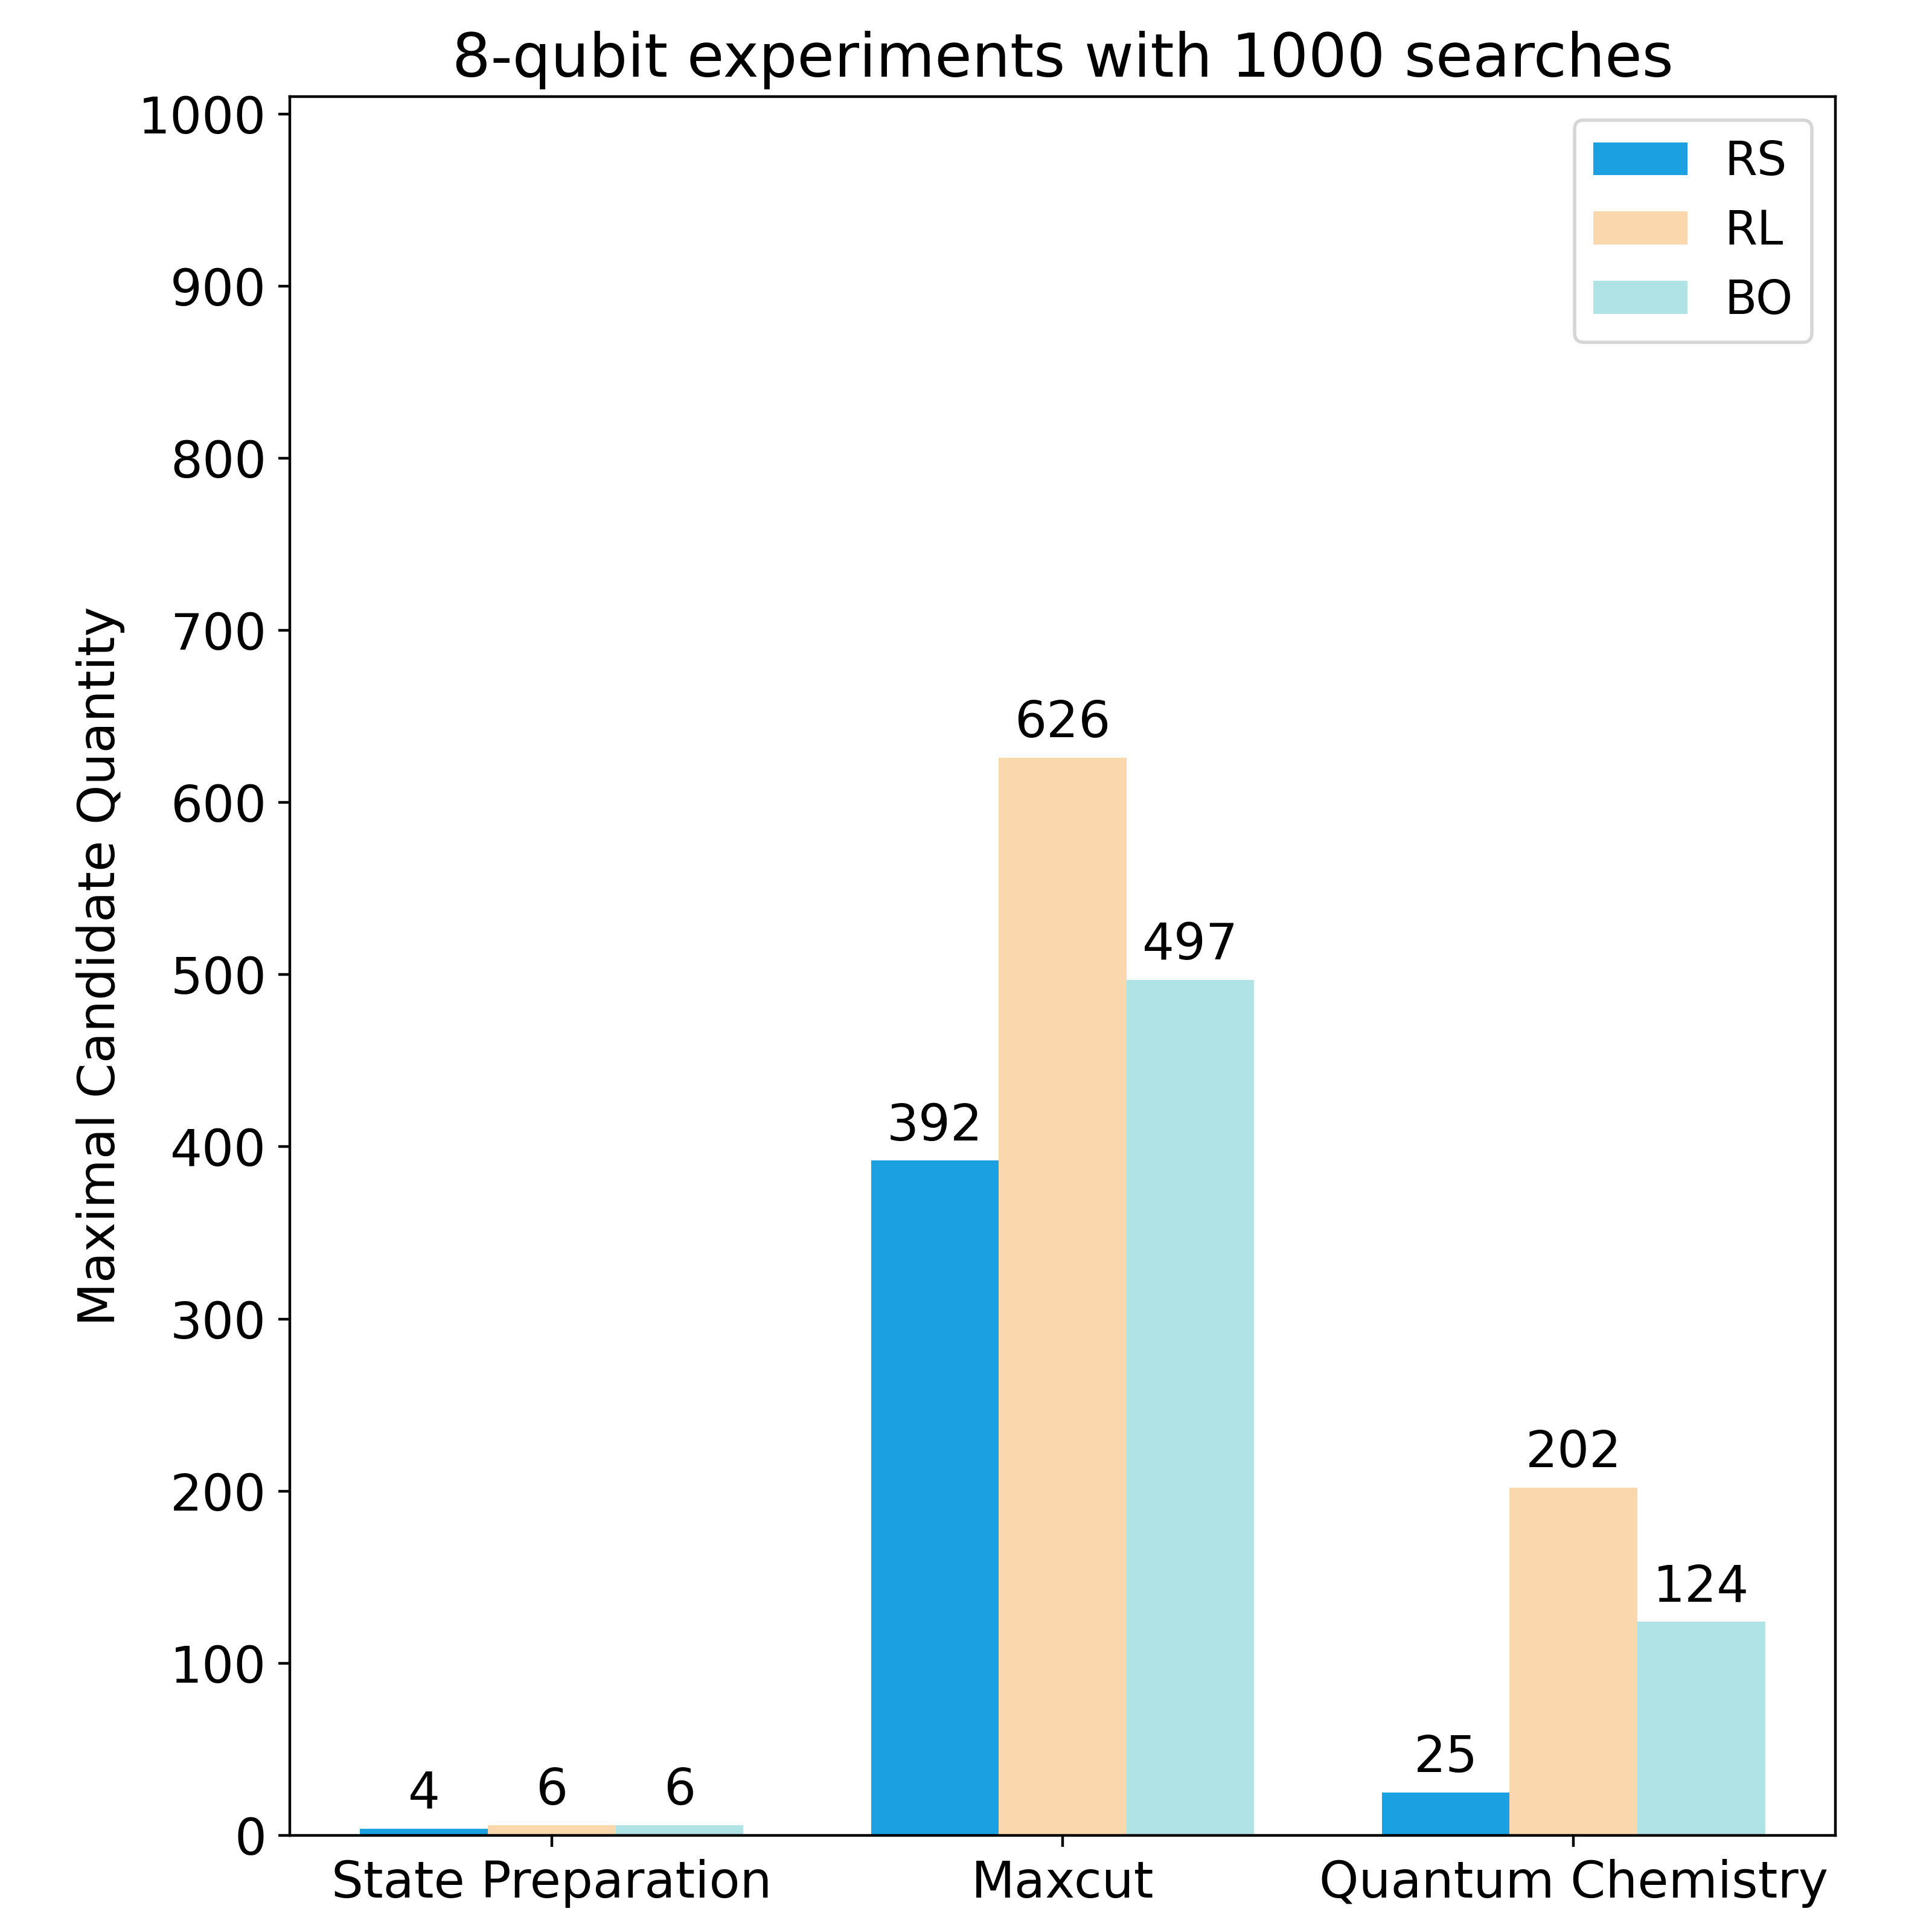
\includegraphics[width=\textwidth]{images/8-qubits_experiments_candidates_max.png}
            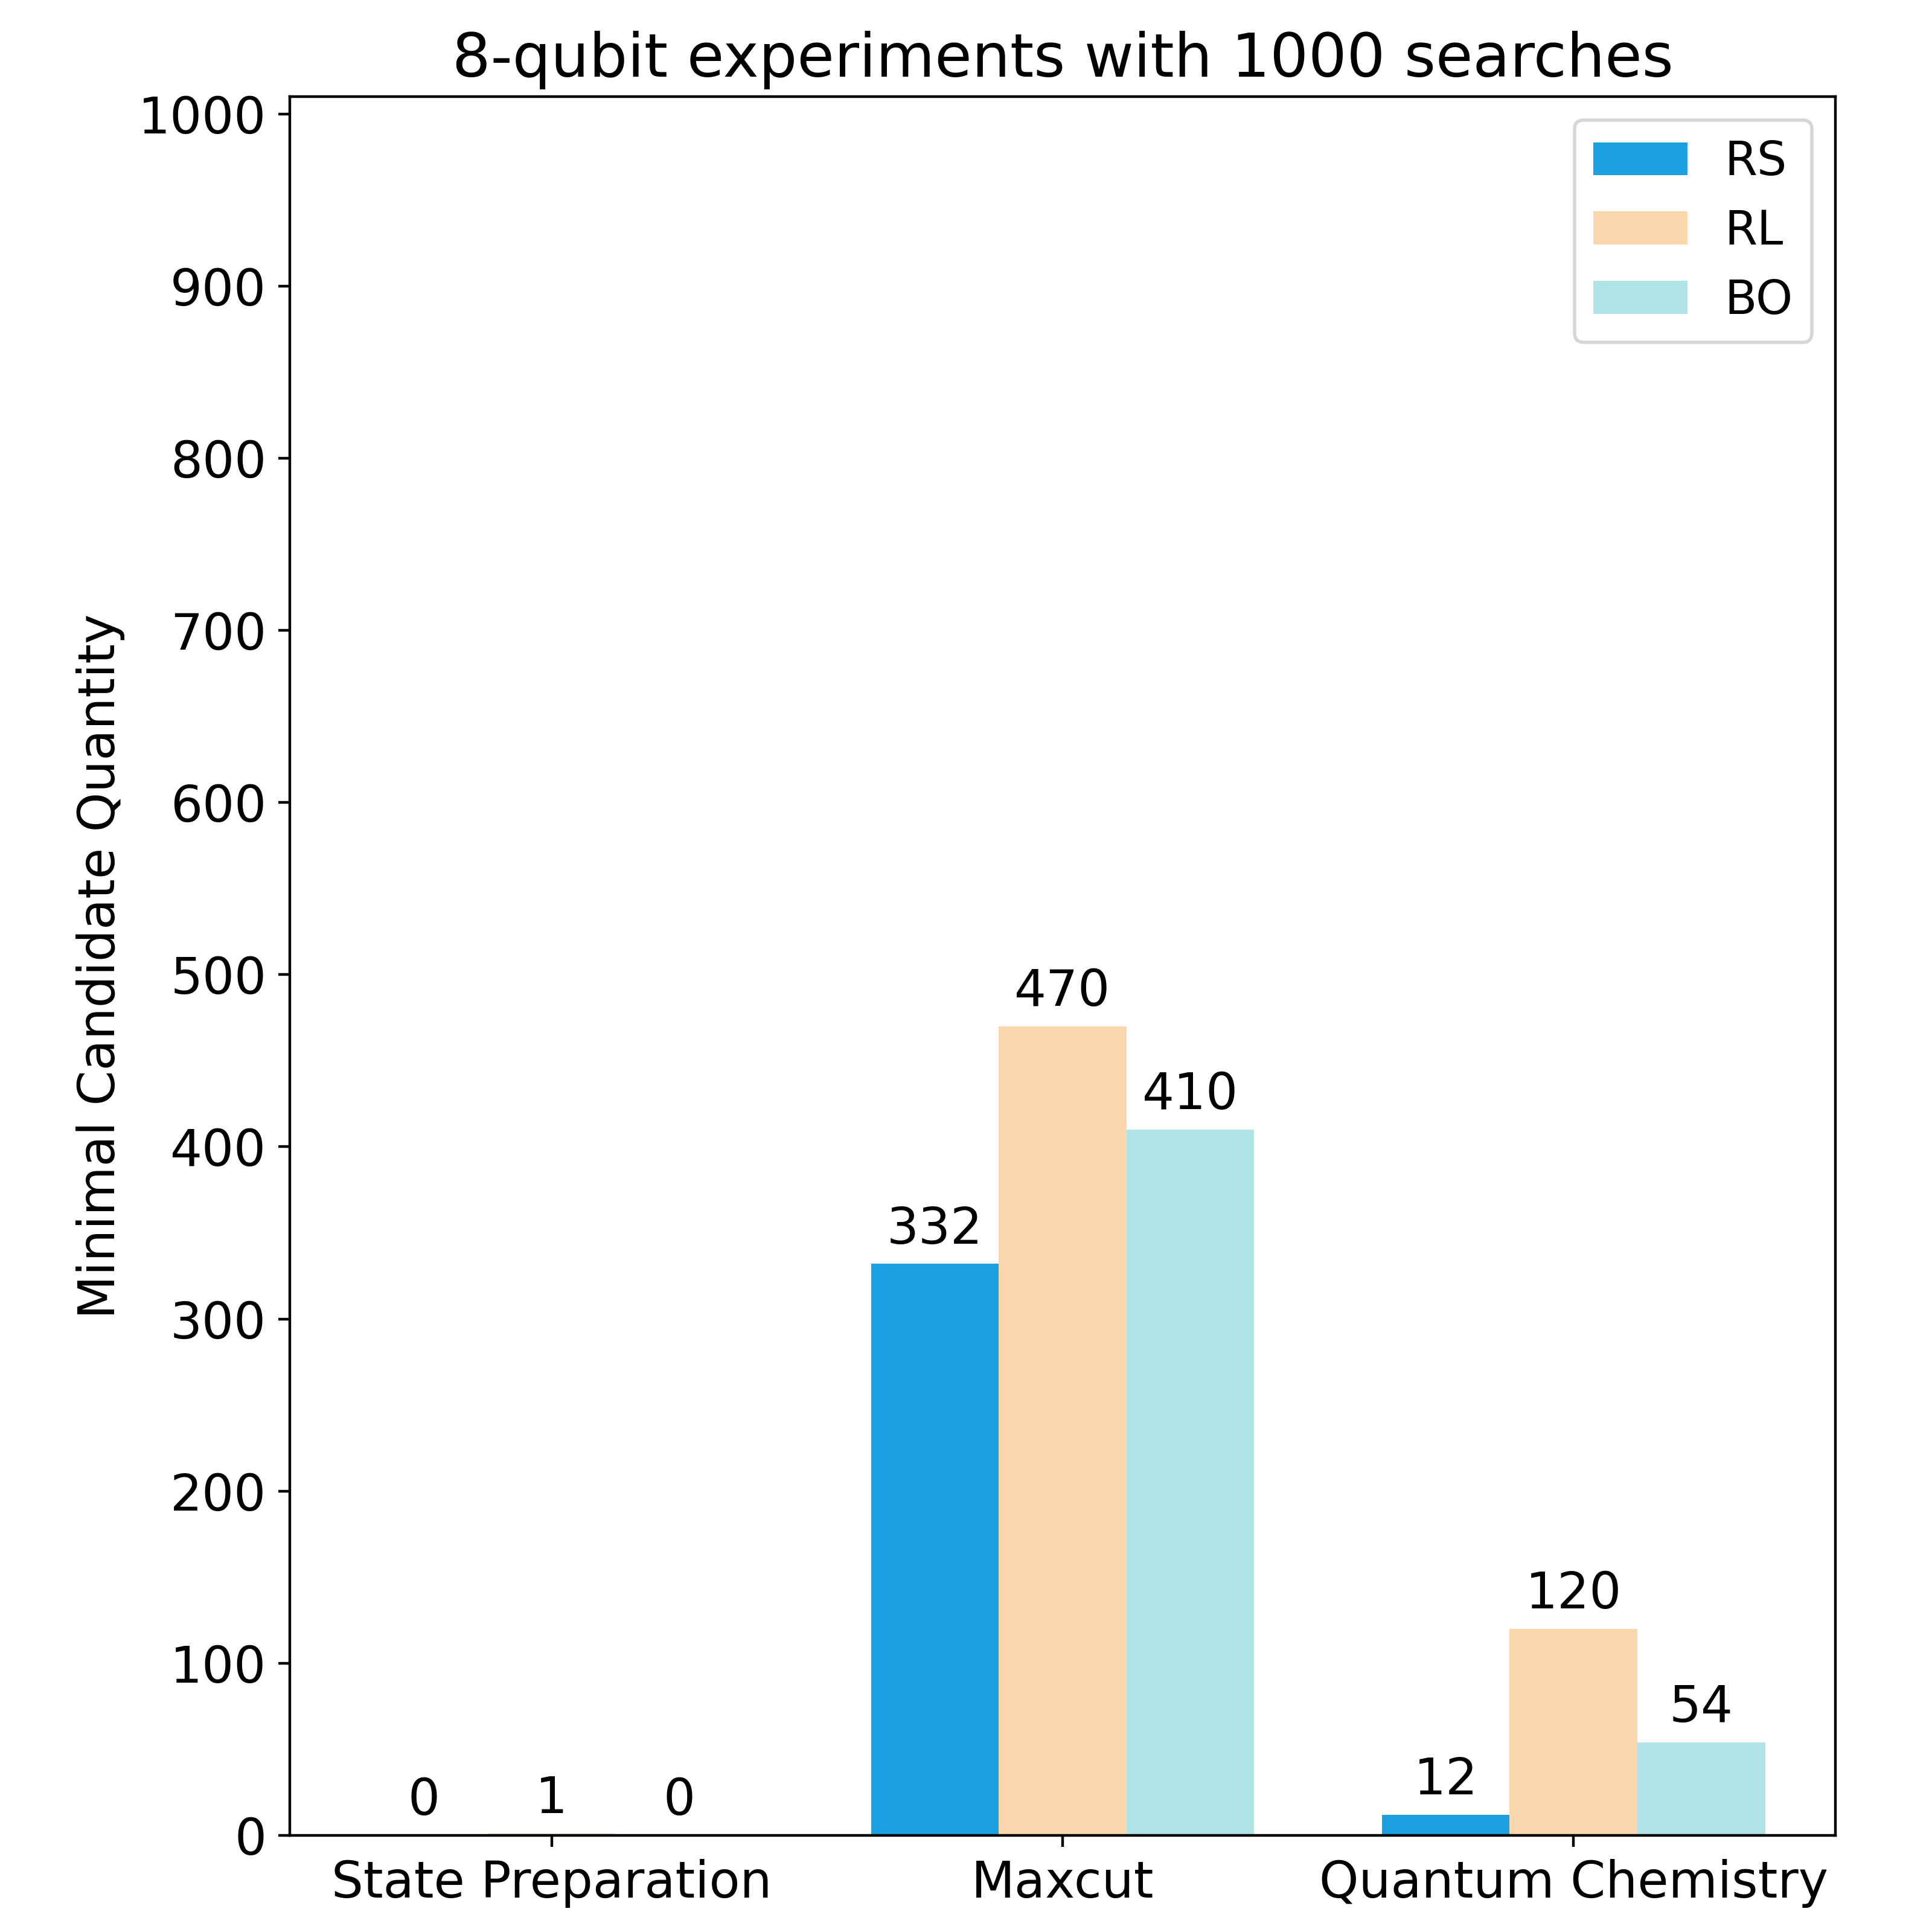
\includegraphics[width=\textwidth]{images/8-qubits_experiments_candidates_min.png}  % replace with actual inset image file path
        \end{minipage}
    \caption{8-qubit experiments}
    \label{8-qubits_candidates}
    \end{subfigure}
    \caption{The candidate quantities for the 4-qubit and 8-qubit applications. RS, RL, and BO refer to Random Search, REINFORCE, and Bayesian Optimization, respectively. The reward threshold for all 4-qubit experiments is 0.95, while for the more complex 8-qubit experiments, the thresholds are softer: 0.75 for state preparation, 0.925 for max-cut, and 0.95 for quantum chemistry. Each experiment is performed with 1000 queries, meaning only 1000 samples are drawn from a search space of 100,000 circuits. Additionally, the left-hand side of subfigures (a) and (b) shows the average results over 50 runs (with different random seeds), while the right-hand side shows the maximum and minimum candidate quantities across the 50 runs.}
    \label{candidates}
\end{figure}

% \begin{figure}[ht]
% \begin{center}
%     \begin{subfigure}[b]{0.4\textwidth}
%     \centering
%     \includegraphics[width=\textwidth]{images/4-qubits_experiments_candidates_combined.png} %
%     \caption{4-qubit experiments}
%     \label{4-qubits_candidates}
%     \end{subfigure}
%     \hspace{0.6cm}
%     \begin{subfigure}[b]{0.4\textwidth}
%     \centering
%     \includegraphics[width=\textwidth]{images/8-qubits_experiments_candidates_combined.png}
%     \caption{8-qubit experiments}
%     \label{8-qubits_candidates}
%     \end{subfigure}
%     \caption{Candidate quantity of 4-qubit and 8-qubit applications. The reward thresholds of all 4-qubit experiments are 0.95, but 8-qubit experiments are more complex, so their thresholds are soft. The thresholds of the 8-qubit state preparation, max-cut, and quantum chemistry experiments are 0.75, 0.925, and 0.9 respectively. All experiments are executed for only 1000 queries, i.e. only 1000 search samples are performed from the search space of 100,000 circuits. Additionally, the left results in (a) and (b) are the average of 50 runs (using different random seeds) and the right ones correspond to the maximal and minimum candidate quantity in the 50 runs.}
%     \label{candidates}   
% \end{center}
% \end{figure}

% \begin{table}[ht]
% \caption{Compare the QAS performance of different QAS methods for the 4-qubit state preparation.} % title name of the table
% \centering % centering table  
% \begin{tabular}{c c c cccccc} % creating 10 columns
% \hline\hline
% \addlinespace[0.5ex]
%  Method & $F_{thr}$ & $N_{lbl}$ & $N_{rest}$ & $N_{>0.95}$ & $N_{eval}$ & $N_{QAS}$ & $P_{opt}$ & $N_{QAS}/N_{eval}$
% \\ [0.5ex]  
% \hline
% \addlinespace[0.5ex]
% % Entering 1st row  
% \multirow{2}{*}{GNN$_{URL}$} & 0.4 & 1000 & 18963 & 2255 & 2000 & 120 & $\approx 1.00$ & 0.0600 \\[0.5ex] 
% &0.5 & 1000 & 5182 & 913 & 2000 & 183 & $\approx 1.00$ & 0.0915 \\[0.5ex]  
% % Entering 2nd row  
% \multirow{2}{*}{GSQAS$_{URL}$} & 0.4 & 1000 & 20876 & 2380 & 2000 & 116 & $\approx 1.00$ & 0.0580 \\[0.5ex]  
% & 0.5 & 1000 & 6228 & 1036 & 2000 & 168 & $\approx 1.00$ & 0.0840 \\[0.5ex]  
% % Entering 3rd row  
% DQAS & - & 0 & - & - & 1000 & 0 & $\approx 0.86$ & 0 \\[0.5ex]
% \hline
% \addlinespace[0.5ex]
% QAS$_{URL\&RL}$ & - & 0 & 100000 & \textbf{4729} & 1000 & 178 & $\approx \textbf{1.00}$ & \textbf{0.1780} \\[0.5ex]
% % [1ex] adds vertical space  
% \hline % inserts single-line  
% \end{tabular}
% \label{comparison1}
% \end{table}
\begin{table}[ht]
\centering % centering table
\scriptsize
\begin{tabular}{l | l l l lllll} % creating 10 columns
\hline\hline
\addlinespace[0.5ex]
 Method & $Task$ & $F_{thr}$ & $N_{lbl}$ & $N_{rest}$ & $N_{>0.95}$ & $N_{eval}$ & $N_{QAS}$ & $N_{QAS}/N_{eval}$
\\ [0.5ex]  
\hline
\addlinespace[0.5ex]
% Entering 1st row  
\multirow{3}{*}{GNN$^{URL}$} & \text{Fidelity} & 0.5 & 1000 & 21683 & 780 & 2000 & 36 & 0.0180 \\[0.5ex] 
& \text{Max-Cut} & 0.9 & 1000 & 45960 & 35967 & 2000 & 783 & 0.3915 \\[0.5ex]
& \text{QC-4}$_{H_2}$ & 0.8 & 1000 & 65598 & 18476 & 2000 & 278 & 0.1390 \\[0.5ex]
% Entering 2nd row  
\multirow{3}{*}{GSQAS$^{URL}$} & \text{Fidelity} & 0.5 & 1000 & 21014 & 768 & 2000 & 37 & 0.0185 \\[0.5ex]
& \text{Max-Cut} & 0.9 & 1000 & 43027 & 33686 & 2000 & 785 & 0.3925 \\[0.5ex]
& \text{QC-4}$_{H_2}$ & 0.8 & 1000 & 30269 & 19889 & 2000 & 658 & 0.3290 \\[0.5ex]
% \multirow{3}{*}{QAS$^{URL}_{Random}$} & \text{Fidelity} & - & 0 & 100000 & \textbf{1606} & 1000 & 15 & 0.0150 \\[0.5ex]
% & \text{Max-Cut} & - & 0 & 100000 & \textbf{57116} & 1000 & 568 & 0.5680 \\[0.5ex]
% & \text{QC}$_{H}$ & - & 0 & 100000 & \textbf{37799} & 1000 & 371 & 0.3710\\[0.5ex]
% \multirow{3}{*}{QAS$^{URL}_{OtherEncoding}$} & \text{Fidelity} & - & 0 & 100000 & \textbf{4729} & 1000 & \textbf{178} & \textbf{0.1780} \\[0.5ex]
% & \text{Max-Cut} & - & 0 & 100000 & 37709 & 1000 & 727 & 0.7270 \\[0.5ex]
% & \text{QC}$_{H}$ & - & 0 & 100000 & 22514 & 1000 & 531 & 0.5310 \\[0.5ex]
% Entering 3rd row  
%DQAS & - & 0 & - & - & 1000 & 0 & $\approx 0.86$ & 0 \\[0.5ex]
\multirow{3}{*}{Random Search} 
& \text{Fidelity} & - & 0 & 100000 & 1606 & 1000 & 15 & 0.0150 \\[0.5ex]
& \text{Max-Cut} & - & 0 & 100000 & 57116 & 1000 & 568 & 0.5680 \\[0.5ex]
& \text{QC-4}$_{H_2}$ & - & 0 & 100000 & 37799 & 1000 & 371 & 0.3710 \\[0.5ex]
\hline
\addlinespace[0.5ex]
\multirow{3}{*}{QAS$^{URL}_{RL(BO)}$} & \text{Fidelity} & - & 0 & 100000 & \textbf{1606} & \textbf{1000} & \textbf{69}(63) & \textbf{0.0690}(0.0630) \\[0.5ex]
& \text{Max-Cut} & - & 0 & 100000 & \textbf{57116} & \textbf{1000} & \textbf{898}(820) & \textbf{0.8980}(0.8200) \\[0.5ex]
& \text{QC-4}$_{H_2}$ & - & 0 & 100000 & \textbf{37799} & \textbf{1000} & \textbf{817}(739) & \textbf{0.8170}(0.7390) \\[0.5ex]
% \multirow{3}{*}{QAS$_{URL\&BO}$} & \text{Fidelity} & 0.95 & 100000 & 1606 & 768 & 2000 & 63 & 0.0315 \\[0.5ex] 
% & \text{Max-Cut} & 0.95 & 100000 & 57116 & 33686 & 2000 & 820 & 0.41 \\[0.5ex]
% & \text{QC}$_{H}$ & 0.95 & 100000 & 37799 & 16855 & 2000 & 739 & 0.3695 \\[0.5ex] 
% [1ex] adds vertical space  
\hline % inserts single-line 
\end{tabular}
\caption{Compare the QAS performance of different QAS methods for the 4-qubit tasks. URL denotes unsupervised representation learning, $F_{thr}$ is the threshold to filter poor-performance architectures, $N_{lbl}$, $N_{rest}$ and $N_{>0.95}$ refer to the number of required labeled circuits, rest circuits after filtering and the circuits that achieve the performance higher than 0.95 in the rest circuits respectively. $N_{eval}$ represents the number of evaluated circuits, i.e. the sum of the number of labeled and sampled circuits, $N_{QAS}$ is the number of searched candidates in average of 50 runs.}
% , and $P_{opt}$ represents the achieved optimal performance (reward in the range $[0, 1]$).} % title name of the table
\label{comparison1}
\end{table}

\begin{table}[ht]
\centering % centering table
\scriptsize  % Change to \tiny, \scriptsize, \footnotesize, \small, \normalsize, \large, \Large, \LARGE, or \huge as needed
\begin{tabular}{l | l llll}
\hline\hline
\addlinespace[0.5ex]
 Method & Encoding $\mathcal{E}$ & $N_{rest}$ & $N_{eval}$ & $N_{QAS}$ & $N_{QAS}/N_{eval}$
\\ [0.5ex]  
\hline
\addlinespace[0.5ex]
% Entering 1st row  
\multirow{2}{*}{GSQAS$_{4}$}
& \text{GSQAS} & 25996 & 2000 & 625 & 0.3125 \\[0.5ex]
& \text{Ours} & 30269 & 2000 & \textbf{658} & \textbf{0.3290} \\[0.5ex]
\hline
\addlinespace[0.5ex]
\multirow{2}{*}{GSQAS$_{12}$}
& \text{GSQAS} & 60088 & 2000 & \textbf{283} & \textbf{0.1415} \\[0.5ex]
& \text{Ours} & 60565 & 2000 & 276 & 0.1380 \\[0.5ex]
\hline
\addlinespace[0.5ex]
\multirow{2}{*}{QAS$_{RL-4}$} 
& \text{GSQAS} & 100000 & 1000 & 760 & 0.7600 \\[0.5ex]
& \text{Ours} & 100000 & 1000 & \textbf{817} & \textbf{0.8170} \\[0.5ex]
% \hline
% \addlinespace[0.5ex]
% \multirow{2}{*}{QAS$_{RL-6}$} 
% & \text{GSQAS} & 100000 & 1000 & 97 & 0.0970 \\[0.5ex]
% & \text{URL} & 100000 & 1000 & 54 & 0.0540 \\[0.5ex]
\hline
\addlinespace[0.5ex]
\multirow{2}{*}{QAS$_{RL-8}$} 
& \text{GSQAS} & 100000 & 1000 & 160 & 0.1600 \\[0.5ex]
& \text{Ours} & 100000 & 1000 & \textbf{167} & \textbf{0.1670} \\[0.5ex]
\hline
\addlinespace[0.5ex]
\multirow{2}{*}{QAS$_{RL-12}$} 
& \text{GSQAS} & 100000 & 1000 & \textbf{422} & \textbf{0.4220} \\[0.5ex]
& \text{Ours} & 100000 & 1000 & 392 & 0.3920\\[0.5ex]
\hline
\addlinespace[0.5ex]

% [1ex] adds vertical space  
\hline % inserts single-line 
\end{tabular}
\caption{We compare the QAS performance of different encodings using various search methods. For the 4- and 12-qubit quantum chemistry tasks, we select $H_2$ and $LiH$, respectively, while for the 8-qubit task, we use the TFIM. The results represent the average of 50 runs.}
% , and $P_{opt}$ represents the achieved optimal performance (reward in the range $[0, 1]$).} % title name of the table
\label{comparison-2}
\end{table}

\textbf{Observation (3):} In Table \ref{comparison1}, we compare various QAS methods with our approach on the 4-qubit state preparation task, using a circuit space of 100,000 circuits and limiting the search to 1000 queries. GNN$^{URL}$ and GSQAS$^{URL}$ represent predictor-based methods from \citet{he2023gnn} and \citet{he2023gsqas}, respectively, both employing our pre-trained model. QAS$^{URL}_{RL(BO)}$ denotes the QAS approach with REINFORCE (BO) used in this work. The average results over 50 runs indicate that both the predictor-based methods and our approach are capable of identifying a significant number of high-performance circuits with fewer samples.
However, predictor-based methods rely on labeled circuits to train predictors, introducing uncertainty as they may inadvertently filter out well-performing architectures along with poor ones. While a higher $F_{thr}$ value filters out more low-performance circuits, increasing the proportion of good architectures in the filtered space, it also sacrifices many well-performing circuits, which can lead to improved Random Search performance but at the cost of excluding some optimal circuits.
Despite these trade-offs, our method achieves comparable performance to predictor-based methods, demonstrating higher efficiency in terms of $N_{QAS}/N_{eval}$ while requiring fewer circuit evaluations.
In Appendix \ref{Best candidate circuits}, we present the best candidate circuits acquired by each of the three methods for every experiment.

\textbf{Observation (4):} In Table \ref{comparison-2}, we present the search performance across different frameworks and encoding methods, focusing on 4-, 8-, and 12-qubit quantum chemistry tasks for comparison. In most cases, our encoding method achieves the highest search efficiency, although the performance for the 12-qubit task is slightly lower than with another encoding method. Combined with the representation learning results in Figure \ref{2D-Visu}, we observe that the search is significantly more efficient when the learned circuit representation is smooth and concentrated. For the 12-qubit experiments, the circuits used for representation learning may be insufficient to fully capture the search space, leading to representation learning failures, as shown in Figure \ref{fig:PCA-12}, and resulting in a decline in search efficiency.

% \textbf{Observation (4):} In Appendix \ref{Best candidate circuits}, we present the best candidate circuits acquired by each of the three methods for every experiment. These circuits exhibit a higher likelihood of being discovered by REINFORCE and BO in contrast to Random Search. This observation underscores the superior search capabilities of REINFORCE and BO in navigating the large and diverse search space generated by our approach, which is based on a random generator derived from a fixed operation pool. Unlike conventional approaches that adhere to layer-wise circuit design baselines, our method excels in discovering circuits with fewer trainable parameters. This characteristic is of paramount importance when addressing real-world optimization challenges in QAS. In conclusion, our approach not only enhances the efficiency of candidate circuit discovery but also accommodates the distinct characteristics of various problem domains through a large and diverse search space.

\section{Conclusion}
Inspired by the \textit{Arch2vec} method \citep{yan2020does}, we focus on exploring whether unsupervised architecture representation learning can enhance QAS. By decoupling unsupervised architecture representation learning from the QAS process, we successfully eliminate the need for a large number of labeled circuits. Additionally, our proposed quantum circuit encoding scheme addresses limitations in existing representations, improving search performance through more accurate and effective embeddings. Furthermore, our framework conducts QAS without relying on a predictor by directly applying search algorithms, such as REINFORCE and Bayesian Optimization (BO), to the latent representations. We have demonstrated the effectiveness of this approach through various experiments. In our framework, the success of QAS depends on the quality of unsupervised architecture representation learning and the selection of search algorithms. Thus, we recommend further investigation into architecture representation learning for QAS, as well as the development of more efficient search strategies within the latent representation space.

% \section{Submission of conference papers to ICLR 2024}

% ICLR requires electronic submissions, processed by
% \url{https://openreview.net/}. See ICLR's website for more instructions.

% If your paper is ultimately accepted, the statement {\tt
%   {\textbackslash}iclrfinalcopy} should be inserted to adjust the
% format to the camera ready requirements.

% The format for the submissions is a variant of the NeurIPS format.
% Please read carefully the instructions below, and follow them
% faithfully.

% \subsection{Style}

% Papers to be submitted to ICLR 2024 must be prepared according to the
% instructions presented here.

% %% Please note that we have introduced automatic line number generation
% %% into the style file for \LaTeXe. This is to help reviewers
% %% refer to specific lines of the paper when they make their comments. Please do
% %% NOT refer to these line numbers in your paper as they will be removed from the
% %% style file for the final version of accepted papers.

% Authors are required to use the ICLR \LaTeX{} style files obtainable at the
% ICLR website. Please make sure you use the current files and
% not previous versions. Tweaking the style files may be grounds for rejection.

% \subsection{Retrieval of style files}

% The style files for ICLR and other conference information are available online at:
% \begin{center}
%    \url{http://www.iclr.cc/}
% \end{center}
% The file \verb+iclr2024_conference.pdf+ contains these
% instructions and illustrates the
% various formatting requirements your ICLR paper must satisfy.
% Submissions must be made using \LaTeX{} and the style files
% \verb+iclr2024_conference.sty+ and \verb+iclr2024_conference.bst+ (to be used with \LaTeX{}2e). The file
% \verb+iclr2024_conference.tex+ may be used as a ``shell'' for writing your paper. All you
% have to do is replace the author, title, abstract, and text of the paper with
% your own.

% The formatting instructions contained in these style files are summarized in
% sections \ref{gen_inst}, \ref{headings}, and \ref{others} below.

% \section{General formatting instructions}
% \label{gen_inst}

% The text must be confined within a rectangle 5.5~inches (33~picas) wide and
% 9~inches (54~picas) long. The left margin is 1.5~inch (9~picas).
% Use 10~point type with a vertical spacing of 11~points. Times New Roman is the
% preferred typeface throughout. Paragraphs are separated by 1/2~line space,
% with no indentation.

% Paper title is 17~point, in small caps and left-aligned.
% All pages should start at 1~inch (6~picas) from the top of the page.

% Authors' names are
% set in boldface, and each name is placed above its corresponding
% address. The lead author's name is to be listed first, and
% the co-authors' names are set to follow. Authors sharing the
% same address can be on the same line.

% Please pay special attention to the instructions in section \ref{others}
% regarding figures, tables, acknowledgments, and references.


% There will be a strict upper limit of 9 pages for the main text of the initial submission, with unlimited additional pages for citations. 

% \section{Headings: first level}
% \label{headings}

% First level headings are in small caps,
% flush left and in point size 12. One line space before the first level
% heading and 1/2~line space after the first level heading.

% \subsection{Headings: second level}

% Second level headings are in small caps,
% flush left and in point size 10. One line space before the second level
% heading and 1/2~line space after the second level heading.

% \subsubsection{Headings: third level}

% Third level headings are in small caps,
% flush left and in point size 10. One line space before the third level
% heading and 1/2~line space after the third level heading.

% \section{Citations, figures, tables, references}
% \label{others}

% These instructions apply to everyone, regardless of the formatter being used.

% \subsection{Citations within the text}

% Citations within the text should be based on the \texttt{natbib} package
% and include the authors' last names and year (with the ``et~al.'' construct
% for more than two authors). When the authors or the publication are
% included in the sentence, the citation should not be in parenthesis using \verb|\citet{}| (as
% in ``See \citet{Hinton06} for more information.''). Otherwise, the citation
% should be in parenthesis using \verb|\citep{}| (as in ``Deep learning shows promise to make progress
% towards AI~\citep{Bengio+chapter2007}.'').

% The corresponding references are to be listed in alphabetical order of
% authors, in the \textsc{References} section. As to the format of the
% references themselves, any style is acceptable as long as it is used
% consistently.

% \subsection{Footnotes}

% Indicate footnotes with a number\footnote{Sample of the first footnote} in the
% text. Place the footnotes at the bottom of the page on which they appear.
% Precede the footnote with a horizontal rule of 2~inches
% (12~picas).\footnote{Sample of the second footnote}

% \subsection{Figures}

% All artwork must be neat, clean, and legible. Lines should be dark
% enough for purposes of reproduction; art work should not be
% hand-drawn. The figure number and caption always appear after the
% figure. Place one line space before the figure caption, and one line
% space after the figure. The figure caption is lower case (except for
% first word and proper nouns); figures are numbered consecutively.

% Make sure the figure caption does not get separated from the figure.
% Leave sufficient space to avoid splitting the figure and figure caption.

% You may use color figures.
% However, it is best for the
% figure captions and the paper body to make sense if the paper is printed
% either in black/white or in color.
% \begin{figure}[h]
% \begin{center}
% %\framebox[4.0in]{$\;$}
% \fbox{\rule[-.5cm]{0cm}{4cm} \rule[-.5cm]{4cm}{0cm}}
% \end{center}
% \caption{Sample figure caption.}
% \end{figure}

% \subsection{Tables}

% All tables must be centered, neat, clean and legible. Do not use hand-drawn
% tables. The table number and title always appear before the table. See
% Table~\ref{sample-table}.

% Place one line space before the table title, one line space after the table
% title, and one line space after the table. The table title must be lower case
% (except for first word and proper nouns); tables are numbered consecutively.

% \begin{table}[t]
% \caption{Sample table title}
% \label{sample-table}
% \begin{center}
% \begin{tabular}{ll}
% \multicolumn{1}{c}{\bf PART}  &\multicolumn{1}{c}{\bf DESCRIPTION}
% \\ \hline \\
% Dendrite         &Input terminal \\
% Axon             &Output terminal \\
% Soma             &Cell body (contains cell nucleus) \\
% \end{tabular}
% \end{center}
% \end{table}

% \section{Default Notation}

% In an attempt to encourage standardized notation, we have included the
% notation file from the textbook, \textit{Deep Learning}
% \cite{goodfellow2016deep} available at
% \url{https://github.com/goodfeli/dlbook_notation/}.  Use of this style
% is not required and can be disabled by commenting out
% \texttt{math\_commands.tex}.


% \centerline{\bf Numbers and Arrays}
% \bgroup
% \def\arraystretch{1.5}
% \begin{tabular}{p{1in}p{3.25in}}
% $\displaystyle a$ & A scalar (integer or real)\\
% $\displaystyle \va$ & A vector\\
% $\displaystyle \mA$ & A matrix\\
% $\displaystyle \tA$ & A tensor\\
% $\displaystyle \mI_n$ & Identity matrix with $n$ rows and $n$ columns\\
% $\displaystyle \mI$ & Identity matrix with dimensionality implied by context\\
% $\displaystyle \ve^{(i)}$ & Standard basis vector $[0,\dots,0,1,0,\dots,0]$ with a 1 at position $i$\\
% $\displaystyle \text{diag}(\va)$ & A square, diagonal matrix with diagonal entries given by $\va$\\
% $\displaystyle \ra$ & A scalar random variable\\
% $\displaystyle \rva$ & A vector-valued random variable\\
% $\displaystyle \rmA$ & A matrix-valued random variable\\
% \end{tabular}
% \egroup
% \vspace{0.25cm}

% \centerline{\bf Sets and Graphs}
% \bgroup
% \def\arraystretch{1.5}

% \begin{tabular}{p{1.25in}p{3.25in}}
% $\displaystyle \sA$ & A set\\
% $\displaystyle \R$ & The set of real numbers \\
% $\displaystyle \{0, 1\}$ & The set containing 0 and 1 \\
% $\displaystyle \{0, 1, \dots, n \}$ & The set of all integers between $0$ and $n$\\
% $\displaystyle [a, b]$ & The real interval including $a$ and $b$\\
% $\displaystyle (a, b]$ & The real interval excluding $a$ but including $b$\\
% $\displaystyle \sA \backslash \sB$ & Set subtraction, i.e., the set containing the elements of $\sA$ that are not in $\sB$\\
% $\displaystyle \gG$ & A graph\\
% $\displaystyle \parents_\gG(\ervx_i)$ & The parents of $\ervx_i$ in $\gG$
% \end{tabular}
% \vspace{0.25cm}


% \centerline{\bf Indexing}
% \bgroup
% \def\arraystretch{1.5}

% \begin{tabular}{p{1.25in}p{3.25in}}
% $\displaystyle \eva_i$ & Element $i$ of vector $\va$, with indexing starting at 1 \\
% $\displaystyle \eva_{-i}$ & All elements of vector $\va$ except for element $i$ \\
% $\displaystyle \emA_{i,j}$ & Element $i, j$ of matrix $\mA$ \\
% $\displaystyle \mA_{i, :}$ & Row $i$ of matrix $\mA$ \\
% $\displaystyle \mA_{:, i}$ & Column $i$ of matrix $\mA$ \\
% $\displaystyle \etA_{i, j, k}$ & Element $(i, j, k)$ of a 3-D tensor $\tA$\\
% $\displaystyle \tA_{:, :, i}$ & 2-D slice of a 3-D tensor\\
% $\displaystyle \erva_i$ & Element $i$ of the random vector $\rva$ \\
% \end{tabular}
% \egroup
% \vspace{0.25cm}


% \centerline{\bf Calculus}
% \bgroup
% \def\arraystretch{1.5}
% \begin{tabular}{p{1.25in}p{3.25in}}
% % NOTE: the [2ex] on the next line adds extra height to that row of the table.
% % Without that command, the fraction on the first line is too tall and collides
% % with the fraction on the second line.
% $\displaystyle\frac{d y} {d x}$ & Derivative of $y$ with respect to $x$\\ [2ex]
% $\displaystyle \frac{\partial y} {\partial x} $ & Partial derivative of $y$ with respect to $x$ \\
% $\displaystyle \nabla_\vx y $ & Gradient of $y$ with respect to $\vx$ \\
% $\displaystyle \nabla_\mX y $ & Matrix derivatives of $y$ with respect to $\mX$ \\
% $\displaystyle \nabla_\tX y $ & Tensor containing derivatives of $y$ with respect to $\tX$ \\
% $\displaystyle \frac{\partial f}{\partial \vx} $ & Jacobian matrix $\mJ \in \R^{m\times n}$ of $f: \R^n \rightarrow \R^m$\\
% $\displaystyle \nabla_\vx^2 f(\vx)\text{ or }\mH( f)(\vx)$ & The Hessian matrix of $f$ at input point $\vx$\\
% $\displaystyle \int f(\vx) d\vx $ & Definite integral over the entire domain of $\vx$ \\
% $\displaystyle \int_\sS f(\vx) d\vx$ & Definite integral with respect to $\vx$ over the set $\sS$ \\
% \end{tabular}
% \egroup
% \vspace{0.25cm}

% \centerline{\bf Probability and Information Theory}
% \bgroup
% \def\arraystretch{1.5}
% \begin{tabular}{p{1.25in}p{3.25in}}
% $\displaystyle P(\ra)$ & A probability distribution over a discrete variable\\
% $\displaystyle p(\ra)$ & A probability distribution over a continuous variable, or over
% a variable whose type has not been specified\\
% $\displaystyle \ra \sim P$ & Random variable $\ra$ has distribution $P$\\% so thing on left of \sim should always be a random variable, with name beginning with \r
% $\displaystyle  \E_{\rx\sim P} [ f(x) ]\text{ or } \E f(x)$ & Expectation of $f(x)$ with respect to $P(\rx)$ \\
% $\displaystyle \Var(f(x)) $ &  Variance of $f(x)$ under $P(\rx)$ \\
% $\displaystyle \Cov(f(x),g(x)) $ & Covariance of $f(x)$ and $g(x)$ under $P(\rx)$\\
% $\displaystyle H(\rx) $ & Shannon entropy of the random variable $\rx$\\
% $\displaystyle \KL ( P \Vert Q ) $ & Kullback-Leibler divergence of P and Q \\
% $\displaystyle \mathcal{N} ( \vx ; \vmu , \mSigma)$ & Gaussian distribution %
% over $\vx$ with mean $\vmu$ and covariance $\mSigma$ \\
% \end{tabular}
% \egroup
% \vspace{0.25cm}

% \centerline{\bf Functions}
% \bgroup
% \def\arraystretch{1.5}
% \begin{tabular}{p{1.25in}p{3.25in}}
% $\displaystyle f: \sA \rightarrow \sB$ & The function $f$ with domain $\sA$ and range $\sB$\\
% $\displaystyle f \circ g $ & Composition of the functions $f$ and $g$ \\
%   $\displaystyle f(\vx ; \vtheta) $ & A function of $\vx$ parametrized by $\vtheta$.
%   (Sometimes we write $f(\vx)$ and omit the argument $\vtheta$ to lighten notation) \\
% $\displaystyle \log x$ & Natural logarithm of $x$ \\
% $\displaystyle \sigma(x)$ & Logistic sigmoid, $\displaystyle \frac{1} {1 + \exp(-x)}$ \\
% $\displaystyle \zeta(x)$ & Softplus, $\log(1 + \exp(x))$ \\
% $\displaystyle || \vx ||_p $ & $\normlp$ norm of $\vx$ \\
% $\displaystyle || \vx || $ & $\normltwo$ norm of $\vx$ \\
% $\displaystyle x^+$ & Positive part of $x$, i.e., $\max(0,x)$\\
% $\displaystyle \1_\mathrm{condition}$ & is 1 if the condition is true, 0 otherwise\\
% \end{tabular}
% \egroup
% \vspace{0.25cm}



% \section{Final instructions}
% Do not change any aspects of the formatting parameters in the style files.
% In particular, do not modify the width or length of the rectangle the text
% should fit into, and do not change font sizes (except perhaps in the
% \textsc{References} section; see below). Please note that pages should be
% numbered.

% \section{Preparing PostScript or PDF files}

% Please prepare PostScript or PDF files with paper size ``US Letter'', and
% not, for example, ``A4''. The -t
% letter option on dvips will produce US Letter files.

% Consider directly generating PDF files using \verb+pdflatex+
% (especially if you are a MiKTeX user).
% PDF figures must be substituted for EPS figures, however.

% Otherwise, please generate your PostScript and PDF files with the following commands:
% \begin{verbatim}
% dvips mypaper.dvi -t letter -Ppdf -G0 -o mypaper.ps
% ps2pdf mypaper.ps mypaper.pdf
% \end{verbatim}

% \subsection{Margins in LaTeX}

% Most of the margin problems come from figures positioned by hand using
% \verb+\special+ or other commands. We suggest using the command
% \verb+\includegraphics+
% from the graphicx package. Always specify the figure width as a multiple of
% the line width as in the example below using .eps graphics
% \begin{verbatim}
%    \usepackage[dvips]{graphicx} ...
%    \includegraphics[width=0.8\linewidth]{myfile.eps}
% \end{verbatim}
% or % Apr 2009 addition
% \begin{verbatim}
%    \usepackage[pdftex]{graphicx} ...
%    \includegraphics[width=0.8\linewidth]{myfile.pdf}
% \end{verbatim}
% for .pdf graphics.
% See section~4.4 in the graphics bundle documentation (\url{http://www.ctan.org/tex-archive/macros/latex/required/graphics/grfguide.ps})

% A number of width problems arise when LaTeX cannot properly hyphenate a
% line. Please give LaTeX hyphenation hints using the \verb+\-+ command.

% \subsubsection*{Author Contributions}
% If you'd like to, you may include  a section for author contributions as is done
% in many journals. This is optional and at the discretion of the authors.

% \subsubsection*{Reproducibility Statement}

\subsubsection*{Acknowledgments}
The project of this workshop paper is supported with funds from the German Federal Ministry of Education and Research in the funding program Quantum Reinforcement Learning for industrial Applications (QLindA) - under project number 13N15644 and the Federal Ministry for Economic Affairs and Climate Action in the funding program Quantum-Classical Hybrid Optimization Algorithms for Logistics and Production Line Management (QCHALLenge) - under project number 01MQ22008B. The sole responsibility for the paper’s contents lies with the authors.

\bibliography{iclr2025_conference}
\bibliographystyle{iclr2025_conference}

\newpage
\appendix
\section{Appendix}
\subsection{Circuit Generator Settings}
% \label{encoding_limitation}
% As shown in Figure \ref{matrices}, the gate matrix captures the position information of qubits that quantum gates act on, but it still has some limitations for two-qubit or multiple-qubit gates. Specifically, two-qubit control gates have a control and a target operation whose directions have an essential impact on the gate operation. For instance, asymmetric gates like $\texttt{CNOT}$ have different unitary matrices for their original (the control operation is above the target one) and inverted forms (the target operation is above the control one), so they generate different results when acting on qubits, but it has no impact on symmetric gates such as $\texttt{CZ}$ and $\texttt{SWAP}$ since their original and inverted forms are same. This limitation is because the representation of qubits cannot distinguish the relative positions of the control and target qubits of two-qubit quantum gates, which destroys the uniqueness of the encoding. Therefore, we set specific generation rules for these asymmetric gates when using a random circuit generator to generate circuits. For example, only the control qubit is allowed to be above the target, i.e. inverted gates are not allowed, or like the $q_{t} = (q_{c} + 1) \ mod \ N_q$ set in our experiment where $q_{t}$ and $q_{c}$ is the corresponding qubit position of the target and control operation, and $N_q$ denotes the number of qubits. Through these rules, we sacrifice the diversity of the generated circuits to a small extent but ensure that the uniqueness of the encoding scheme is not destroyed, making our representation learning process effective.

The predefined operation pool which defines allowed gates in circuits is important for QAS as well, because a terrible operation pool such as one with no rotation gates or no control gates cannot generate numerous quantum circuits with excellent expressibility and entanglement capability. This makes the initial quantum search space poor, so it will influence our further pre-training and QAS process. Therefore, we choose some generally used quantum gates in PQCs as our operation pool $\{\texttt{X, Y, Z, H, Rx, Ry, Rz, U3, CNOT, CZ, CY}\}$ for the circuit generator to guarantee the generality of our quantum circuit space. Other settings of the circuit generator are summarized below:
\begin{table}[ht]
\centering
     \caption{Description of settings predefined for the circuit generator.}
    \begin{tabular}{p{0.2\textwidth}p{0.4\textwidth}p{0.2\textwidth}}
    \hline
     Hyperparameter & Hyperparameter explanation & Value for 4/8/12-qubit experiments\\
    \hline
    num-qubits & the number of qubits & 4/8/12\\
    num-gates & the number of gates in a circuit & 10/20/30\\
    max-depth & the maximal depth in a circuit & 5\\
    num-circuits & required the number of circuits & $10^5$\\
    \bottomrule
  \end{tabular}
\label{generator_setting}
\end{table}

\subsection{Application Settings}
\label{application_setting}
\begin{figure}[ht]
\begin{center}
    \begin{subfigure}[b]{0.475\textwidth}
    \centering
    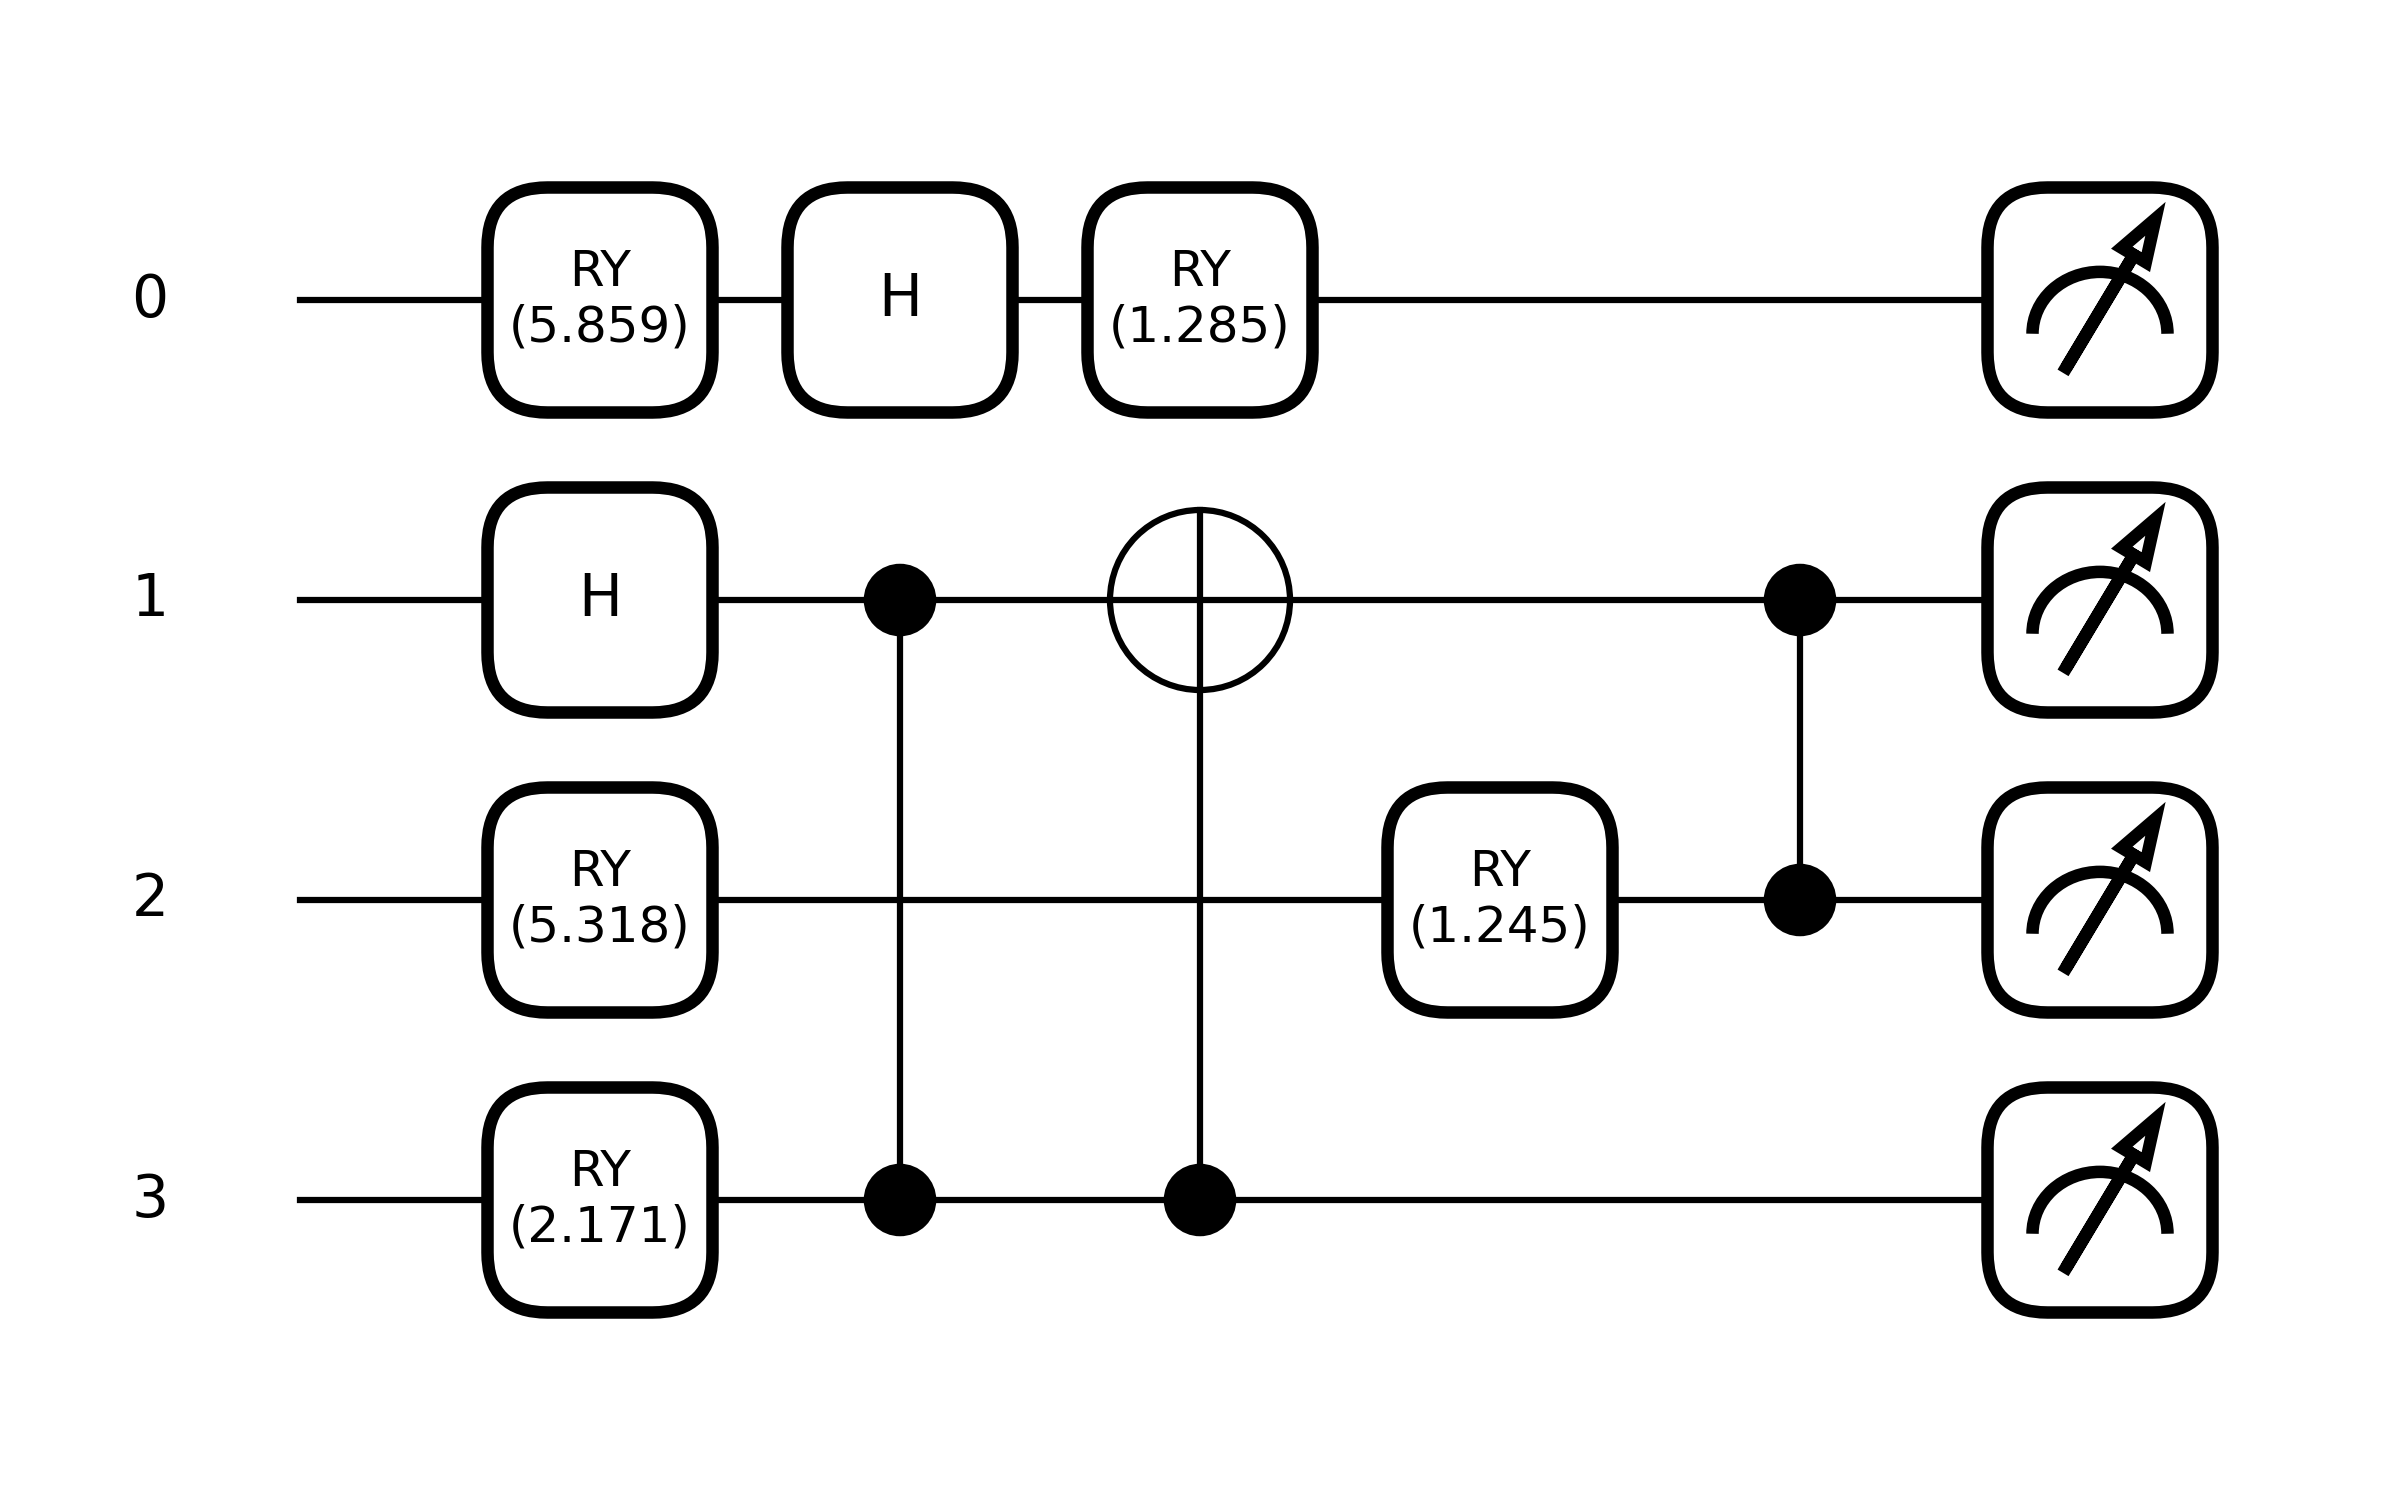
\includegraphics[width=\textwidth]{images/4-qubits-fidelity_target.png} %
    \caption{The target circuit of the 4-qubit state preparation} 
    \end{subfigure}
    \hspace{0.5cm}
    \begin{subfigure}[b]{0.475\textwidth}
    \centering
    \includegraphics[width=0.75\textwidth, height=0.6\textwidth]{images/8-qubits-fidelity_target.png}
    \caption{The target circuit of the 8-qubit state preparation} 
    \end{subfigure}
    \caption{The circuits used to generate the target states.}
    \label{fidelity_target}  
\end{center}
\end{figure}
\paragraph{Quantum State Preparation.} In quantum information theory, fidelity \citep{liang2019quantum} is an important metric to measure the similarity of two quantum states. By introducing fidelity as the performance index, we aim to maximize the similarity of the final state density operator with a certain desired target state. We first obtain the target state by randomly generating a corresponding circuit, and then with a limited number of sample circuits, we use the search methods to search candidate circuits that can achieve a fidelity higher than a certain threshold. During the search process, the fidelity can be directly used as a normalized reward function since its range is [0, 1]. Figure \ref{fidelity_target} shows the circuits used to generate the corresponding target states.

\paragraph{Max-cut Problems.} The max-cut problem \citep{poljak1995solving} consists of finding a decomposition of a weighted undirected graph into two parts (not necessarily equal size) such that the sum of the weights on the edges between the parts is maximum. Over these years, the max-cut problem can be efficiently solved with quantum algorithms such as QAOA \citep{villalba2021improvement} and VQE (using eigenvalues). In our work, we address the problem by deriving the Hamiltonian of the graph and using VQE to solve it. We use a simple graph with the ground state energy $-10 \ Ha$ for the 4-qubit experiment and a relatively complex graph with the ground state energy $-52 \ Ha$ in the case of the 8-qubit experiment. Furthermore, we convert the energy into a normalized reward function integral to the search process. The visual representations of these graphs are presented below:
\begin{figure}[ht]
\begin{center}
    \begin{subfigure}[b]{0.4\textwidth}
    \centering
    \includegraphics[width=\textwidth]{images/4-qubit-max_cut.png} %
    \caption{The 4-qubit max-cut graph} 
    \end{subfigure}
    \hspace{1cm}
    \begin{subfigure}[b]{0.4\textwidth}
    \centering
    \includegraphics[width=\textwidth]{images/8-qubit-max_cut.png}
    \caption{The 8-qubit max-cut graph} 
    \end{subfigure}
    \caption{The graphs of the experiments on max-cut problems.}
    \label{maxcut_graph}  
\end{center}
\end{figure}

\paragraph{Quantum Chemistry.} In the field of QC, VQE \citep{peruzzo2014variational, tilly2022variational} is a hybrid quantum algorithm for quantum chemistry, quantum simulations, and optimization problems. It is used to compute the ground state energy of a Hamiltonian based on the variational principle. For the 4- and 12-qubit quantum chemistry experiment, we use the Hamiltonian of the molecule $H_2$ and $LiH$ and its common approximate ground state energy $-1.136 \ Ha$ and $-7.88 \ Ha$ as the optimal energy. As for the 8-qubit experiment, we consider $n=8$ transverse field Ising model (TFIM) with the Hamiltonian as follows:
\begin{align}
    \mH = 
    \sum_{i=0}^7\sigma_z^i\sigma_z^{(i+1) \ mod \ 6} + \sigma_x^i\text{.}
\end{align}
We design some circuits to evaluate the ground state energy of the above Hamiltonian and get an approximate value $-10 \ Ha$ as the optimal energy. According to the approximate ground state energy, we can use our methods to search candidate circuits that can achieve the energy reaching a specific threshold. In the process of searching for candidates, the energy is normalized as a reward function with the range [0, 1] to guarantee search stability.

\subsection{Hyperparameters of Pre-training}
\label{pretraining_parameters}
Table \ref{table:appendix Description of hp} shows the hyperparameter settings of the pre-training model for 4-qubit and 8-qubit experiments.
\begin{table}[ht]
\centering
     \caption{Description of hyperparameters adopted for pre-training.}
    \begin{tabular}{p{0.2\textwidth}p{0.4\textwidth}p{0.2\textwidth}}
    \hline
     Hyperparameter & Hyperparameter explanation & Value for 4/8/12-qubit experiments\\
    \hline
    bs & batch size & 32\\
    epochs & traning epochs & 16\\
    dropout & decoder implicit regularization & 0.1\\
    normalize & input normalization & True\\
    input-dim & input dimension & 2+$\#$gates+$\#$qubits\\
    hidden-dim & dimension of hidden layer & 128\\
    dim & dimension of latent space & 16\\
    hops & the number of GIN layers ($L$ in eq.\ref{mlp}) & 5 \\
    mlps & the number of MLP layers & 2 \\
    \bottomrule
  \end{tabular}
\label{table:appendix Description of hp}
\end{table}

\subsection{Best Candidate circuits}
\textbf{Observation (5):} In Appendix \ref{Best candidate circuits}, we present the best candidate circuits acquired by each of the three methods for every experiment. These circuits exhibit a higher likelihood of being discovered by REINFORCE and BO in contrast to Random Search. This observation underscores the superior search capabilities of REINFORCE and BO in navigating the large and diverse search space generated by our approach, which is based on a random generator derived from a fixed operation pool. Unlike conventional approaches that adhere to layer-wise circuit design baselines, our method excels in discovering circuits with fewer trainable parameters. This characteristic is of paramount importance when addressing real-world optimization challenges in QAS. In conclusion, our approach not only enhances the efficiency of candidate circuit discovery but also accommodates the distinct characteristics of various problem domains through a large and diverse search space.
\label{Best candidate circuits}
\begin{figure}[ht]
\begin{center}
    \begin{subfigure}[b]{0.275\textwidth}
    \centering
    \includegraphics[width=\textwidth]{images/best_candidate/4-qubits-fidelity_best_candidate_77132.png}

    \caption{4-qubit state preparation}
    \end{subfigure}
    \hfill
    \begin{subfigure}[b]{0.275\textwidth}
    \centering
    \includegraphics[width=\textwidth]{images/best_candidate/4-qubits-maxcut_best_candidate_14109.png}
    \caption{4-qubit max-cut}
    \end{subfigure}
    \hfill
    \begin{subfigure}[b]{0.275\textwidth}
    \centering
    \includegraphics[width=\textwidth]{images/best_candidate/4-qubits-vqe_best_candidate_94071.png}
    \caption{4-qubit quantum chemistry}
    \end{subfigure}

    \begin{subfigure}[b]{0.275\textwidth}
    \centering
    \includegraphics[width=\textwidth, height=0.75\textwidth]{images/best_candidate/8-qubits-fidelity_best_candidate_2930.png}
    \caption{8-qubit state preparation}
    \end{subfigure}
    \hfill
    \begin{subfigure}[b]{0.275\textwidth}
    \centering
    \includegraphics[width=\textwidth,  height=0.75\textwidth]{images/best_candidate/8-qubits-maxcut_best_candidate_84948.png}
    \caption{8-qubit max-cut}
    \end{subfigure}
    \hfill
    \begin{subfigure}[b]{0.275\textwidth}
    \centering
    \includegraphics[width=\textwidth, height=0.75\textwidth]{images/best_candidate/8-qubits-vqe_best_candidate_75883.png}
    \caption{8-qubit quantum chemistry}
    \end{subfigure}
\end{center}
\caption{Best candidates of the six experiments in 50 runs.}
\label{best_candidates}
\end{figure}


%\subsection{Latent dimension analysis}
%\label{ld_analysis}
%Table \ref{Latent dimension analysis 4qubit} demonstrates a supplementary experiment for the pre-training process of the 4-qubit quantum circuit space. It can be observed from the experimental results that when the dimension of the latent space is too low, the training effect is very poor. This is because the dimension of the latent space cannot fully capture the characteristics of gate and adjacency matrices. As the dimension of the latent space increases, the model can capture the properties of the two matrices, so the performance gradually becomes better. However, continuing to increase the dimension will cause the dimension of the latent space to be too high, which will increase the difficulty of training. Simultaneously, an excessively high-dimensional latent space will increase the computational complexity, which is not what we expect, so we choose 16 as the potential feature dimension of the 4-qubit quantum circuit space. The 8-qubit one also shows similar results, but because the quantum circuit space of 8-qubit is more complex, the final selected feature dimension is 32.
%\begin{table} [ht]
%    \centering
%    \caption{Model performance with different latent dimensions measured by reconstruction accuracy, validity, and uniqueness. The model is QAS$_{URL}$ with KL divergence and has the same training epoch 16.}
%    \begin{tabular}{ c c|c c c c c}
%    \hline
%    \multirow{2}{*}{Qubit}&
%    \multirow{2}{*}{Dimension}&
%    \multicolumn{5}{c}{Metric}\\
%    \cline{3-7}
%    & & Accuracy$_{ops}$ & Accuracy$_{adj}$  & Validity & Uniqueness & Loss$_{avg}$\\
%    \hline
%    4 & 8 & 35.87 & 99.44 & 57.22 & 100 & 0.1753\\
%    \hline
%    4 & 16 & 99.99 & 99.99 & 86.91 & 100 & 0.0345\\
%    \hline
%    4 & 24 & 99.94 & 99.92 & 76.52 & 100 & 0.0371 \\
%    \hline
%    4 & 32 & 93.92 & 99.99 & 70.02 & 100 & 0.0429 \\
%    \hline
%    \label{Latent dimension analysis 4qubit}
%    \end{tabular}
%\end{table}

\begin{comment}
    \subsection{Supplement Comparison Experiments of QAS Methods}
\label{supplement}
\begin{figure}[ht]
\begin{center}
    \begin{subfigure}[b]{0.325\textwidth}
    \includegraphics[width=0.49\textwidth]{images/4-qubits-fidelity_regret_fidelity_from_200_with_var_willing.png} %
    \includegraphics[width=0.49\textwidth]{images/8-qubits-fidelity_regret_fidelity_from_200_with_var_willing.png} %
    \caption{State preparation}
    \label{state_preparation_regret}
    \end{subfigure}
    \hspace{0.01cm}
    \begin{subfigure}[b]{0.325\textwidth}
    \includegraphics[width=0.49\textwidth]{images/4-qubits-maxcut_regret_energy_from_100_with_var_willing.png}
    \includegraphics[width=0.49\textwidth]{images/8-qubits-maxcut_regret_energy_from_100_with_var_willing.png}
    \caption{Max-cut}
    \label{max-cut_regret}
    \end{subfigure}
    \hspace{0.01cm}
    \begin{subfigure}[b]{0.325\textwidth}
    \includegraphics[width=0.49\textwidth]{images/4-qubits-vqe_regret_energy_from_100_with_var_willing.png}
    \includegraphics[width=0.49\textwidth]{images/8-qubits-vqe_regret_energy_from_100_with_var_willing.png}
    \caption{Quantum chemistry} 
    \label{quantum_chemistry_regret}
    \end{subfigure}
    \caption{Regret values of the 6 sets of experiments. In (a), (b), and (c), the left side is the 4-qubit experiments and the right side is the 8-qubit experiments. The plots show the mean regret values of 50 independent runs (with different random seeds) given 1000 search queries. The shaded areas in the plots demonstrate the standard deviation of the regret value.}
    \label{regret}
\end{center}
\end{figure}
Figure \ref{regret} presents regret values for each experiment, representing the difference between actual results and their optimal counterparts. The plots intuitively illustrate that, with the exception of the 4-qubit max-cut experiment, the REINFORCE and BO algorithms excel in the search for quantum architectures, more approaching optimal values. This advantage becomes particularly pronounced in 8-qubit complex applications. Furthermore, our results demonstrate that both methods consistently yield smaller average regret variances than Random Search when searching for circuit architectures that closely approximate optimal values, underscoring their stability and reliability.

Table \ref{comparison2} and \ref{comparison3} are additional experiments max-cut and quantum chemistry for Table \ref{comparison1}. The experimental results show the same conclusions.
\begin{table}[ht]
\caption{Compare the QAS performance of different QAS methods for the 4-qubit max-cut.} % title name of the table
\centering % centering table  
\begin{tabular}{c c c cccccc} % creating 10 columns
\hline\hline
\addlinespace[0.5ex]
 Method & $F_{thr}$ & $N_{lbl}$ & $N_{rest}$ & $N_{>0.95}$ & $N_{eval}$ & $N_{QAS}$ & $P_{opt}$ & $N_{QAS}/N_{eval}$
\\ [0.5ex]  
\hline
\addlinespace[0.5ex]
% Entering 1st row  
\multirow{2}{*}{GNN$_{URL}$} & 0.85 & 1000 & 31338 & 19186 & 2000 & 612 & $\approx 1.00$ & 0.3060 \\[0.5ex] 
&0.9 & 1000 & 9778 & 7234 & 2000 & 743 & $\approx 1.00$ & 0.3715 \\[0.5ex]  
% Entering 2nd row  
\multirow{2}{*}{GSQAS$_{URL}$} & 0.85 & 1000 & 32012 & 18809 & 2000 & 588 & $\approx 1.00$ & 0.2940 \\[0.5ex]  
& 0.9 & 1000 & 13935 & 9479 & 2000 & 685 & $\approx 1.00$ & 0.3425 \\[0.5ex]  
\hline
\addlinespace[0.5ex]
QAS$_{URL\&RL}$ & - & 0 & 100000 & \textbf{37709} & 1000 & 727 & $\approx \textbf{1.00}$ & \textbf{0.7270} \\[0.5ex]
% [1ex] adds vertical space  
\hline % inserts single-line  
\end{tabular}
\label{comparison2}
\end{table}

\begin{table}[ht]
\caption{Compare the QAS performance of different QAS methods for the 4-qubit quantum chemistry.} % title name of the table
\centering % centering table  
\begin{tabular}{c c c cccccc} % creating 10 columns
\hline\hline
\addlinespace[0.5ex]
 Method & $F_{thr}$ & $N_{lbl}$ & $N_{rest}$ & $N_{>0.95}$ & $N_{eval}$ & $N_{QAS}$ & $P_{opt}$ & $N_{QAS}/N_{eval}$
\\ [0.5ex]  
\hline
\addlinespace[0.5ex]
% Entering 1st row  
\multirow{2}{*}{GNN$_{URL}$} & 0.6 & 1000 & 28322 & 11277 & 2000 & 376 & $\approx 0.98$ & 0.1880 \\[0.5ex] 
&0.675 & 1000 & 12303 & 5944 & 2000 & 458 & $\approx 0.98$ & 0.2290 \\[0.5ex]  
% Entering 2nd row  
\multirow{2}{*}{GSQAS$_{URL}$} & 0.6 & 1000 & 27201 & 10820 & 2000 & 387 & $\approx 0.98$ & 0.1935 \\[0.5ex]  
& 0.675 & 1000 & 12608 & 5966 & 2000 & 452 & $\approx 0.98$ & 0.2260 \\[0.5ex]  
\hline
\addlinespace[0.5ex]
QAS$_{URL\&RL}$ & - & 0 & 100000 & \textbf{22514} & 1000 & 531 & $\approx \textbf{0.98}$ & \textbf{0.5310} \\[0.5ex]
% [1ex] adds vertical space  
\hline % inserts single-line  
\end{tabular}
\label{comparison3}
\end{table}
\end{comment}

\end{document}